%TODOs:
%	* check the consistent usage of the N_V, N_C, ...
%	* ask for computation of the higher diffusion constant D for HSCM  
%	* use \sum\limits_{k = 1}^{N} for sum or integral limits 
% 	* use : in front of eg. definitions



\documentclass[a4paper,12pt,leqno, draft]{article}
% \documentclass[a4paper,12pt,leqno]{article}


% ----------------------- USED PACKAGES -----------------------
\usepackage{inputenc,fontenc}
\usepackage[a4paper,margin=3cm]{geometry}
\usepackage[english]{babel}

\usepackage{graphicx}
\graphicspath{{figures/}}
\newcommand{\figurewidth}{4}

\usepackage{subcaption}
\usepackage{nameref, hyperref}
\usepackage{algpseudocode}
\usepackage{amsmath, amssymb, mathtools, amsthm, bbm}
\usepackage{csquotes}
\usepackage{mathabx}
\usepackage{enumerate}   
\usepackage{enumitem}
\usepackage{booktabs}   
\usepackage{subfiles}



% -------------------- STRUCTURES -----------------------------
\theoremstyle{plain}
\newtheorem{theorem}{Theorem}[section]
\newtheorem{lemma}[theorem]{Lemma}
\newtheorem{proposition}[theorem]{Proposition}
\newtheorem{corollary}[theorem]{Corollary}
\newtheorem{model}[theorem]{Model}
\newtheorem{problem}[theorem]{Problem}
\newtheorem{algorithm}[theorem]{Algorithm}
\newtheorem{ode}[theorem]{ODE}

\theoremstyle{remark}
\newtheorem{remark}[theorem]{\bf Remark}
\newtheorem{definition}[theorem]{\bf Definition}

% ------------------ COMMANDS ---------------------------------

\newcommand{\R}{\mathbb{R}}
\newcommand{\N}{\mathbb{N}}
\newcommand{\Z}{\mathbb{Z}}
\newcommand{\Q}{\mathbb{Q}}
\newcommand{\dequ}{\mathrm{d}}
\newcommand{\F}{\mathbf{F}}
\DeclareMathOperator{\sgn}{sgn}
\DeclareMathOperator{\entspricht}{\: \wedge }
\DeclareMathOperator{\atanxy}{arctan2}
%\DeclareMathOperator{\norm[1]}{\lVert#1\rVert_{_{2}}}
\newcommand{\norm[1]}{\lVert#1\rVert_{_{2}}}
\newcommand{\infnorm[1]}{\lVert#1\rVert_{_{\infty}}}
%\newcommand{\qed}{\hfill \ensuremath{\Box}}
\setlength{\parindent}{0em} 



%% ----------------------------- START OF DOCUMENT ----------------------------------------- 

\begin{document}


\include{chapters/titlePage}
% \section*{Acknowledgements}

\tableofcontents 
%\newpage 
%\listoffigures 
%\newpage 
%\listoftables

%\section*{Nomenclature}

\begin{table}[h!]
\centering
\begin{tabular}{c p{12cm}} % l = left aligned, c = centered, r = right aligned
\hline
\textbf{abbreviation} & \multicolumn{1}{c}{\textbf{description}}\\ 
\midrule
PDE &  A partial differential equation is an equation that contains unknown multivariable functions and their partial derivatives. \\
SDE &  A stochastic differential equation is a differential equation in which one or more of the terms is a stochastic process, resulting in a solution that is also a stochastic process. \\
DF model & The discrete form model is a vertex cell model that is defined by a list of all wall points. \\
\bottomrule
\end{tabular}
\end{table}
%\section*{Mathematical conventions}

\begin{table}[h!]
\centering
\begin{tabular}{c p{12cm}} % l = left aligned, c = centered, r = right aligned
\hline
symbol & description \\ 
\midrule
$\vec{v}$ & Superscript arrows denote multidimensional variables \\[0.5em] 
$\dfrac{\partial f}{\partial v}$ & Partial derivative of a scalar function $f$ with respect to a one dimensional variable $v$ \\[0.5em] 
$\nabla_{\vec{v}} f$  & gradient $\nabla_{\vec{v}} f = (\frac{\partial f}{\partial v_1}, \ldots, \frac{\partial f}{\partial v_n})^T$, where $f$ is a scalar function and $\vec{v} = (v_1, \ldots, v_n)^T$  \\[0.5em]
$D_{\vec{v}} F$ & Jacobian matrix $D_{\vec{v}} F = \begin{pmatrix}
    \frac{\partial F_1}{\partial v_1} \cdots \frac{\partial F_1}{\partial v_n} \\
    \vdots \\
    \frac{\partial F_m}{\partial v_1} \cdots \frac{\partial F_m}{\partial v_n} \\
\end{pmatrix}$, where $\vec{v} = (v_1, \ldots, v_n)^T$ is a multidimensional variable and $F = (F_1, \ldots, F_m)^T$ is a vector valued function \\
$\Delta f$ & Laplacian of a scalar function $f$ \\ 
$2e-3$ & scientific notation for $2 \times 10^{-3} = 0.002$ \\
$\dequ \vec{B}_i(t)$ & two dimensional Brownian motion applied to cell $i$ at time $t$ in SDEs \\
$I_d$ & Identity matrix in $\R^{d \times d}$  \\
$\R_+$ & positive real numbers including $0$, i.e. $[0, \infty)$  \\
\bottomrule
\end{tabular}
\end{table}
% \section*{Overview - Bachelor's thesis }

\subsection*{Cell models}

Definitions of continuous \textbf{Centre Radius Form (CRF)}:

\begin{definition} \textbf{Centre radius form (CRF)} \label{def:CRF}  \\
	For a given point $\vec{c} \in \mathbb{R}^2$ and function $r: [0, 2\pi) \rightarrow (0, \infty)$ so that $r \in C^1([0, 2\pi))$, $r(0) = r(2\pi)$ and $r'(0) = r'(2\pi)$, the tuple $(\vec{c}, r)$ describes a cell in its centre radius form (CRF) with centre point $\vec{c}$ and radius $r(\phi)$ at angle $\phi \in [0, 2\pi)$ that is taken with the $x$ axis. \\
\end{definition}

and \textbf{Discrete Form (DF)}:

\begin{definition} \textbf{Discrete form (DF)} \label{def:DF}  \\
	An ordered sequence of points $C = (\vec{x}_1, \ldots , \vec{x}_N)$ is considered to be a cell in its discrete form (DF) if the polygon that results when connecting every point with its neighbours and $\vec{x}_1$ with $\vec{x}_N$ is simple and positively orientated. \\	
	Cells in the DF model are sometimes just called discrete cells. \\
\end{definition}

\begin{figure}[b!]
	\centering
	\hfill
	\begin{subfigure}{0.4\textwidth}
		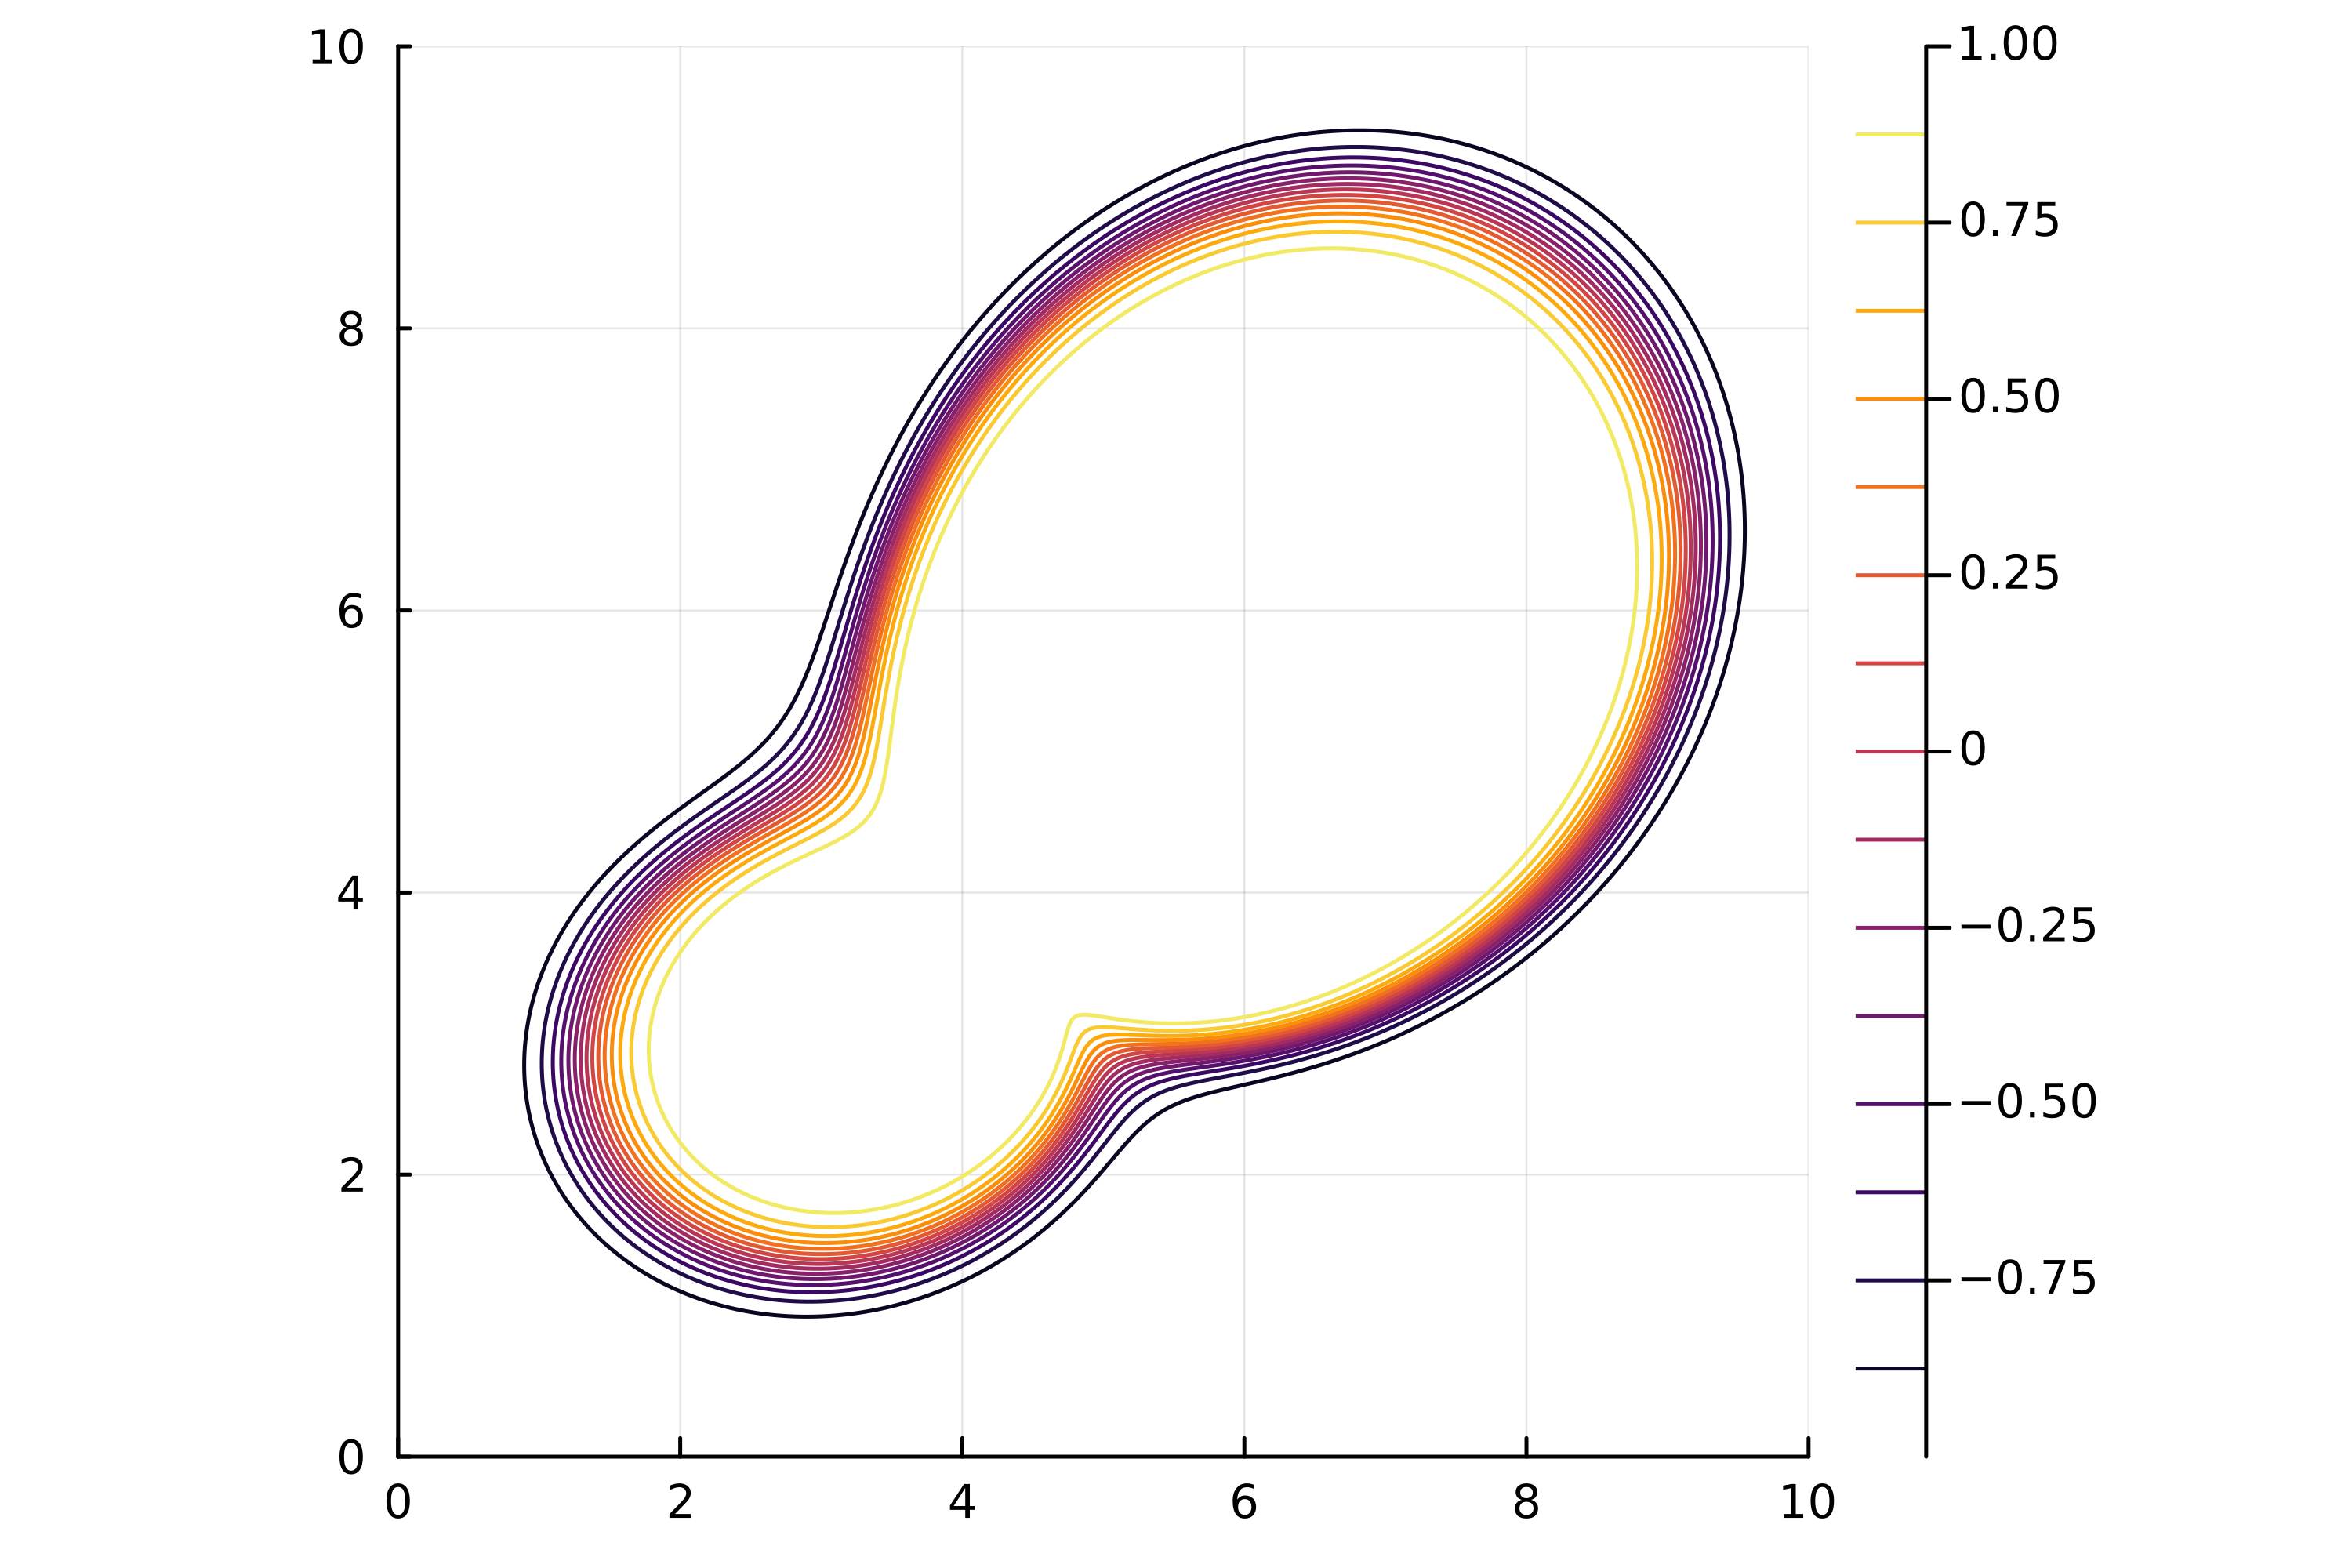
\includegraphics[width=\textwidth]{bachelors-thesis/model_illustrations/PhaseFieldModel.png}
		\caption{A contour plot of a phase field variable $\phi$ illustrates how cells can be modeled through phase field models. The cell's inside is the area where $\phi > 0$. The cell wall sits on the red line where $\phi = 0$. The outer lines display the smooth transition to the outside. }
	\end{subfigure}\hfill
	\begin{subfigure}{0.4\textwidth}
		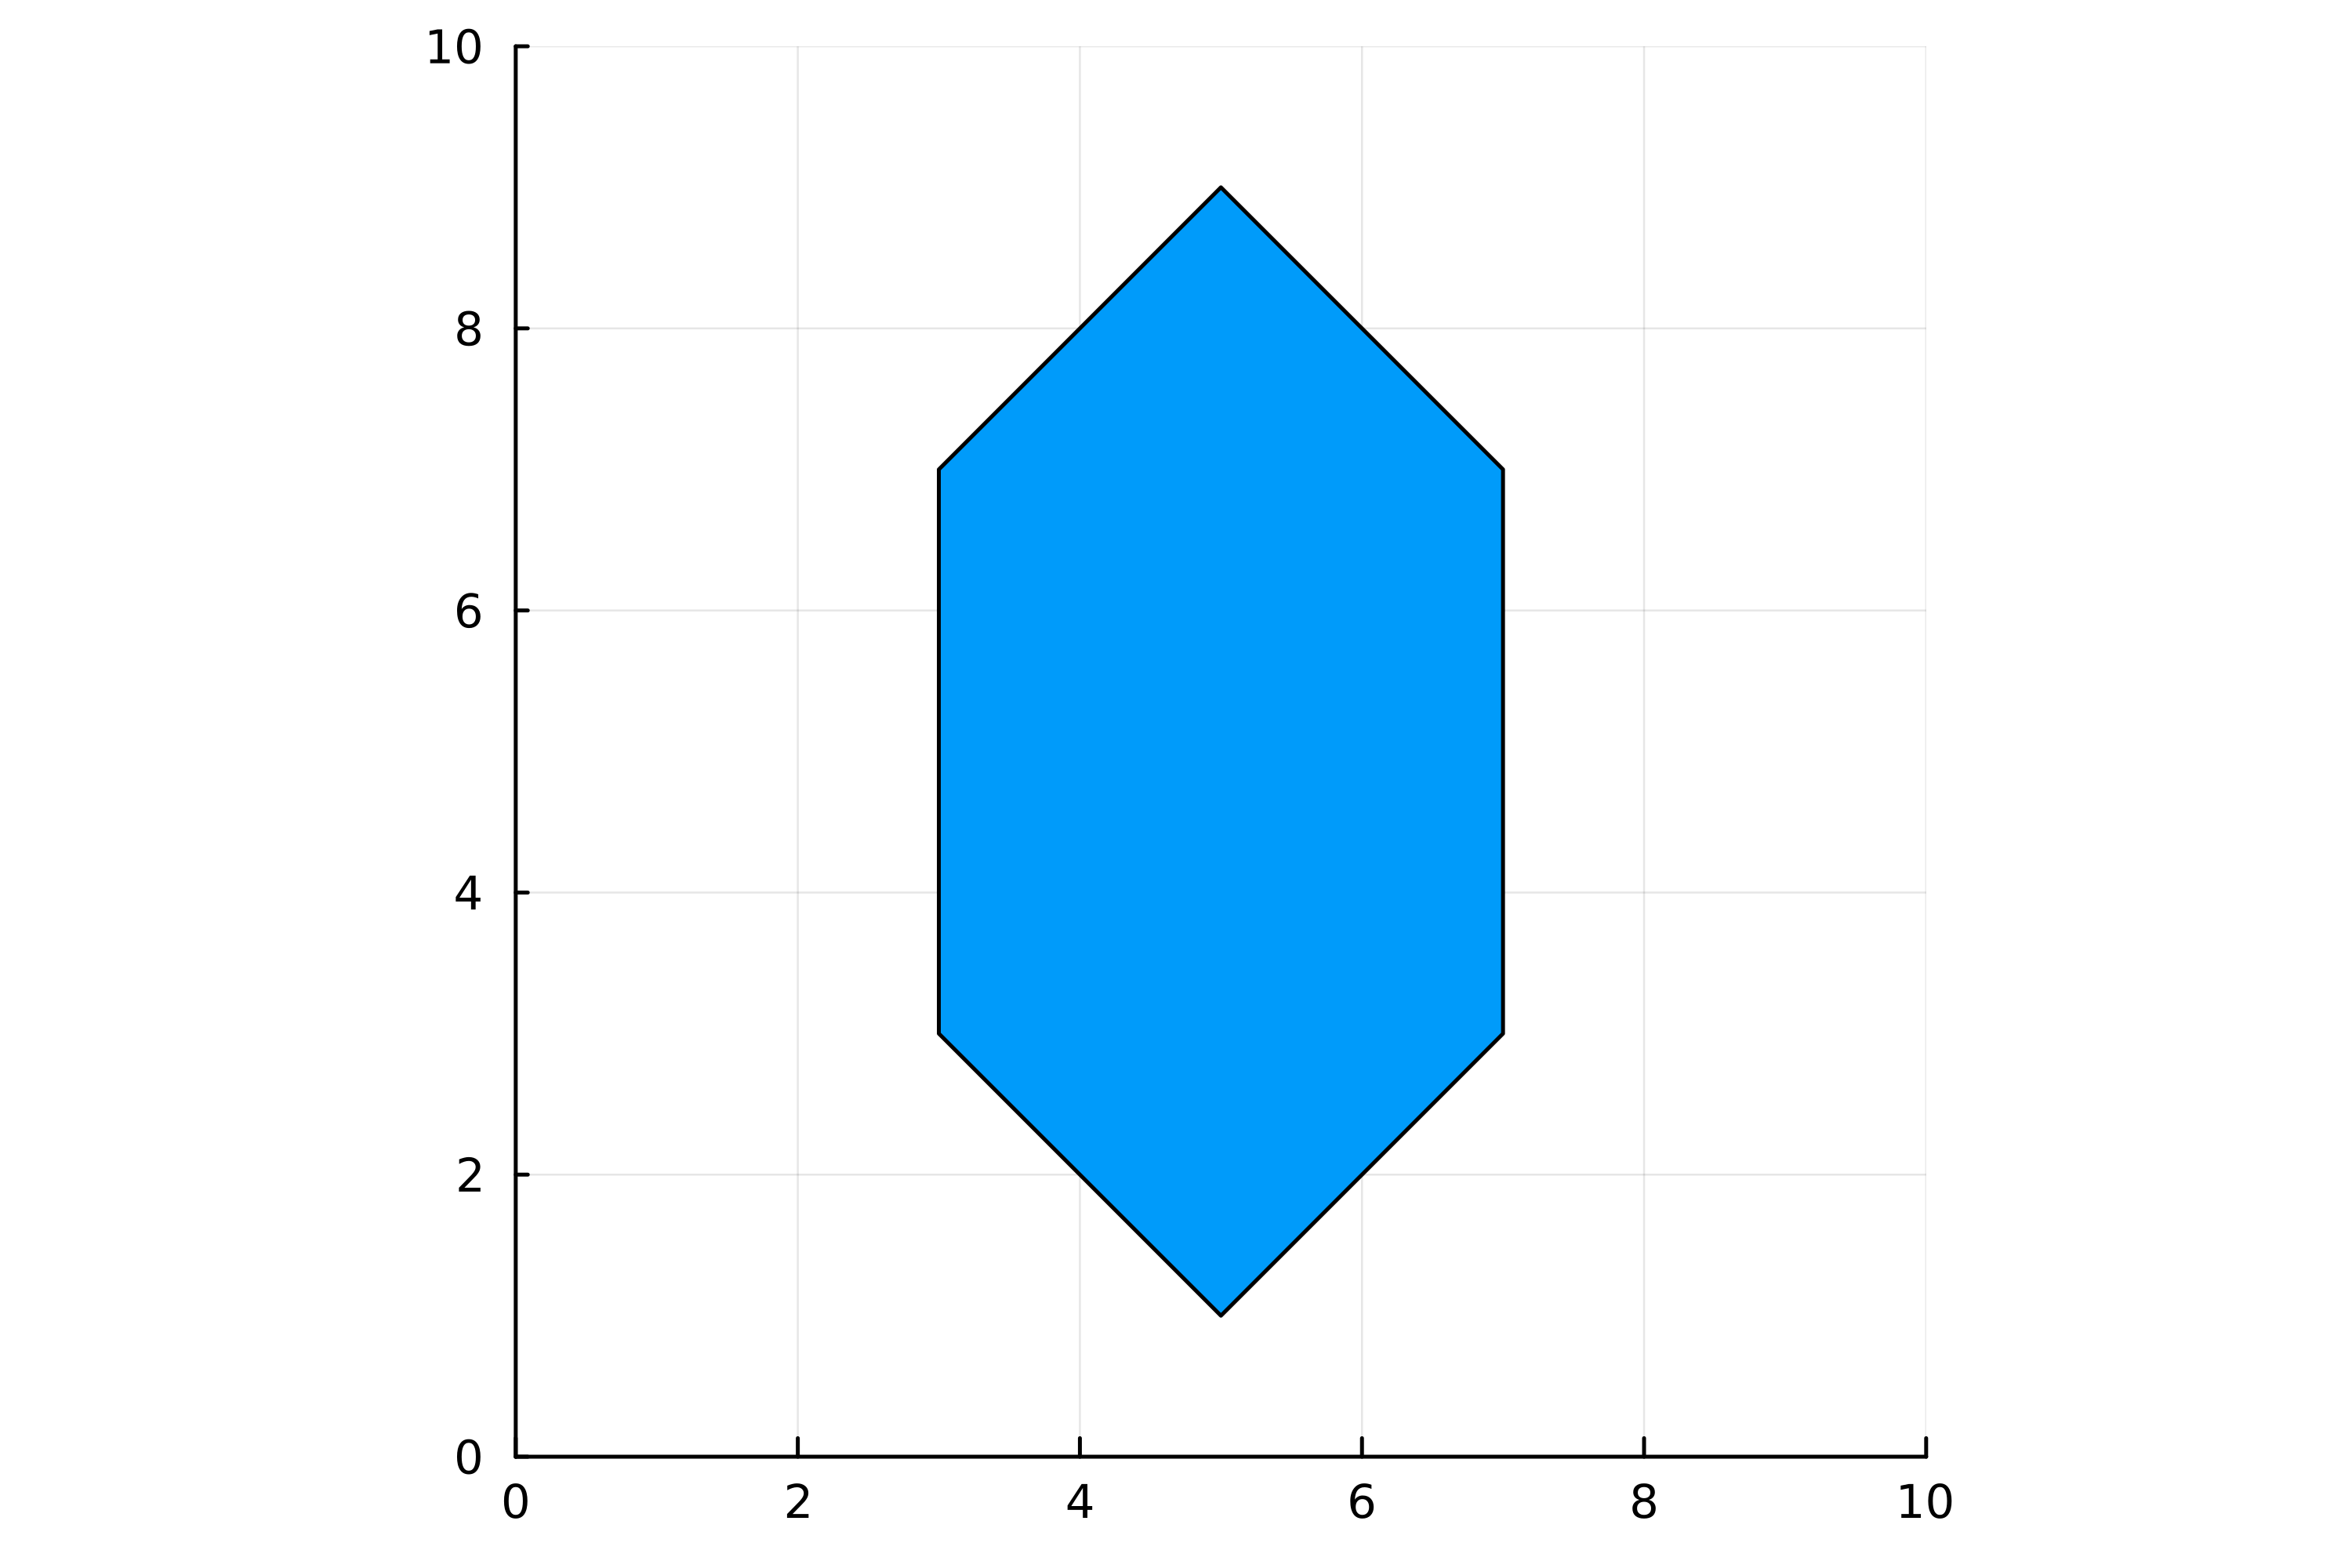
\includegraphics[width=\textwidth]{bachelors-thesis/model_illustrations/VertexModel.png}
		\caption{Another possibility to model cell forms are Vertex models. An example of this is shown here. This cell has six vertices. In order to model cell deformations, one can define forces that act on each vertex separately and thus cause them to move in an according direction. }
	\end{subfigure}
	\caption{To illustrate the models from the introduction, we can see a corresponding plot for each model. The sub figures (a) and (b) are concerned with the representation of cell shapes. In all sub figures, the axes denote the spatial $x$ and $y$ coordinates. } 
	\label{fig:model_illus}
\end{figure}

\newpage 
\subsection*{Derivation of forces}
First, we derived methods for area computation of both models. I will just focus on DF cells from now on. 
For DF cells, we can just apply the \textbf{shoelace lemma}: 
\begin{center}
    $A_C = \sum\limits_{i = 1}^{N} T_i = \frac{1}{2} \sum\limits_{i = 1}^{N} (y_i + y_{i+1})(x_i - x_{i+1}) = \frac{1}{2}\sum\limits_{i = 1}^{N} (x_i y_{i+1} - x_{i+1} y_i) $.
\end{center} 
\begin{figure}[h!]
    \begin{center}
        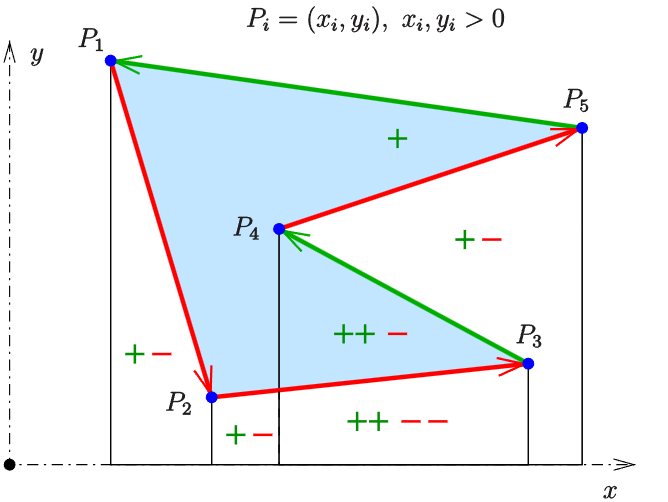
\includegraphics[width=8cm]{bachelors-thesis/shoelace.png}
        \caption{
            This figure shows a geometrical interpretation of the shoelace formula. In difference to the proposition, here the vertices are called $P_i$ and not $\vec{x}_i$. \\
            Source: \cite{ShoelaceFigure2022}}
        \label{fig:shoelace}
    \end{center}
\end{figure}

\newpage
Next, we derived a way to compute the \textbf{overlap} for DF cells: 
\begin{algorithm} \textbf{Computation of a discrete overlaps} \label{alge:discreteOverlap}
	\begin{itemize} 
		\itemsep0em 
		\item[] \text{INPUT:}
		\item Discrete cells  $C$and $\zeta$
		\item List $I$ of unused intersections of $C$ and $\zeta$ 
	\end{itemize}
	\begin{algorithmic}
		\Function{constructOverlap}{$C$, $\zeta$, $I$}		
			\State usedIntersections = List$\{$Intersection$\}$(I[1])
			\State newOverlap = List$\{$Vertices$\}$(I[1])
			\State currentIntersection = I[1]
			
			\For{counter = 1 : length(I)}
			
				\If{counter is even}
					\State newPath, newIntersection = findPath(currentIntersection, $C$, $I$)
				\Else
					\State newPath, newIntersection = findPath(currentIntersection, $\zeta$, $I$)
				\EndIf
				
				\State append!(newOverlap, newPath)
				\If{newIntersection == I[1]} 
					\State \Return newOverlap, usedIntersections
				\Else
					\State append!(newOverlap, newIntersection)
					\State append!(usedIntersections, newIntersection) 
					\State currentIntersection = newIntersection
				\EndIf
			\EndFor
		\EndFunction
	\end{algorithmic}
	\begin{itemize} 
		\itemsep0em 
		\item[] \text{OUTPUT:}
		\item A single intersection `newOverlap' which occurs between $C$ and $\zeta$ and which uses vertices from  $C$ and $\zeta$ as well as only intersections from $I$
		\item A list `usedIntersections' of all intersection that are used in `newOverlap'
	\end{itemize}	
\end{algorithm}

\begin{figure}[h!]
	\centering
	\begin{subfigure}{0.3\textwidth}
		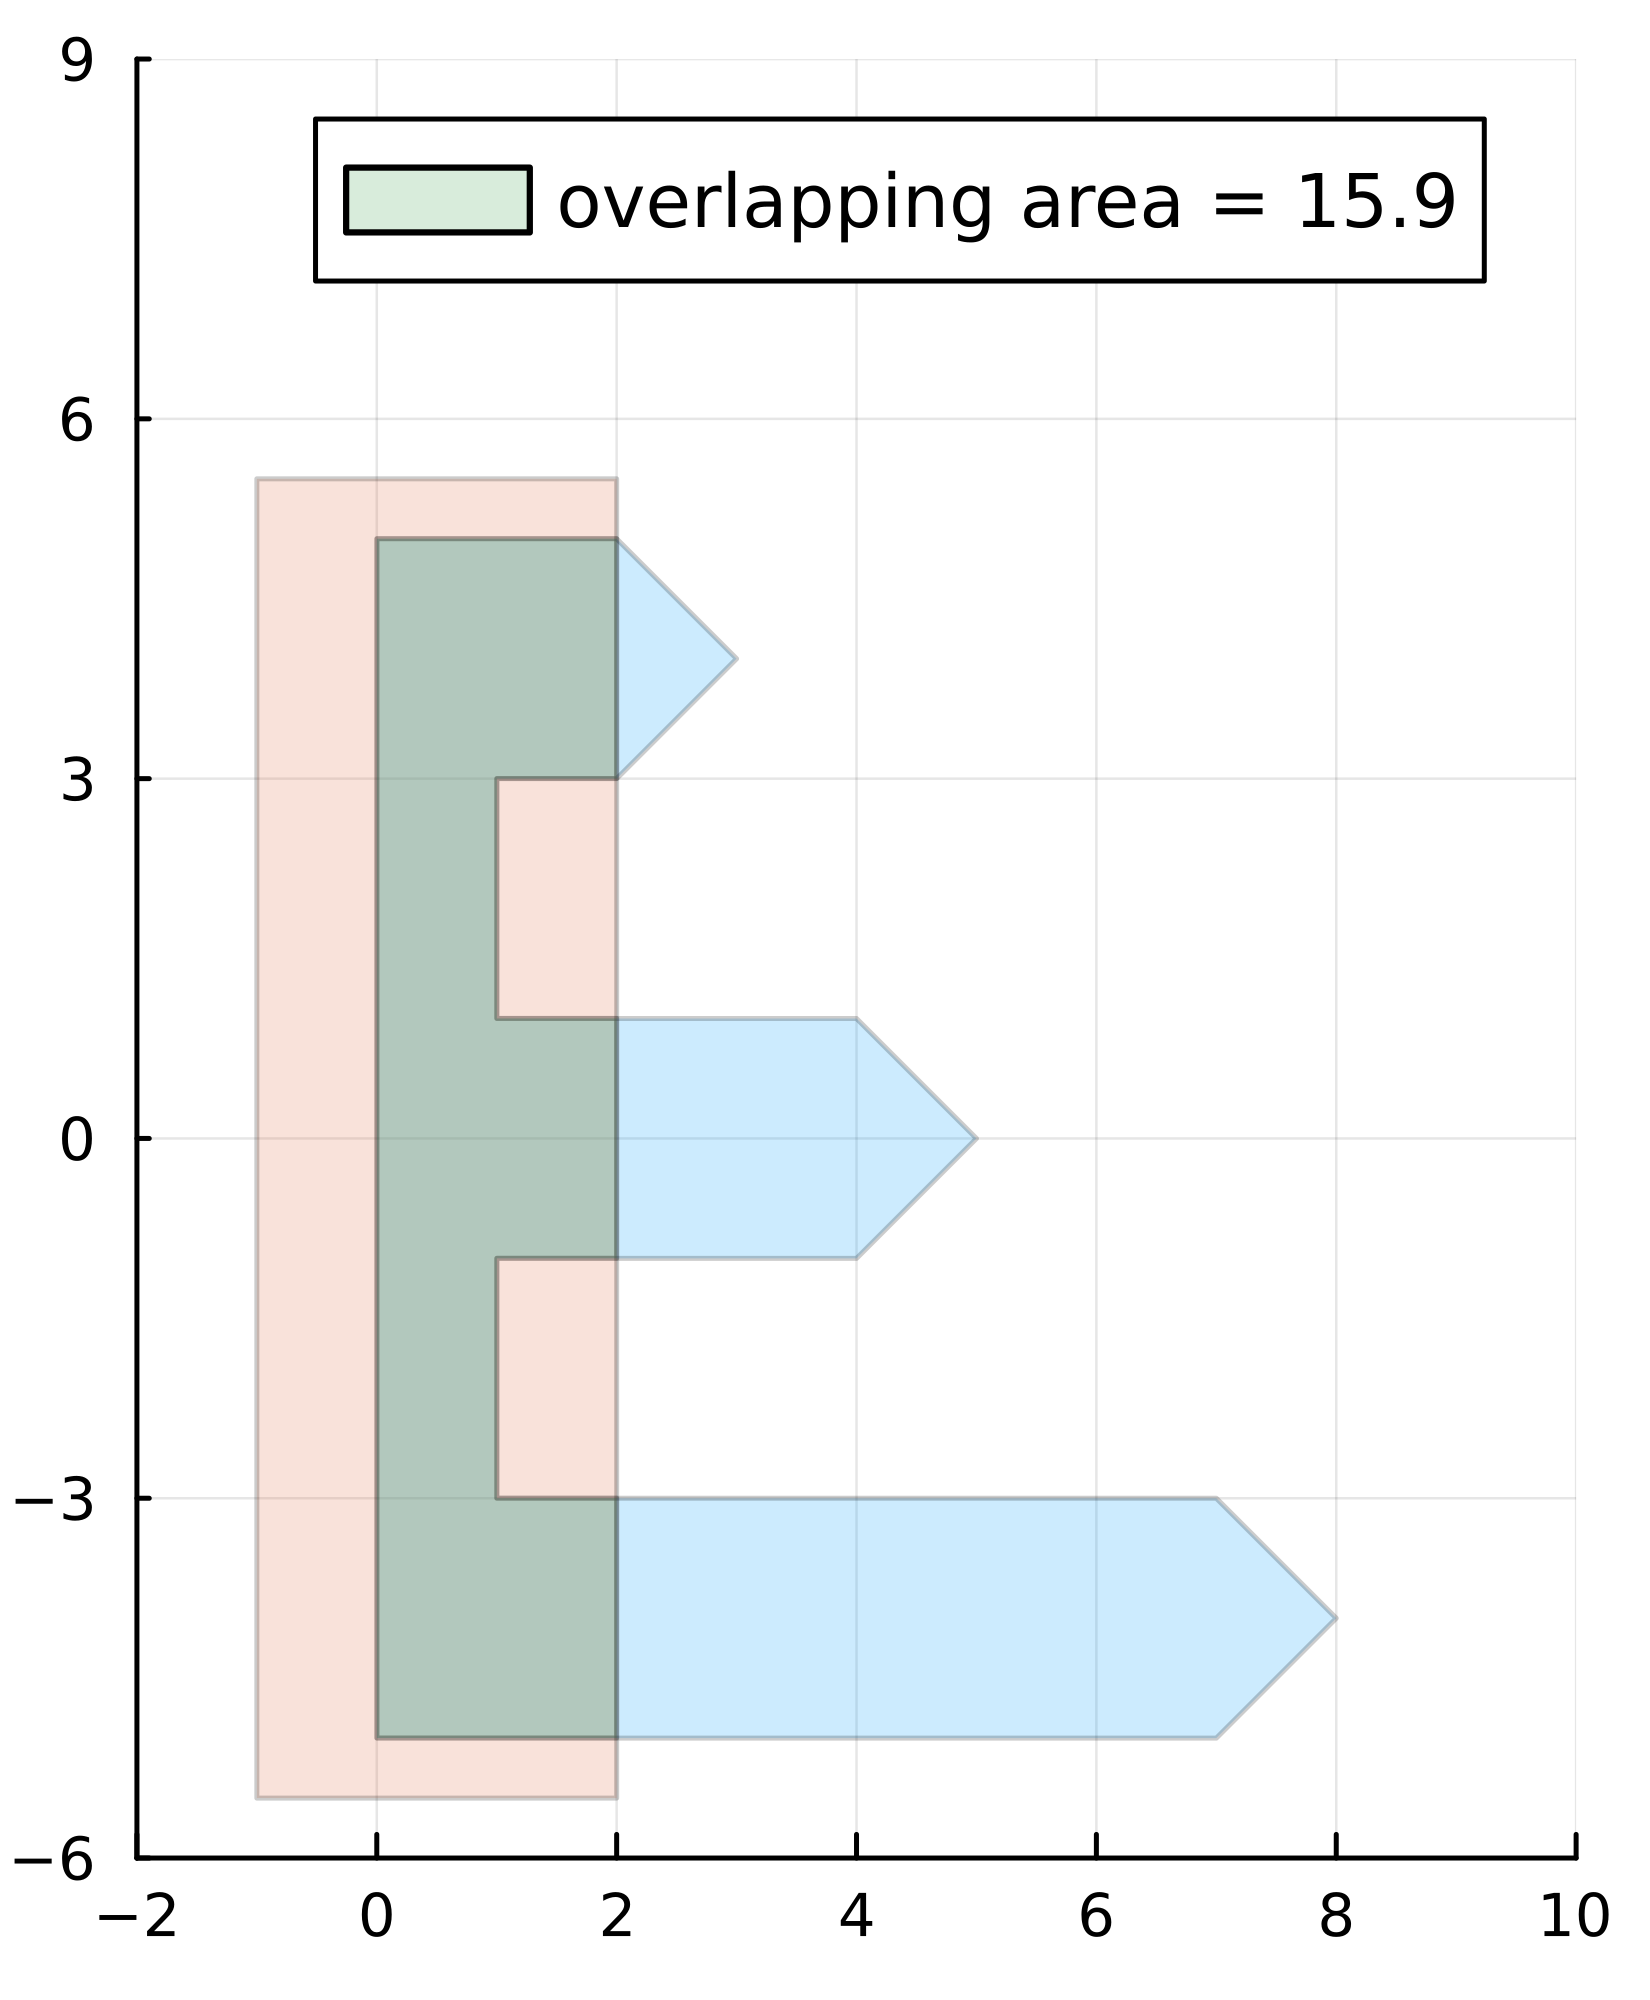
\includegraphics[width=\textwidth]{bachelors-thesis/discreteOverlap/discreteOverlapEx1.png}
	\end{subfigure}
	\hfill
	\begin{subfigure}{0.3\textwidth}
		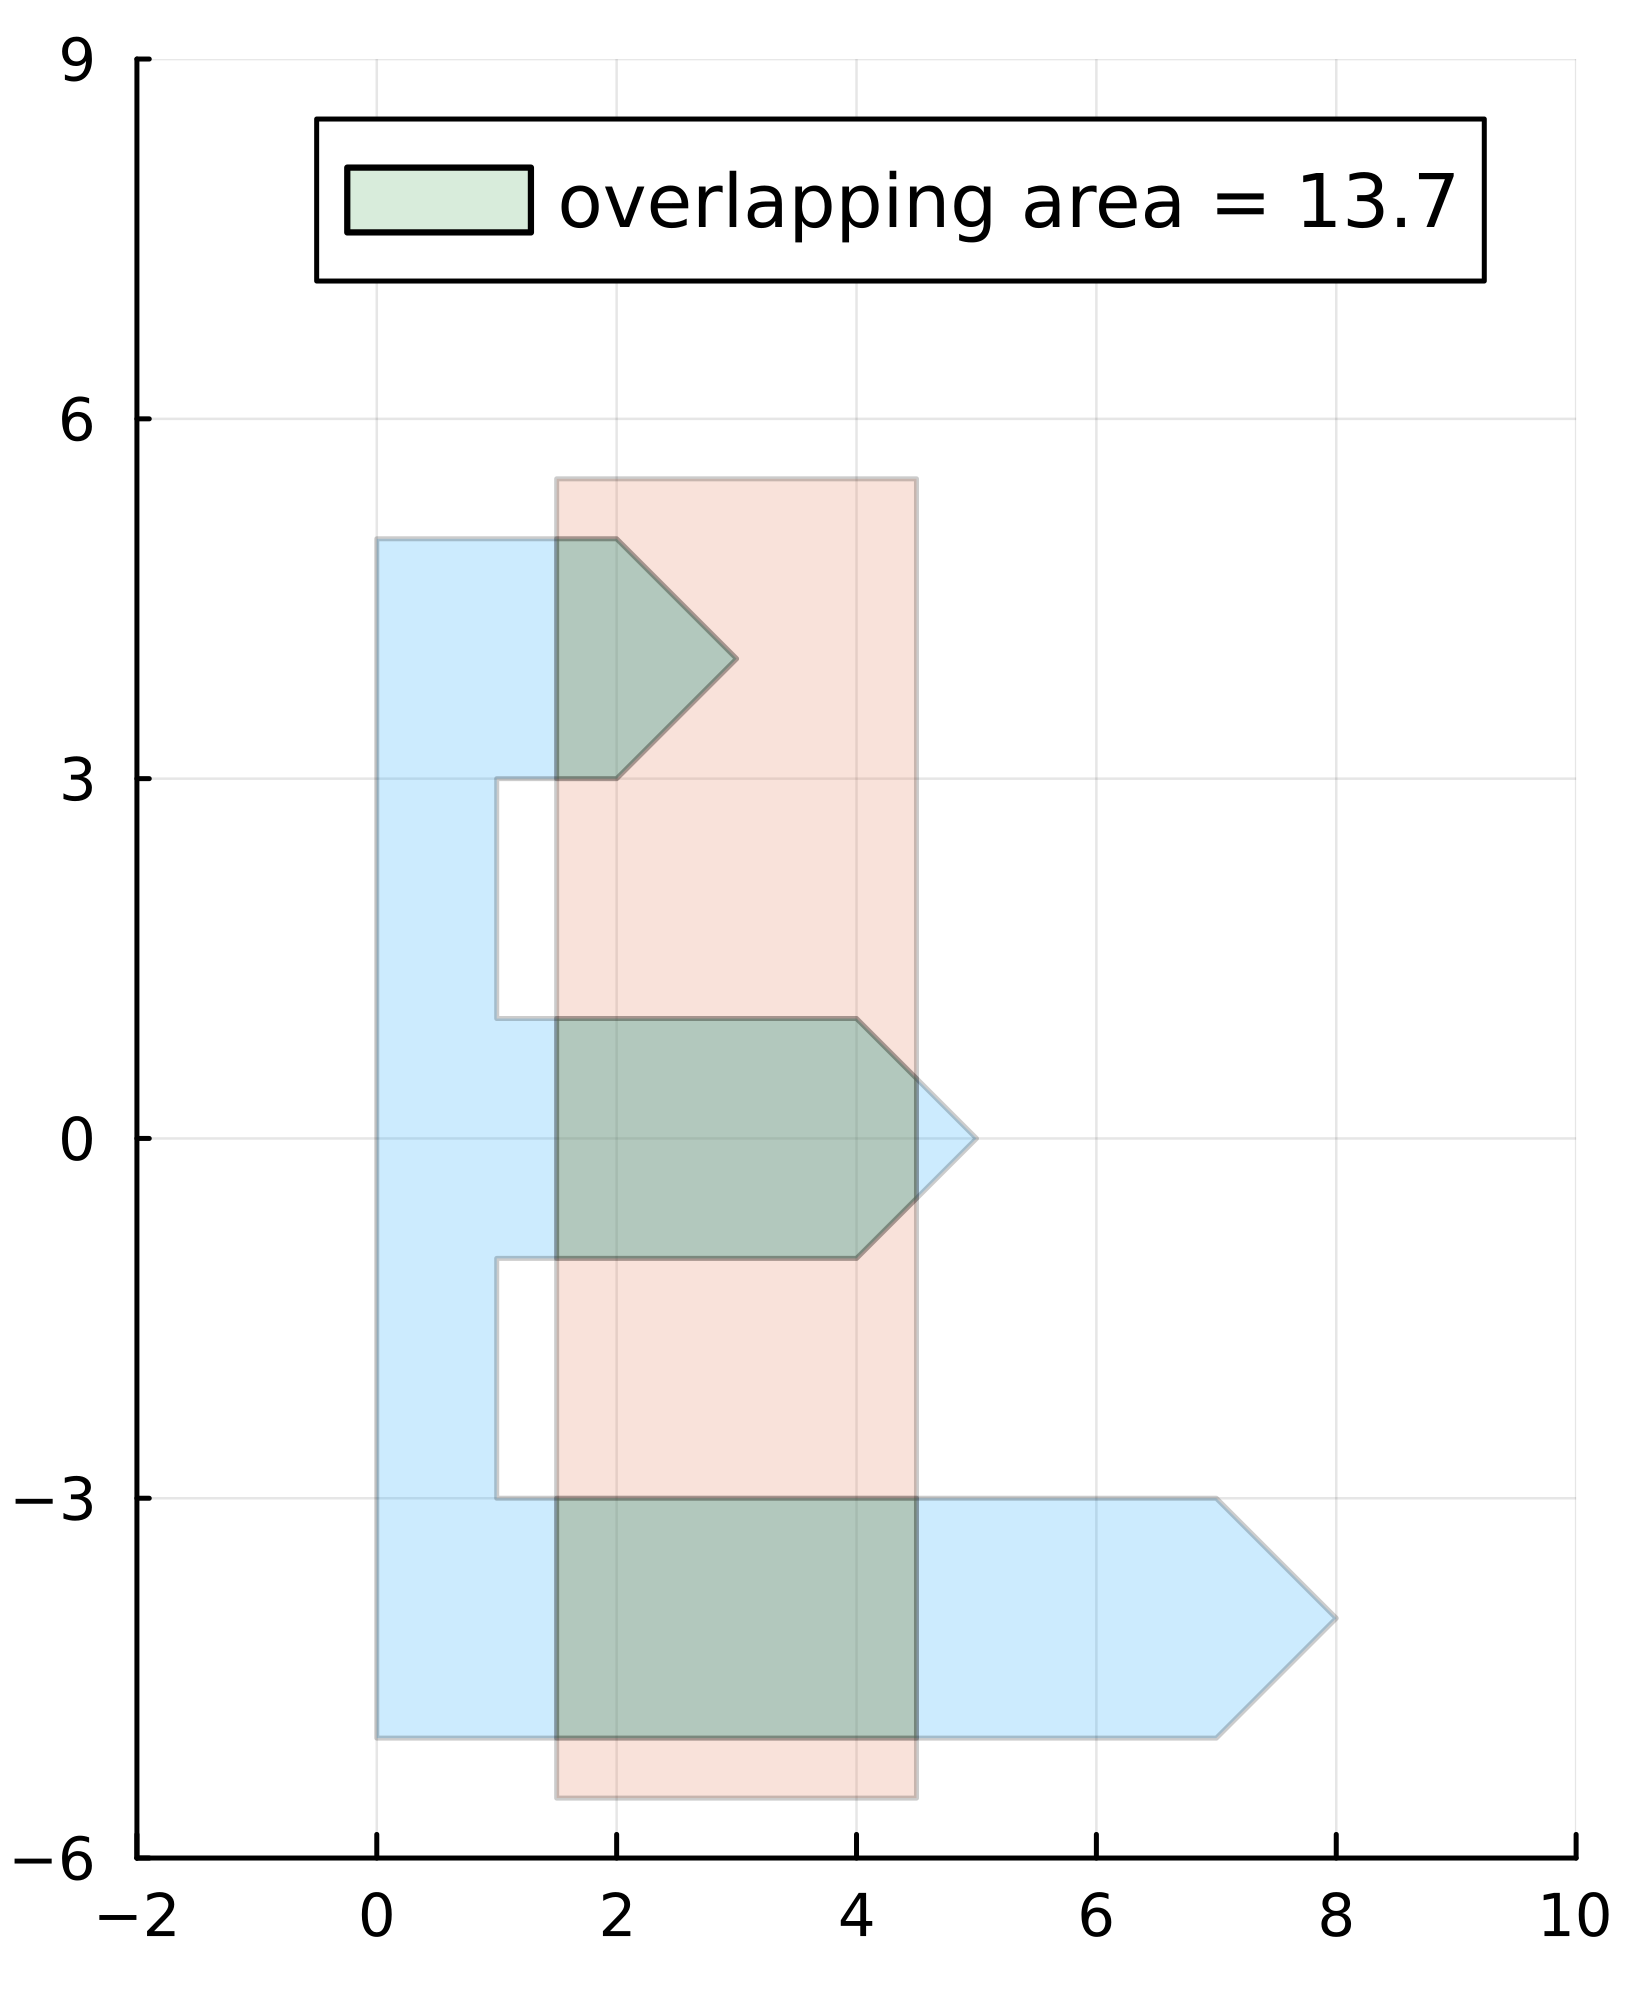
\includegraphics[width=\textwidth]{bachelors-thesis/discreteOverlap/discreteOverlapEx2.png}
	\end{subfigure}
	\hfill
	\begin{subfigure}{0.3\textwidth}
		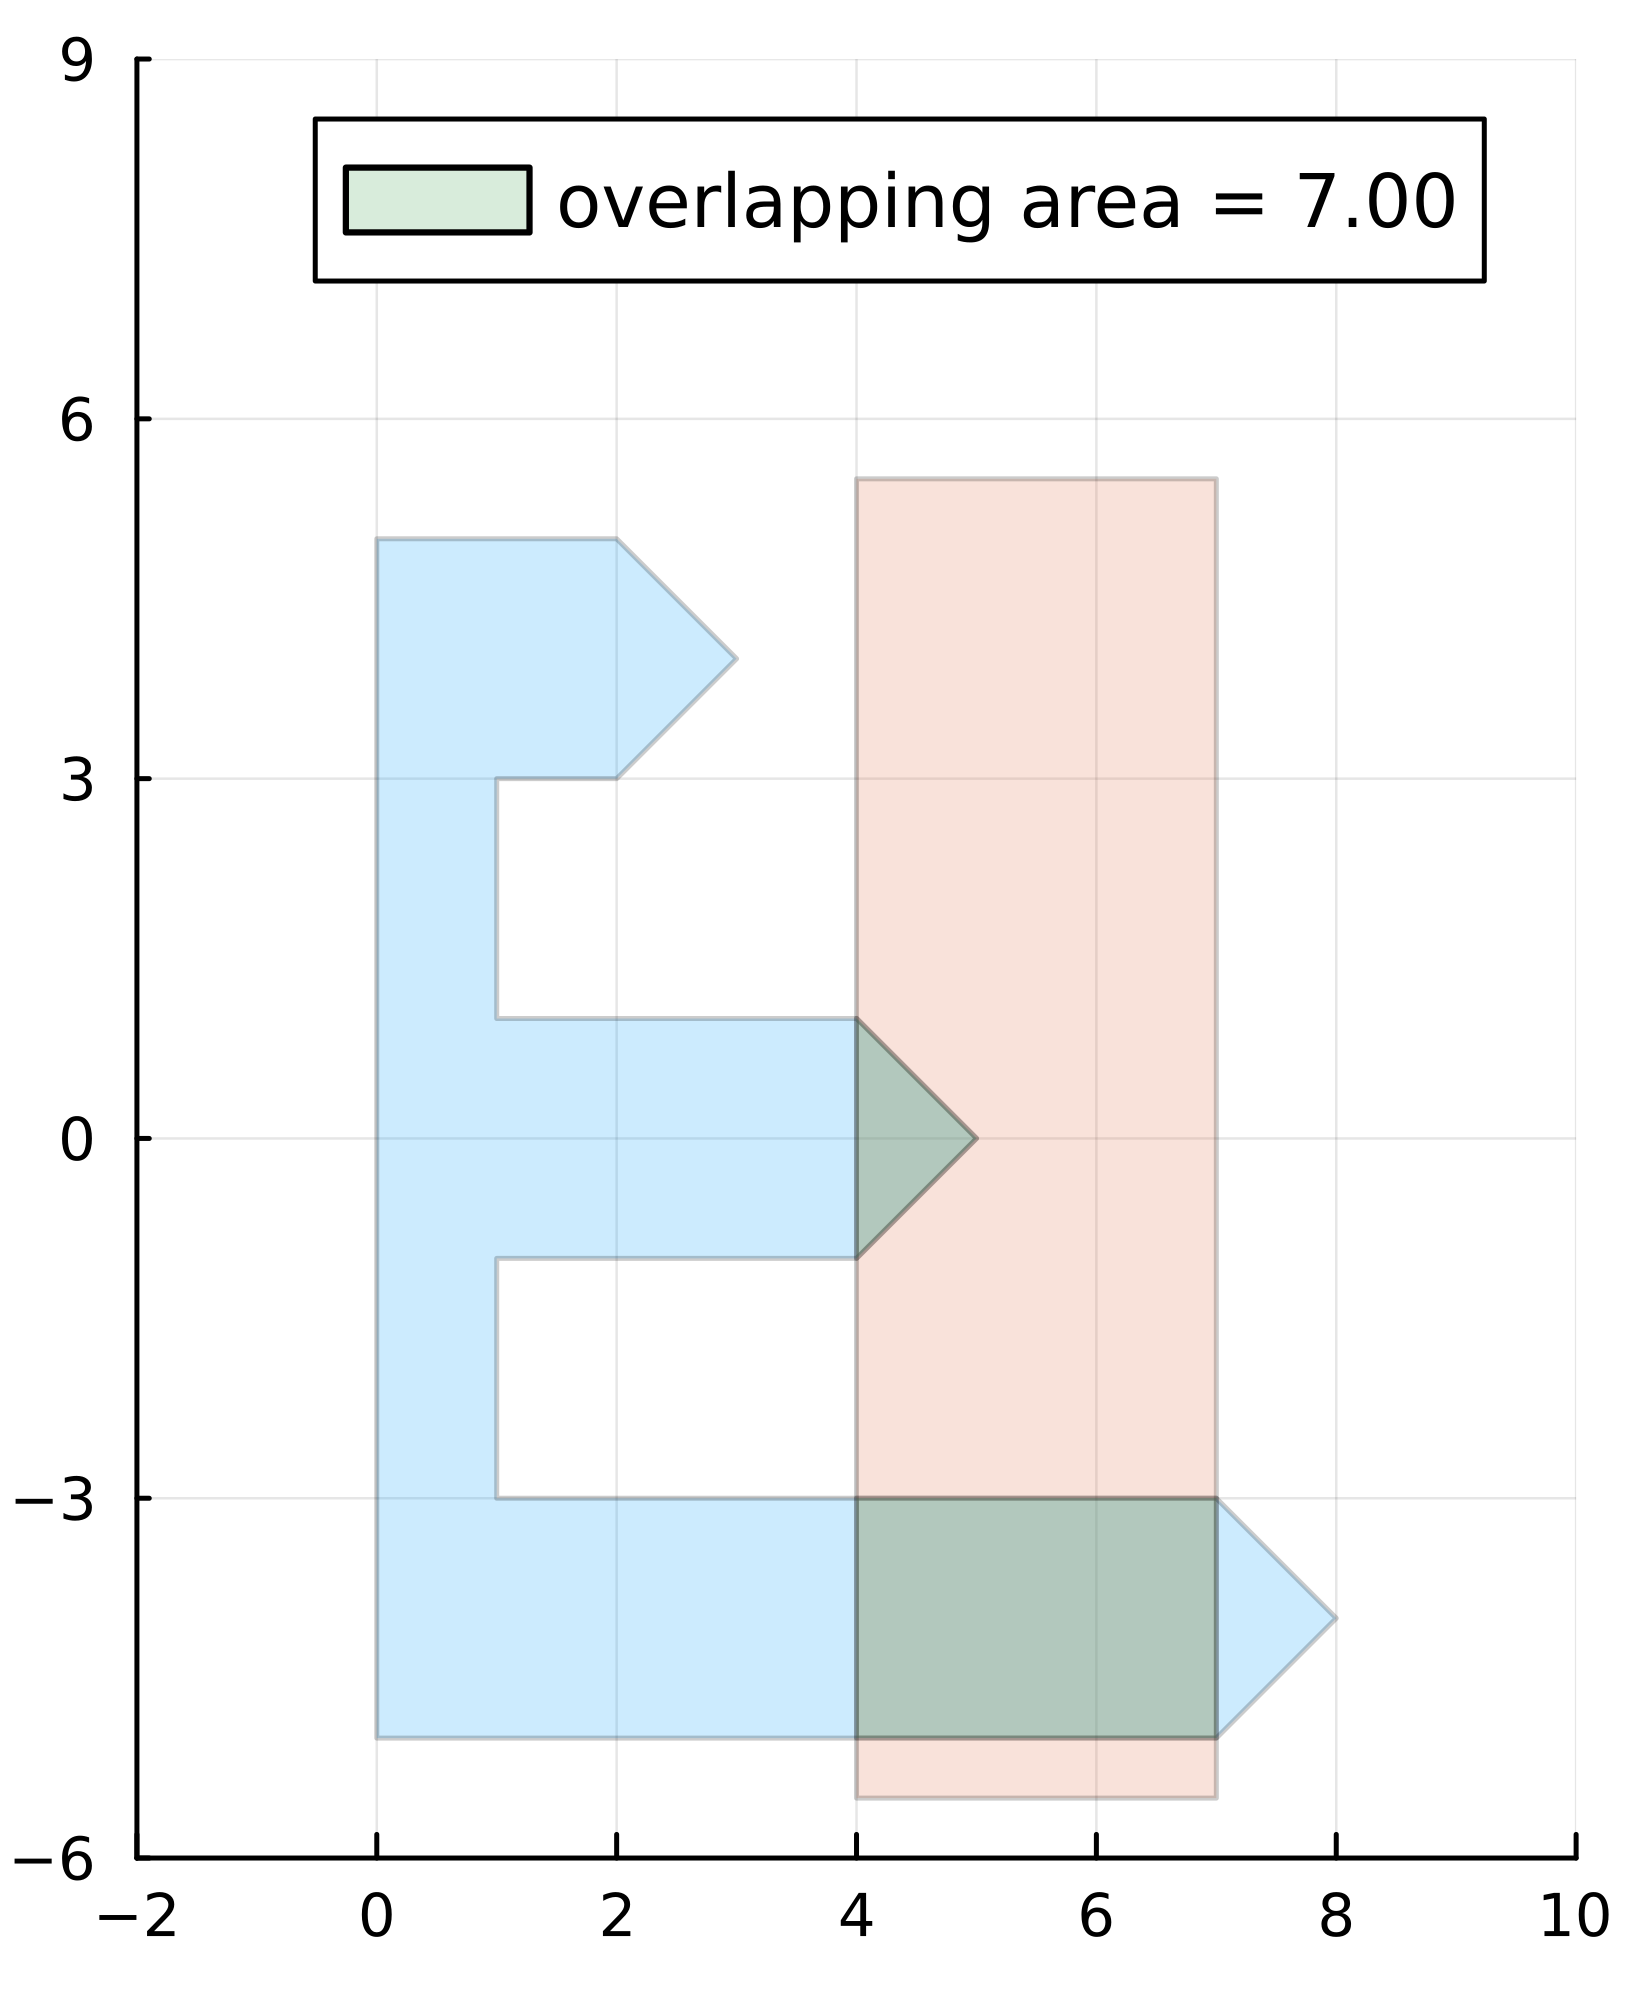
\includegraphics[width=\textwidth]{bachelors-thesis/discreteOverlap/discreteOverlapEx3.png}
	\end{subfigure}\hfill
	\caption{This figure shows 3 plots of 2 DF cells, shown in blue and red, each. One can see the calculated overlap in a green colour and the calculated area of the overlap is shown at the top of the plots. The red cell is shifted to the right in each subsequent plot, resulting in a change of the occurring overlap.}
	\label{fig:finalDiscreteOverlap}
\end{figure}

\newpage 
We defined how our \textbf{forces} look like using energies: 

\begin{definition} \textbf{Force function} \label{def:forceFunction}\\
	For a given energy $E_i$ of the $i$th cell, the force $F_{j}^{(E_i)}$ that describes the impact of $E_i$ on the $j$th vertex of the $i$th cell is given by
	\begin{center}
		$F_{j}^{(E_i)}(\vec{C}) := -\alpha_{E_i}(\vec{C}) \nabla_{\vec{x}_{ij}} E_i(\vec{C})$,
	\end{center}
	where $\alpha_{E_i} > 0$ denotes a positive scaling factor and $\nabla_{\vec{x}_{ij}}$ is the gradient for the $j$th vertex of cell $i$. 	\\
\end{definition}

and introduced the \textbf{area force} ...

\begin{proposition} \textbf{Area force} \\
	The gradient of $A_i$ with respect to the $j$th vertex of cell $i$ is given by 
	\begin{center}
		$\nabla_{\vec{x}_j} A_i(C_i) = \sgn(a(C_i) - a_i^{(d)}) \dfrac{1}{2} \begin{pmatrix} y_{i,j+1} - y_{i,j-1} \\ x_{i,j-1} - x_{i,j+1} \end{pmatrix}$. 
	\end{center}
	As a scaling factor, we choose
	\begin{center}
		$\alpha_{A_i}(C_i) := | a_i^{(d)} - a(C_i) |$. 
	\end{center}
	Thus, the area force reads 
	\begin{align}
		F_{j}^{(A_i)}(C_i) = \frac{1}{2}( a_i^{(d)} - a(C_i)) \begin{pmatrix} y_{i,j+1} - y_{i,j-1} \\ x_{i,j-1} - x_{i,j+1} \end{pmatrix}.
	\end{align}
	Proof.\\
	To reduce the notation effort, we neglect the subscript $i$, because we just consider a single cell.
	In order to compute $\nabla_{\vec{x}_j} | a^{(d)} - a(C) |$, let us first assume that $a^{(d)} \geq a(C)$. Then, one can calculate
	\begin{center}
		$
		\nabla_{\vec{x}_j} | a^{(d)} - a(C) | = - \nabla_{\vec{x}_j} a(C)
		= - \frac{1}{2}\sum\limits_{j = 1}^{N} \nabla_{\vec{x}_j} (x_{j} y_{j+1} - x_{j+1} y_{j})$ \\ \smallskip 
		$=- \frac{1}{2}\sum\limits_{j = 1}^{N} \begin{pmatrix} \partial_{x_j}  (x_{j} y_{j+1} - x_{j+1} y_{j})\\ \partial_{y_j} (x_{j} y_{j+1} - x_{j+1} y_{j})\end{pmatrix} 
		= - \dfrac{1}{2} \begin{pmatrix} y_{j+1} - y_{j-1} \\ x_{j-1} - x_{j+1} \end{pmatrix}
		$
	\end{center}
	
	Remember that $a^{(d)}$ is just an independent constant. In the other case, where $a^{(d)} < a(C(t))$, there is just a change in the sign. The combination of both cases yields the expression above. \\ 
	Since $- | a^{(d)} - a(C) | \sgn(a(C) - a^{(d)}) = a^{(d)} - a(C)$, we can conclude the area force. \\
	\qed
\end{proposition}

... the \textbf{edge force} \dots
\begin{proposition} \textbf{Edge force} \\
	The edge force is given by the formula
	\begin{align}
		F^{(E_{ij})}_j(C_i) = \dfrac{e_{j-1} - e_{i, j-1}^{(d)}}{e_{j-1}(C_i) } \begin{pmatrix} x_{j-1} - x_j \\ y_{j-1} - y_j\end{pmatrix} + 
		\dfrac{e_{j} - e_{i, j}^{(d)}}{e_{j}(C_i)} \begin{pmatrix} x_{j+1} - x_j \\ y_{j+1} - y_j\end{pmatrix}.
	\end{align}
	We choose $\alpha_{E_{ij}} := | e_{ij}^{(d)} - e_j(C_i) |$. \\
	Proof. \\
	Since this force acts on each cell individually, we can neglect the subscript $i$.
	The searched term has the following structure
	\begin{center}
		$F^{(E_{j})}_j(C) = - \alpha_{E_{j-1}} \nabla_{\vec{x}_j} E_{j-1}(C) - \alpha_{E_{j}} \nabla_{\vec{x}_j} E_{j}(C)$,
	\end{center}
	with the scaling factors $\alpha_{E_j}$ already defined in the proposition. \\	
	The partial derivatives of the edge length $e_j$ are
	\begin{center}
		$\partial_{x_j} e_j(C) = \partial_{x_j} ( (x_{j+1}- x_j)^2 + (y_{j+1} - y_j)^2)^{\frac{1}{2}} = \dfrac{ x_j - x_{j+1} }{ e_j(C) }$, \\
		$\partial_{y_j} e_j(C) = \dfrac{ y_j - y_{j+1} }{ e_j(C) }$. \\
	\end{center}
	This yields
	\begin{center}
		$ \nabla_{\vec{x}_j} E_{j} = sgn(e_{j}^{(d)} - e_j(C)) \nabla_{\vec{x}_j} - e_j(C)  = sgn(e_{j}^{(d)} - e_j(C))  \dfrac{1}{  e_j(C) } \begin{pmatrix} x_{j+1} - x_j \\ 	y_{j+1} - y_j \end{pmatrix}$,
	\end{center}
	and analogously
	\begin{center}
		$\nabla_{\vec{x}_j} E_{j-1} = sgn(e_{j-1}^{(d)} - e_{j-1}(C_i))  \dfrac{1}{  e_{j-1}(C) } \begin{pmatrix} x_{j-1} - x_j \\ 	y_{j-1} - y_j \end{pmatrix}$. 
	\end{center}
	This yields the edge force 
	\begin{center}
		$F_j^{(E_{j})}(C) = \dfrac{e_{j-1}(C) - e_{j-1}^{(d)}}{e_{j-1}(C)} 
		\begin{pmatrix}  x_{j-1} - x_j \\ y_{j-1} - y_j  \end{pmatrix} + 
		\dfrac{e_{j}(C) - e_{j}^{(d)}}{e_{j}(C)} 
		\begin{pmatrix}  x_{j+1} - x_j \\ y_{j+1} - y_j  \end{pmatrix}$.
	\end{center}
	\qed  
\end{proposition}

\dots the \textbf(interior angle force) \dots

\begin{proposition} \textbf{Interior angle force} \\
	The interior angle force is given by
	\begin{center}
		$F^{(I_{ij})}_j(C_i) = (\iota_{ij}^{(d)} - \iota_j(C_i))\left(
		\dfrac{1}{\norm[\vec{v}_1]^2} \begin{pmatrix}
			v_{1,y} \\-v_{1,x}
		\end{pmatrix}
		+ \dfrac{1}{\norm[\vec{v}_2]^2}\begin{pmatrix} -v_{2,y} \\ v_{2,x} \end{pmatrix}\right)
		$,
	\end{center}
	where $\vec{v}_1 = (v_{1,x}, v_{1,y})^T :=\vec{x}_{j-1} - \vec{x}_{j}$ and  $\vec{v}_2 = (v_{2,x}, v_{2,y})^T := \vec{x}_{j+1} - \vec{x}_{j}$. \\
	The scaling factor is defined as $\alpha_{I_{ij}} := | \iota_{ij}^{(d)} - \iota_j(C) |$. \\
	Proof. \\
	Again, we neglect the $i$, because we just consider one cell. 
	The goal is to determine the interior angle force
	\begin{center}
		$
		F^{(I_j)}_j(C) = - |\iota_{j}^{(d)} - \iota_j(C)| \nabla_{\vec{x}_j}I_j(C)
		$
	\end{center}
	Just like in the last forces, we use the $\sgn$ function to get rid of the absolute value, yielding
	\begin{center}
		$
		\nabla_{\vec{x}_j} I(C) = \sgn(\iota_j^{(d)}-\iota_j(C)) \nabla_{\vec{x}_j} (- \iota_j(C))
		$,
	\end{center}
	since the desired state is just a constant number. Since we have a minus in front of the gradient at the end of the equation, the searched force can be written as 
	\begin{center}
		$
		F^{(I_j)}_j(C) = (\iota_{j}^{(d)} - \iota_j(C)) \nabla_{\vec{x}_j}\iota_j(C)
		$.
	\end{center}
	The gradient of $\iota_j(C)$ is still missing. We will neglect the not differentiable modulo operator and must then compute
	\begin{center}
		$
		\nabla_{\vec{x}_j} (\atanxy(\vec{v}_1(C)) - \atanxy(\vec{v}_2(C))), 
		$
	\end{center}
	where $\vec{v}_1(C) = (x_{j-1} - x_{j} , y_{j-1} - y_{j})^T$ and $\vec{v}_2(C) = (x_{j+1} - x_{j} , y_{j+1} - y_{j})^T$. \\
	The function $\atanxy$ is partly defined and not truly differentiable. We still want to compute a gradient to use it for our interior angle force. Since $\atanxy(x,y) = \arctan(\frac{y}{x}) + \; constant$ almost everywhere, we will use the function $g(x,y) = \arctan(\frac{y}{x})$ for the derivation, because the different constants do not matter in the derivation. With $g$, we can rewrite $\iota_j(C) =g(x,y) \circ \vec{v}_1(C) - g(x,y) \circ \vec{v}_2(C) $. \\
	Thus, we need to determine 
	\begin{center}
		$
		\nabla_{\vec{x}_j} (g(x,y) \circ \vec{v}_1(C) - g(x,y) \circ \vec{v}_2(C)).
		$
	\end{center}
	The partial derivatives of $g$ are
	\begin{center}
		$\partial_{x} \arctan(\frac{y}{x}) = - \dfrac{y}{x^2} \dfrac{1}{1 + (\frac{y}{x})^2} = - \dfrac{y}{x^2 + y^2}$, \\
		$\partial_{y} \arctan(\frac{y}{x}) =  \dfrac{1}{x} \dfrac{1}{1 + (\frac{y}{x})^2} =  \dfrac{x}{x^2 + y^2}$.
	\end{center}
	It is easy to see that 
	\begin{center}
		$
		\partial_{x_j} \vec{v}_1(C) = \partial_{x_j} \vec{v}_2(C) = (-1,0)^T,
		\partial_{y_j} \vec{v}_1(C) = \partial_{y_j} \vec{v}_2(C) = (0, -1)^T. 
		$
	\end{center}
	This implies
	\begin{figure}[b!]
		\begin{center}
			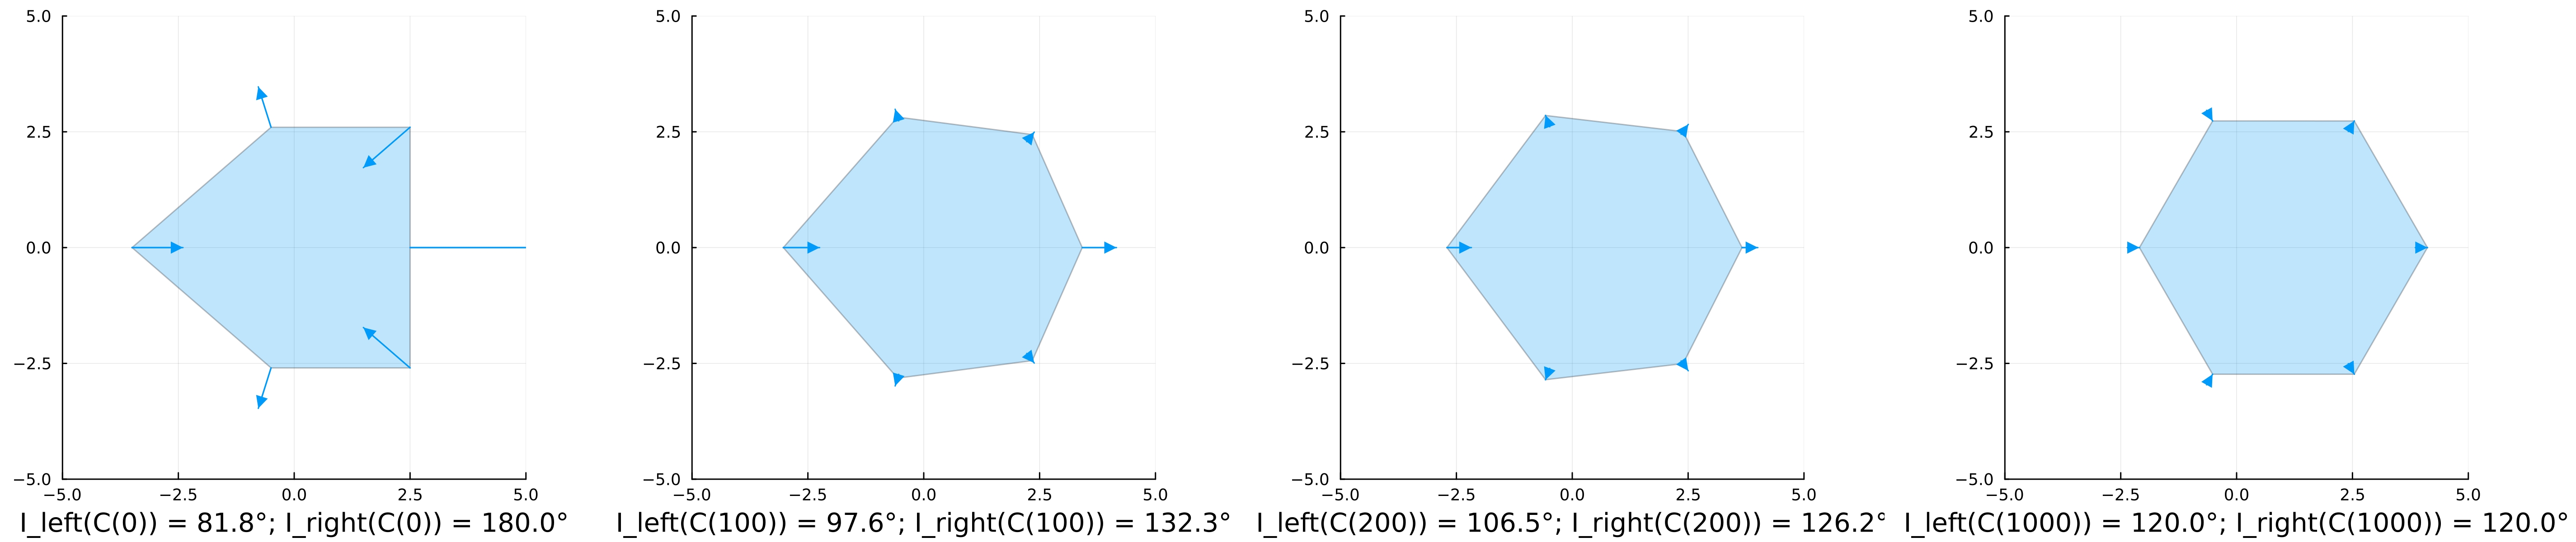
\includegraphics[width=15cm]{bachelors-thesis/forces/angle/angle1.png}
			\caption{This figure shows how the interior angle force acts on the vertices of a DF cell. The initial state can be seen in the first diagram. The desired state is the horizontally mirrored version of the initial state. Below each chart, we can see the current interior angles at $t \in \{0,50,100,3000\}$ of the two vertices that have the $y$ value zero. The desired states are $90$° for the right and $270$° for the left considered vertex. The interior angle force ensures that each interior angle transitions to the desired state over time, as we can see in this figure. }
			\label{fig:angleForce}
		\end{center}
	\end{figure}
	\begin{center}
		$
		\partial_{x_j} \iota_j(C) 
		\corresponds \partial_{x_j}( g\circ \vec{v}_1(C) - g \circ \vec{v}_2(C))$ \\ \smallbreak	
		$= (g'(\vec{v}_1(C)) \partial_{x_j} \vec{v}_1(C) - g'(\vec{v}_2(C))\partial_{x_j} \vec{v}_2(C) $ \\ \smallbreak	
		$= -(\partial_x g)(\vec{v}_1(C)) + (\partial_x g)(\vec{v}_2(C))$\\ \smallbreak 
		$= \dfrac{ v_{1,y} }{ v_{1,x}^2 + v_{1,y}^2 } - \dfrac{v_{2,y}}{v_{2,x}^2 + v_{2,y}^2}
		$,
	\end{center}
	using the multidimensional chain rule. In a similar fashion, we obtain
	\begin{center}
		$
		\partial_{y_j} \iota_j(C) = -\dfrac{v_{1,x}}{v_{1,x}^2 + v_{1,y}^2} + \dfrac{v_{2,x}}{v_{2,x}^2 + v_{2,y}^2}.
		$
	\end{center}
	Together this yields
	\begin{center}
		$
		\nabla_{\vec{x}_j} \iota_j(C) = \dfrac{1}{\norm[\vec{v}_1]^2} \begin{pmatrix} v_{1,y} \\ - v_{1,x} \end{pmatrix} + 
		\dfrac{1}{\norm[\vec{v}_2]^2} \begin{pmatrix} -v_{2,y} \\ v_{2,x} \end{pmatrix},
		$
	\end{center}
	which corresponds to the term from the proposition.\\
	\qed 
\end{proposition}

\dots and last but not least the \textbf{overlap force}

\begin{proposition} \textbf{Overlap force} \\
    The overlap force $F_j^{(O_i)}$ that acts on $\vec{x}_{ij}$ is given by
   \begin{align}
       F_j^{(O_i)}(\vec{C}) = \sum\limits_{m=1, m\neq i}^{M} ( \sum\limits_{D_k \in \Omega_{im}} - \mathbbm{1}_{\omega_{ik}}(\vec{x}_{ij})  a(D_k)\nabla_{\vec{d}_{l}} a(D_k)),
   \end{align}
   with $\nabla_{\vec{d}_{l}} a(D_k)$ given as
   \begin{center}
       $\nabla_{\vec{d}_{l}} a(D_k) = 
           \dfrac{1}{2}\begin{pmatrix}	d_{l+1}^{y} - d_{l-1}^{y} \\d_{l-1}^{x} - d_{l+1}^{x}	\end{pmatrix},
       $
   \end{center}
   with $\vec{d}_{l}$ being the corresponding vertex to $\vec{x}_{ij}$ in the according overlap and $\vec{d}_{l-1}$ and $\vec{d}_{l+1}$ being the vertices before and after $\vec{d}_{l}$. \\
   Proof. \\
   Instead of just using one scaling factor for each vertex, we will use a scaling factor $\alpha_{O_i, D_k} = a(D_k)$ for each individual overlap $D_k$. \\
   For all vertices $\vec{x}_{ij} \notin \omega_{ik}$, that are not included in the overlap $D_k$, the force is zero, because a change of position would not impact the area of the overlap in this case. This produces the indicator function $\mathbbm{1}_{\omega_{ik}}(\vec{x}_{ij})$ in the formula, that makes the force vanish for $\vec{x}_{ij} \notin \omega_{ik}$. \\
   Per definition of $\omega_{ik}$, we can always find an overlap vertex $\vec{d}_l$ that corresponds to $\vec{x}_{ij}$ if $\vec{x}_{ij} \in \omega_{ik}$. In this case, we can apply the gradient with respect to $\vec{d}_l$ on the area functional of $D_k$, to compute the direction of the fastest descent. \\	
   Thus, we must solve 
   \begin{center}
       $
       F_j^{(O_i)}(\vec{C}) = \sum\limits_{l=1, l\neq i}^{M} ( \sum\limits_{D_k \in \Omega_{il}} -\mathbbm{1}_{\omega_{ik}}(\vec{x}_{ij}) a(D_k) \nabla_{\vec{d}_l} a(D_k)).
       $
   \end{center}
   We can use the gradient computation shown in the area force, to determine
   \begin{center}
       $
       \nabla_{\vec{d}_l} a(D_k) = \frac{1}{2} 
       \begin{pmatrix}	d_{l+1}^{y} - d_{l-1}^{y} \\d_{l-1}^{x} - d_{l+1}^{x}	\end{pmatrix}
       $.
   \end{center}
   \qed
\end{proposition}

\newpage 
\subsection*{The interactive system} 
\begin{model} \textbf{First interacting system} \label{model:interaction1}\\ 
	The sum of all derived forces yields the first interacting system
	\begin{align}
		d\vec{x}_{ij}(t) =  F^{(A_i)}_j(C_i) + F^{(E_{ij})}_j(C_i) +F^{(I_{ij})}_j(C_i) +10 F^{(O_i)}_j(C_i) + \sqrt{2D} dB_t^{(i)}, \label{eq:interaction1}
	\end{align}
	where $\vec{x}_{ij}$ again stands for the vertex $j$ of the $i$th cell, $(1\leq i \leq9, \; 1\leq j \leq 20)$. 
\end{model}

and then made a rescaling which balanced all forces 
\begin{figure}[h!]
	\begin{center}
		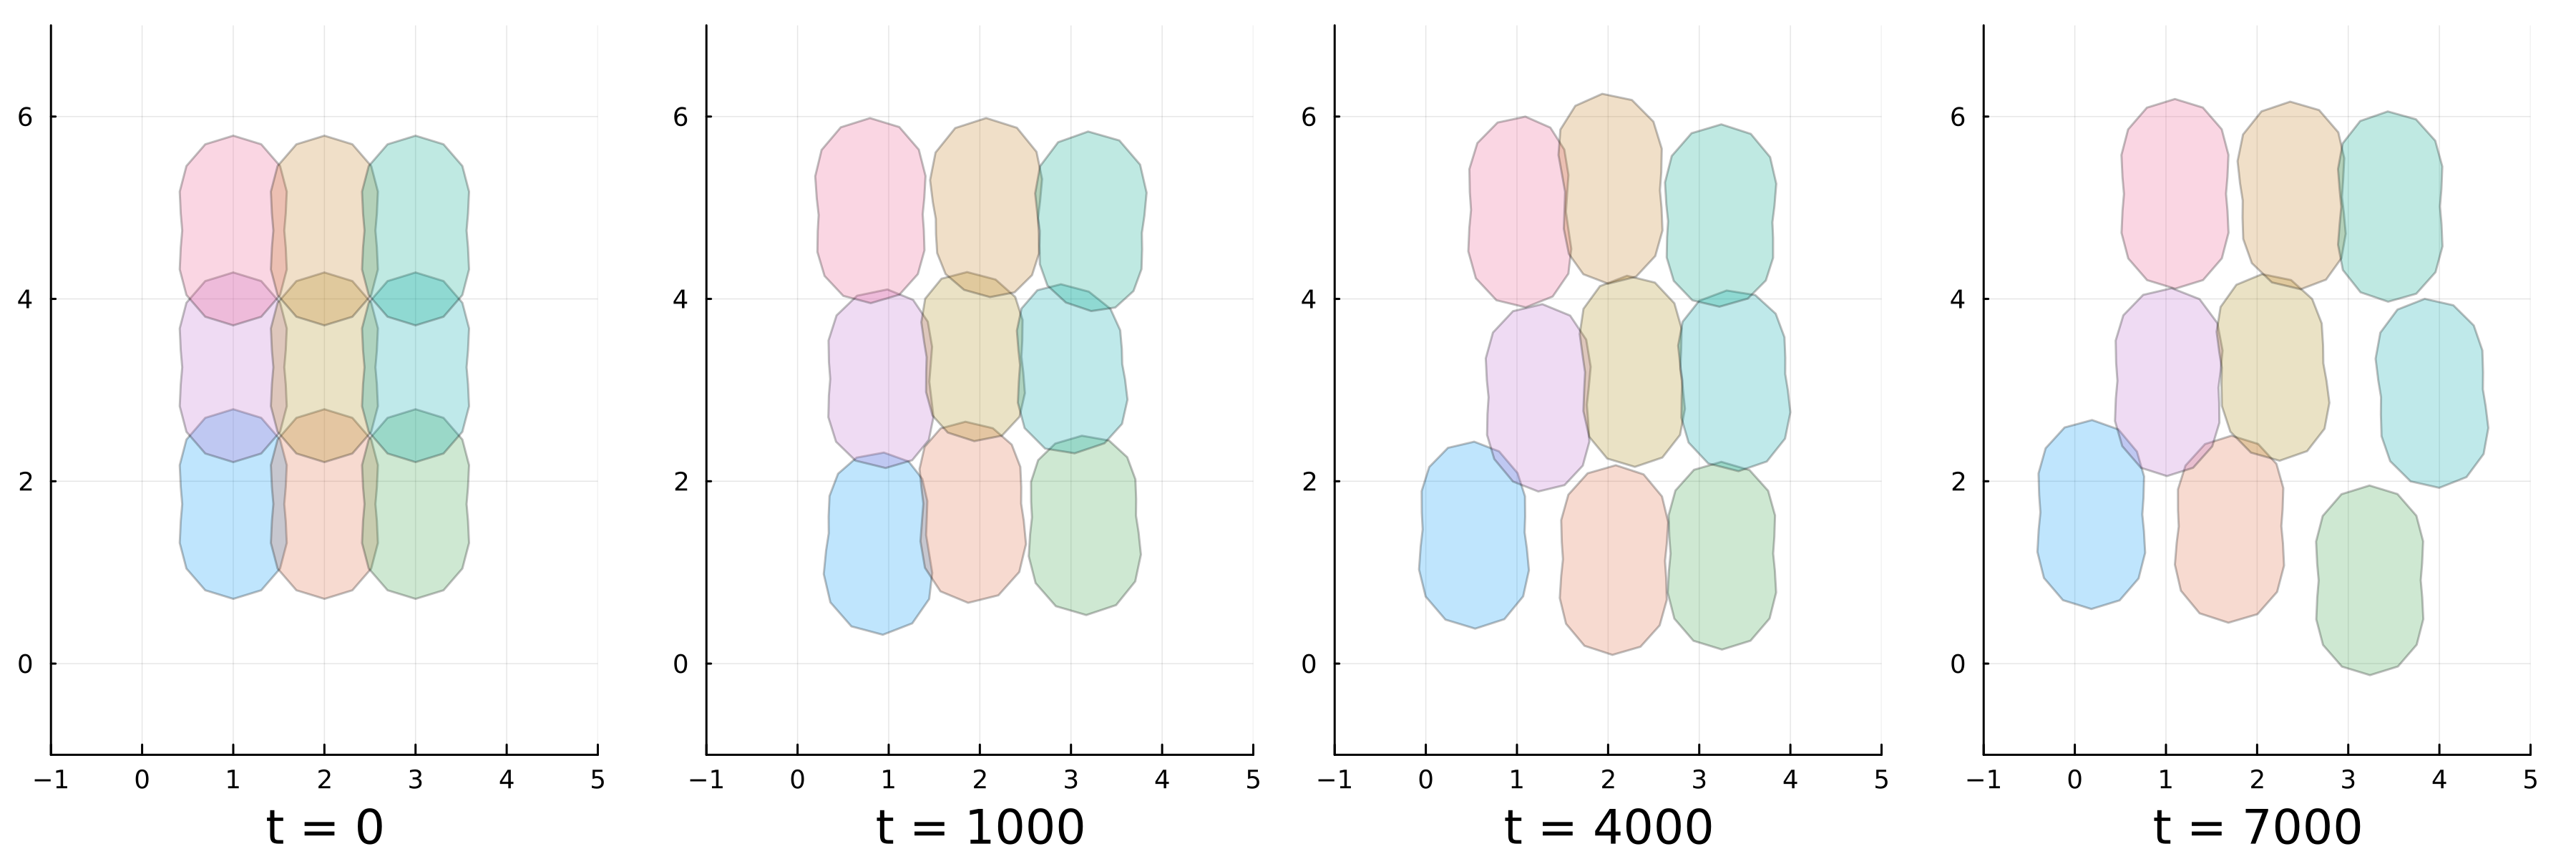
\includegraphics[width=15cm]{bachelors-thesis/forces/interaction/interaction_rescaled/interaction_rescaled.png}
		\caption{This figure shows different plots of a solution to the explained SDE \eqref{eq:interaction2} with the rescaled force configuration. We can see the cells at the times $t \in \{ 0, 1000, 4000, 7000\}$. }
		\label{fig:interaction_rescaled}
	\end{center}
\end{figure}

The \textbf{result of the bachelor's thesis} is a serviceable dynamic with interactions of an entire cellular system.

\newpage
\subsection*{Outlook of bachelor's thesis}
In \cite{Bruna2023} Bruna, Chapman and Schmidtchen studied a macroscopic model for Brownian hard needles. Similar to the hard sphere model in the paper \cite{Bruna2012} from the introduction, there are exclusion effects for the different needle particles. The authors managed to derive an effective PDE that describes the probability density $\rho(t,\vec{x}, \theta)$ of finding a needle with rotation $\theta$ at position $\vec{x}$ and time $t$. An interesting next step for the development of the theory in this thesis would be to derive an effective PDE for our energy dynamic model of the DF cells. \\

% \section*{Overview - Master's thesis }
The first task of the Master's thesis is to do a sanity check with the paper \cite{Bruna2012}. 
\begin{figure}[h!]
	\centering
	\hfill
	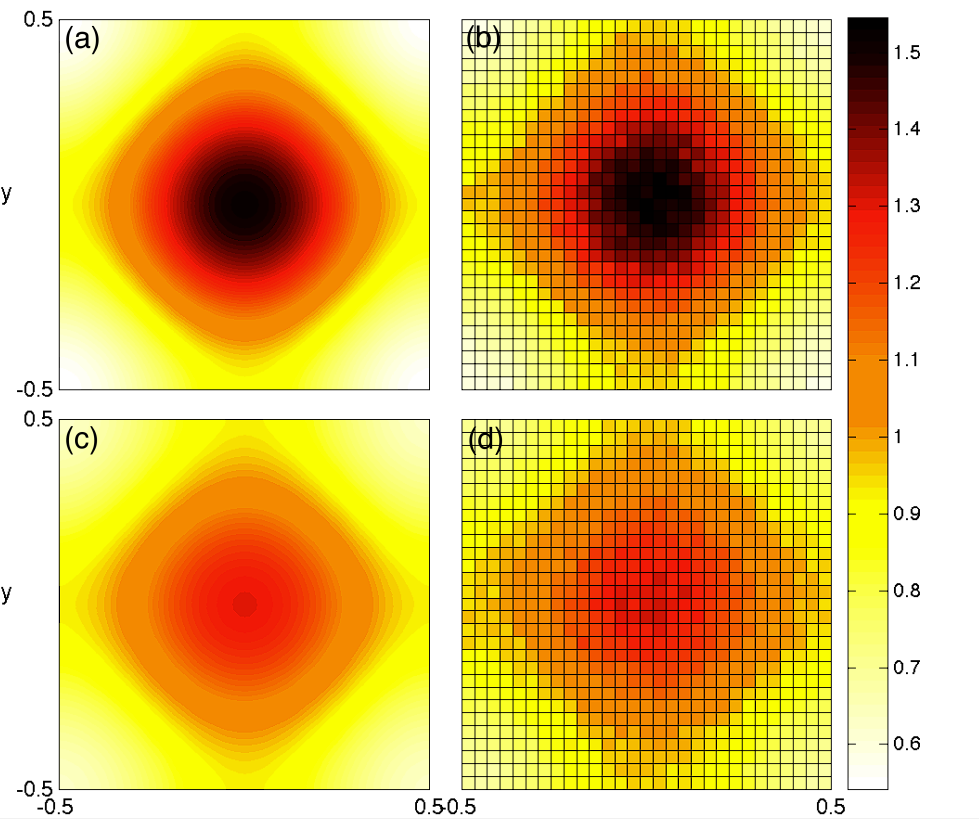
\includegraphics[width=\textwidth]{sanity-check/bruna12_theOriginal.png}
\end{figure}
Until now, we made 2 bigger simulations. We neglected the interior angle force, because it caused stability problems. 

\newpage
\subsection*{First big simulation}
Here is our most recent simulation parameters:
\begin{itemize}
    \item 16 cells are spawned at a fixes 4x4 initial state 
    \item 40 wall points per cell 
    \item Diffusitivity constant $D=5.0$
    \item bachelor scalings, but wihtout interior angle force for better stability
    \item $time interval = [0, 100]$
    \item $time step size = 2^{-8}$
    \item used bachelor overlap 
    \item 300 simulations ran 
    \item $grid = [-5,5]^2$ with discretisation step size $\delta x = 0.25$
\end{itemize}

% FIGURE OF FIRST BIG SIMULATION
\begin{figure}[h!]
	\centering
	\begin{subfigure}{0.4\textwidth}
		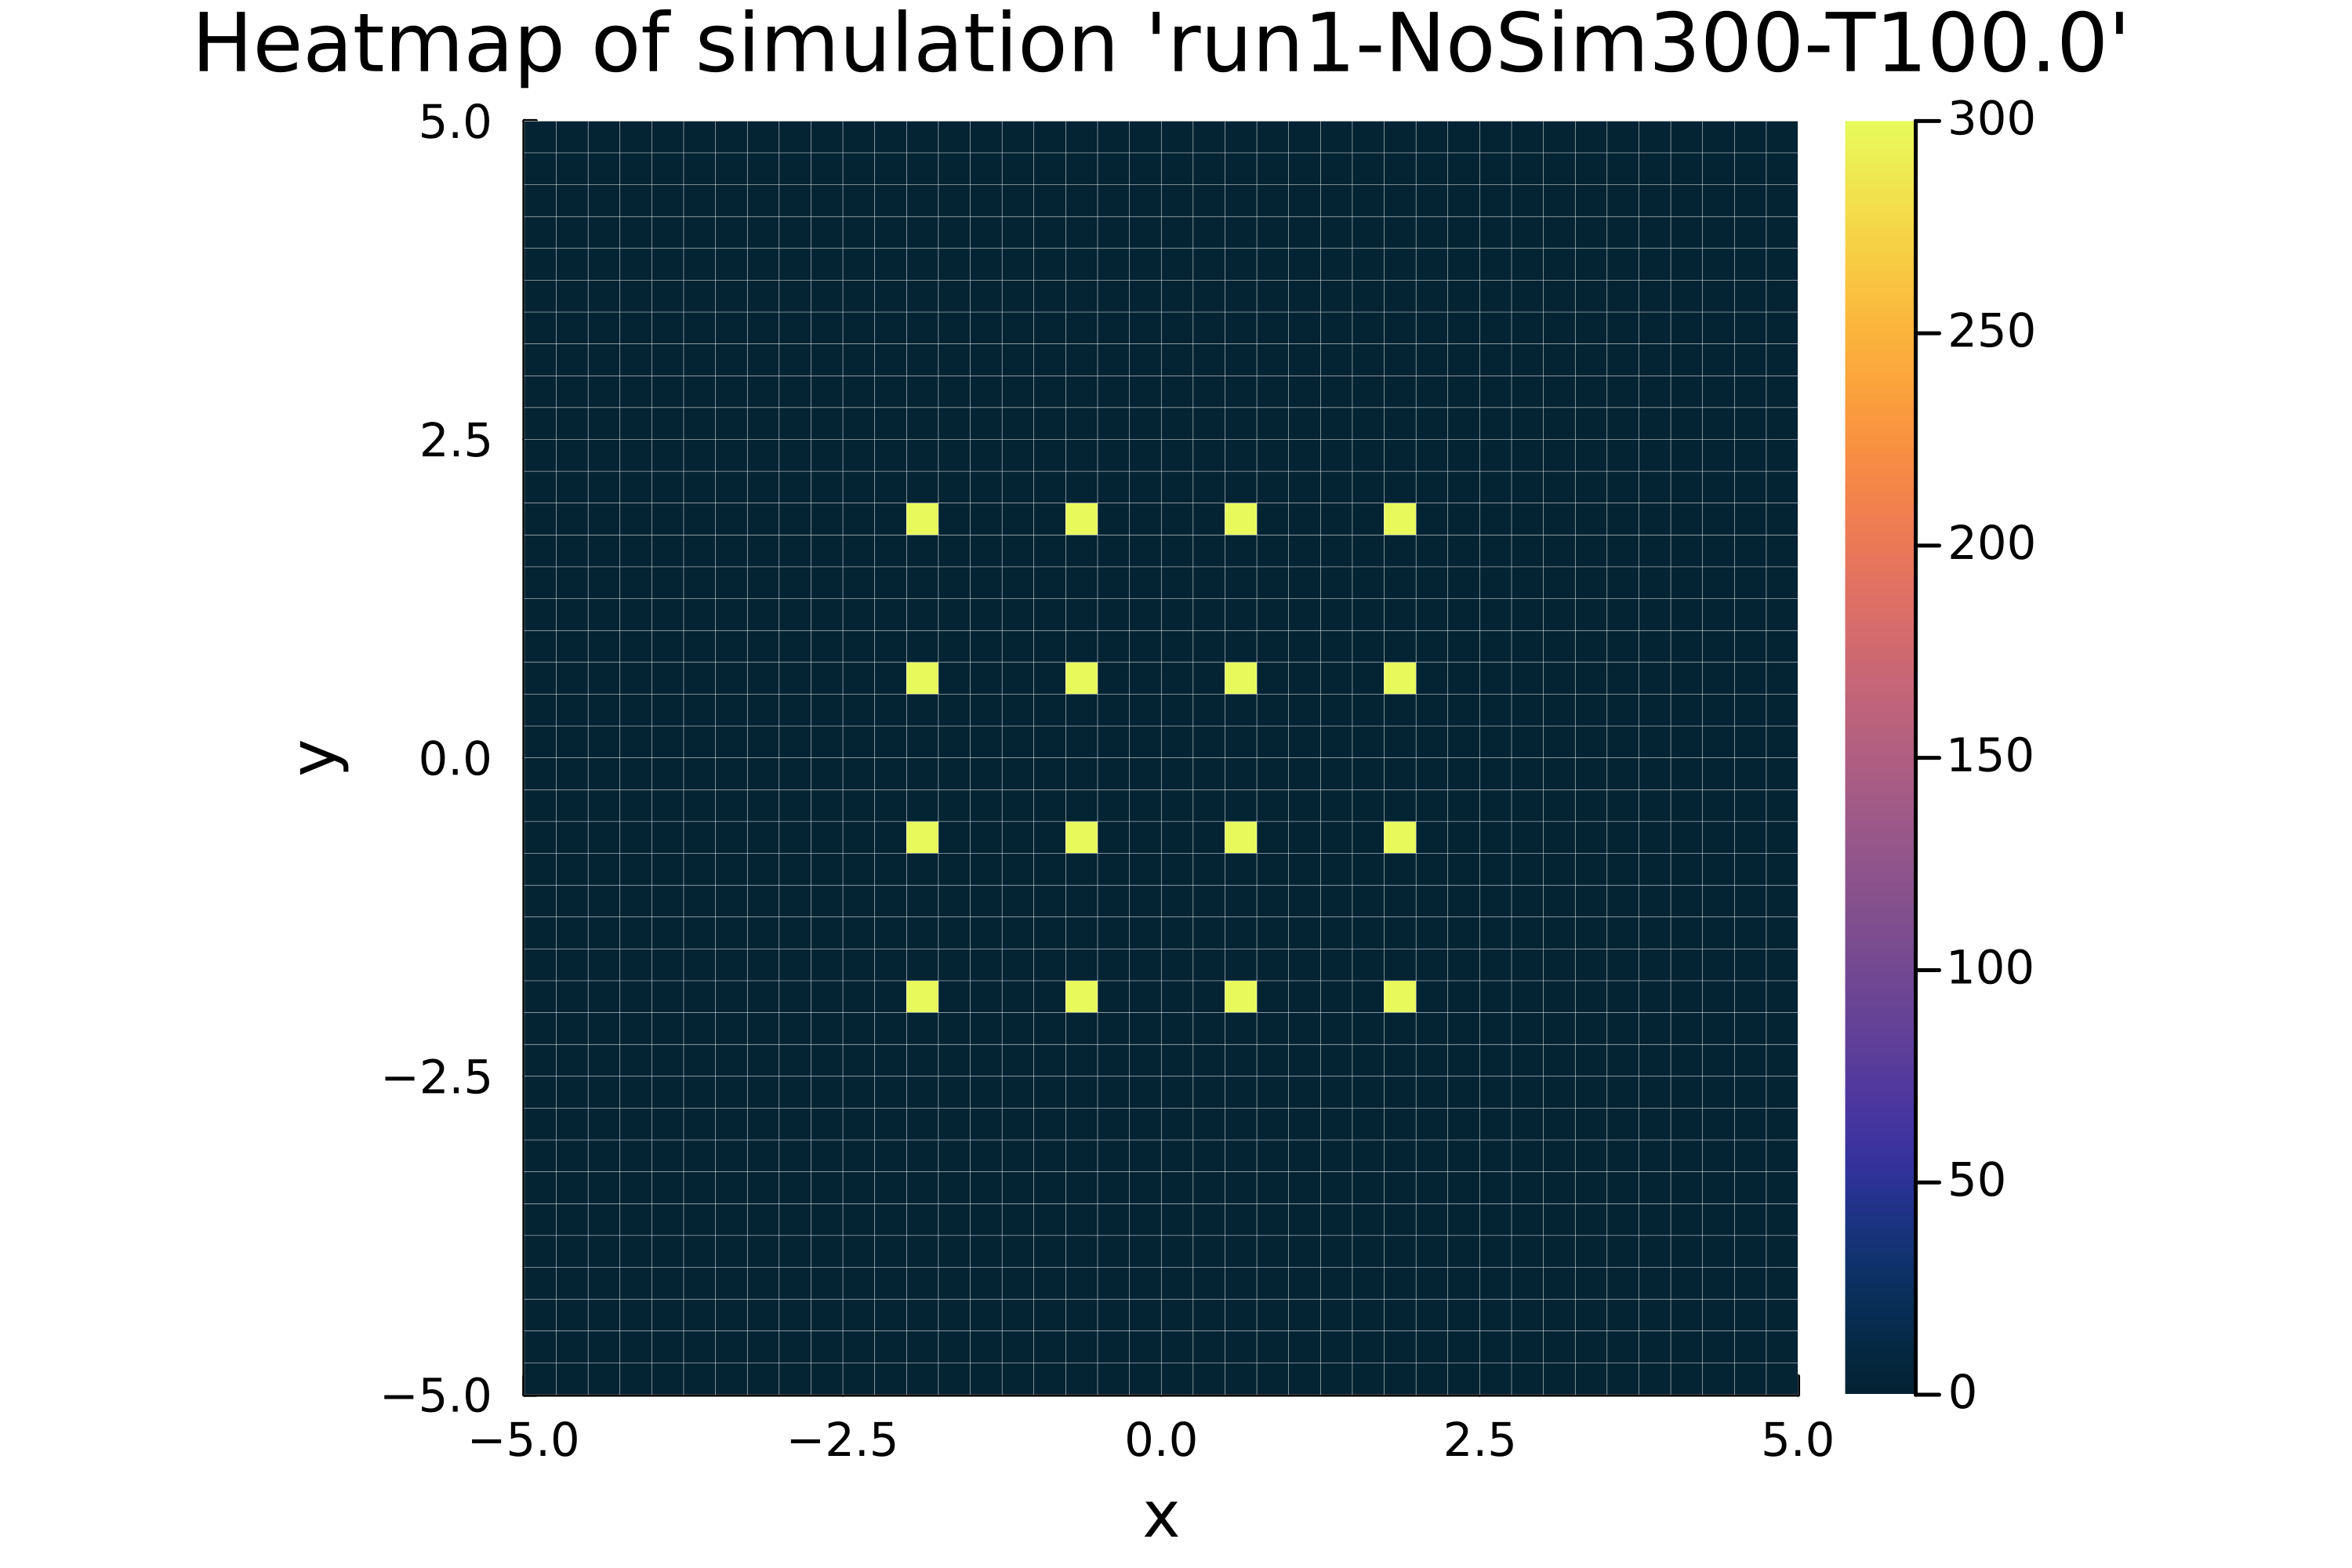
\includegraphics[width=\textwidth]{sanity-check/Heatmap-run1-NoSim300-T100.0/heatmaps/heatmap-run1-NoSim300-T100.0-sampleTime0001.png}
	\end{subfigure}
	\hfill
	\begin{subfigure}{0.4\textwidth}
		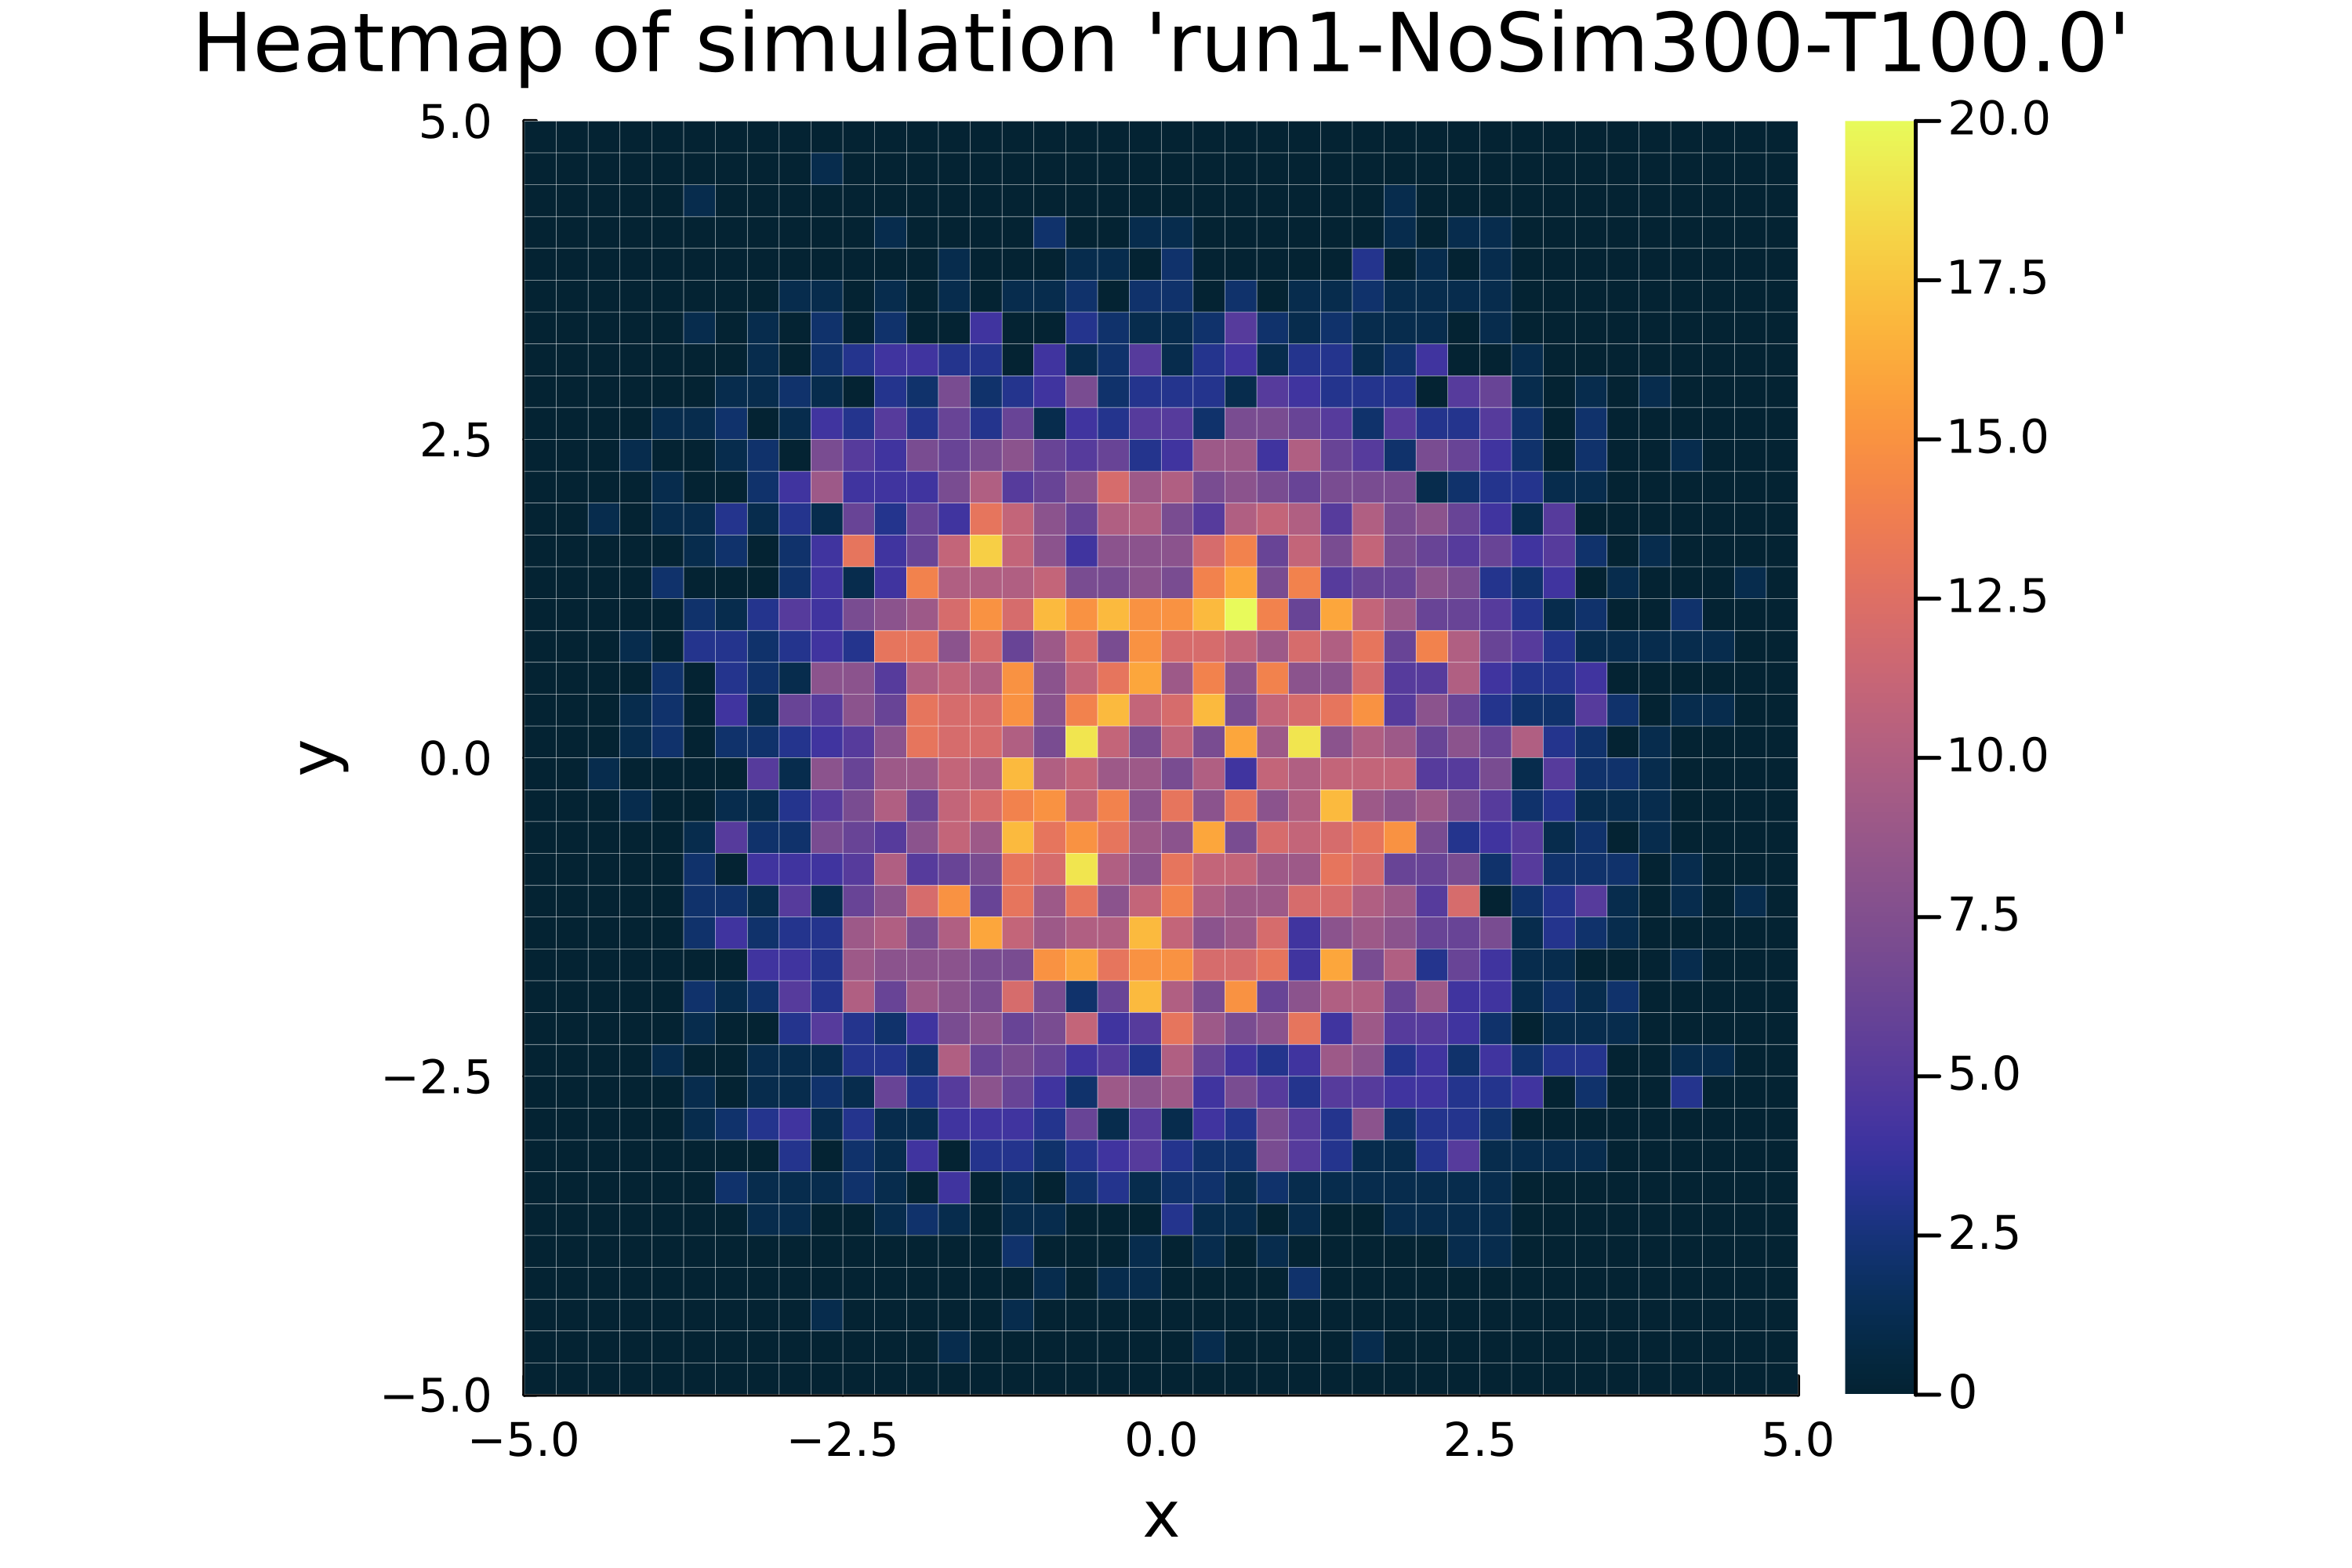
\includegraphics[width=\textwidth]{sanity-check/Heatmap-run1-NoSim300-T100.0/heatmaps/heatmap-run1-NoSim300-T100.0-sampleTime5000.png}
	\end{subfigure}
	\hfill
	\begin{subfigure}{0.4\textwidth}
		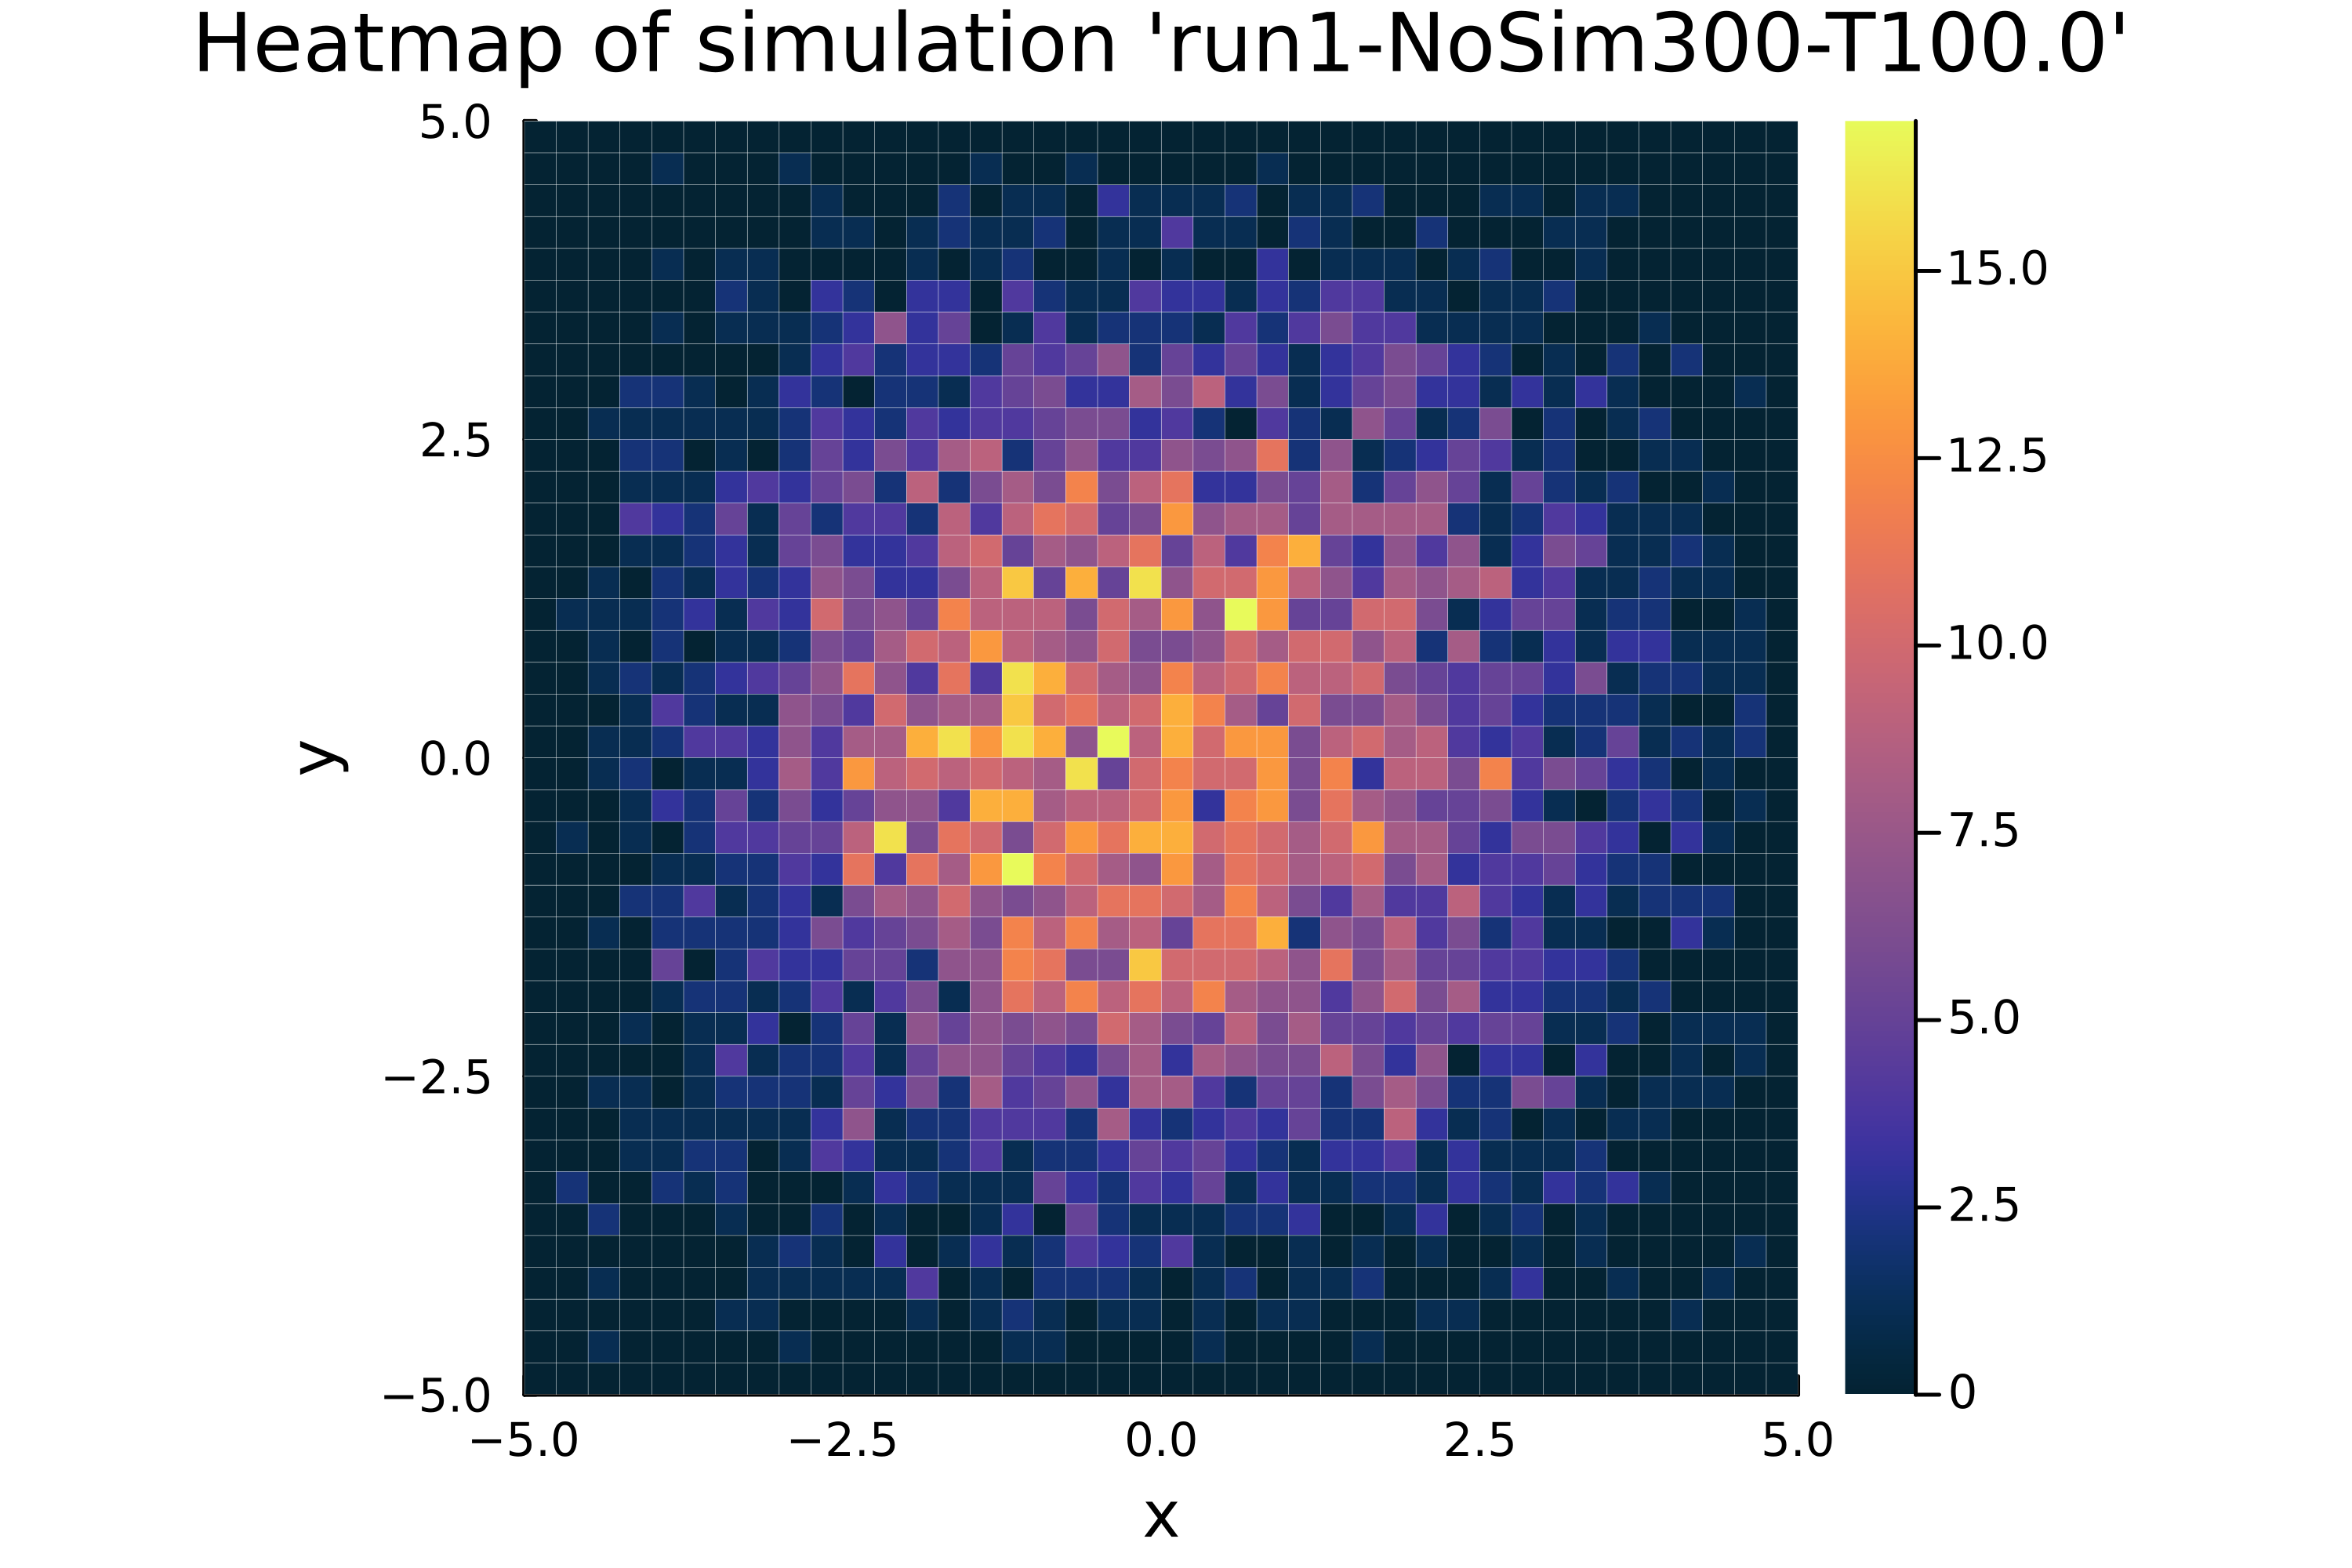
\includegraphics[width=\textwidth]{sanity-check/Heatmap-run1-NoSim300-T100.0/heatmaps/heatmap-run1-NoSim300-T100.0-sampleTime10000.png}
	\end{subfigure}\hfill
	\begin{subfigure}{0.4\textwidth}
		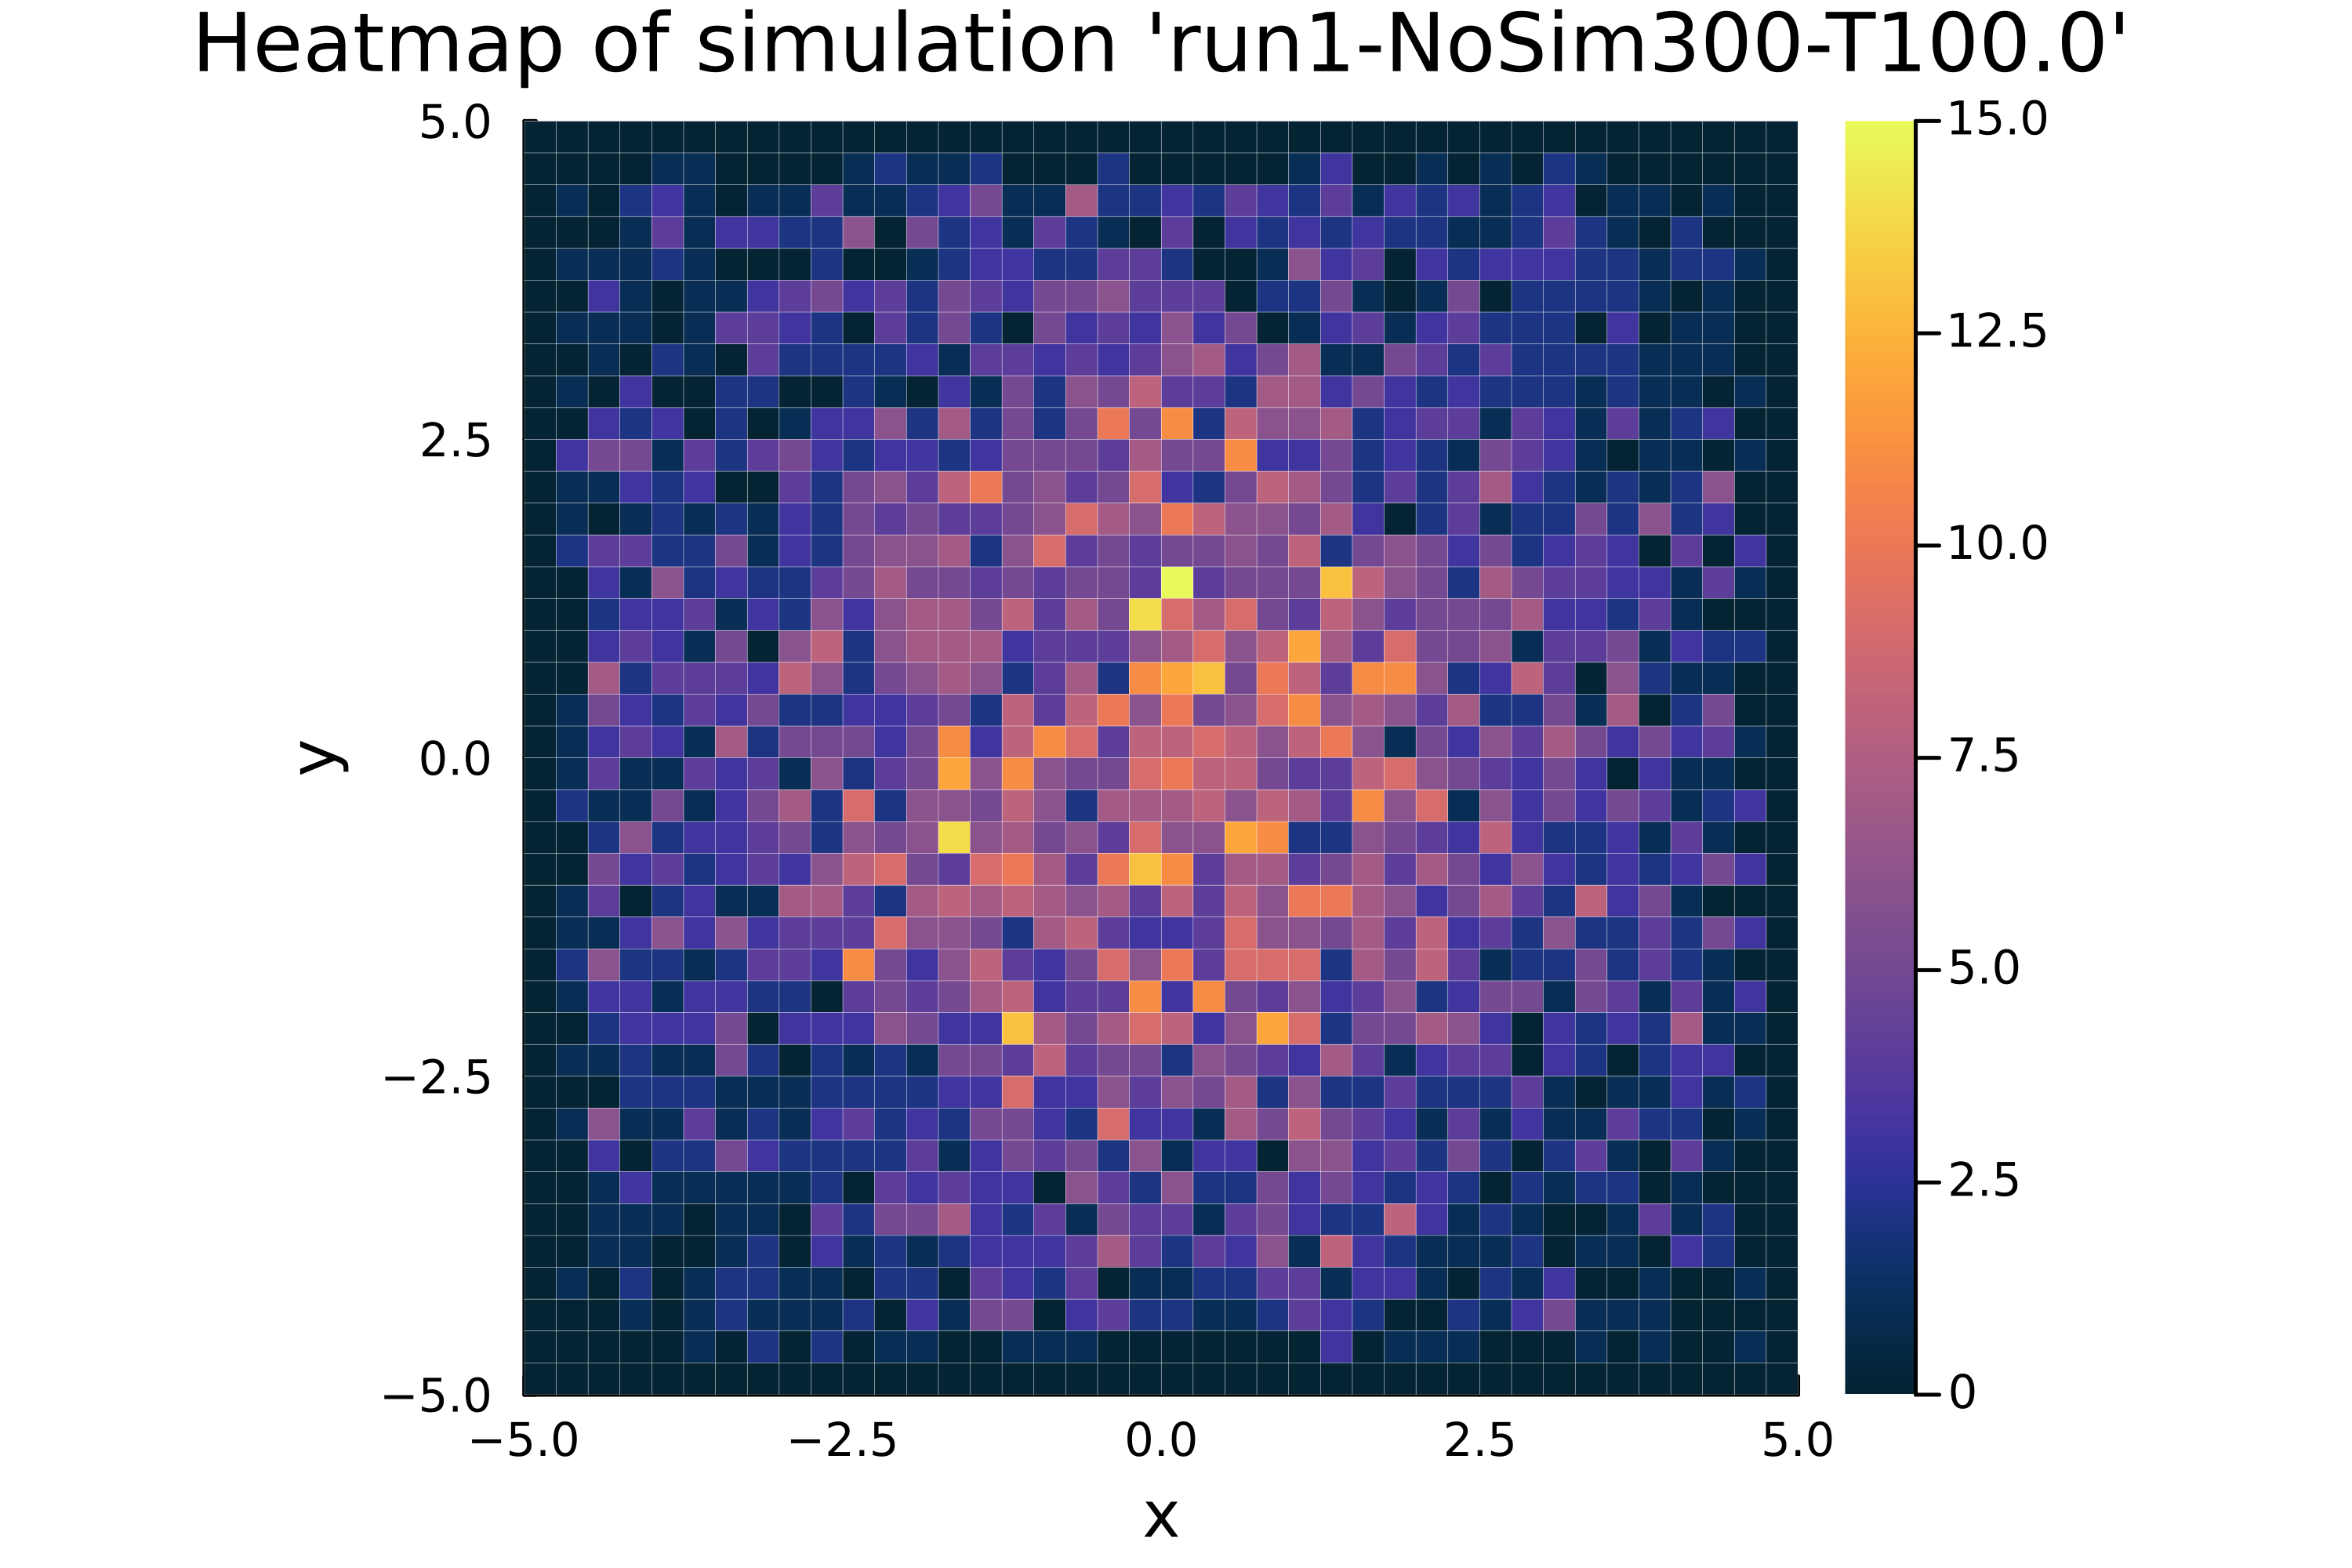
\includegraphics[width=\textwidth]{sanity-check/Heatmap-run1-NoSim300-T100.0/heatmaps/heatmap-run1-NoSim300-T100.0-sampleTime25000.png}
	\end{subfigure}
	\label{fig:model_illus}
\end{figure}


\newpage
\subsection*{Second big simulation}
Here is our most recent simulation parameters:
\begin{itemize}
    \item 100 cells are spawned normally distributed at the domain but without overlaps  
    \item 20 wall points per cell 
    \item Diffusitivity constant $D=100.0$
    \item bachelor scalings, but wihtout interior angle force for better stability
    \item $time interval = (0.0, 0.05)$
    \item $time step size = 10^{-4} = 0.0001$
    \item used radius billiard overlap 
    \item 3 simulations ran 
    \item $grid = [-5,5]^2$ with discretisation step size $\delta x = 0.25$
\end{itemize}

% FIGURE OF SECOND BIG SIMULATION
\begin{figure}[h!]
	\centering
	\begin{subfigure}{0.4\textwidth}
		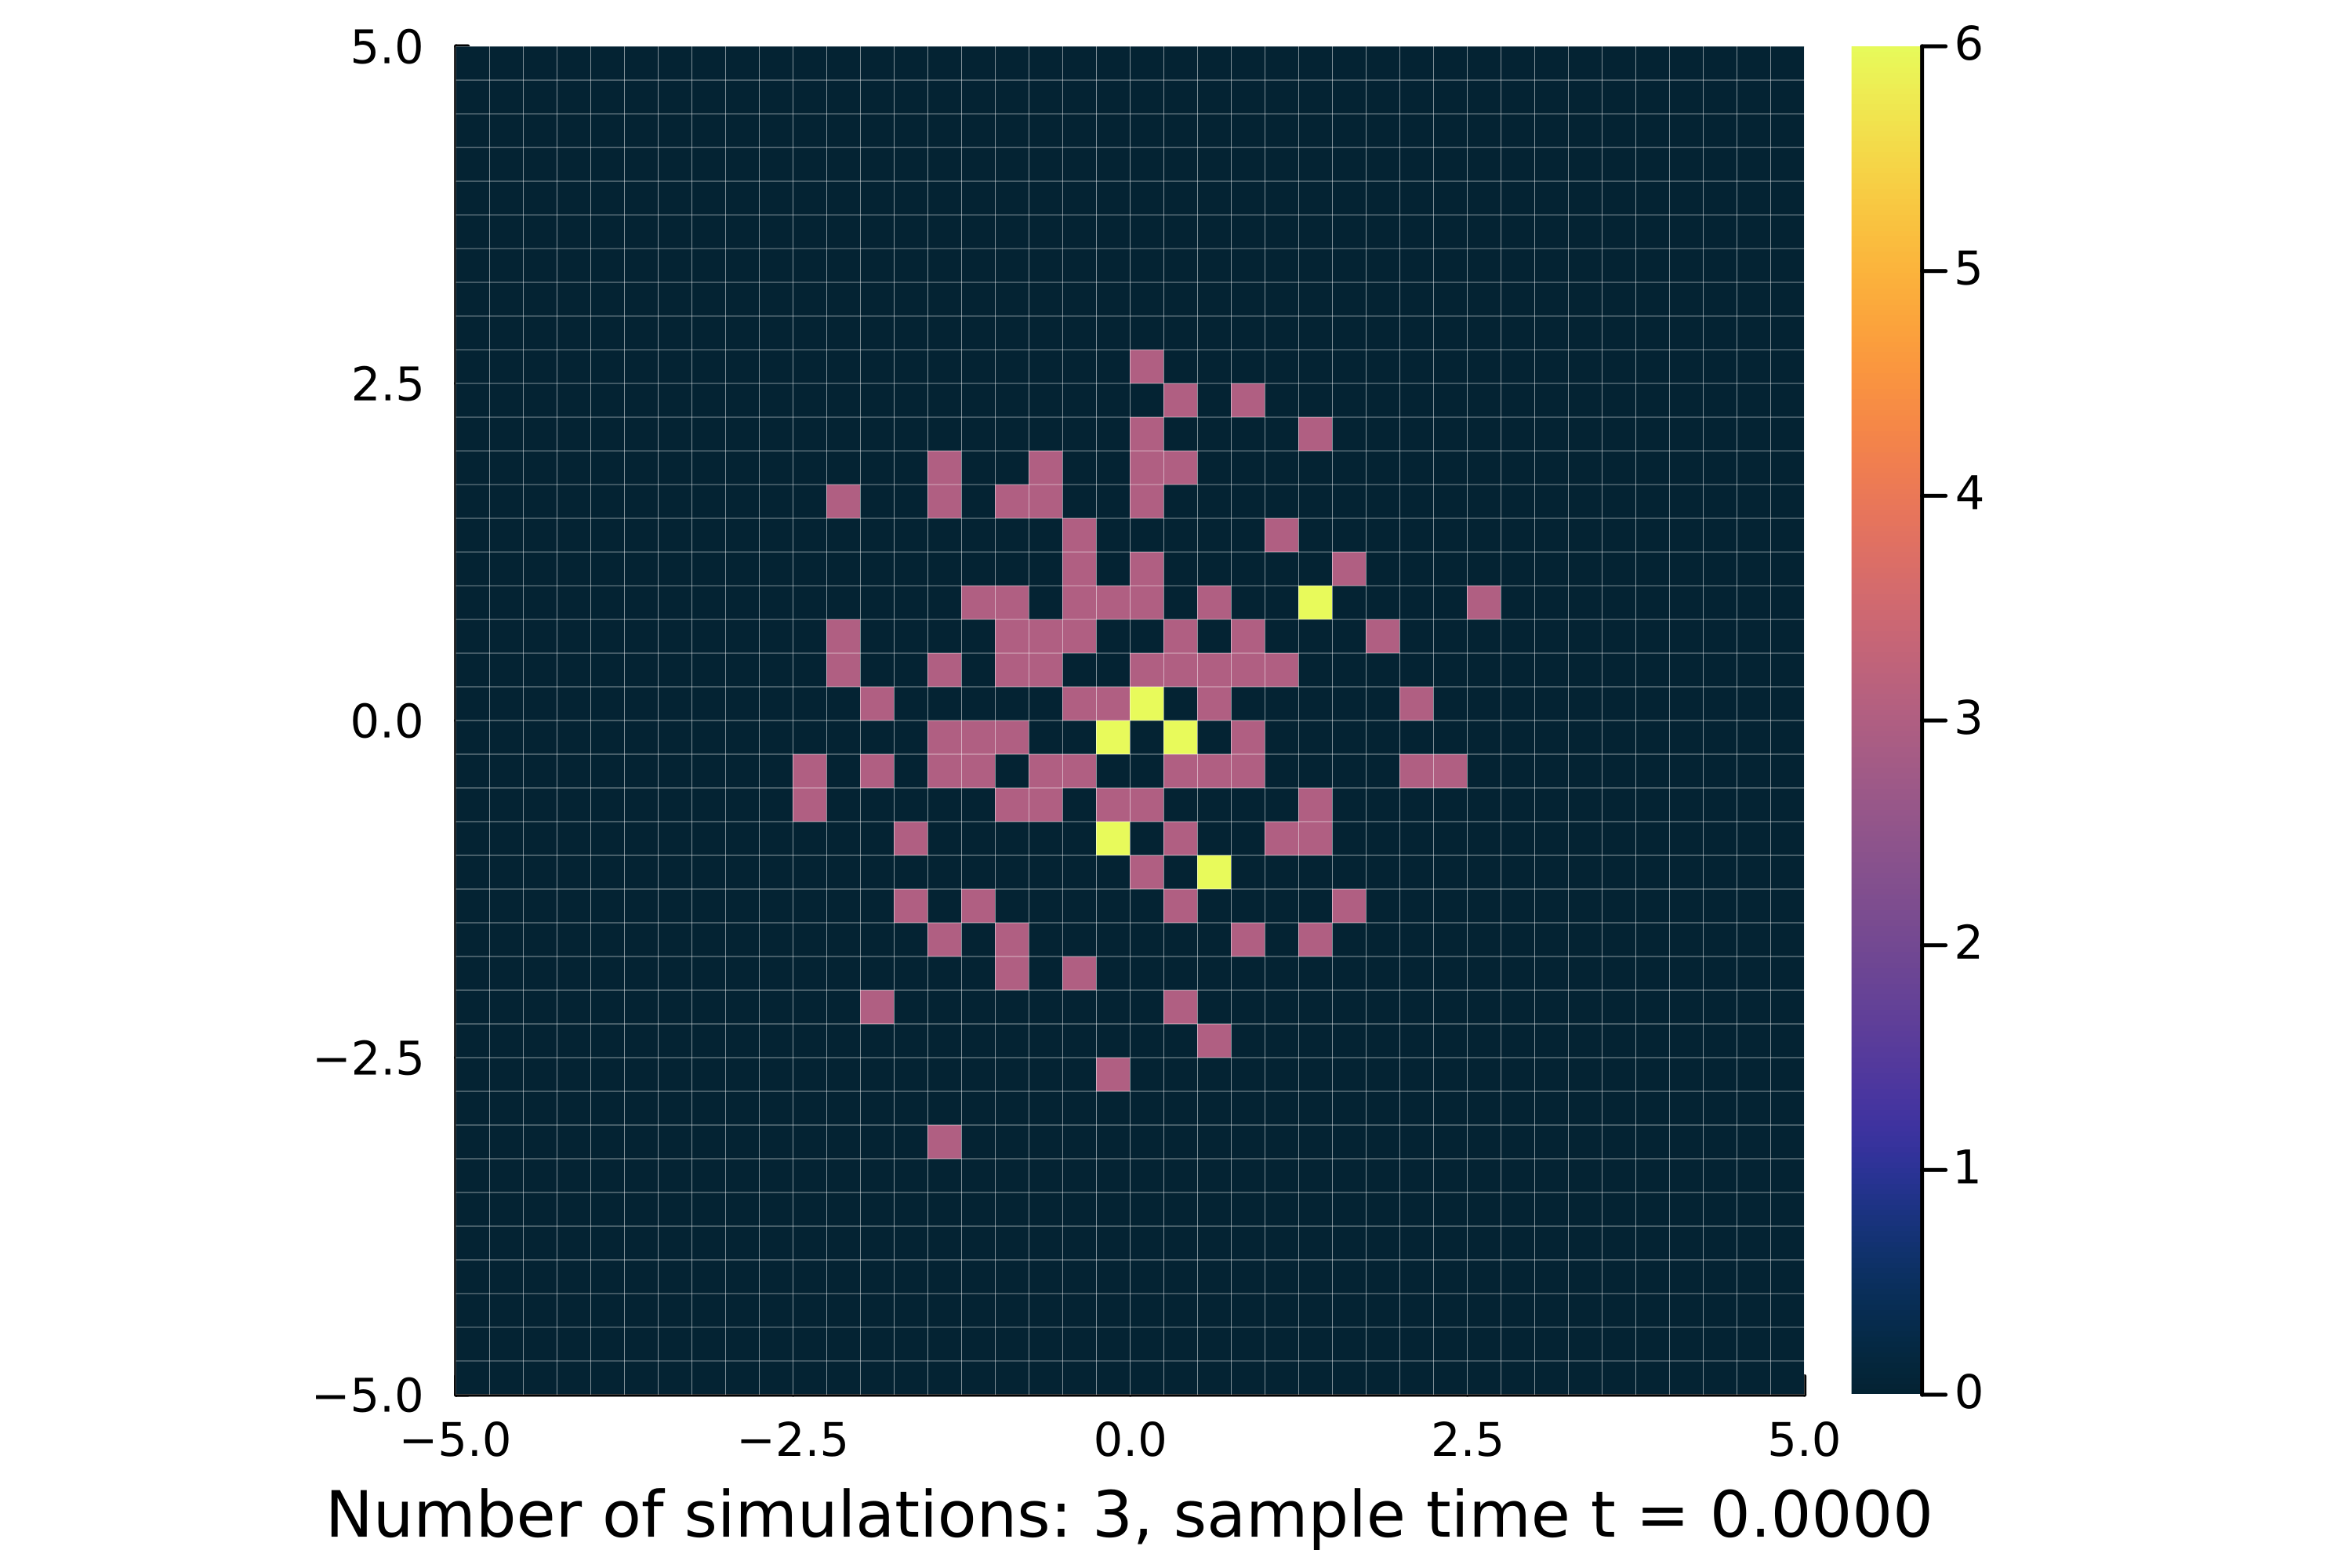
\includegraphics[width=\textwidth]{sanity-check/imitate-hardsphere-bruna-test1/heatmaps/heatmap-imitate-hardsphere-bruna-test1-sampleTime0.0.png}
	\end{subfigure}
	\hfill
	\begin{subfigure}{0.4\textwidth}
		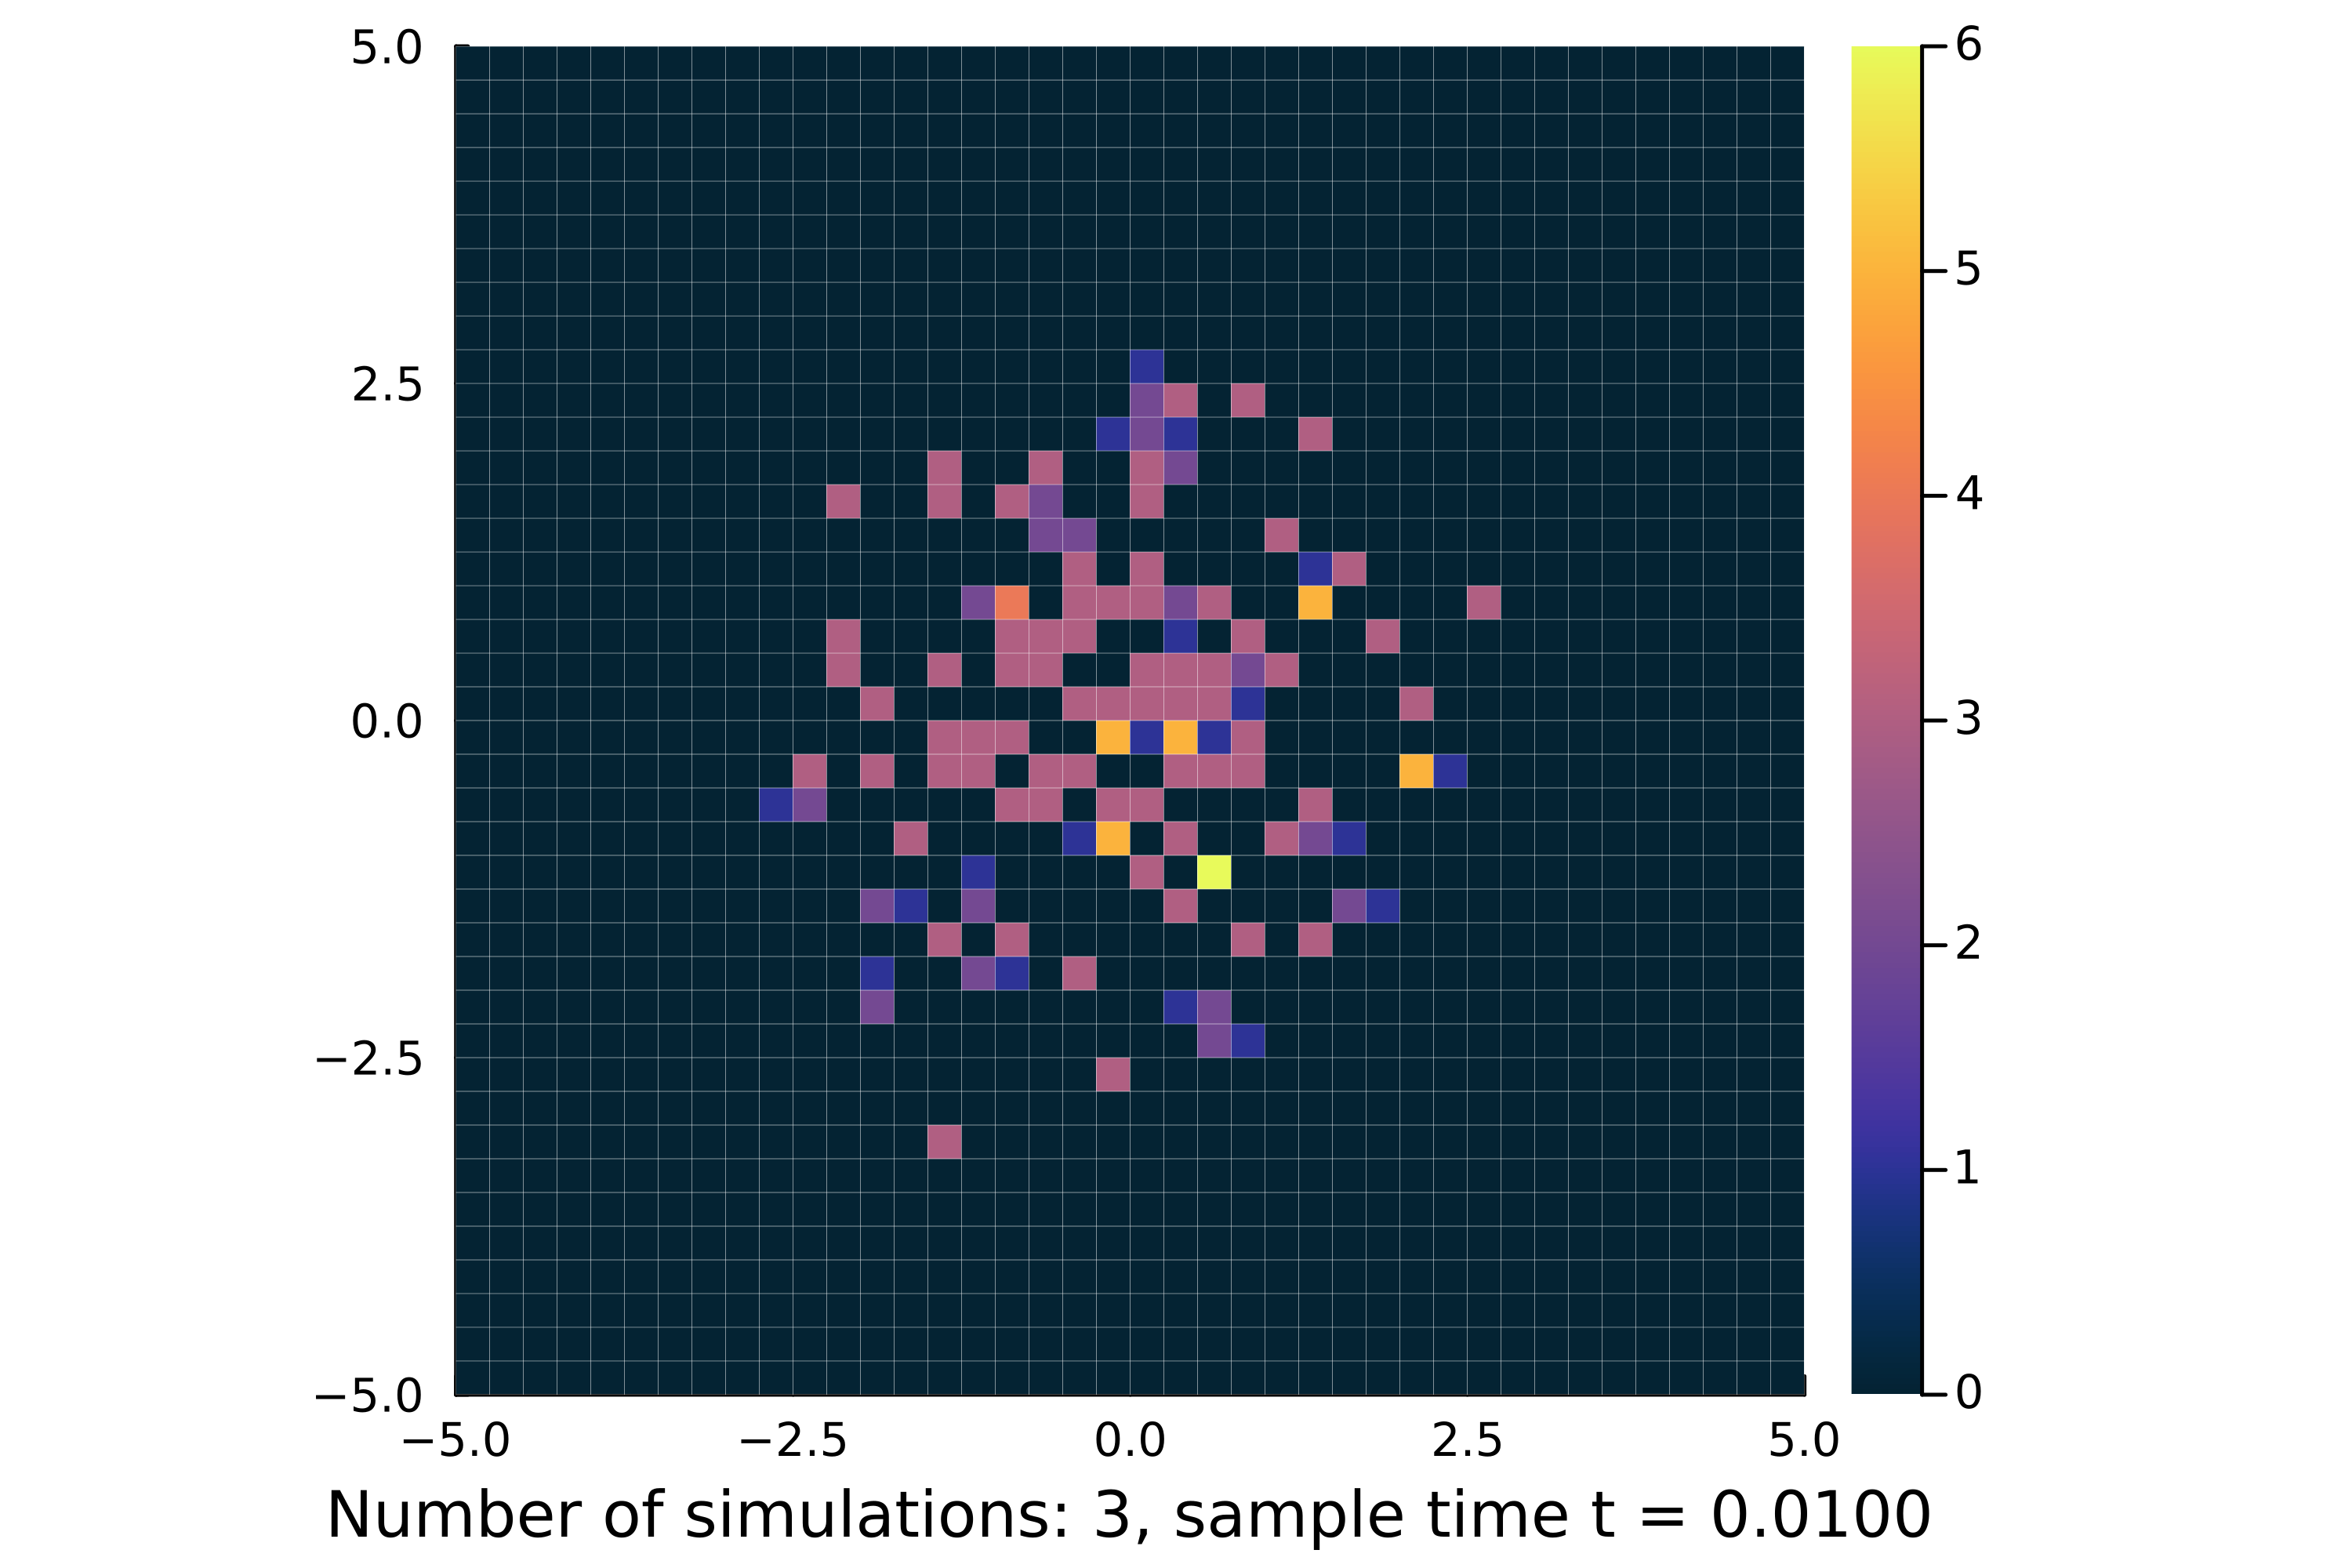
\includegraphics[width=\textwidth]{sanity-check/imitate-hardsphere-bruna-test1/heatmaps/heatmap-imitate-hardsphere-bruna-test1-sampleTime0.01.png}
	\end{subfigure}
	\hfill
	\begin{subfigure}{0.4\textwidth}
		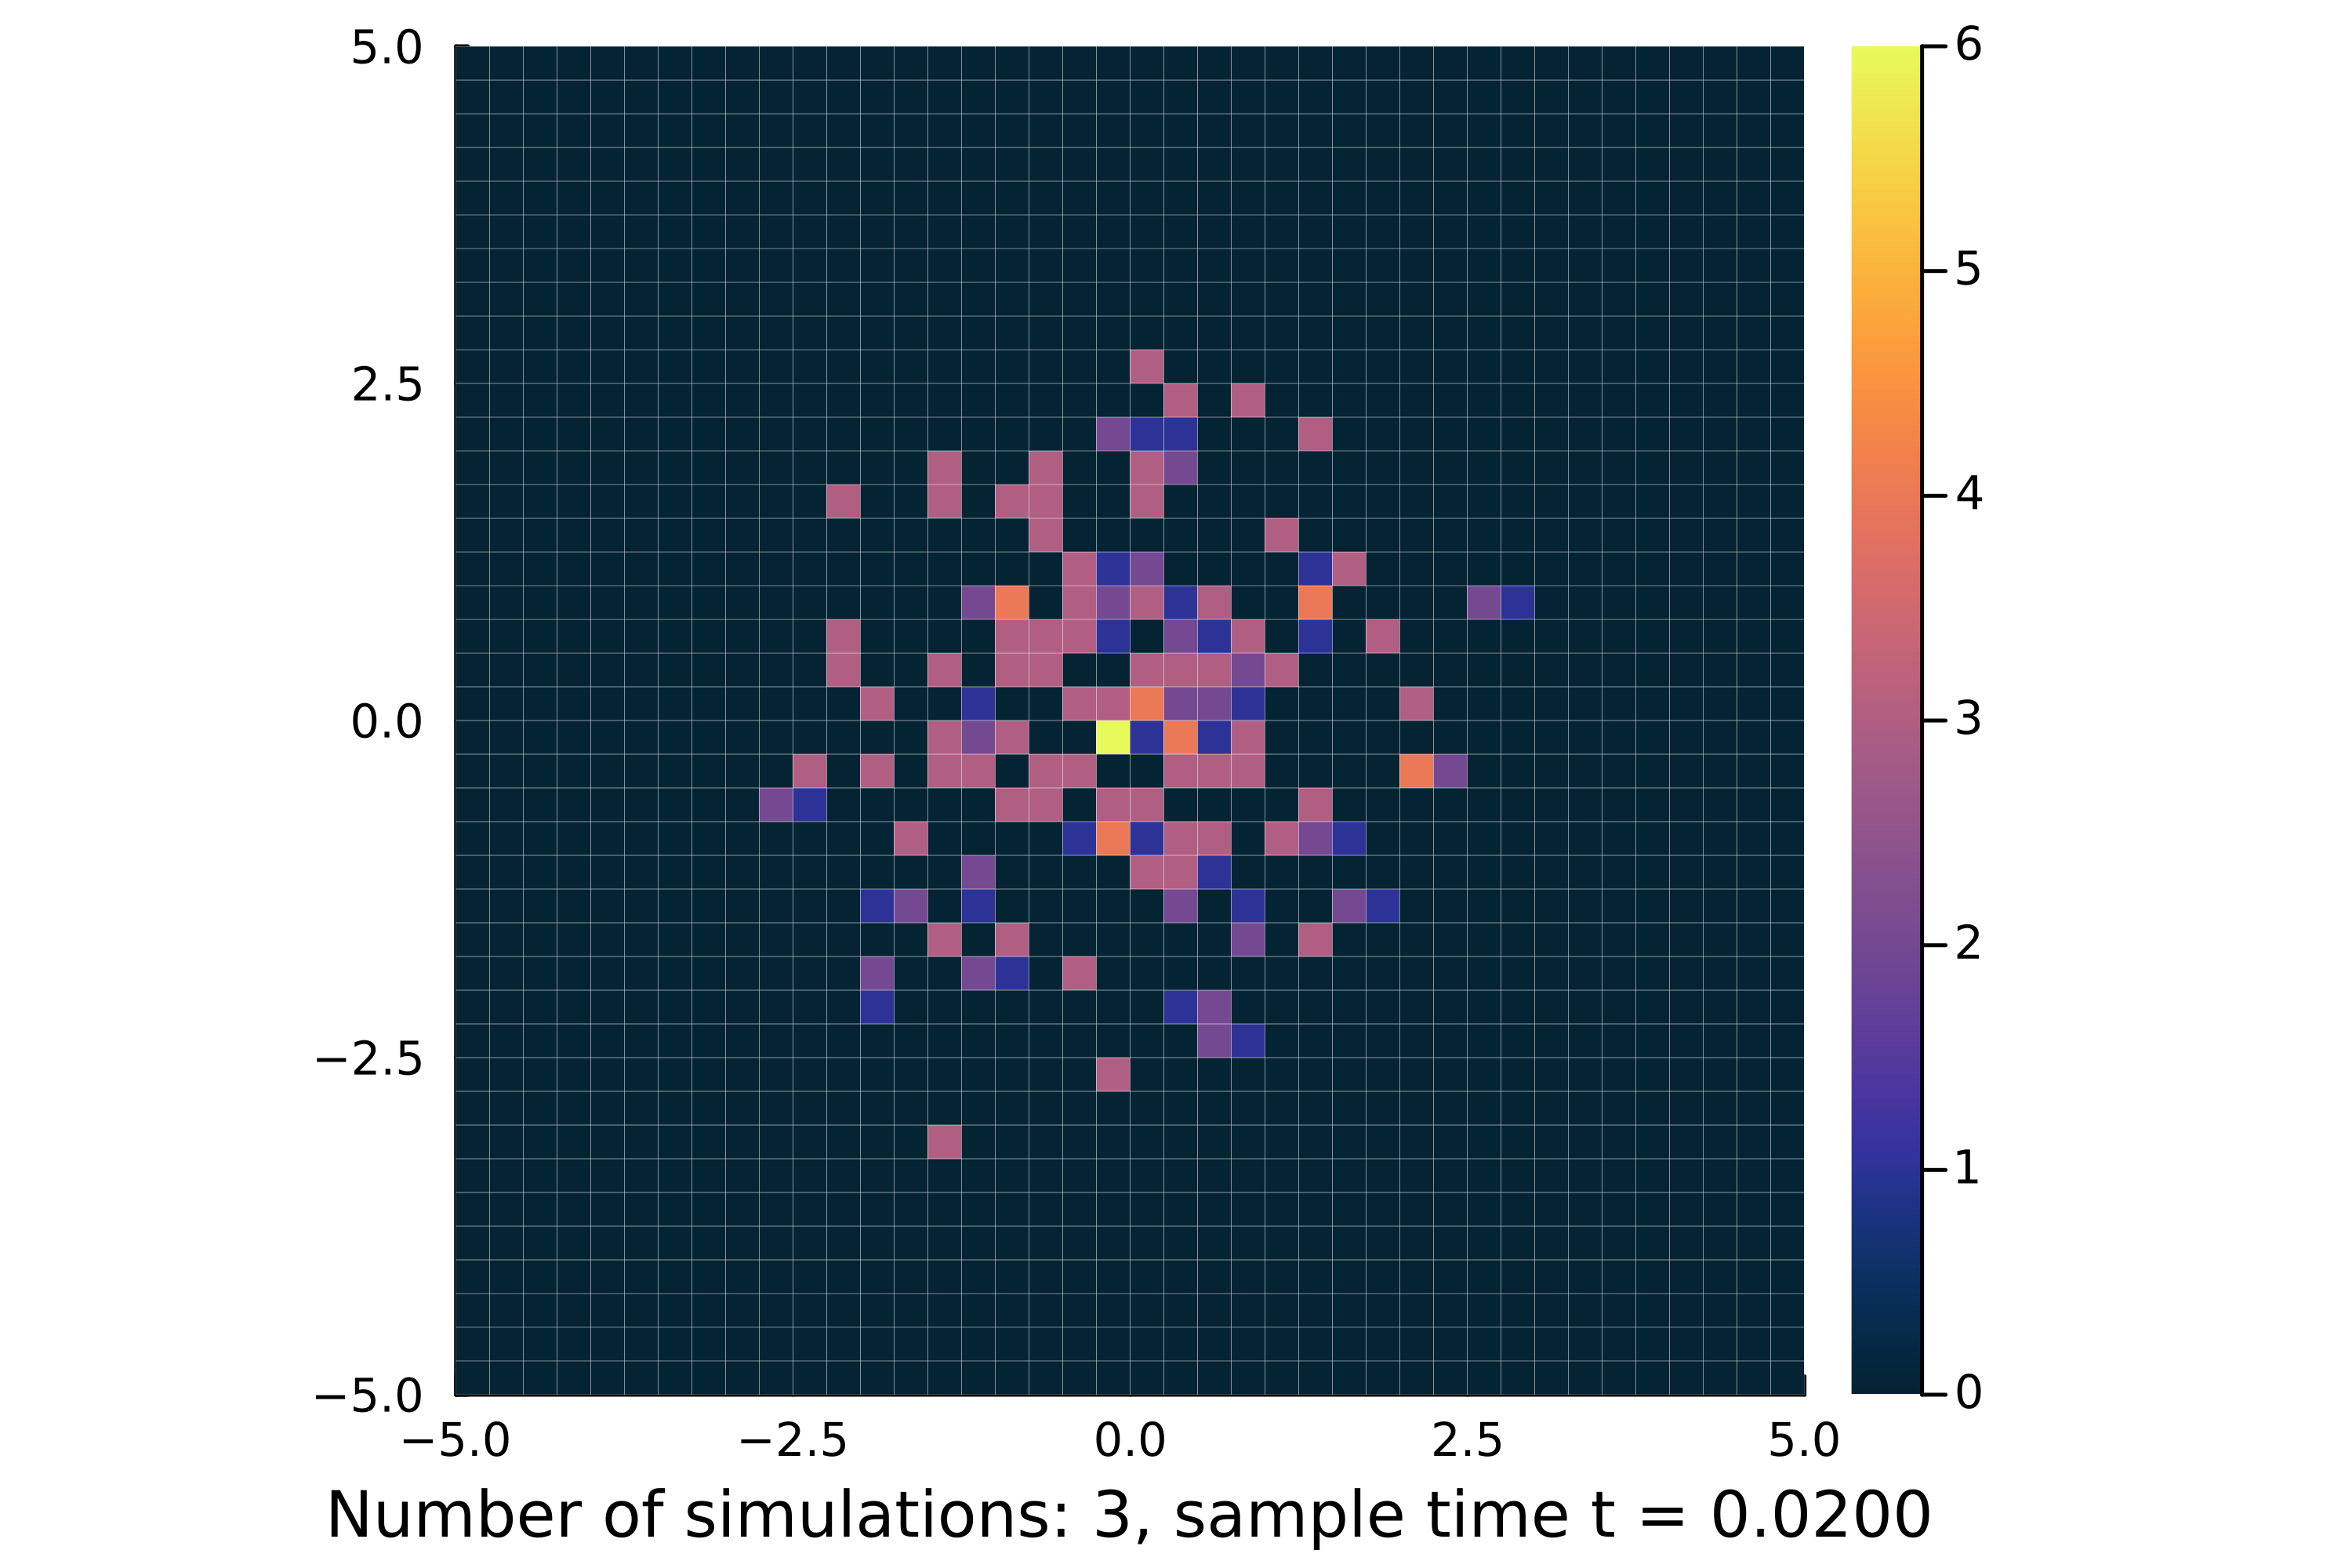
\includegraphics[width=\textwidth]{sanity-check/imitate-hardsphere-bruna-test1/heatmaps/heatmap-imitate-hardsphere-bruna-test1-sampleTime0.02.png}
	\end{subfigure}\hfill
	\begin{subfigure}{0.4\textwidth}
		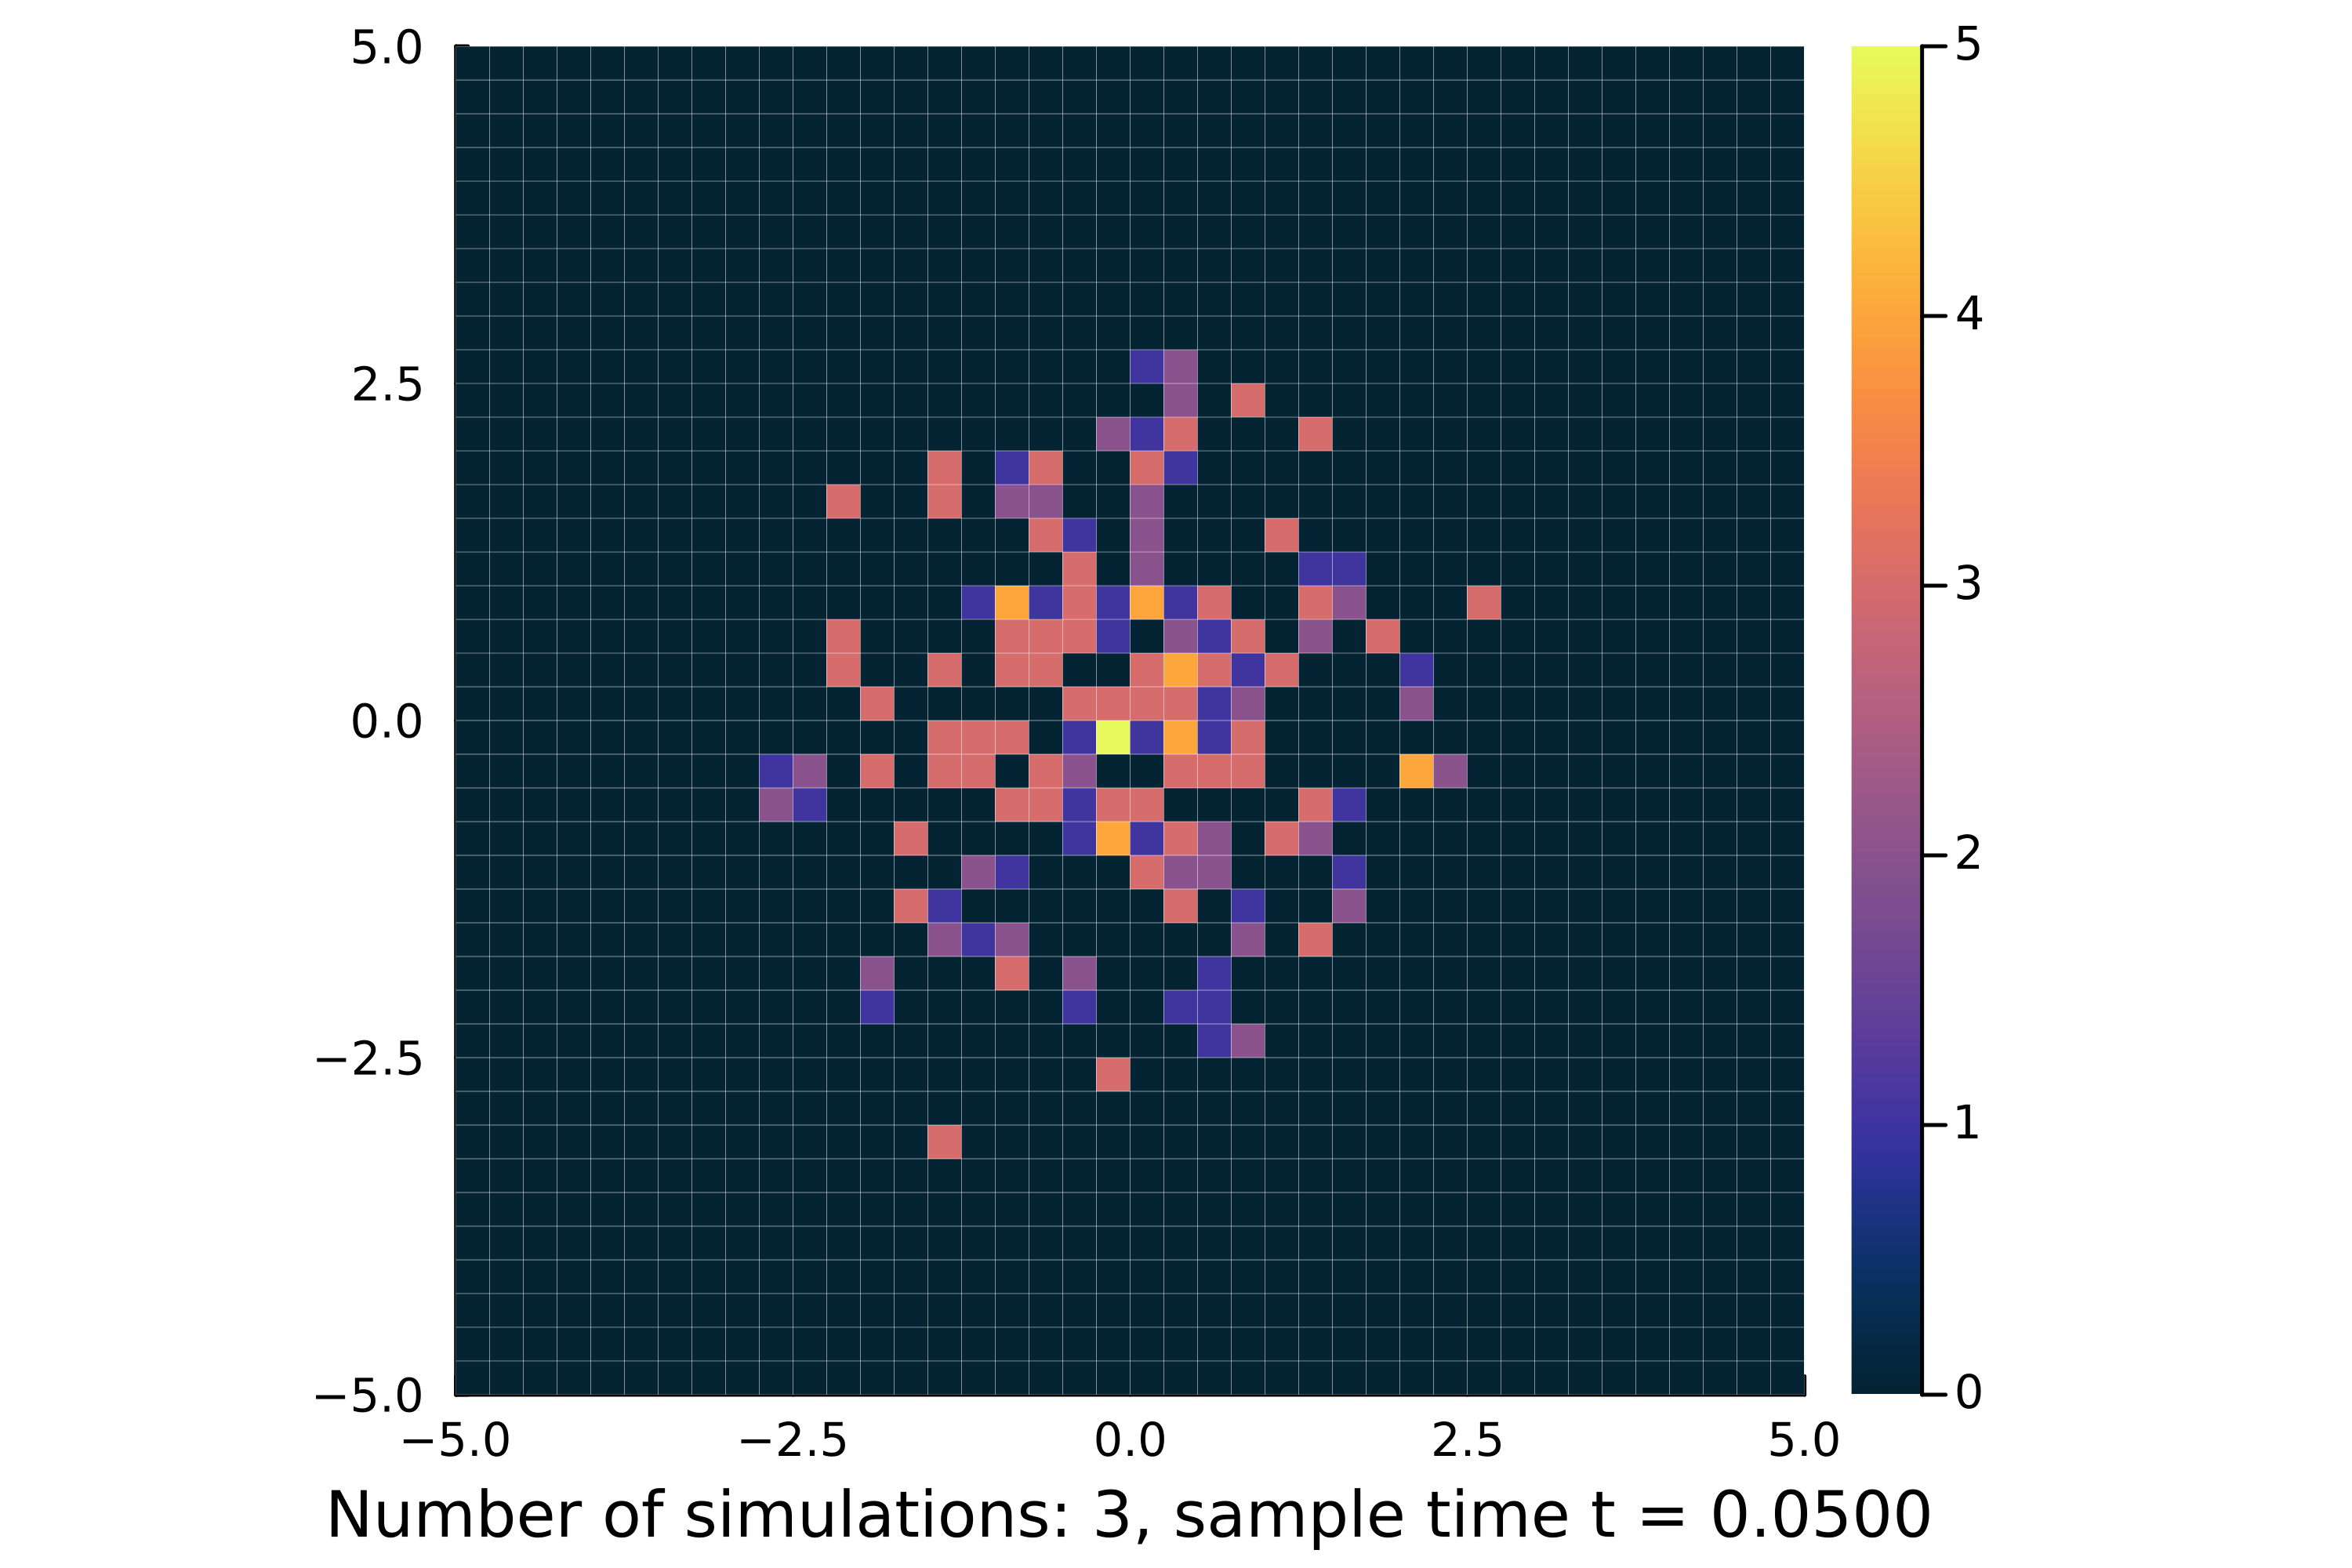
\includegraphics[width=\textwidth]{sanity-check/imitate-hardsphere-bruna-test1/heatmaps/heatmap-imitate-hardsphere-bruna-test1-sampleTime0.05.png}
	\end{subfigure}
	\label{fig:model_illus}
\end{figure}

\newpage
\subsection*{Overlaps}
\textbf{bachelor overlap (l 441 in energies.jl)}
\textbf{billiard overlap (l 474 in energies.jl)}
\textbf{combination of first 2 overlap  (l 539 in energies.jl)}
\textbf{radiusOverlapForceCells overlap (l 506 in energies.jl)}

\newpage
\subsection*{Next Steps}
\begin{itemize}
	\item Recreate chapman12 heatmap 
	
	\item 
	$
	initial condition: X' = \sqrt{10} X + 1, \quad \text{where } X \sim N(0,1) \\
	NoCells' = x (NoCells = 400) \\
	radius' = y (radius = 0.005) \\
	$AND ALSO$ radius' = 0 $ and without interaction [other parameters the same?] $
	time = [0.00,0.05], \delta t = 10^{-5} \\
	NoSimulations = 10^4 \\
	$Maybe run on linux work station in Z21$
	$
	\item parallelize code 
	\item use same color grading as in chapman12 (name?)

\end{itemize} 



% \section{Introduction}
%%% TODO: mention all figures in text 
%%% TODO: add motiviation for cell diffusion models from real world applications 
% from bridge paper:
Collective cell migration represents a fundamental process underpinning various biological phenomena, including embryonic development, tissue regeneration, wound healing, and the invasive potential of certain cancers. 
The collective nature of cell movement has been acknowledged for over a century, with early observations recognising its importance in developmental and regenerative processes~\cite{alert2020, holmes1914, herrick1932, vaughan1966}. 
However, the underlying mechanisms driving this coordinated behavior remained contentious, with competing hypotheses suggesting roles for pressure~\cite{herrick1932}, surface tension~\cite{alert2020}, or active forces generated by leading cells~\cite{holmes1914}. \\
Following a period where research emphasis shifted towards molecular and genetic details, the field has witnessed a resurgence of interest in understanding the physical principles governing collective cell migration. 
This revival is largely attributed to recent advances in experimental techniques~\cite{roca2017, du2005, trepat2009}, enabling direct measurements of mechanical forces exerted by cells, and the development of new conceptual frameworks in biophysics and active matter physics~\cite{marchetti2013, prost2015, julicher2018}, which challenged purely reductionist perspectives~\cite{good2018}. 
These developments coincided with a growing recognition of the critical role of collective cell migration not only in physiological processes but also in the progression of malignant diseases~\cite{friedl1995}. \\
The diverse manifestations of collective cell migration depend heavily on the specific biological context and tissue type~\cite{friedl2009}. 
For instance, epithelial cells often migrate as cohesive sheets on the extracellular matrix (ECM) during morphogenesis, wound closure, and regeneration. 
Snapshots from a cell wound healing process, illustrating the dynamics of cell migration, are shown in Figure~\ref{fig:woundhealing}. 

\begin{figure}[h!]
	\centering
	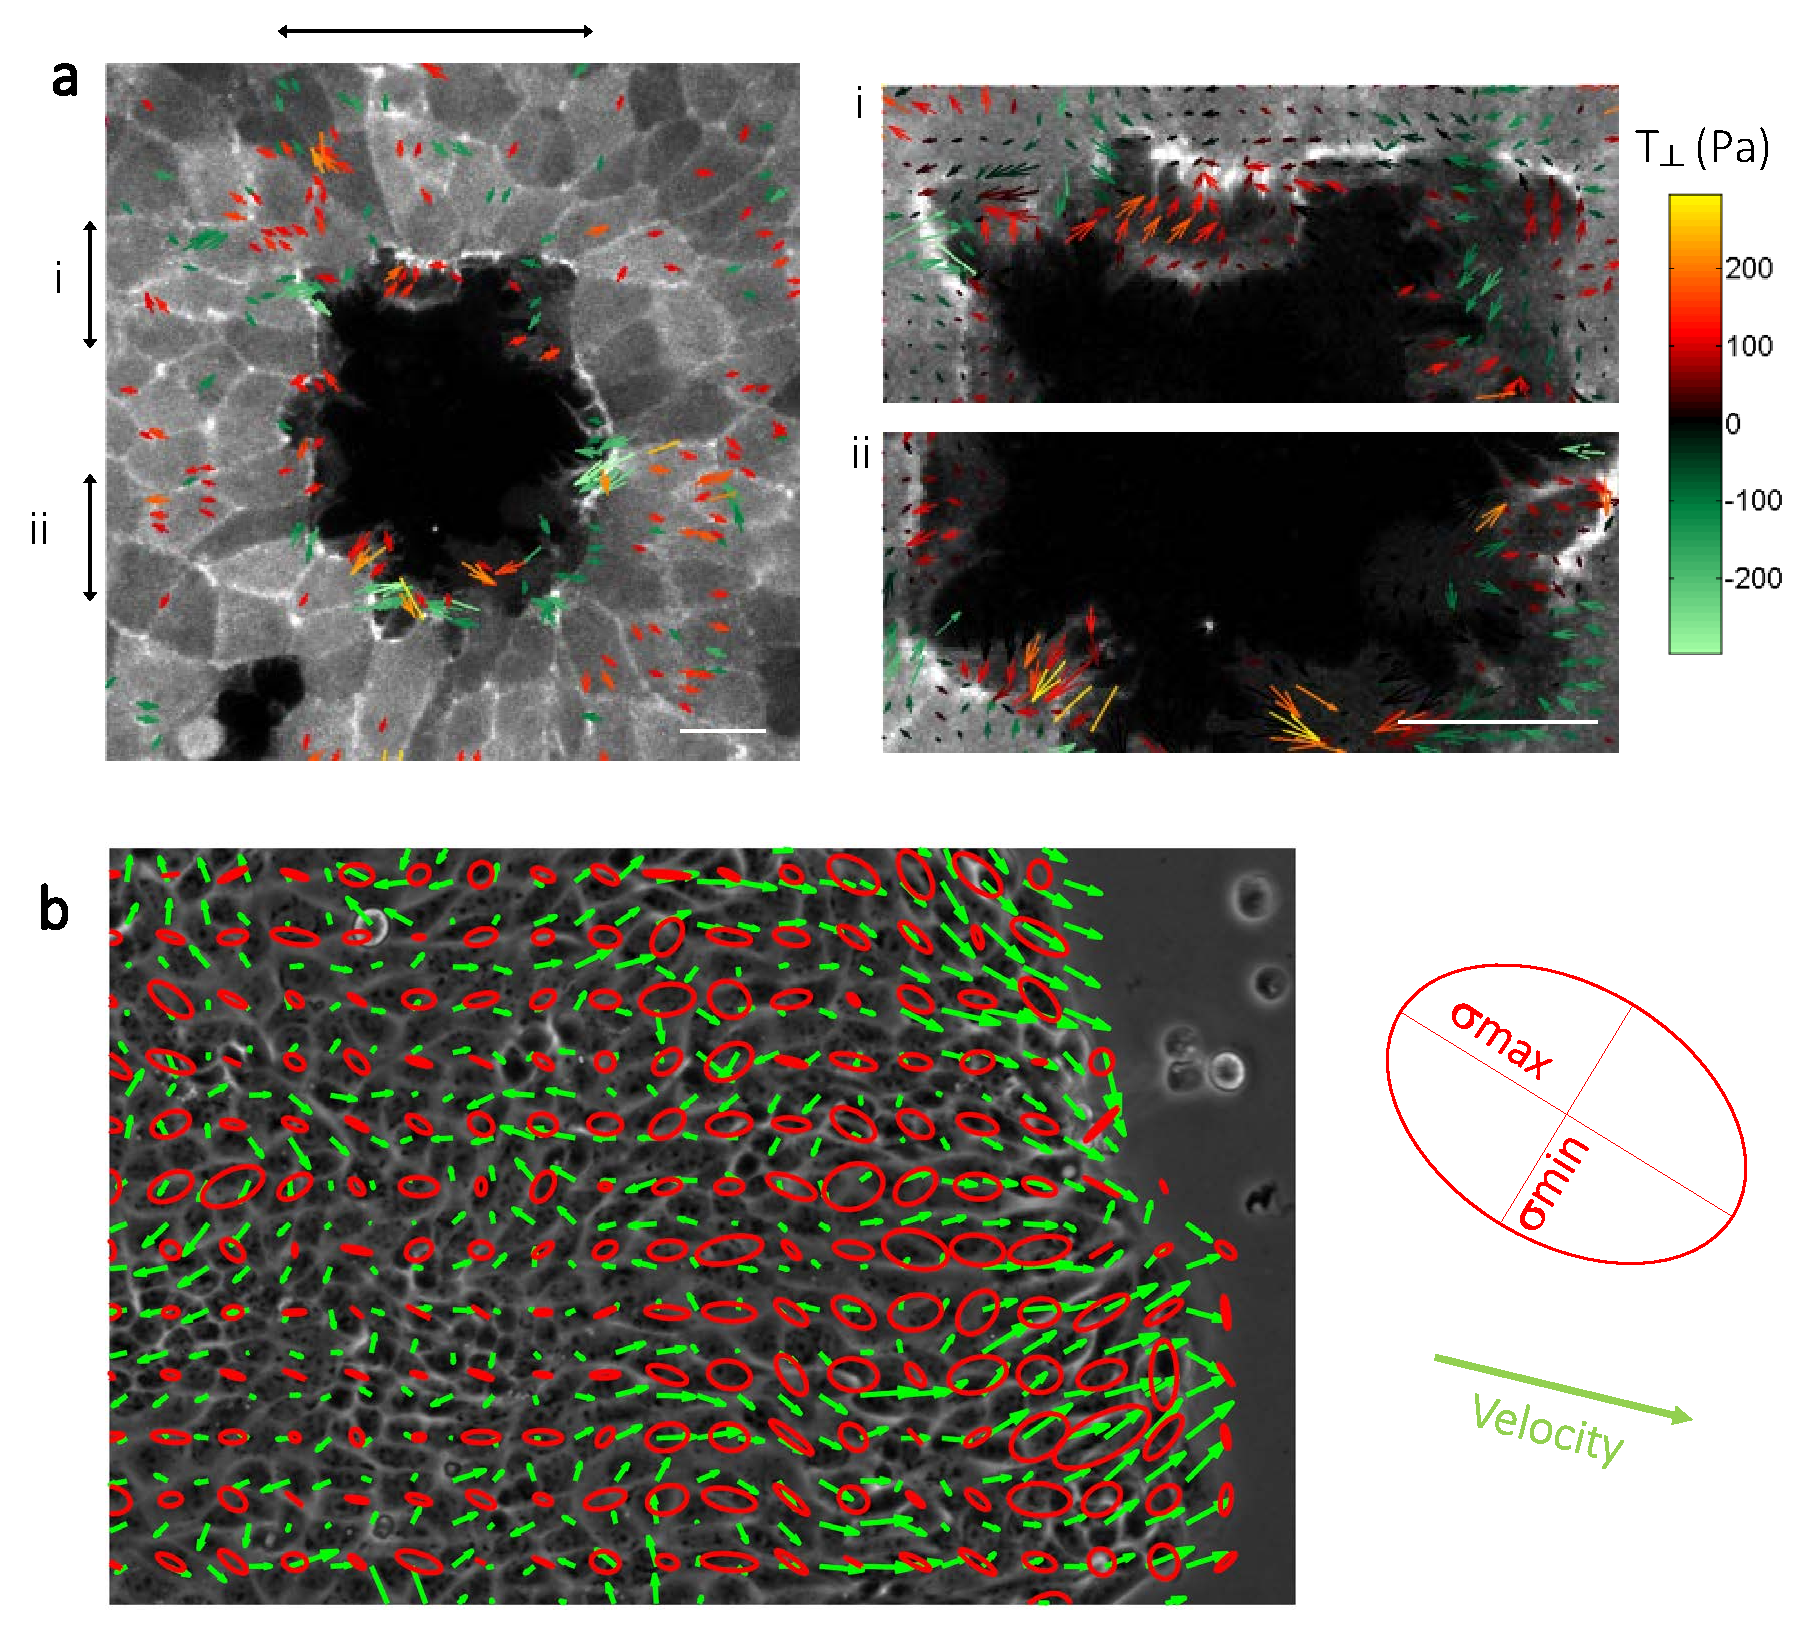
\includegraphics[width=0.8\textwidth]{intro/cell-migration.pdf}
	\caption{A figure from the paper~\cite{alert2020} illustrating cell migration during the wound healing process. 
	(a) Vector field representation of cellular traction forces in cells as they close a wound, with color intensity reflecting the radial component (positive values indicate outward-directed forces). 
	Panels labeled i and ii present magnified views of the regions marked by arrows in panel (a). 
	(b) Velocity vectors (green) and monolayer stress ellipses (red), depicting the principal stress directions and magnitudes, in a growing cell colony (phase contrast). 
	}
	\label{fig:woundhealing}
\end{figure}

In contrast, cancer cells often invade tissues as sheets, strands, or clusters, navigating a complex three-dimensional extracellular matrix (ECM) environment~\cite{friedl2009, cai2014, clark2015}. \\
While cell migration occurs extensively in three dimensions, modeling these complex processes remains a significant challenge. 
Consequently, much current scientific work focuses on two dimensional systems as a more tractable approach to understand the underlying physical principles.
Throughout this thesis, we consider cell dynamics within a bounded two-dimensional domain, denoted by $\Omega \subset \R^2$. 
Throughout this work, the total number of cells present within the domain $\Omega$ is denoted by $N_V \in \N$. \\
In two dimensions, cell monolayers serve as fundamental model systems to study cell behavior and tissue function. 
These systems, comprising a single layer of cells grown on a surface, can be mathematically and computationally modeled in either a confluent or non-confluent manner. 
A confluent cell model depicts a continuous, tightly packed layer where cells cover the entire surface without gaps, whereas a non-confluent monolayer represents a state with spaces and gaps between individual cells or cell clusters that have not yet achieved full surface coverage. \\
Recent years have seen growing interest in understanding the principles governing collective cell migration in confluent cell monolayers and epithelial tissues, which exhibit remarkable patterns and correlations in both structural arrangements and actively driven flows~\cite{wenzel2021}. 
Experimental studies on model systems have revealed phenomena such as unjamming transitions, spontaneous vortex formation, topological defects, and active turbulence. 
A key challenge is linking this macroscopic behavior to the properties of individual cells and their interactions, leading to a diverse range of modeling approaches spanning different levels of coarse-graining, from subcellular lattices and multiphase field models to vertex, Voronoi, particle, and continuum models. 
The systematic comparison of these diverse cell models is crucial for selecting appropriate methods for future studies and enabling predictive simulations of patterns and correlations in cell colonies. \\
Understanding the diffusion behavior of cells, influenced by various forces and interactions, is a key aspect of collective cell migration. This will be a central focus of this thesis. Different mathematical cell models, incorporating distinct cell dynamics, will exhibit varying diffusion behaviors. To begin this investigation, we will first introduce the simplest model: the point particle model. \\

\textbf{Point particle model} \\
We consider the point particle model on a two dimensional bounded domain $\Omega \subset \mathbb{R}^2$, where we have $N_V \in \N$ particles.
These particles have no real size.
There is also no particle interaction, as there is no possibility of collision. \\
Initially, the particles are randomly distributed in $\Omega$. \\
The particles' dynamics are governed solely by Brownian motion.
Brownian motion is a random and unpredictable motion that occurs in the real world when particles are suspended in a fluid and collide with surrounding molecules. \\
In mathematics, we model Brownian motion using stochastic differential equations (SDEs), which are equations that describe the motion of a particle over time in a random and unpredictable manner. 
SDEs are a powerful tool for modeling complex phenomena in physics, finance, and other fields, and are characterized by the presence of random terms that capture the uncertainty of the system. \\
Let 
\[\vec{x}_i(t) \in \Omega \quad 1 \leq i \leq N,\]
be the location of the particle $i$ at time $t > 0$. 
The particle movement can be modeled using the diffusion equation, which describes the random motion of particles over time
\begin{center}
	$d\vec{x}_i(t) = \sqrt{2D} \: dB_t^{(i)}, \quad 1 \leq i \leq N$,
\end{center}
where the constant $D > 0$ represents the diffusion coefficient which proportionally scales the speed of the particle movements by scaling the random fluctuations.
The term $dB_t^{(i)}$ introduces the randomness of Brownian motion, where $dB_t^{(i)}$ is a normally distributed random variable that accounts for the unpredictable changes in the position of particle $vec{x}_i$ over time. \\
We also consider the probability density function $\rho(t, \vec{x})$, which describes the probability of finding a particle at a specific position $\vec{x}$ at time $t$.
In the given context, the function $\rho$ satisfies the partial differential equation:
\begin{align}
	\dfrac{\partial \rho (t, \vec{x})}{\partial t} = D \Delta_{\vec{x}} \rho(t, \vec{x}) \label{eq:pointparticle}, 
\end{align}
where $\Delta_{\vec{x}}$ is the Laplacian operator with respect to the spatial variables. \\
Equation~\eqref{eq:pointparticle} represents the classic diffusion equation, a cornerstone of physics and mathematics.
The same diffusion constant $D>0$ is used in the SDE for particle movement and the PDE for the probability density function $\rho$. \\



% intro hp model 
\textbf{Hard sphere model} \\
Next, we consider models that add a real size to the particles and introduce particle interactions. 
With the inclusion of a real size, the particles cannot overlap, resulting in exclusion effects. 
To account for this, we introduce a new interaction dynamics that ensures the particles do not overlap. 
This new interaction dynamics leads to a more complex and realistic model that captures the behavior of particles with a real size and interactions. \\
Since particles cannot overlap, the domain $\Omega^{(i)}_{\epsilon}$, that holds the information where the centre of particle $i$ can be located, must exclude the areas where $\norm[\vec{x}_i - \vec{x}_j] \leq \epsilon$ for all $1 \leq j \leq N,$ $j \neq i$. 
This is due to the fact that particles cannot occupy the same space simultaneously. \\
The domain that holds all possible locations of the particles is then given by \[\Omega^N_{\epsilon} = \Omega^{(1)}_{\epsilon} \times \ldots \times \Omega^{(N)}_{\epsilon} .\] 
This can be visualized as a product space, where each particle's domain is combined to form a larger domain that encompasses all possible locations of the particles.
Under this circumstances, we will get a new dynamic compared to the point particle model.  \\
In the work of Bruna et al.~\cite{Bruna2012}, a hard sphere particle model is examined.
Here, the particles are spherical in shape, with a diameter $0 < \epsilon \ll 1$.
All particles in this model are distinct and can be distinguished from one another. \\
The hard sphere model is characterized by the fact that any interaction between particles may cause a change in their direction of motion, but the spherical shape of the particles remains unchanged.
Hardcore collisions are modeled as reflective boundary conditions on the collision surfaces defined by $r = \norm[\vec{x}_i - \vec{x}_j] = \epsilon$, where $1 \leq i < j \leq N$.
The external forces acting on a particle in the system are described by the force function $f: \R^2 \rightarrow \R^2$, which depends only on the location of the particle.
The function $\vec{F}$ maps the particle configuration $\vec{X} = (\vec{x}_1, \ldots, \vec{x}_N)^T$ to the vector of external forces $\vec{F}(\vec{X}) = (f(\vec{x}_1), \ldots, f(\vec{x}_N))^T$.
The dynamics of the particles are governed by the SDE
\begin{center}
	$d\vec{x}_i(t) = \sqrt{2D} \: dB_t^{(i)} + f(\vec{x}_i(t)) \: dt, \qquad 1 \leq i \leq N$.
\end{center}
In this model, the particles are initially randomly distributed in $\Omega^N_{\epsilon}$, ensuring that no overlap occurs between the particles.
The joint probability density function $P$ of the $N$ particles satisfies the high-dimensional Fokker-Planck equation
\begin{center}
	$\dfrac{\partial P}{\partial t} = \nabla_{\vec{X}} \cdot (D \nabla_{\vec{X}} P - P \vec{F})$,
\end{center}
where $\nabla_{\vec{X}}$ and $\nabla_{\vec{X}} \cdot$ denote the gradient and divergence operators with respect to the $N$-particle position vector $\vec{X}$.\\
Using the method of matched asymptotic expansions, the authors also derived the probability density function $\rho$ of finding a single particle at time $t$ and position $\vec{x}$, which satisfies the equation
\begin{align}
	\dfrac{\partial \rho (t, \vec{x})}{\partial t} = \Delta_{\vec{x}} \rho + \alpha_d (N - 1) \epsilon^d \Delta_{\vec{x}} (\rho^2) - \nabla_{\vec{x}} \cdot (f(\vec{x}) \rho).
\end{align}
When $f$ is neglected and $\epsilon \rightarrow 0$, this equation reduces to the probability density function of the point particle model, except for a rescaling factor.
Similarly, the Fokker-Planck equation is a direct extension of the diffusion equation, with an additional drift term.\\

\begin{figure}[h!]
	\centering
	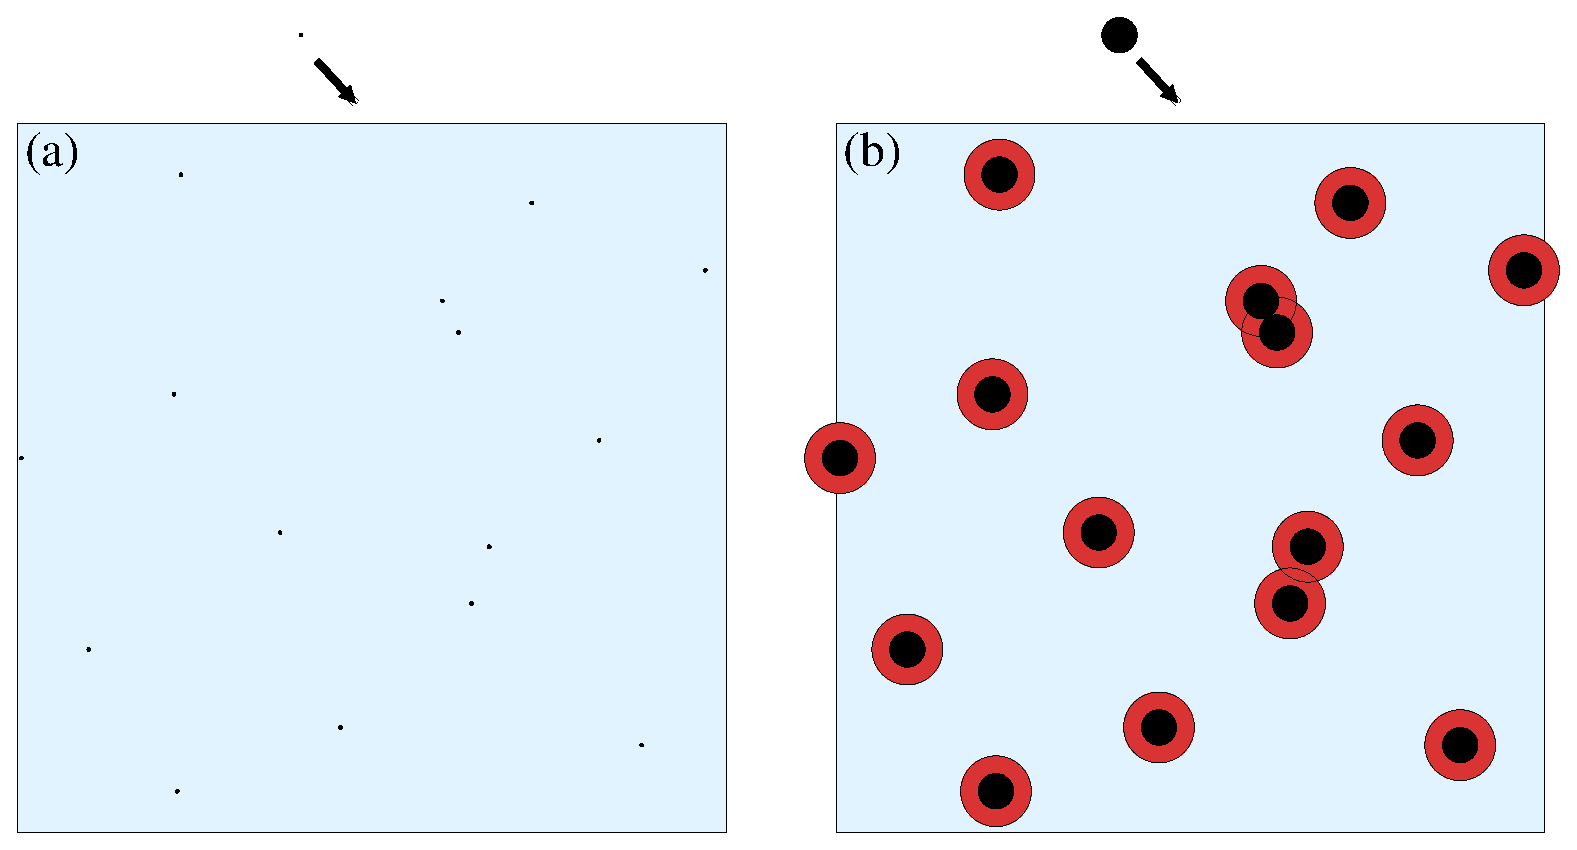
\includegraphics[width=0.8\textwidth]{intro/hardsphere.eps}
	\caption{An illustration from~\cite{Bruna2012} of the point particles on the left and the hard sphere particles on the right. We can see areas where the centre of the particles cannot be located, as they would overlap with other particles being marked red. 
	}
	\label{fig:curved_phasefield}
\end{figure}



% bachelor intro sp model 
\textbf{Soft sphere model} \\
Next, we consider an extension of the model by introducing deformable soft spherical particles. 
This new model incorporates the effect of deformation and interaction between particles through a potential energy function that depends on the distance between the particles.
The paper~\cite{Bruna2017}, written by Bruna, Chapman and Robinson, analyses the diffusion properties of such a model. \\
The equation of motion for each particle $i$ is given by
\begin{equation}
d\vec{x}_i(t) = \sqrt{2D} \: dB_t^{(i)} + f(\vec{x}_i(t))\: dt - \sum\limits_{j\neq i} \nabla_{\vec{x}_i} u (\norm[ \vec{x}_i(t) - \vec{x}_j(t)]) \: dt, \qquad 1 \leq i \leq N,
\end{equation}
where $\nabla_{\vec{x}_i}$ is the gradient with respect to $\vec{x}_i$. \\
The effect of the interaction potential is to cause particles to repel or attract each other depending on the distance between them, rather than simply overlapping. \\
For the modeling of short range interacting soft sphere particles, the authors computed the one particle probability density $\rho(t, \vec{x})$ of finding a given particle at position $\vec{x}$ at time $t$ developing according to
\begin{equation}
\dfrac{\partial \rho}{\partial t} = \nabla_{\vec{x}} \cdot (D \nabla_{\vec{x}} \rho - f(\vec{x}) \rho + \alpha_u \epsilon_u^2(N-1)\rho \nabla_{\vec{x}} \rho)
\end{equation}
where $\alpha_u$ depends on the interaction potential $u$ and $0 < \epsilon_u \ll 1$ is the interaction range of $u$.
% TODO: mention that figure 2 
\begin{figure}
	\centering
    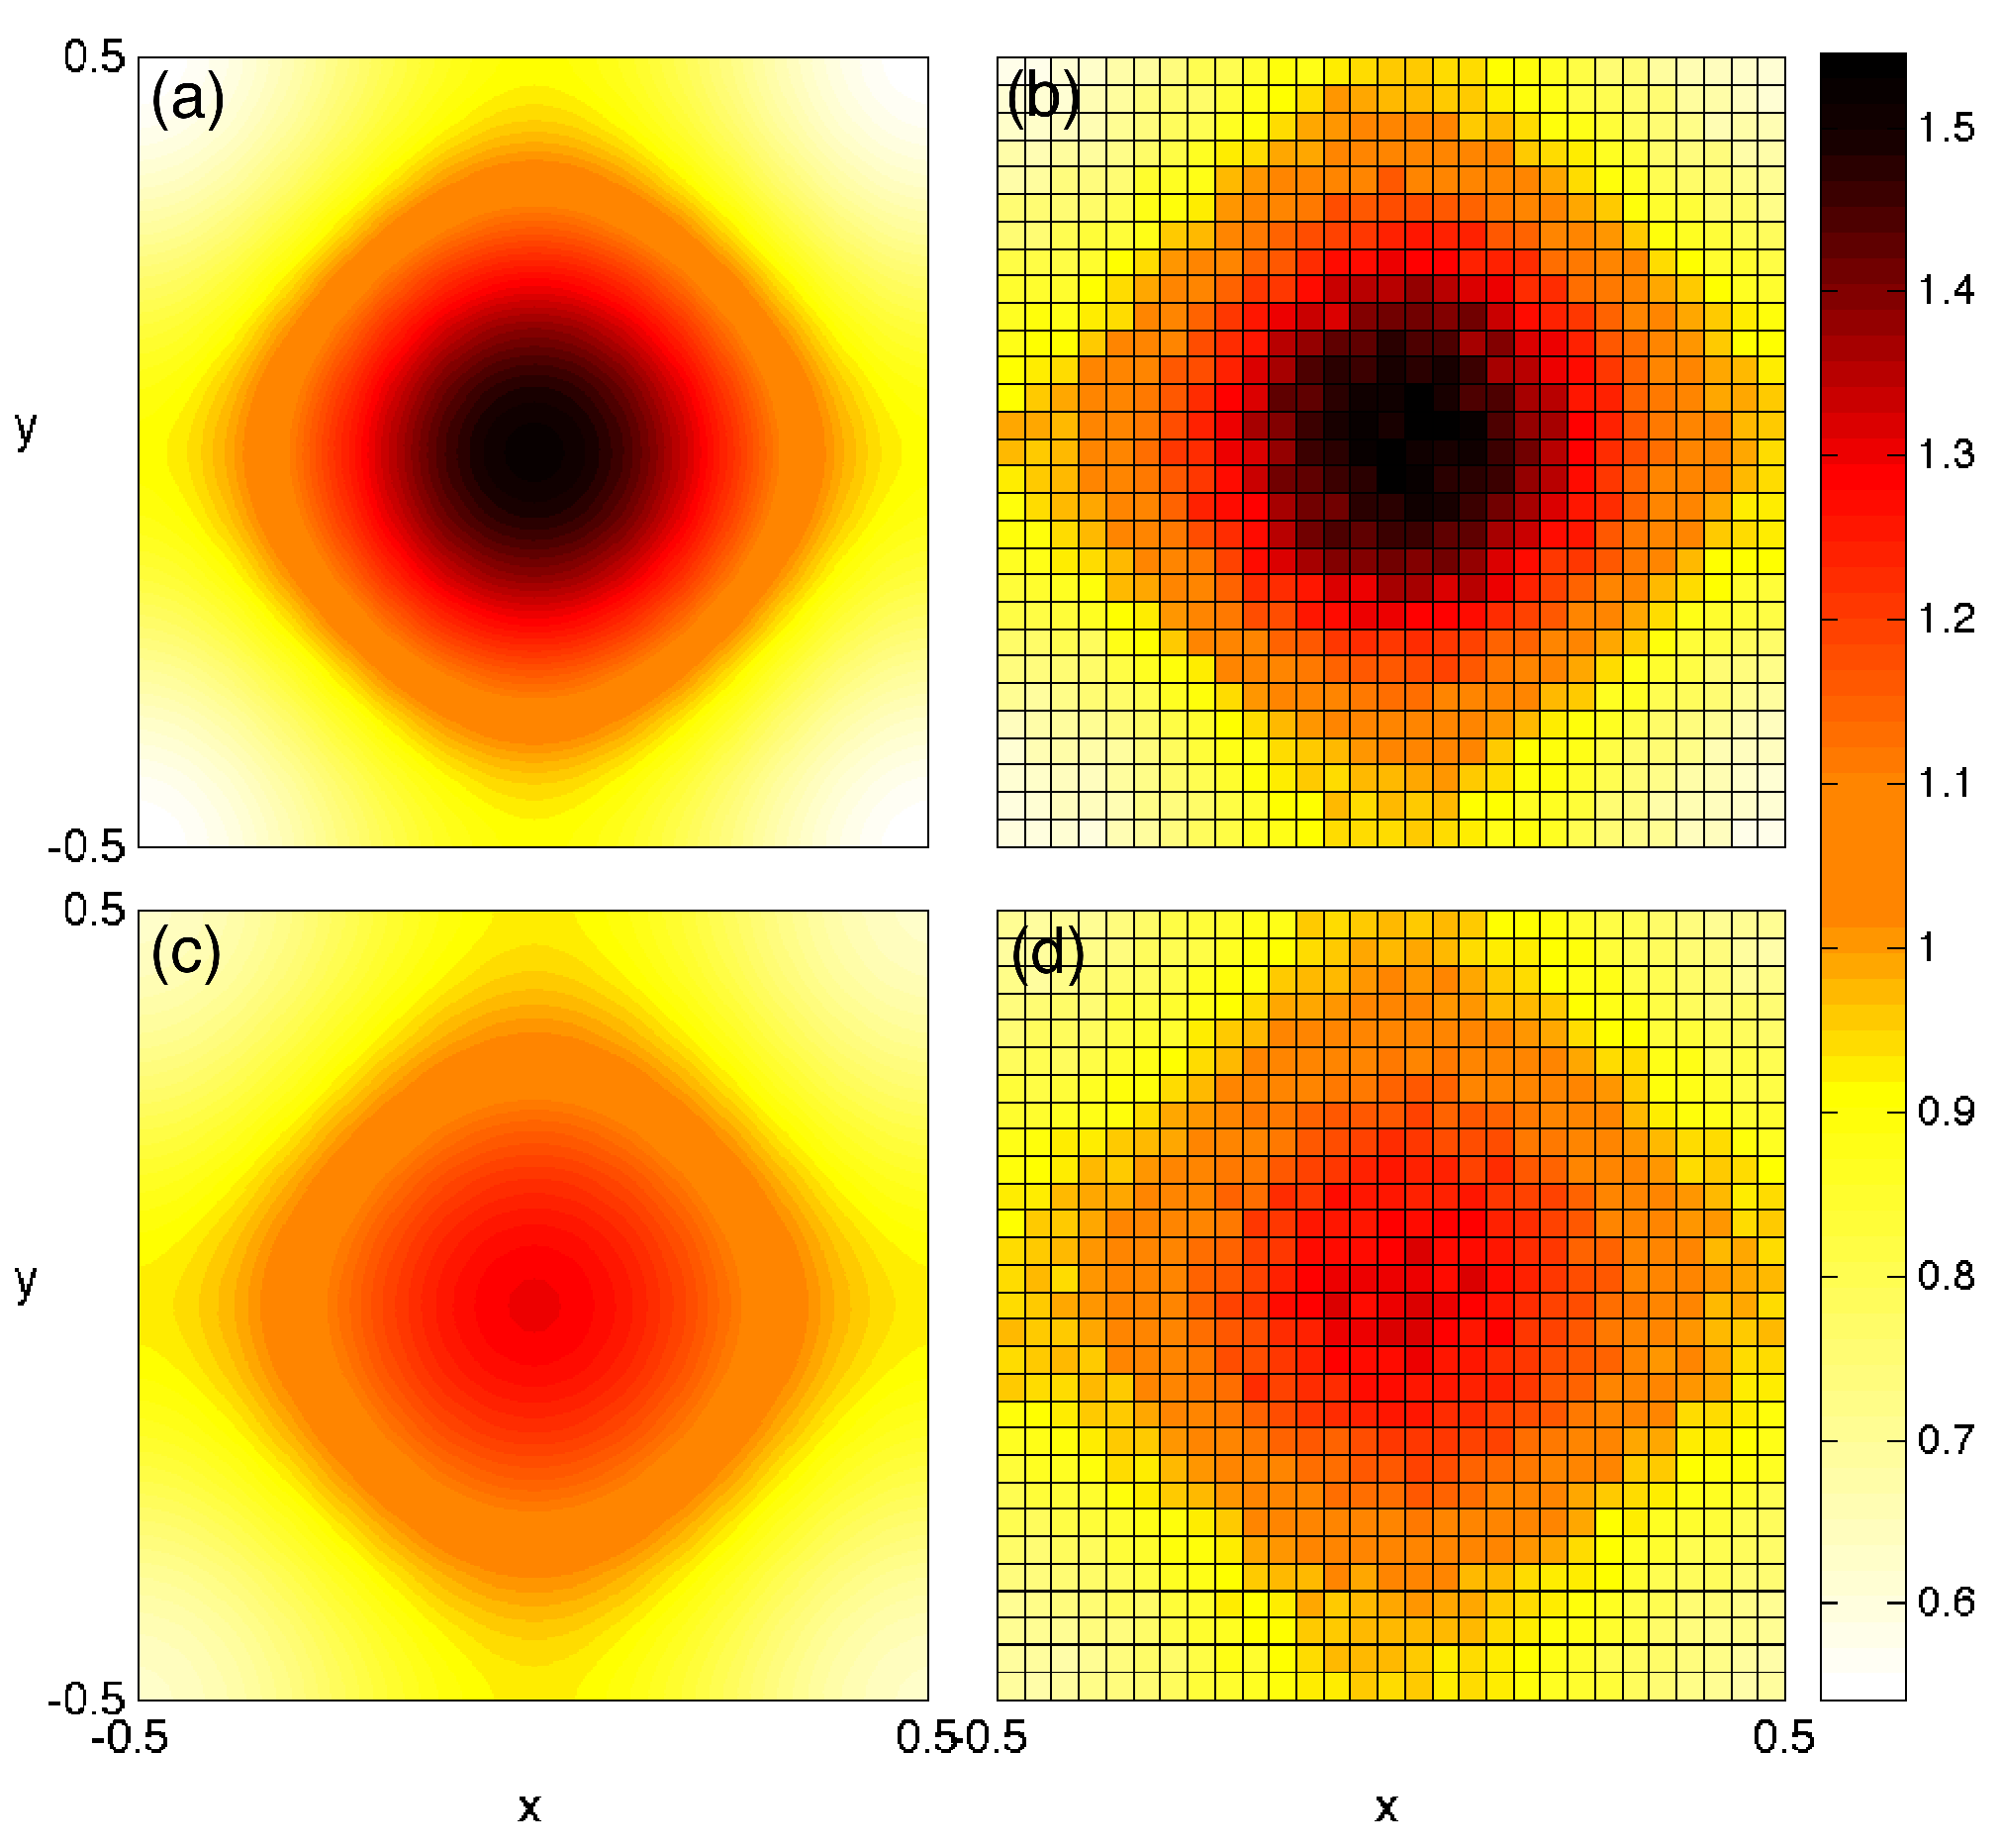
\includegraphics[width=0.8\textwidth]{intro/fig2_BC12.png}
    \caption{
    This figure contains the following four plots, all of them are shown at time \( t=0.05 \): 
    (a) shows the solution of the linear diffusion equation~\ref{eq:heat} for point particles. 
    (b) shows the histogram of a Monte Carlo simulation of the point particle model. 
    (c) shows the solution of the nonlinear diffusion equation~\ref{eq:hard-sphere-p} for finite-sized particles. 
    (d) shows the histogram of a Monte Carlo simulation of the HSCM. 
    The Monte Carlo simulations used $10^4$ simulation runs each with a time step size of $10^-5$.
    }
    \label{fig:fig2BC12}
\end{figure}
In this thesis, we aim to derive forces that can be applied to our cell model and affect the diffusion behavior of the cell system, similar to the forces studied in~\cite{Bruna2012} and~\cite{Bruna2017}. \\



% transition to phase field models 
While these models are powerful, they are limited to spherical particles and do not account for the complex shapes and deformations observed in biological cells.  \\


% phase field model
\textbf{Phase field models} \\

% intro phase field model: 
- A new cell model approach is now considered. 
- The principle of phase field models shares conceptual similarities with the soft-sphere model of Bruna, Chapman, and Robinson~\cite{BCR17} in that both incorporate cell-cell interactions through a continuous, repulsive energy term that prevents interpenetration. 
- In both frameworks, the interaction is mediated by a smooth, short-range potential (via the diffuse interface in the phase field model and via a potential 
u in the soft-sphere model), leading to a physically realistic representation of cell crowding. 
However, the phase field model differs fundamentally in its approach: it is a continuum differential equations-based model that explicitly represents cell shape and internal structure through a phase field variable $\phi_i$, allowing for complex deformations, topological changes, and geometric coupling to surface curvature. 
- In both models, cell-cell interactions are mediated through a continuous, short-range potential that prevents interpenetration while allowing for deformations, leading to a smooth transition between overlapping and non-overlapping states. 
- The soft-sphere model derives its interaction term from a potential energy function $u(\|\vec{x}_i - \vec{x}_j\|_2)$, which results in a nonlinear diffusion equation with a density-dependent diffusion coefficient. Similarly, the phase field model uses a diffuse interface representation where the interaction energy arises from a non-local term in the free energy, effectively generating a repulsive force between cells that scales with local cell density. 
- These shared mathematical structures and physical principles — namely, gradient flow dynamics, continuous interactions, and density-dependent diffusion — highlight the conceptual and formal parallels between the phase field approach and the soft-sphere model. \\
- While the phase field model shares core principles with the soft-sphere model—such as continuous interactions and density-dependent diffusion—it differs significantly from both the soft-sphere and hard-sphere models in its representation and physical implementation. 
Unlike the soft-sphere model, which treats cells as point particles with a smooth interaction potential, the phase field model explicitly represents cells as extended, diffuse regions with a continuous internal structure defined by the phase field variable $\phi_i$. \\

This allows for natural handling of complex cell shapes, topological changes (such as cell division or fusion), and the coupling of cell mechanics to geometric curvature through extrinsic curvature terms in the free energy. 
- the phase field model resolves overlaps through gradual, continuous deformation of cell interfaces, avoiding discontinuities in dynamics. 
- Both frameworks are based on a variational principle, where cell dynamics are governed by a gradient flow of a free energy functional that incorporates shape preservation, cell-cell interactions, and the physical constraints of the system. 
- contrasts to the sphere models are: 
- the hard-sphere model enforces rigid, non-deformable boundaries via reflective boundary conditions at a fixed distance, resulting in abrupt, instantaneous collisions without shape deformation.  The phase field model, by contrast, resolves overlaps through gradual, continuous deformation of cell interfaces, avoiding the discontinuities inherent in hard-sphere dynamics. \\

Phase field variables represent cells as smooth functions $\phi_i(\vec{x}, t) \in [-1, 1]$, with $\phi_i > 0$ in the cell interior and $\phi_i <0$ in the exterior. 
The cell wall is denoted by values of $\phi_i = 0$. \\
\begin{figure}[h!]
	\centering
	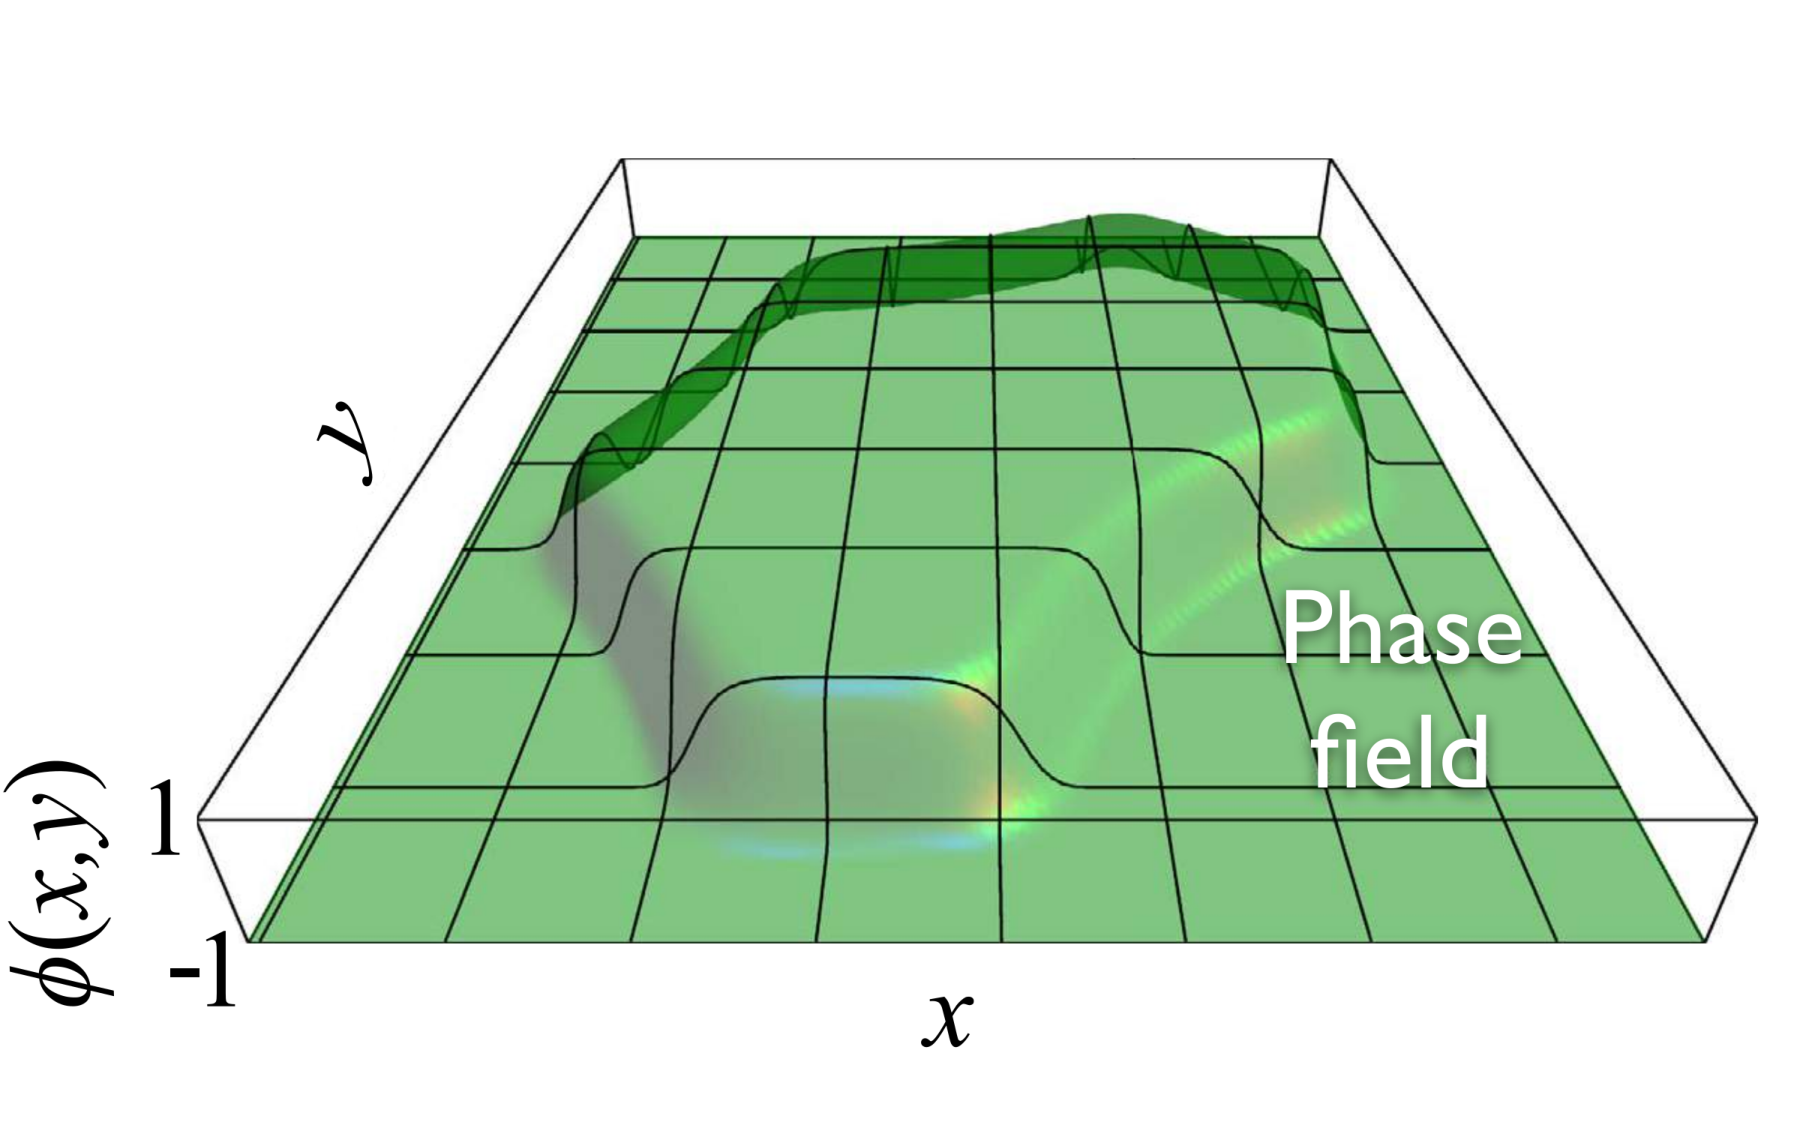
\includegraphics[width=0.8\textwidth]{intro/phasefield.pdf}
	\caption{A snapshot from the paper~\cite{alert2020} illustrating a phase field variable. 
	The cell's inside has value $\phi = 1$ and the outside $\phi = -1$. 
	}
	\label{fig:phasefield}
\end{figure}
	
The dynamics of $\phi_i$ are governed by a gradient flow of a free energy functional:
\begin{align*}
	\frac{\partial \phi_i}{\partial t} + v_0 (\vec{v}_i \cdot \nabla_{\vec{x}} \phi_i) = \Delta_{\vec{x}} \frac{\delta F}{\delta \phi_i}, \qquad 1 \leq i \leq N 
\end{align*}
where $\vec{v}_i$ is a vector field used to incorporate activity, with a self propulsion strength $v_0$, $F$ is a free energy, and $\dfrac{\delta F}{\delta \phi_i}$ denotes the first variation.\\
The free energy $F$ arises from a sum of different energies, 
\begin{align*}
	F = F_{CH} + F_{INT} + F_{M}. \\
\end{align*}
The first energy is a Cahn-Hilliard energy and could look like in~\cite{wenzel2021}
\begin{align*} 
	F_{CH} = \sum\limits_{i=1}^N \int_{\Omega} \dfrac{1}{Ca} \left( \dfrac{\epsilon}{2} \norm[\nabla_{\vec{x}} \phi_i]^2 + \dfrac{1}{\epsilon} W(\phi_i) \right) d\vec{x},
\end{align*}
$\epsilon$ is a small parameter related to the interface thickness, and $Ca$ is a capillary number that scales the relative importance of surface tension.
The term $\norm[\nabla_{\vec{x}} \phi_i]^2$ penalises a long cell wall, as $\nabla_{\vec{x}} \phi_i \neq 0$ only at the cell wall.
$W(\phi_i) = \dfrac{1}{4} (\phi_i^2 - 1)^2$ is a double-well potential. 
This energy ensures that each $\phi_i$ maintains a stable interface of $[-1,1]$.  \\ 
The second energy term $F_{INT}$ models cell-cell interactions and could be defined as in~\cite{wenzel2021}
\begin{align*}
	F_{INT} = \sum\limits_{i=1}^N \frac{1}{Ca} \int_{\Omega} B(\phi_i) \sum\limits_{j \neq i} w(d_j) \: d\vec{x},
\end{align*}
where 
\[B(\phi_i) = \dfrac{3}{4\sqrt{2}\epsilon} (\phi_i^2 - 1)^2\]
is an approximation of the delta function of the cell boundary that is non-zero only at the cell wall.
The sum in the integral accounts for the interaction with all other cells $j \neq i$ through a short-range potential $w(d_j)$, where $d_j$ is the signed distance function to the cell boundary of cell $j$.  

The third energy term $F_M$ differs for different models and incorporates additional mechanical properties of the cells, such as area conservation or bending energy.
% phase field comparison paper:

- In \cite{wenzel2021}, the authors focussed on the influence of microscopic details to incorporate active forces on emerging phenomena.
The models are based on cell deformations and cell-cell interactions and we investigate 
- We compare four different approaches, one in which the activity is determined by a random orientation, one where the activity is related to the deformation of
the cells, and two models with subcellular details to resolve the mechanochemical interactions underlying cell
migration.
- The models are compared with respect to generic features, such as coordination number distribution,
cell shape variability, emerging nematic properties, as well as vorticity correlations and flow patterns in large
confluent monolayers and confinements. 
- The random model determines the direction of motion on the single cell level by a stochastic process
- elongation model aligns the direction of motion with the long axis of the cell
- polar and a nematic model, which use subcellular details to determine strength and direction of motion on a single cell level.

- The goal of this paper is a systematic comparison of these approaches and their linkage with statistical observables of experiments to provide a route towards predictive simulations of patterns and correlations in cell colonies. After introducing the multiphase field models, discussing microscopic differences, and briefly describing the numerical approach enabling large-scale simulations, we address coordination number distribution, analyze statistics on shape variability of the cells and the ratio of multicellular rosettes, velocity distributions of emerging topological defects, their stress fields, as well as defect density and creation rates
- All results are compared with experimental data for a large variety of cell cultures. The appearing qualitative differences of the models show the importance of microscopic details.

\begin{table*}[h!]
\centering
\begin{tabular}{>{\scriptsize}l >{\small}c  >{\small}c  >{\small}c  >{\small}c} % l = left aligned, c = centered, r = right aligned
\hline
characteristic & Random & Elongation & Polar & Nematic \\ 
\midrule
Coordination number distribution & ($\checkmark$) & ($\checkmark$) & ($\checkmark$) & ($\checkmark$) \\[0.5em]
Shape variability & ($\checkmark$) & $\checkmark$ & $\checkmark$ & ($\checkmark$) \\[0.5em]
Rosette ratio & \multicolumn{4}{>{\small}c}{Differences between models} \\[0.5em]
Velocity distribution of topological defects & \multicolumn{4}{>{\small}c}{Differences between models} \\[0.5em]
Correlation between direction of motion and orientation of defect & $\boldsymbol{\times}$ & $\checkmark$ & $\checkmark$ & ($\checkmark$) \\[0.5em]
Elastic property of + 12 defect & $\boldsymbol{\times}$ & Extensile & Contractile & Contractile \\[0.5em]
Active turbulence & ($\checkmark$) & ($\checkmark$) & ($\checkmark$) & ($\checkmark$) \\[0.5em]
Vorticity-vorticity correlation & \multicolumn{4}{>{\small}c}{Similar for all models} \\[0.5em]
Dependency of defect density on activity & Linear & Linear & Linear & Constant \\[0.5em]
Rotational motion in circular confinement & $\boldsymbol{\times}$ & ($\checkmark$) & $\boldsymbol{\times}$ & $\boldsymbol{\times}$ \\[0.5em]

\bottomrule
\end{tabular}
\caption{Comparison of the four different phase field models from~\cite{wenzel2021} with respect to various characteristics observed in experiments. 
A check mark $\checkmark$ indicates observed agreement, $\boldsymbol{\times}$ indicates disagreement and ($\checkmark$) indicates only qualitative agreement with universal feature. 
If experimental data are not available or insufficient for a comparison, only similarities or differences of the models are noted.}
\end{table*}
% phase fields on curved domains 
- Another work that uses phase field models to describe cell dynamics is~\cite{Happel2023} by Axel Voigt and Lea Happel.
- this work focuses on the impact of curved domains on the collective behavior of cells, defining the phase fields on tori. 
- it focuses on emergent collective behaviors such as coordinated rotation on curved surfaces, driven by curvature alignment and self-propulsion. 
- while the soft-sphere model typically assumes spherical symmetry and isotropic interactions, the phase field model can incorporate anisotropic effects—such as alignment with principal curvature directions—through geometric coupling terms, enabling the simulation of complex collective behaviors like coordinated rotation on curved surfaces. 
These differences make the phase field model more biologically realistic for epithelial tissues, but also more computationally demanding than the simpler point-particle approaches. 
- The phase field model developed by Happel and Voigt \cite{HV23} demonstrates that extrinsic curvature coupling is essential for explaining the alignment of cell elongation with principal curvature directions and the emergence of coordinated rotational motion in epithelial layers on curved surfaces. Their simulations reproduce key experimental observations—such as spontaneous rotation on cylinders and curvature-dependent shape changes on tori—by combining a diffuse interface representation with a free energy that includes both intrinsic and extrinsic geometric terms. This work underscores the importance of geometric effects in tissue morphogenesis and provides a framework for studying how curvature influences collective cell behavior beyond flat, two-dimensional environments.

\begin{figure}[h!]
	\centering
	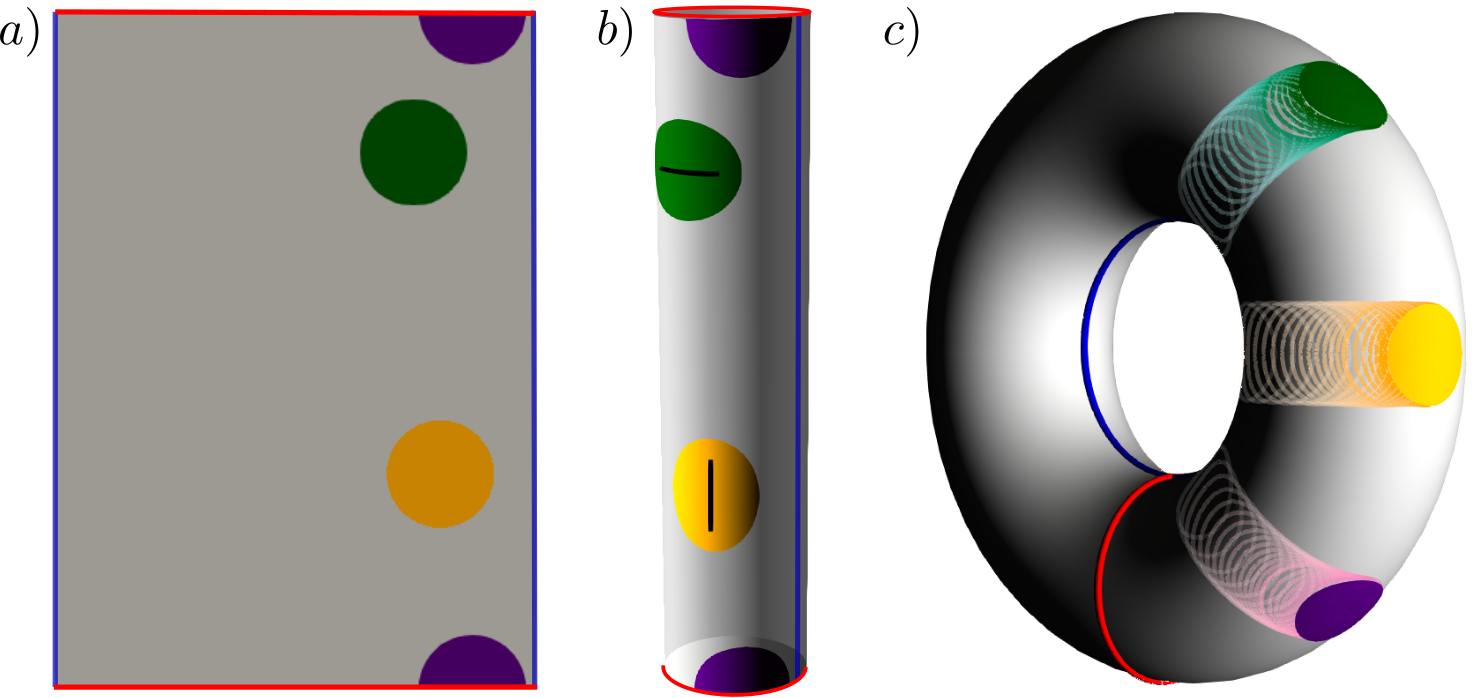
\includegraphics[width=0.8\textwidth]{intro/curved_phasefield.png}
	\caption{A figure from the paper~\cite{Happel2023} showing a phase field variable $\phi$ on a curved domain, specifically a torus. 
	In (a) and (b), the surface of the torus from (c) is shown as a parametrization on a rectangle, where the blue edges are identified (glued together) to form the toroidal direction, and the red edges are similarly identified to form the poloidal direction. 
	Red and blue lines represent periodic boundary conditions, which are enforced by gluing the corresponding edges in (b) and (c).
	The color coding corresponds to the extrinsic curvature parameter $E_c$ (see Eq.~(3)): $E_c = 0$ (purple) results in a geodesic circle on both geometries; $E_c > 0$ (green) favors alignment with the direction of maximum absolute curvature; $E_c < 0$ (yellow) favors alignment with the direction of minimal absolute curvature. 
	Cell elongation is highlighted for visibility. 
	On toroidal surfaces, cell shape depends on position due to varying curvature. 
	(c) shows the trajectories, final positions, and shapes of cells over time. 
	The influence of extrinsic curvature is not apparent in the final configuration, as all shapes were obtained by solving Eq.~(1) with $v_0 = 0$. 
	}
	\label{fig:curved_phasefield}
\end{figure}



% vertex based model 
\textbf{Vertex models} \\

% bridge paper:
With precedents in the physics of foams, network models describe epithelial tissues as networks of polygonal cells. Thus, albeit in less detail than lattice and phase-field models, these models still describe subcellular features of cell shape. They encompass two subtypes of models: vertex and Voronoi models.

- In vertex models, the degrees of freedom are the vertices of the polygons.
- Alternatively, the network can be described by the cell centers, and this reduces the number of degrees of freedom. These descriptions are known as Voronoi models because, given the positions of the cell centers, the cell-cell boundaries are delineated by the Voronoi tessellation
- The difference in the number of degrees of freedom has important consequences for the mechanical properties of the network, which may thus differ between vertex and Voronoi models 
- In Voronoi models, the network is dynamic, evolving with each recomputation of the tessellation
- In vertex models, by contrast, network rearrangements entail the appearance and disappearance of vertices, which requires implementing specific rules


% jamming 
- the paper~\cite{Boromand2018} by Boromand, Merkel and Manning, studies the jamming transition in a system of deformable cells with a vertex model. 
- whats interesting for us is its the non-confluent cell model 
- the particle model is called deformable particle (DP) model
- it can be used to model cells, foams, emulsions, and other soft particulate materials
- The DP model combines the ability to model individual soft particles with the shape-energy function of the vertex model,
- there is a shape-energy function that is minimized for area and perimeter and repulsive interparticle forces. 
- we have:
* p perimeter 
* a area 
* bond vector $\vec{l}_{mi}$ connects vertices $i$ and $i+1$ of cell $m$ that are written as $\vec{v}_{m,i}$ and $\vec{v}_{m,i+1}$, respectively.
- shape energy function:
\begin{align*}
	U &= U_{contract} + U_{compress} + U_{line tension} + U_{bending} + U_{interaction} ,
\end{align*}
\begin{align*}
	U_{contract} &= \frac{k_l N_v}{2} \sum\limits_{m=1}^{N} \sum\limits_{i=1}^{N_v} (l_{m,i}-l_0)^2,
\end{align*}
where $N_v$ number of vertices per cell, $k_l$ is spring constant, $l_0$ equilibrium length of the edges 
\begin{align*}
	U_{compress} &= \frac{k_a}{2} \sum\limits_{m=1}^{N} (a_m - a_0)^2, 
\end{align*}
where $k_a$ is compressibility constant, $a_0$ equilibrium area of the cell
\begin{align*}
	U_{line tension} &= \gamma \sum\limits_{m=1}^{N} \sum\limits_{i=1}^{N_v} l_{m,i} ,
\end{align*}
where $\gamma$ is the line tension coefficient, 
\begin{align*}
	U_{bending} &= \frac{k_b}{2 N_v} \sum\limits_{m=1}^{N} \sum\limits_{i=1}^{N_v} \left( \frac{2( \hat{l}_{m,i} - \hat{l}_{m,i+1})}{l_{m,i} - l_{m,i+1}}  \right)^2 ,
\end{align*}
where the last sum is a cyclic summation, $k_b$ is the bending rigidity constant, $\hat{l}_{m,i} = \frac{\vec{l}_{m,i}}{\norm[\vec{l}_{m,i}]} $ is the unit vector of $\vec{l}_{m,i}$


There are two different methods to model the repulsive interaction between two deformable polygons called rough surface (RS) and smooth surface (SS) method.
- In the RS method, each vertex of a polygon is treated as the center of a disk with diameter $\delta = l_0 = 1$. 
- Repulsive interactions are computed as linear spring forces between overlapping disks on contacting polygons. 
- This method effectively models a "rough" surface with discrete, localized repulsion at vertices.
\begin{align*}
	U_{RS interaction} &=  \sum\limits_{m=1}^{N} \sum\limits_{n>m}^{N} \sum\limits_{j=1}^{N_v} \sum\limits_{k=1}^{N_v} \frac{k_r}{2} (\delta - |\vec{v}_{m,j} - \vec{v}_{n,k} |)^2 \times \Theta(\delta - |\vec{v}_{m,j} - \vec{v}_{n,k}) ,
\end{align*}
where $k_r$ is the repulsive constant, $\delta$ is the diameter of the disks or width of the circulo-lines (see Fig.~\ref{fig:vertex}), and $\Theta$ is the Heaviside step function, that is either $1$ for a positive argument or $0$ otherwise. \\

- In contrast, the SS method models polygon edges as circulo-lines (i.e., line segments with finite width $\delta$). 
- The repulsive interaction is computed based on the minimum distance $d_{\min}$ between two edge segments $l_{m,j}$ and $l_{n,k}$, replacing the vertex-to-vertex distance in the RS method. 
The interaction energy becomes:
$
U_{SS interaction} = \sum_{m=1}^N \sum_{n \neq m} \sum_{j=1}^{N_v} \sum_{k=1}^{N_v} \frac{1}{2} k_r \left( \delta - d_{\min} \right)^2 \Theta\left( \delta - d_{\min} \right),
$
where $d_{\min}$ is the shortest distance between the two line segments. 
This method provides a smoother, more continuous repulsion, better approximating the behavior of soft, continuous interfaces.

Despite the different interaction mechanisms, both methods yield similar structural and mechanical properties at jamming onset. 
This indicates that the overall jamming behavior is robust to the specific choice of interaction model.
Figure~\ref{fig:vertex} illustrates the two interaction methods.

\begin{figure}[h!]
	\centering
	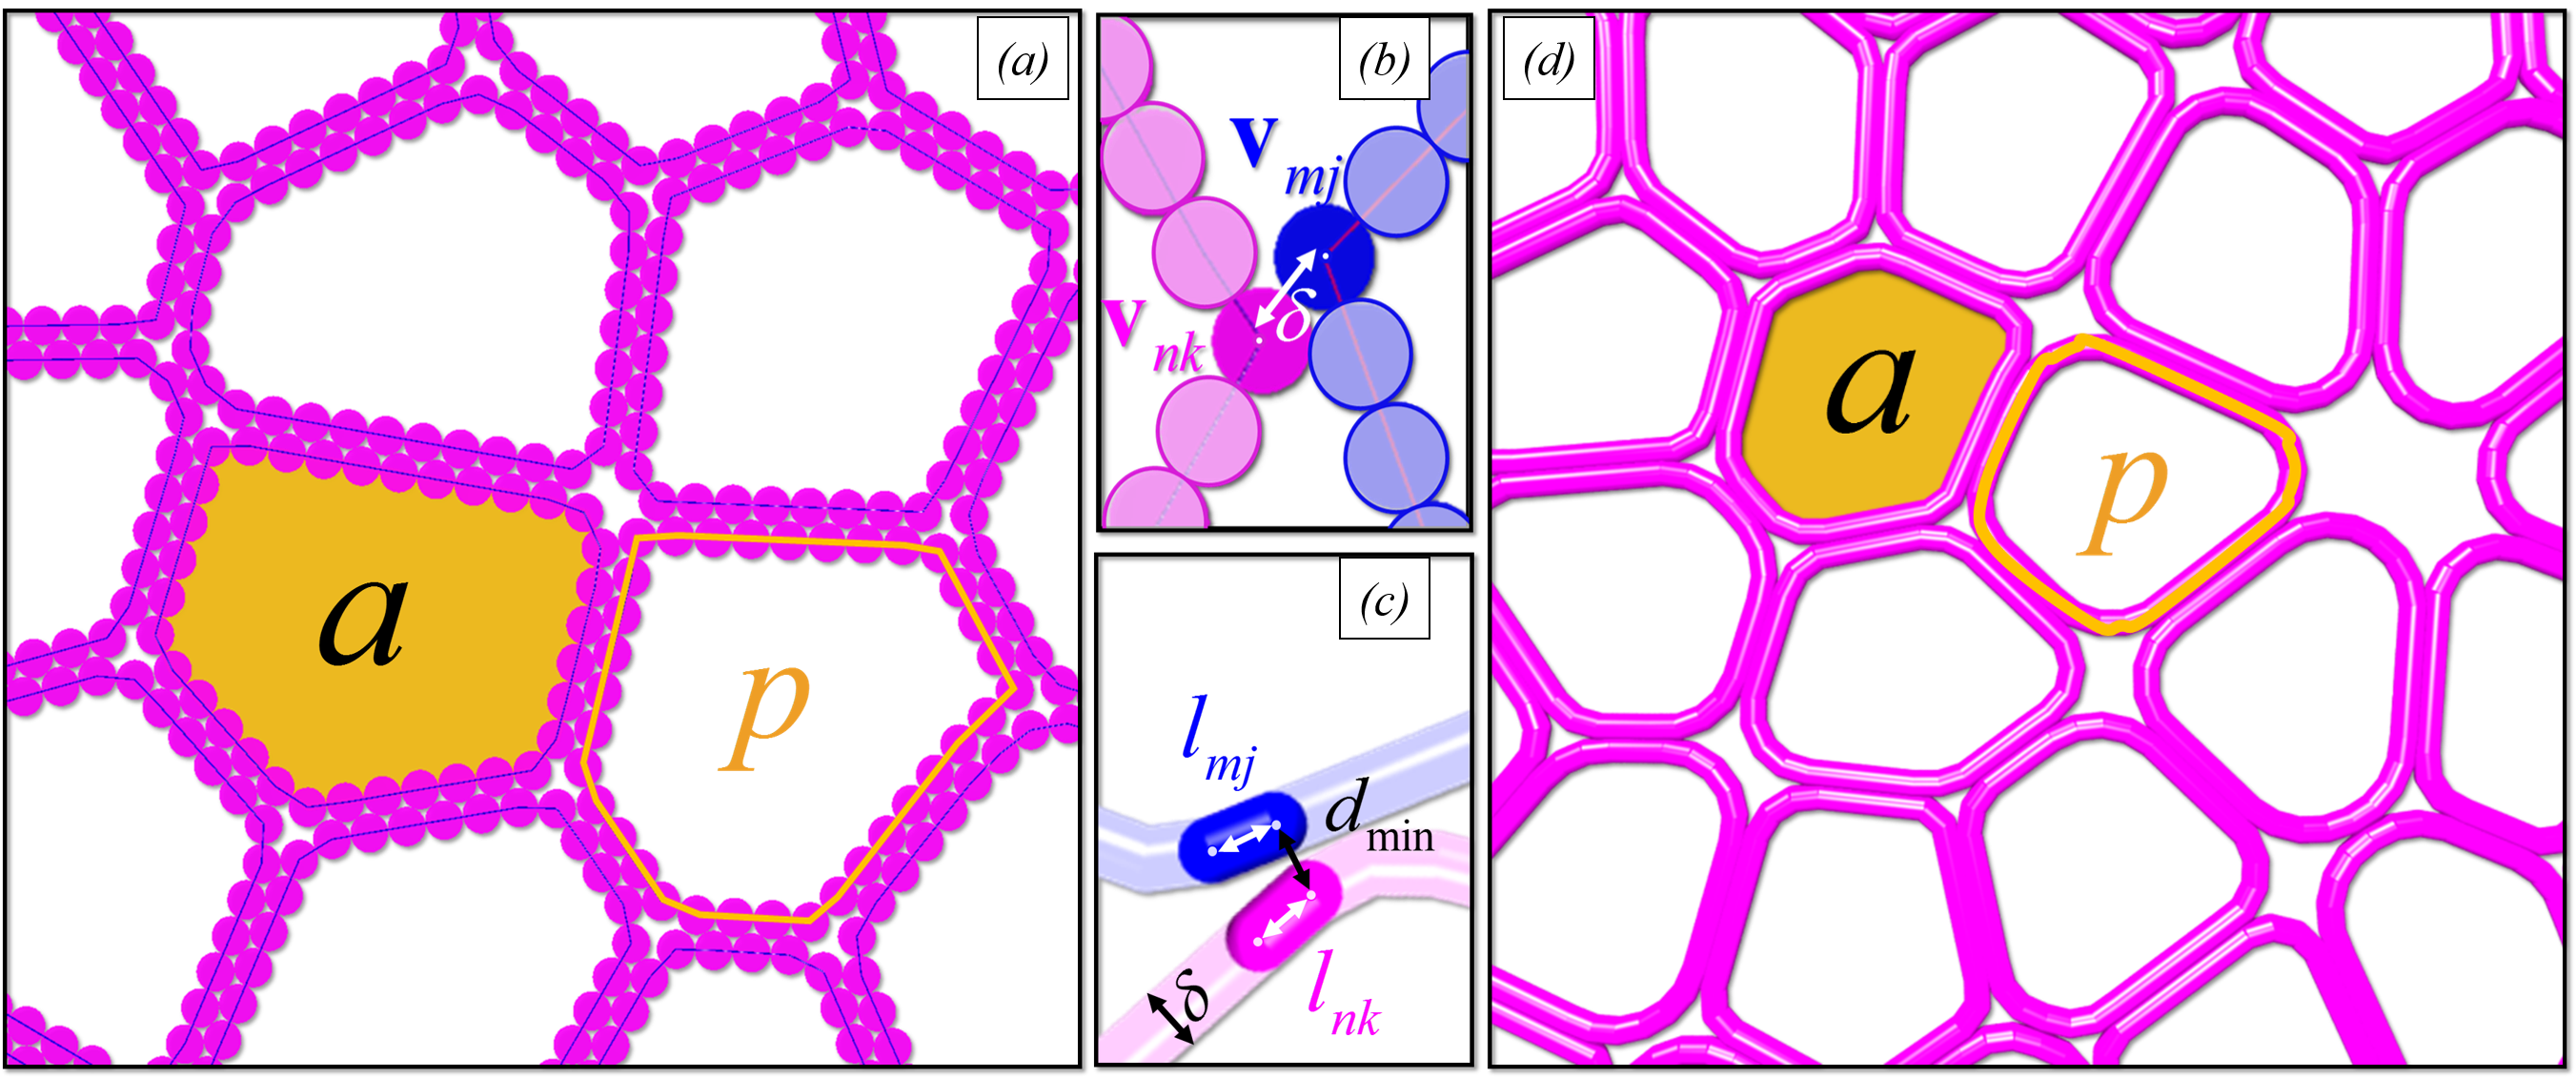
\includegraphics[width=0.8\textwidth]{intro/jamming.png}
	\caption{A snapshot from the paper~\cite{Boromand2018} illustrating a configuration of vertex-based deformable cells. 
	Schematic of deformable polygons with $N_v = 34$ vertices (where the position of the $j$-th vertex in the $m$-th polygon is denoted by $\vec{v}_{m,j}$), area $a_m$, and perimeter $p_m$. 
	The edge $l_{m,j} = p_m / N_v$ represents the line segment connecting vertices $j$ and $j+1$ in polygon $m$. 
	Two methods are used to model the edges of deformable polygons: (a) and (b) show the RS method, where disks of diameter $\delta$ are centered at the polygon vertices; (c) and (d) show the SS method, where polygon edges are modeled as circulo-lines of width $\delta$. 
	The quantity $d_{\text{min}}$ denotes the minimum distance between the line segments $l_{m,j}$ and $l_{n,k}$.
	}
	\label{fig:vertex}
\end{figure}

% fletcher 

% bachelor thesis 
A simpler approach for modeling diverse shapes in cell models is to use a vertex-based model, as used in~\cite{Fletcher14}. 
Vertex models are a valuable tool in computational biology and biophysics for studying the biomechanics and behavior of cells and tissues. \\
In a vertex model of a cell, the cell's outline or boundary is approximated as a polygon, with the vertices of this polygon representing discrete points along the cell's boundary. 
Movements or transformations of the cell are given by forces that are applied on each vertex individually. \\
The cell dynamic in a vertex model is given by the equation
\begin{align}
	\eta \dfrac{d \vec{x}_i}{dt} = F_i, \qquad 1 \leq i \leq N \label{eq:vertexmodel}, 
\end{align}
where $\eta$ is a scaling factor and $F_i$ is the total force acting on $\vec{x}_i$. \\
Like in the phase field model, $F_i$ is a sum of different forces that define the cell behavior, such as the cell flexibility or the interaction with other cells. \\
Our new cell model shall be able to represent a wide range of shapes, similar to the phase field model in~\cite{Happel2023} and the vertex model in~\cite{Fletcher14}. \\
- we have worked on the same 4 forces as in this thesis, but in the master thesis, there were many adaptations made 
- bug fixes, redefining forces with neighboring vertices, stability 
- parameter studies to find force scalings that work
- paralellisation of the code to be able to run the monte carlo sims  


%%% TODO: describe RS and SS method

% transition to our model:
\textbf{Discrete form model} \\ 
%%% TODO: explain what was done in bachelor thesis 
The DF model shares several key features with the referenced cell models. 
All frameworks after the point particles account for excluded-volume effects, which prevent cell overlap and lead to enhanced diffusion and non-trivial collective behavior. 
The dynamics in each model are governed by gradient flows of energy functionals, ensuring that the system evolves toward lower-energy configurations. 
Furthermore, stochastic motion—modeled as Brownian motion—is included in all approaches to capture thermal fluctuations. 
These shared principles provide a strong foundation for comparing our model to established frameworks.
Like the vertex model of Fletcher et al.~\cite{Fletcher14}, our cells are represented as polygons with discrete vertices, and their dynamics are governed by forces derived from energy gradients. 
However, unlike the standard vertex model, our framework explicitly incorporates a **hardness parameter $h \in [0,1]$** that allows for a continuous transition from rigid hard-sphere behavior ($h=1$) to fully deformable cell dynamics ($h=0$).
In this thesis, we derive and study a non-confluent DF model that systematically investigates how cellular deformability—controlled by the hardness parameter $h$—influences the overall diffusivity of the cell system. 
By connecting our model to the established frameworks of Bruna and Chapman~\cite{Bruna2012, Bruna2017} and Happel and Voigt~\cite{Happel2023}, we provide a unified perspective on cell dynamics that spans from rigid to deformable regimes.

%%% TODO: work in missing papers 
- we define similar energies as in~\cite{Fletcher14}, but we mostly consider simulations with only $N_V=6$ vertices per cell.  

%%% TODO: tell what happens in the following chapters 


\section{Cell model} 
* introduce the Discrete cell form (DCF) \\
- can i just reference my bachelor thesis or how should i do that? 

\subsection{Discrete cell form}
* the discrete cell form consists of a list that holds all wall points in consecutive order 

\subsection{Cell dynamics} 
* area force \\
* edge force \\
* interior angle force \\ 
* overlap force \\

\subsection{Numerical solver}
* DifferentialEquations.jl solver 
* solve(prob_cell1, EM(), dt=timeStepSize)
* -> Euler Maruyama method with fixed time step size  					
\section{DF model dynamics} \label{dynamics}
% TODOs:
% * explain what the k does to the forces (k=1 -> discrepance between current and desired state does not influence scaling of force, k=2 -> it does influence it linearly)
% * explain that we use k=1 only for deforming overlap and k=2 for shape preserving forces 
% * explain that each figure representing a force has every parameter chosen to be equivalent to the big monte carlo simulations in the next chapter: cell size, desired states (perfect 6eck with distance 0.005 from each vertex to the cell centre), force scalings, time step size  
% * explain that we tried to use unfavourable initital states to test the forces stability  
% * change some of the 1e2 type numbers (eg 1e-1 -> 0.1)
% * write down the cell SDE nicely 
We characterise the interaction force $\F$ as the sum of gradient flows of energies. \\
A gradient flow describes how a system changes over time in a way that always reduces a given energy $E(\vec{C})$.
To obtain the gradient flow of this energy on vertex $\vec{v}$, we must add the term $-\nabla_{\vec{v}} E(\vec{C})$ to $\F$.
Since all our energy terms are positive, the lowest possible value is zero.  
So, the gradient flow moves the system step by step toward this minimum, always trying to decrease the energy until, ideally, it reaches zero. 
This is how we guide the motion of our cells: by letting them follow the gradient flow of each energy so that their shapes and vertex positions gradually adjust to reduce the total energy. \\
In~\cite{Vogel2023}, the area, edge, interior angle, and overlap energies were introduced.
The first three energies are responsible for maintaining the shape of each cell. 
All of these three according forces act on each cell in a vacuum based only on its own current cell shape. \\
Unlike in~\cite{Vogel2023}, where each cell was assigned an individual desired state, we now assume a common desired state for all cells. This simplification allows for a more controlled analysis of the system's deformability and its influence on the collective dynamics.
We assume that all cells are initially given in their desired states in order to prevent system instabilities right from the beginning. \\
Additionally, we introduce slight modifications to the energy formulation: rather than being defined locally on vertices or edges, the energies are now defined over entire cells. 
This adjustment provides a more coherent basis for deriving cell-level forces and ensures consistency with the global dynamic framework introduced in this study. \\
Interactions between different cells just arise from the overlap force, which acts to resolve overlaps and to prevent cell interpenetration. 
In the process of resolving overlaps, the shape of the cells will change.  
Once the overlap is resolved, the first three forces act to restore the cell's original shape. \\
The central question we aim to investigate in this thesis is how the deformability of individual cells influences the overall diffusivity of the cell system.
But first, let us introduce each of the mentioned forces. \\
We define our energies as
\[E_k(x) = \frac{1}{k} |x_{\text{desired}} - x_{\text{current}}|^k, \]
where $k \in \N_{\geq 1}$ is a positive integer parameter specific to each energy term. 
Using different values of $k$ allows us to model various types of energies and their corresponding forces, resulting in distinct dynamical behaviors that reflect different aspects of cell physics. \\
In order to compute the forces arising from these energy functions, we require the gradient $\nabla E$. 
This leads us to compute derivatives of the form 
\[ \frac{\dequ}{\dequ x} |x|^k. \]
While $|x|^k$ is not classically differentiable at $x=0$, it is weakly differentiable for all $k \in \N_{\geq 1}$.
There exists a locally integrable function 
\[ x \mapsto k \sgn(x)|x|^{k-1} \in L^1_{loc}(\R),\] 
such that for all $\phi \in C_C^{\infty}(\R)$:
\begin{align*}
	\int_{\R} |x|^k \phi'(x) \dequ x  
	&= \int_{\R_{\geq 0}} x^k \phi'(x) \dequ x + \int_{\R_{< 0}} (-x)^k \phi'(x) \dequ x \\
	&= [x^k \phi(x)]_{0}^{\infty} - \int_{\R_{\geq 0}} k x^{k-1} \phi(x) \dequ x + [(-x)^k \phi(x)]_{0}^{\infty} - \int_{\R_{< 0}} k (-x)^{k-1} \phi(x) \dequ x \\
	&= - \int_{\R_{\geq 0}} k x^{k-1} \phi(x) \dequ x - \int_{\R_{< 0}} k (-x)^{k-1} \phi(x) \dequ x \\
	&= - \int_{\R} k \sgn(x)|x|^{k-1} \phi(x) \dequ x.
\end{align*}
Thus, $x \mapsto k \sgn(x)|x|^{k-1}$ is the weak derivative of $x \mapsto |x|^k$. 
We will use this weak derivative for all of our force computations. 

\subsection{Area force}
The area force is designed to maintain each cell's area close to a preferred target value. 
In order to compute a cells area, which is the area of a positively orientated polygon, we can use the Shoelace formula from~\cite{Shoelace2014}. 

\begin{proposition}  \textbf{Shoelace formula for DF cells} \label{prop:Shoelace}\\ 
	Let $C = (\vec{v}_1, \ldots, \vec{v}_N)$ be a DF cell with $\vec{v}_j = (v_j^{x}, v_j^{y})^T$ for $j=1,\ldots,N$.
	We determine the area $A_C$ of $C$ by applying the Shoelace formula
	\begin{center}
		$A_C = \frac{1}{2}\sum\limits_{j = 1}^{N} (v_j^{x} v_{j+1}^{y} - v_{j+1}^{x} v_j^{y})$,
	\end{center} 
	where $\vec{v}_{N + 1} = \vec{v}_1$. \\
	Proof. 	\\
	An illustration supporting the proof is provided in \ref{fig:shoelace}, which is where the idea of the proof comes from. 
	Without loss of generality, we may assume that all coordinates are positive.
	If this is not initially the case, the entire polygon can be translated into the positive quadrant without affecting its area. \\
	For each $1 \leq j \leq N$ the edge $\overline{ \vec{v}_j \: \vec{v}_{j+1}}$ is associated with the area $T_j$ of the trapeze that arises when connecting the line segment vertically with the $x$ axis. 
	The signed trapeze area of $T_j$ can be computed with 
	\begin{center}
		$T_j = \frac{1}{2} (v_j^{y} + v_{j+1}^{y})(v_j^{x} - v_{j+1}^{x})$.
	\end{center}
	The area $T_j$ has a positive sign if $v_j^{x} \geq v_{j+1}^{x}$ (green arrow in Figure \ref{fig:shoelace}) and a negative sign otherwise (red arrow). 
	As depicted in the figure, the negatively signed areas precisely cancel the excess portions that would result from summing only the positively signed trapezoids.
	Thus the total polygon's area is equal to the sum of all trapezes
	\begin{center}
		$A_C = \sum\limits_{j = 1}^{N} T_j = \frac{1}{2} \sum\limits_{j = 1}^{N} (v_j^{y} + v_{j+1}^{y})(v_j^{x} - v_{j+1}^{x}) = \frac{1}{2}\sum\limits_{j = 1}^{N} (v_j^{x} v_{j+1}^{y} - v_{j+1}^{x} v_j^{y}) $.
	\end{center} 
	\begin{figure}
		\begin{center}
			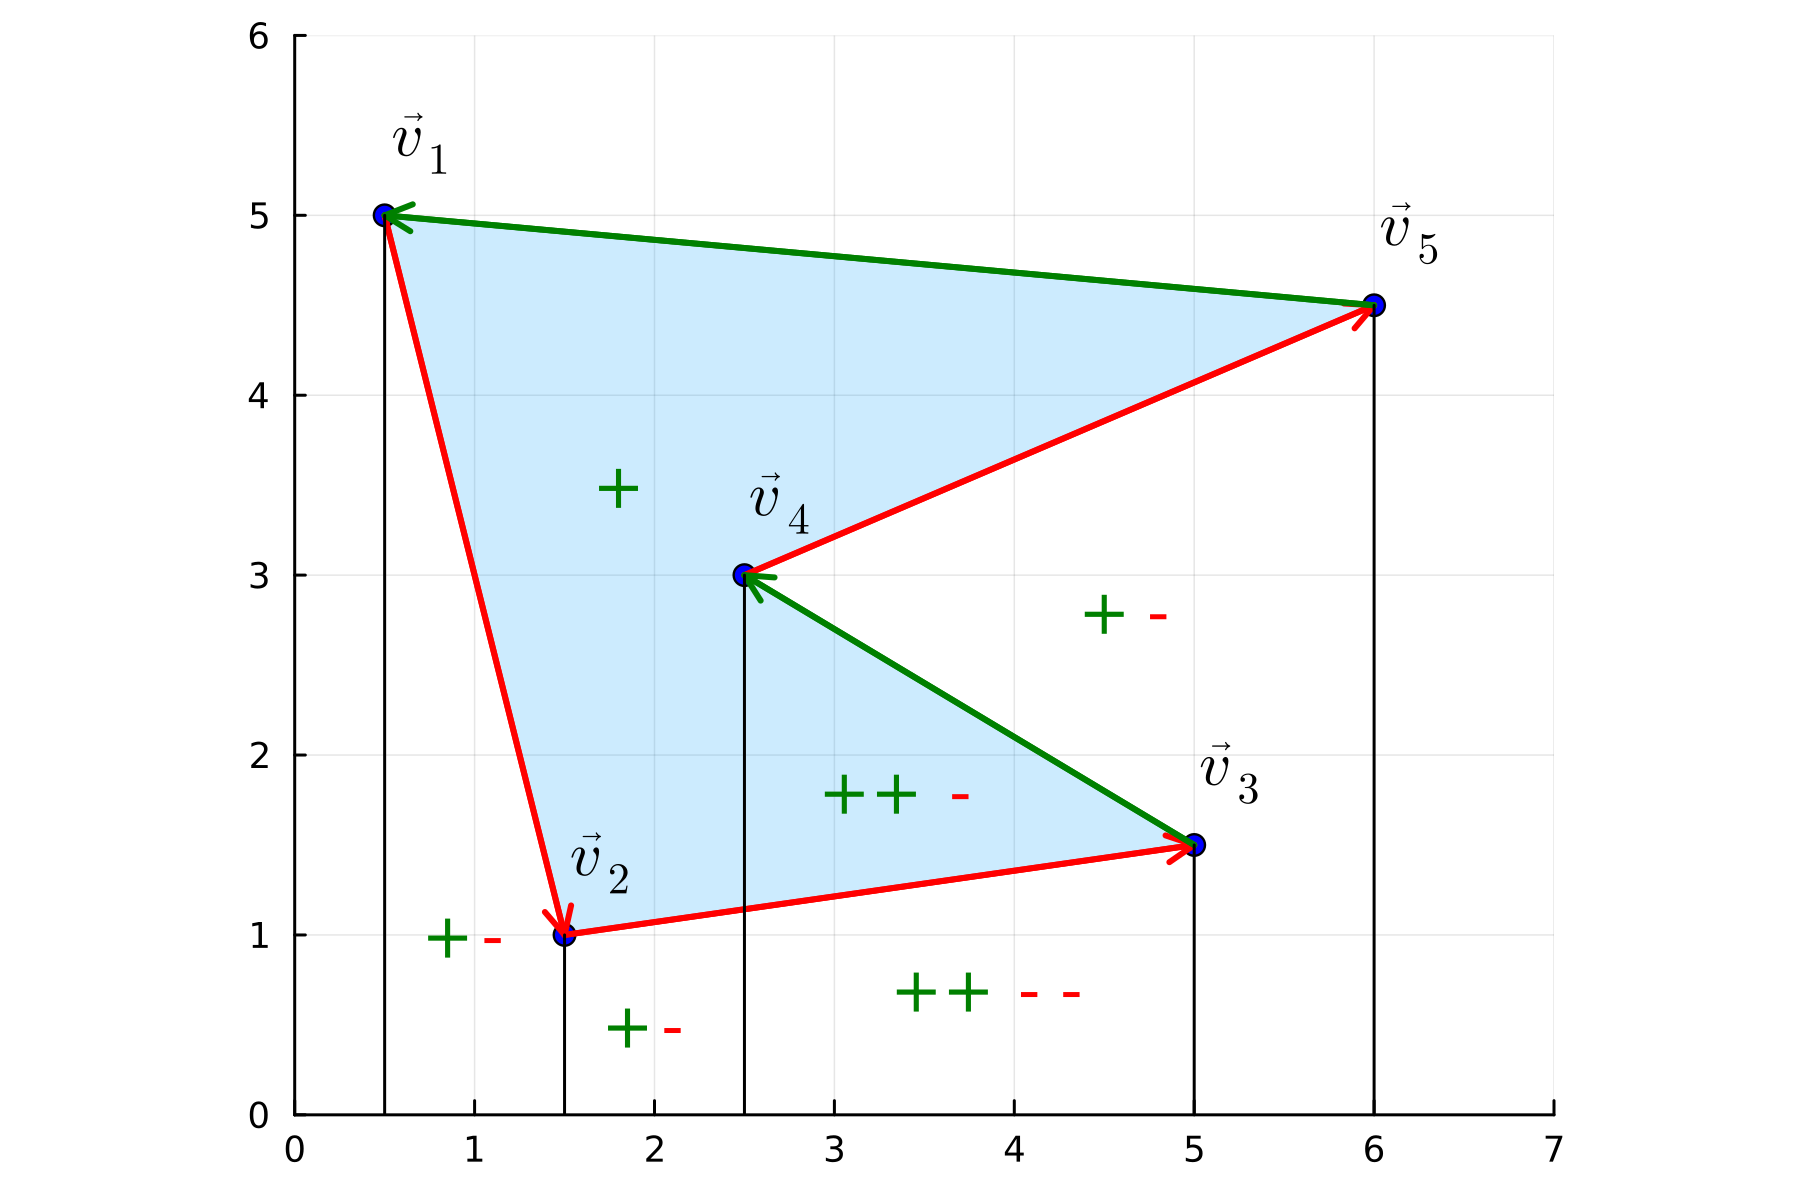
\includegraphics[width=8cm]{bachelors-thesis/shoelace_new.png}
			\caption{
				This figure shows a geometrical interpretation of the shoelace formula.
				The green arrows, which point from right to left, represent positive trapezoidal areas that contribute positively to the total area of the polygon.
				In contrast, the red arrows point from left to right and represent negative areas that are subtracted in the computation.
				The vertical black lines divide the plot into subregions.
				Within each subregion, green arrows are counted with plus signs and red arrows with minus signs.
				We observe that the subregions lying outside the polygon contain an equal number of plus and minus signs, indicating that their net contribution to the area is zero.
				In contrast, the subregions inside the polygon always have one more plus sign than minus signs, meaning their area is counted exactly once in the total.
				Overall, this illustrates that the method correctly computes the area of the polygon.
				Source:~\cite{ShoelaceFigure2022}}
			\label{fig:shoelace}
		\end{center}
	\end{figure}
	\qed
\end{proposition}

With the Shoelace formula we are able to easily compute all cell areas at all times in the simulation. 
This enables us to implement the gradient flow over the area energy. 

\begin{definition} \textbf{Area energy} \\
The energy $A_k: (\R^2)^{N_V} \rightarrow \R_{\geq 0}$ for $k \in \N_{\geq 1}$, used to keep the cells at a constant volume, reads 
	\begin{align}
		A_k(C) = \frac{1}{k} |A_{C} - A_d|^k, \label{eq:areaEnergy} 
	\end{align}
	where $A_d$ is the desired cell area of all cells and $A_{C}$ is the current area of cell $C$. 
\end{definition}

To maintain the cell area during the simulation, we evaluate the gradient flow of the area energy which indicates the direction of motion for each vertex for preserving the cell area.

\begin{proposition} \textbf{Area force} \label{force:area}\\
	The area force $F_{k}^{(A)}: (\R^2)^{N_V} \rightarrow (\R^2)^{N_V}$ that gets applied on cell $C$ is given by  
	\begin{align*}
		F_{k}^{(A)}(C) 
		= - (\nabla_{\vec{v}_1} A_k(C), \ldots, \nabla_{\vec{v}_{N_V}} A_k(C))^T,
	\end{align*}
	where the gradient $\nabla_{\vec{v}_j} A_k(C)$ with respect to $\vec{v}_j = (v_{j}^{x}, v_{j}^{y})^T$ is given by 
	\begin{align}
		\nabla_{\vec{v}_j} A_k(C) = \dfrac{1}{2} \sgn(A_{C} - A_d) |A_{C} - A_d|^{k-1} \begin{pmatrix} v_{j+1}^{y} - v_{j-1}^{y} \\[0.5em]  v_{j-1}^{x} - v_{j+1}^{x} \end{pmatrix},
		\label{gradient:area}
	\end{align}
	for all $1 \leq j \leq N_V$.\\


	Proof.\\
	Choose $1 \leq j \leq N_V$.  
 
	\begin{align*}
		\nabla_{\vec{v}_j} A_k(C) &= \frac{1}{k} \nabla_{\vec{v}_j} | A_{C} - A_d |^k  \\ 
		&= \sgn(A_{C} - A_d) | A_{C} - A_d |^{k-1} \nabla_{\vec{v}_j} (A_{C} - A_d) \\
		&= \sgn(A_{C} - A_d) | A_{C} - A_d |^{k-1} \nabla_{\vec{v}_j} A_{C} \\
		&= \sgn(A_{C} - A_d) | A_{C} - A_d |^{k-1} \nabla_{\vec{v}_j} \left(\frac{1}{2} \sum\limits_{k = 1}^{N} (v_k^{x} v_{k+1}^{y} - v_{k+1}^{x} v_k^{y})\right) \\[0.5em]  
		&= \frac{1}{2} \sgn(A_{C} - A_d) | A_{C} - A_d |^{k-1} \begin{pmatrix}
				\partial_{v_j^{x}} (v_j^{x} v_{j+1}^{y} - v_j^{x} v_{j-1}^{y})  \\[0.5em]
				\partial_{v_j^{y}} (v_{j-1}^{x} v_j^{y} - v_{j+1}^{x} v_j^{y})
			\end{pmatrix} \\[0.5em] 
		&= \frac{1}{2} \sgn(A_{C} - A_d) | A_{C} - A_d |^{k-1} \begin{pmatrix}
				v_{j+1}^{y} - v_{j-1}^{y}  \\
				v_{j-1}^{x}  - v_{j+1}^{x} 
			\end{pmatrix} 
	\end{align*}

	Remember that $A_d$ is just an independent constant. 
	\qed
\end{proposition}
It is also valid to write $F_{j}^{(A)}(\vec{C})$ instead of $F_{j}^{(A)}(C)$, since $C$ is included in $\vec{C}$. 


\begin{figure}[h!]
    \centering
    \begin{tabular}{cc}
        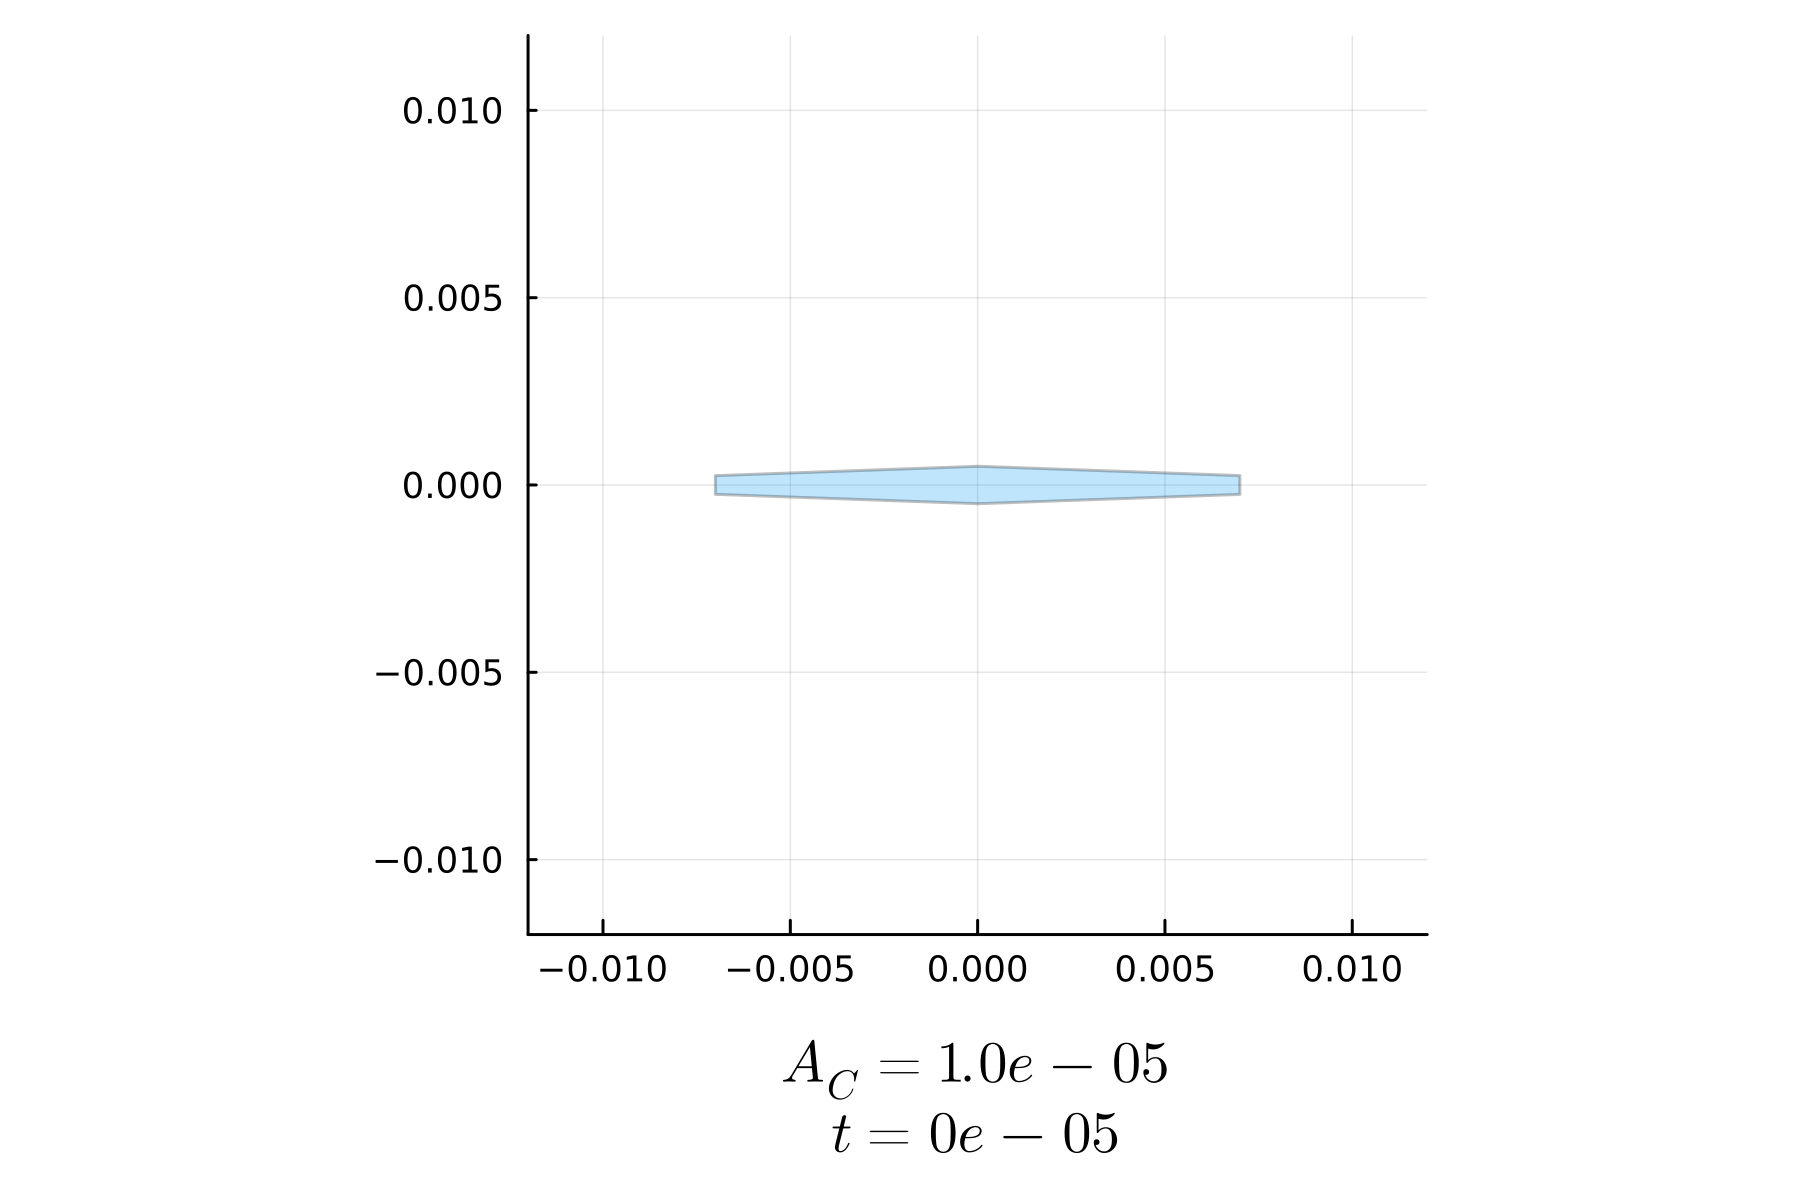
\includegraphics[width=0.5\textwidth]{forces/area1/t0.png} &
        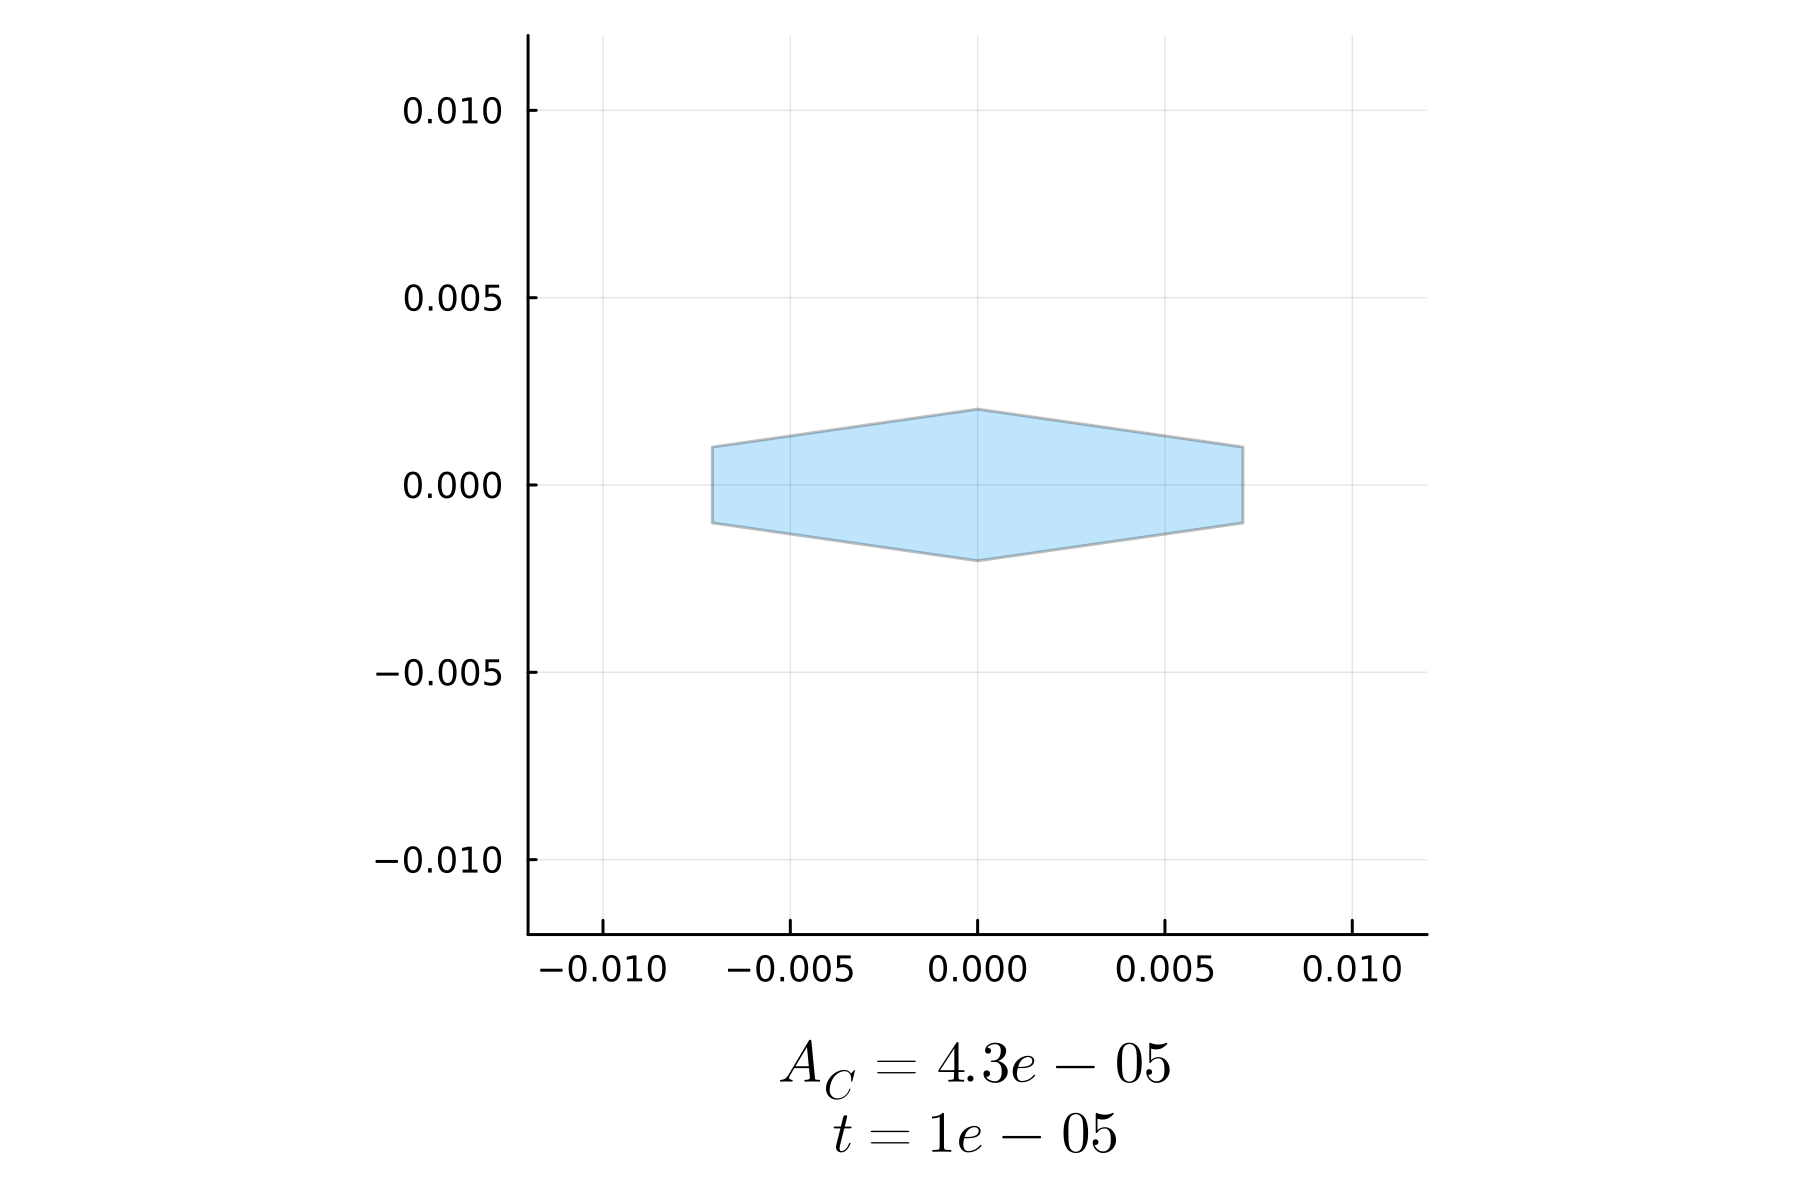
\includegraphics[width=0.5\textwidth]{forces/area1/t1.png} \\
        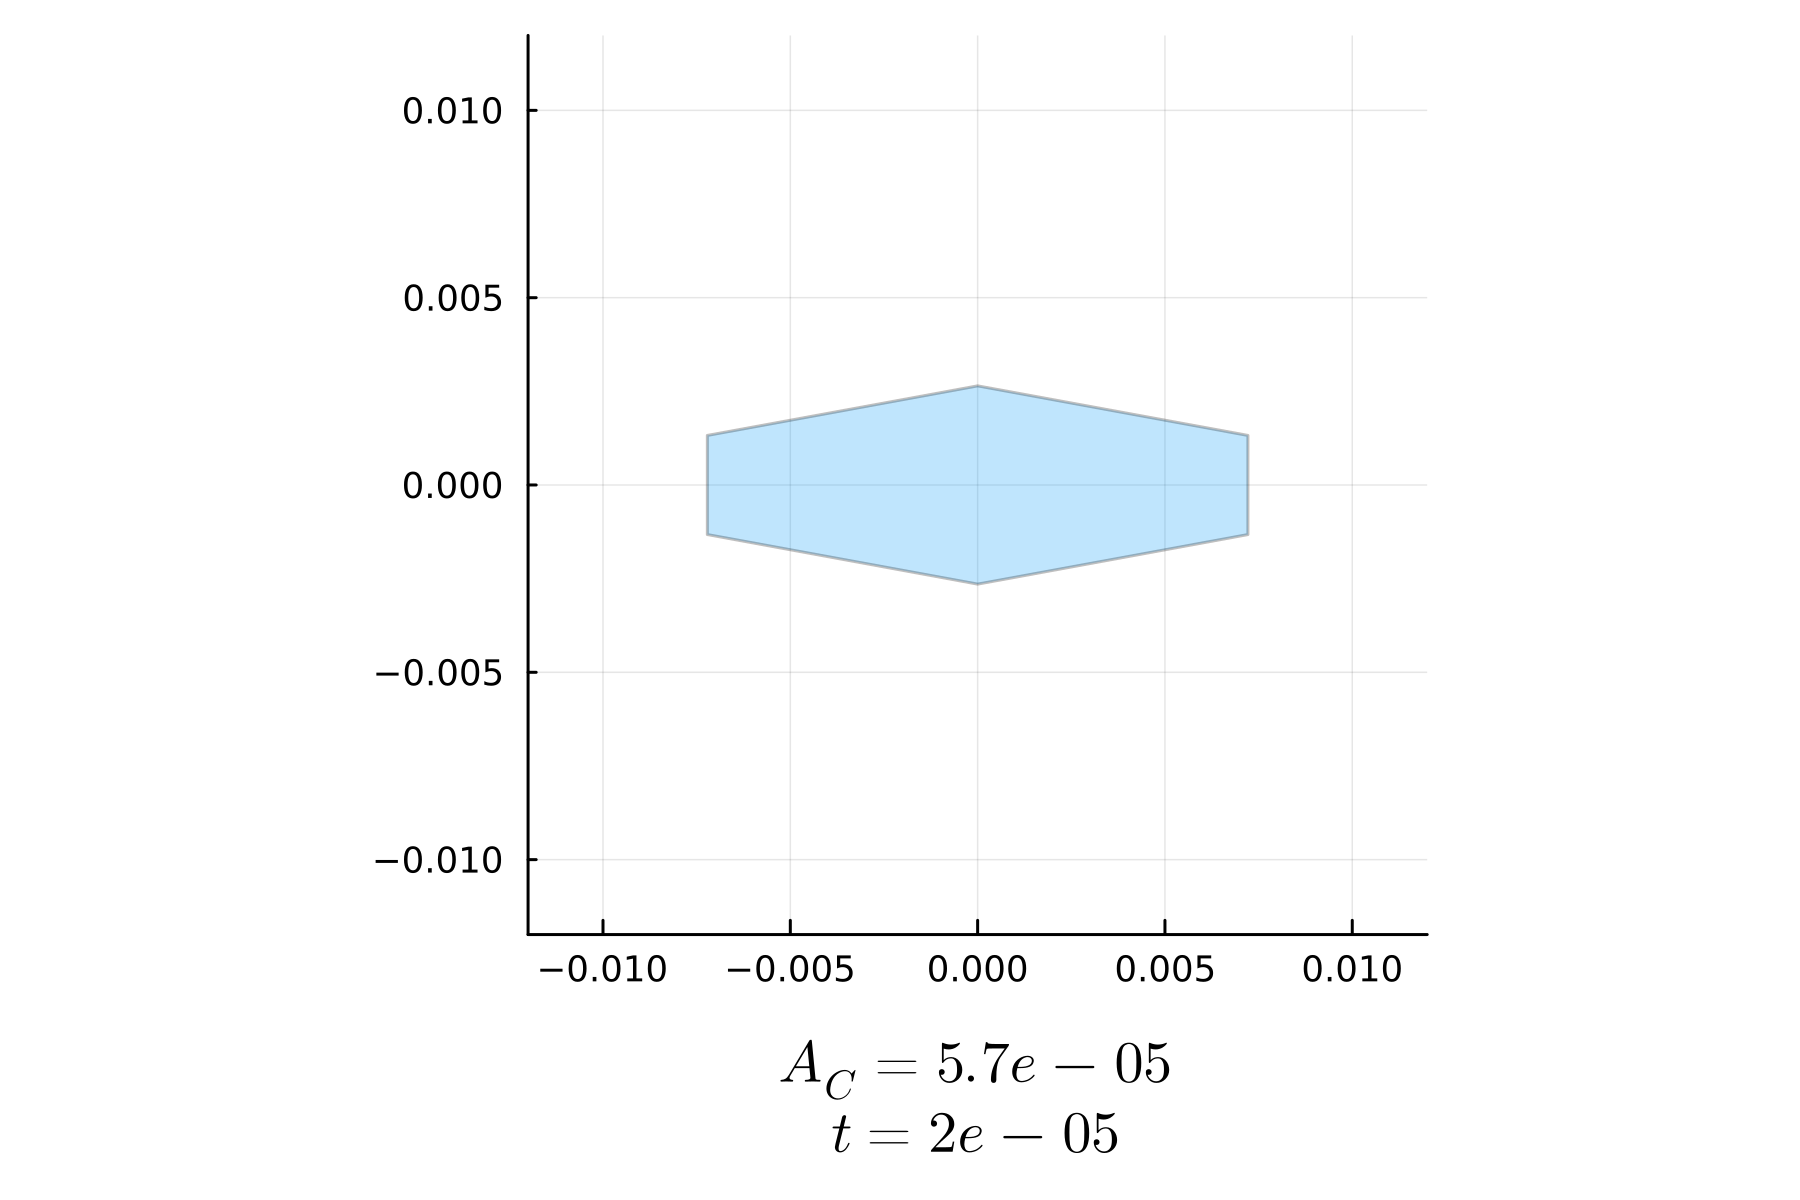
\includegraphics[width=0.5\textwidth]{forces/area1/t2.png} &
        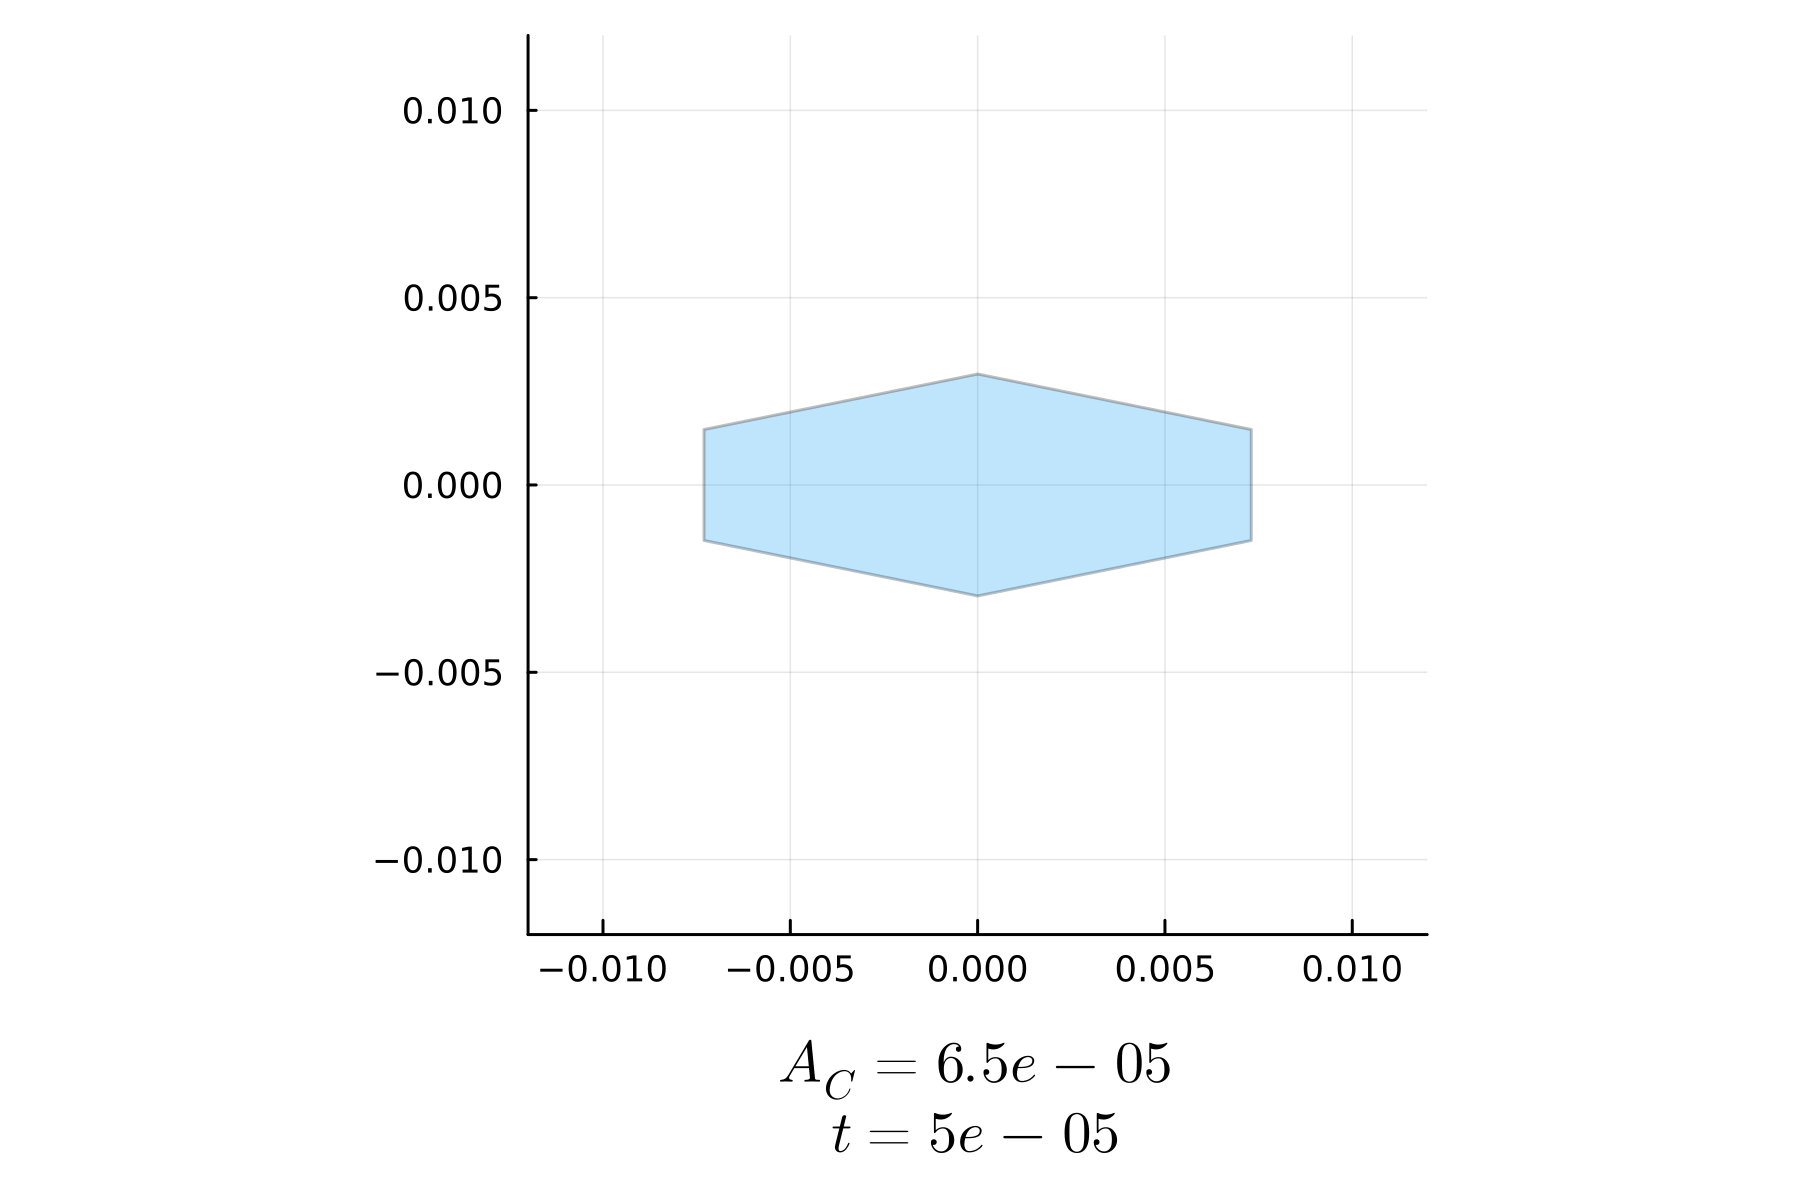
\includegraphics[width=0.5\textwidth]{forces/area1/t5.png} \\
    \end{tabular}
    \caption{The top four plots show the evolution of a DF cell influenced solely by the area force, with $k=2$ applied to the vertices and a force scaling of $4\times 10^{8}$, at times $t \in \{0, 1\times 10^{-5}, 2\times 10^{-5}, 5\times 10^{-5}\}$.\\
	Thus, we have $\frac{\dequ \vec{v}}{\dequ t} = - 4\times 10^{8} \nabla_{\vec{v}} A_2(C)$ for all vertices.
	The initial cell area is $A_C = 1\times 10^{-5}$, while the desired cell area is set to $6.5\times 10^{-5}$.\\
	We deliberately chose an irregular cell shape, since small vertical changes to the vertices lead to large changes in area.
	Click \href{https://github.com/tivo476c/FlexibleCellModel/blob/master/figures/gifs/showForces/show-areaForce.gif}{\textit{here}} to view the corresponding animation (GIF).\\
	The area force successfully restores the desired cell area after 5 time steps, which is also reflected Figure~\ref{fig:areaEnergyDiagram}.}
	\label{fig:areaForce}    
\end{figure}
\begin{figure}[h!]
    \centering
        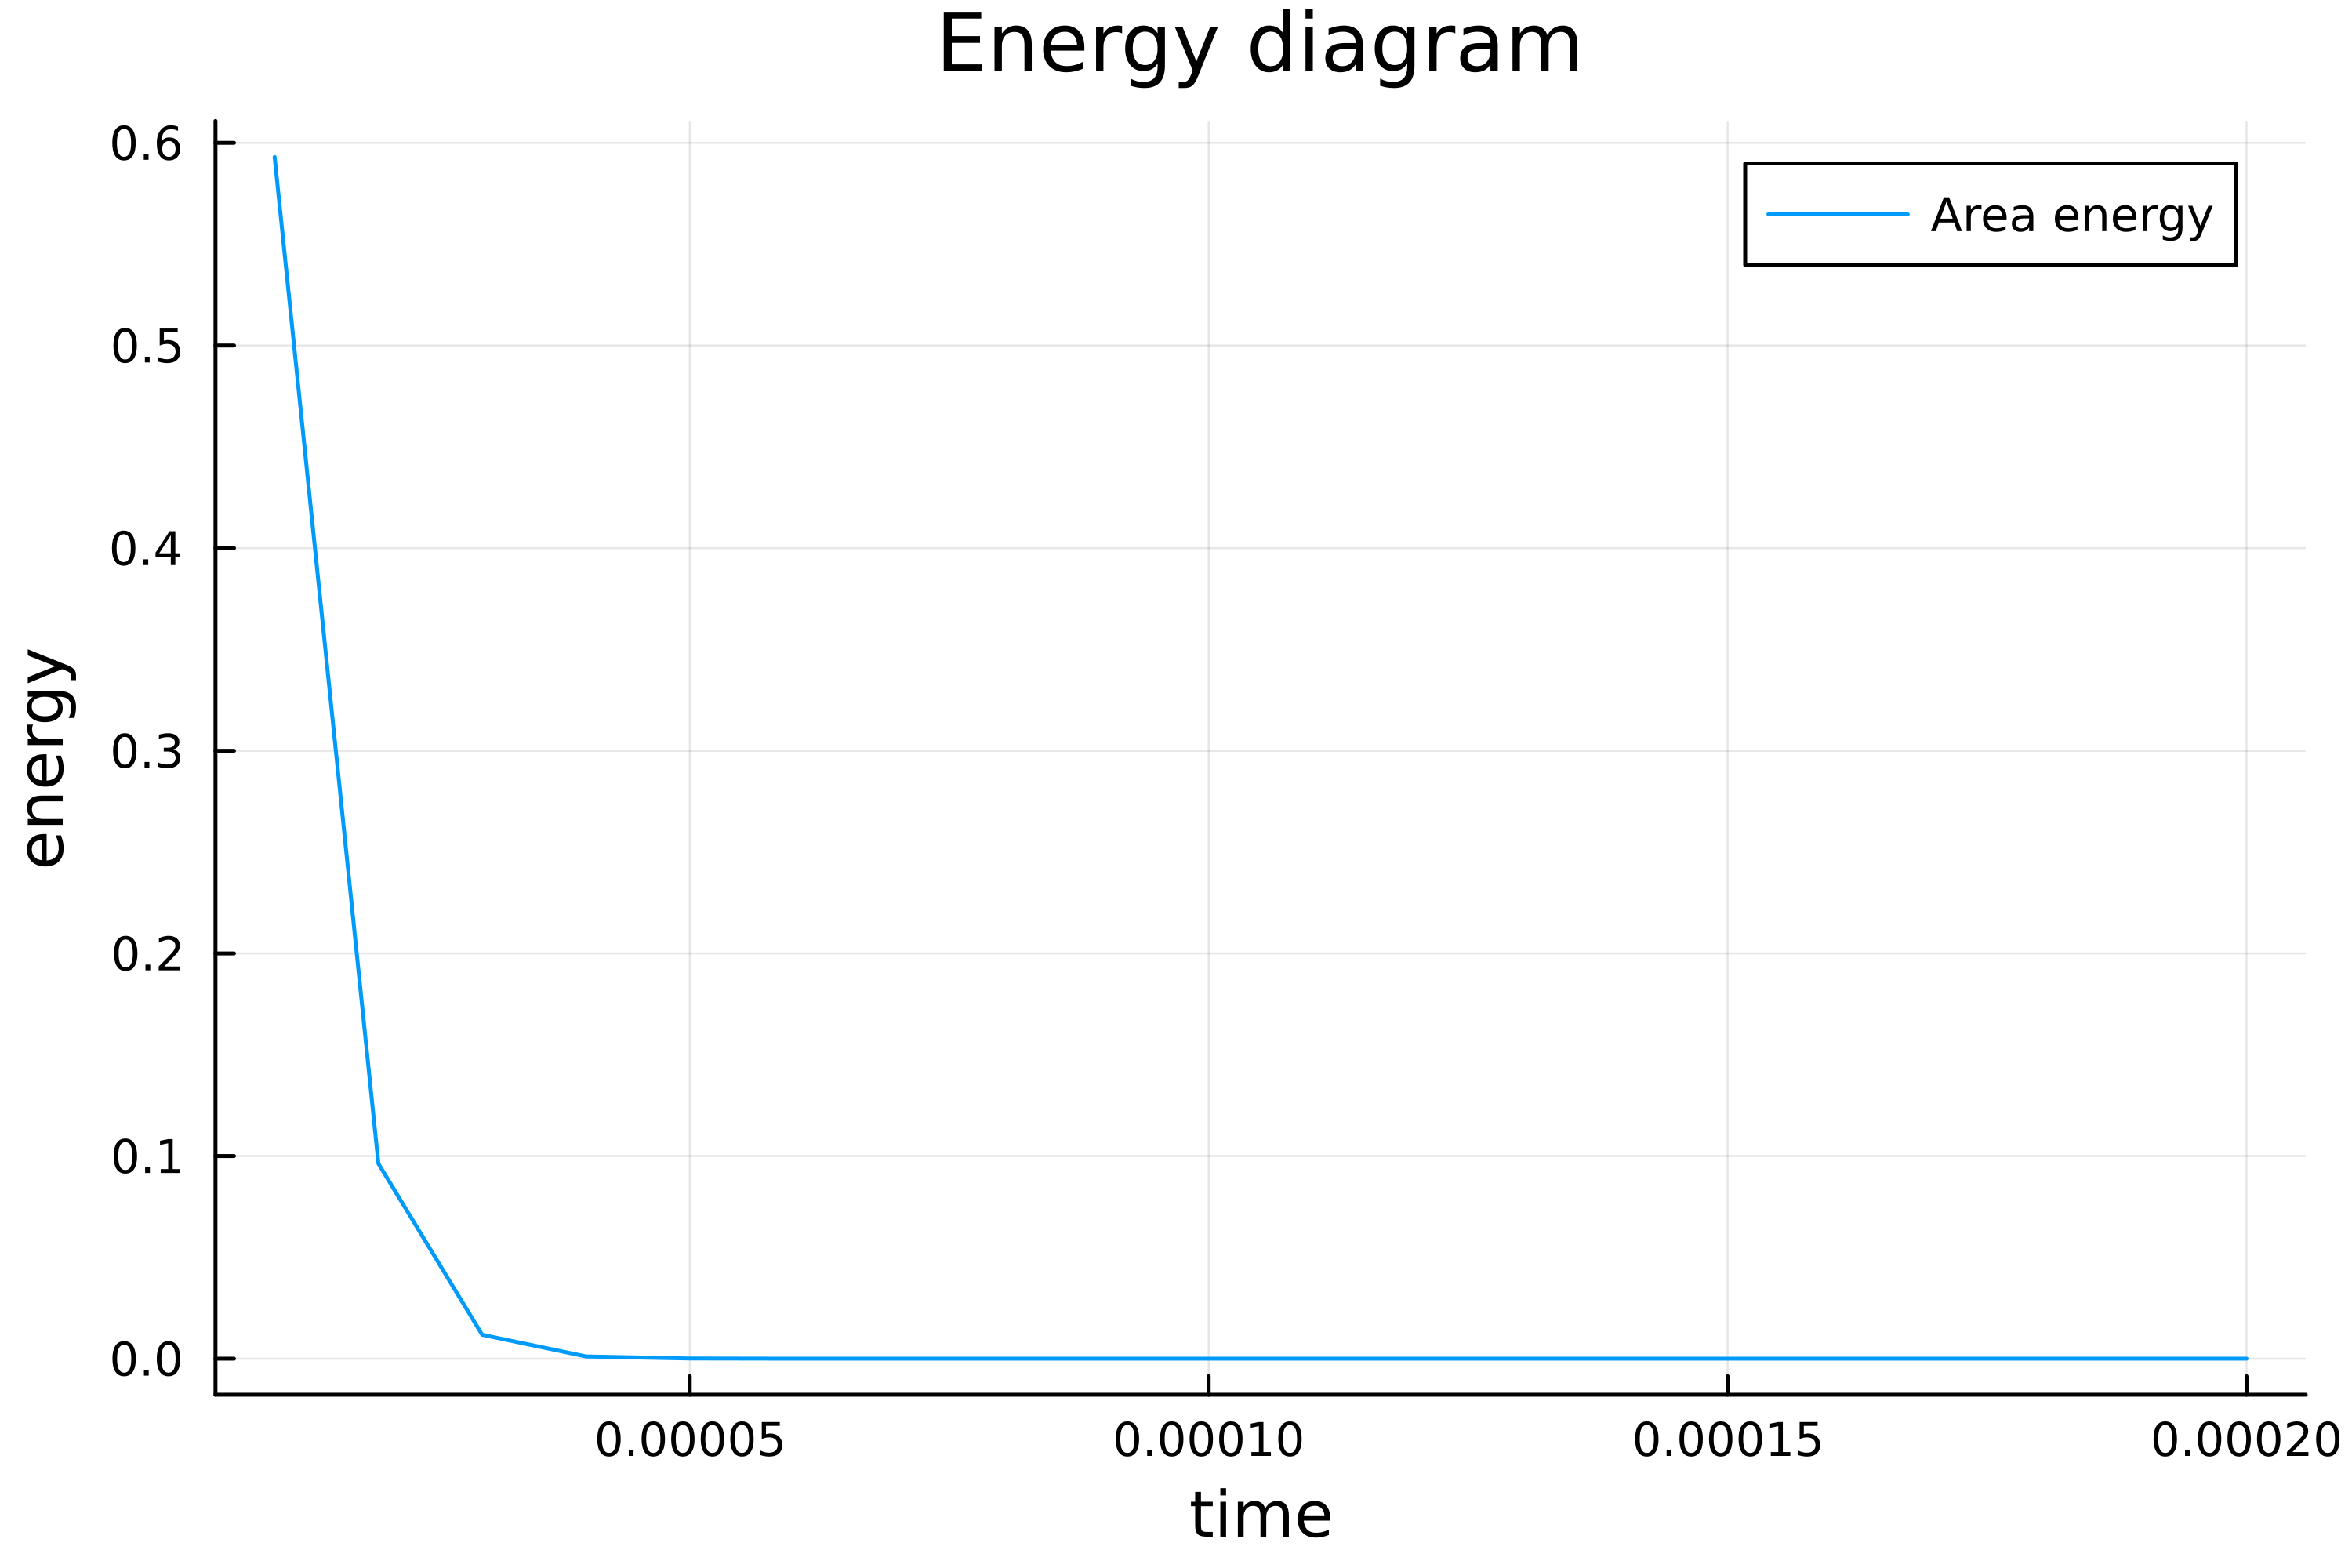
\includegraphics[width=0.7\textwidth]{forces/area1/energies-show-areaForce.png} 
    \caption{The area force successfully restores the desired cell area after 5 time steps as this energy diagram shows.}
	\label{fig:areaEnergyDiagram}    
\end{figure}
Figure~\ref{fig:areaForce} illustrates how the area force acts on a cell to either expand or contract it toward the desired target area.

    
\subsection{Edge force}
The next force we would like to model is the edge force. 
It acts on the cells' edges and aims to maintain their lengths.
We define the edge $1 \leq j \leq N_V$ as 
\begin{center}
	$
	e_j = \overline{\vec{v}_j \: \vec{v}_{j+1}}
	$
\end{center}
and we use the operator 
\begin{center}
	$
	E^j_C = \norm[\vec{v}_j - \vec{v}_{j+1}]
	$
\end{center}
to compute the length of the edge. 

The according energy for this edge is:
\begin{definition} \textbf{Edge energy} \\
	The energy $E_k: (\R^2)^{N_V} \rightarrow \R_{\geq 0}$, used to keep the edges at a constant length, reads 
	\begin{align}
		E_k(C) =  \sum\limits_{j=1}^{N_V} \frac{1}{k} |E^j_{C} - E^{j}_d|^k, \label{eq:edgeEnergy} 
	\end{align}
	where $E^j_{C}$ is the current edge length and $E^{j}_d$ is the desired edge length of edge $j$. 
\end{definition}

Since each vertex $\vec{v}_j$ influences exactly the edge lengths of the edges $e_{j}$ and $e_{j-1}$, we get the total edge force on $\vec{v}_j$ with: 

\begin{proposition} \textbf{Edge force} \\

	The edge force $F_{k}^{(E)}: (\R^2)^{N_V} \rightarrow (\R^2)^{N_V}$ that gets applied on cell $C$ is given by  
	\begin{align*}
		F_{k}^{(E)}(C) 
		= - (\nabla_{\vec{v}_1} E_k(C), \ldots, \nabla_{\vec{v}_{N_V}} E_k(C))^T,
	\end{align*}
	where the gradient $\nabla_{\vec{v}_j} E_k(C)$ with respect to $\vec{v}_j = (v_{j}^{x}, v_{j}^{y})^T$ is given by 
	\begin{align}
		\begin{split}
			\nabla_{\vec{v}_j} E_k(C) &= \sgn(E^{j-1}_{C}- E_d^{j-1}) \dfrac{|E^{j-1}_{C}- E_d^{j-1}|^{k-1}}{E^{j-1}_{C}}  
			\begin{pmatrix} v_{j}^{x} - v_{j-1}^{x} \\[0.5em]  v_{j}^{y} - v_{j-1}^{y}  \end{pmatrix} \\[0.5em]
			&+ \sgn(E^j_{C} - E_d^{j}) \dfrac{|E^j_{C} - E_d^{j}|^{k-1}}{E^j_{C}}  
			\begin{pmatrix} v_{j}^{x} - v_{j+1}^{x} \\[0.5em]  v_{j}^{y} - v_{j+1}^{y} \end{pmatrix}
		\end{split}
		\label{gradient:edge}
	\end{align}
	for all $1 \leq j \leq N_V$.\\

	Proof. \\

	\begin{align*}
		\nabla_{\vec{v}_{j}} E_k(C) &= \nabla_{\vec{v}_{j}} \sum\limits_{j=1}^{N_V} \frac{1}{k} |E^j_{C} - E^{j}_d|^k \\
		\nabla_{\vec{v}_{j}} E_k(C) &= \nabla_{\vec{v}_{j}} \sum\limits_{j=1}^{N_V} \frac{1}{k} |E^j_{C} - E^{j}_d|^k \\
		&= \frac{1}{k} \nabla_{\vec{v}_{j}} |E^{j-1}_{C} - E^{j-1}_d|^k + \frac{1}{k}\nabla_{\vec{v}_{j}} |E^j_{C} - E^{j}_d|^k 
	\end{align*}

	For the first summand, we can compute 
	\begin{align*}
		\frac{1}{k} \nabla_{\vec{v}_{j}} |E^{j-1}_{C} - E^{j-1}_d|^k 
		&= \sgn(E^{j-1}_C - E^{j-1}_d) |E^{j-1}_C - E^{j-1}_d|^{k-1} \nabla_{\vec{v}_j} (E^{j-1}_C - E^{j-1}_d) \\
		&= \sgn(E^{j-1}_C - E^{j-1}_d) |E^{j-1}_C - E^{j-1}_d|^{k-1} \nabla_{\vec{v}_j} E^{j-1}_C \\
		&= \sgn(E^{j-1}_C - E^{j-1}_d) |E^{j-1}_C - E^{j-1}_d|^{k-1} \cdot\\
		& \hspace{1cm} \nabla_{\vec{v}_j} [(v_{j-1}^{x} - v_{j}^{x})^2 + (v_{j-1}^{y} - v_{j}^{y})^2]^{\frac{1}{2}}\\
		&= \sgn(E^{j-1}_C - E^{j-1}_d) |E^{j-1}_C - E^{j-1}_d|^{k-1} \cdot    \\
		& \hspace{1cm} \left(\frac{1}{2 E^{j-1}_C} \nabla_{\vec{v}_j} [(v_{j-1}^{x} - v_{j}^{x})^2 + (v_{j-1}^{y} - v_{j}^{y})^2]\right) \\[0.5em] 
		&= \sgn(E^{j-1}_C - E^{j-1}_d) |E^{j-1}_C - E^{j-1}_d|^{k-1} \cdot\\
		& \hspace{1cm} \nabla_{\vec{v}_j} [(v_{j-1}^{x} - v_{j}^{x})^2 + (v_{j-1}^{y} - v_{j}^{y})^2]^{\frac{1}{2}}\\
		&= \sgn(E^{j-1}_C - E^{j-1}_d) |E^{j-1}_C - E^{j-1}_d|^{k-1} \cdot    \\
		& \hspace{1cm} \left(\frac{1}{2 E^{j-1}_C} \nabla_{\vec{v}_j} [(v_{j-1}^{x} - v_{j}^{x})^2 + (v_{j-1}^{y} - v_{j}^{y})^2]\right) \\[0.5em] 
		&= \sgn(E^{j-1}_C - E^{j-1}_d) \frac{|E^{j-1}_C - E^{j-1}_d|^{k-1}}{2 E^{j-1}_C} \begin{pmatrix}
			\partial_{v_{j}^{x}} (v_{j-1}^{x} - v_{j}^{x})^2 \\[0.5em]
			\partial_{v_{j}^{y}} (v_{j-1}^{y} - v_{j}^{y})^2
		\end{pmatrix} \\[0.5em]
		&= \sgn(E^{j-1}_C - E^{j-1}_d) \frac{|E^{j-1}_C - E^{j-1}_d|^{k-1}}{2 E^{j-1}_C} \begin{pmatrix}
			 -2(v_{j-1}^{x} - v_{j}^{x}) \\[0.5em]
			 -2(v_{j-1}^{y} - v_{j}^{y})
		\end{pmatrix} \\[0.5em] 
		&= \sgn(E^{j-1}_C - E^{j-1}_d) \frac{ |E^{j-1}_C - E^{j-1}_d|^{k-1}}{E^{j-1}_C} \begin{pmatrix}
				v_{j}^{x} - v_{j-1}^{x} \\[0.5em]
				v_{j}^{y} - v_{j-1}^{y}
		\end{pmatrix}
	\end{align*}

	For the second summand, we get:
	\begin{align*}
		\frac{1}{k} \nabla_{\vec{v}_{j}} |E^{j}_{C} - E^{j}_d|^k 
		&= \sgn(E^{j}_C - E^{j}_d) |E^{j}_C - E^{j}_d|^{k-1} \nabla_{\vec{v}_j} E^{j}_C \\
		&= \sgn(E^{j}_C - E^{j}_d) |E^{j}_C - E^{j}_d|^{k-1} \cdot   \\
		& \hspace{1cm} \left(\frac{1}{2 E^{j}_C} \nabla_{\vec{v}_j} [(v_{j}^{x} - v_{j+1}^{x})^2 + (v_{j}^{y} - v_{j+1}^{y})^2]\right) \\[0.5em] 
		&= \sgn(E^{j}_C - E^{j}_d) |E^{j}_C - E^{j}_d|^{k-1} \cdot   \\
		& \hspace{1cm} \left(\frac{1}{2 E^{j}_C} \nabla_{\vec{v}_j} [(v_{j}^{x} - v_{j+1}^{x})^2 + (v_{j}^{y} - v_{j+1}^{y})^2]\right) \\[0.5em] 
		&= \sgn(E^{j}_C - E^{j}_d) \frac{|E^{j}_C - E^{j}_d|^{k-1}}{2 E^{j}_C} \begin{pmatrix}
			\partial_{v_{j}^{x}} (v_{j}^{x} - v_{j+1}^{x})^2 \\[0.5em]
			\partial_{v_{j}^{y}} (v_{j}^{y} - v_{j+1}^{y})^2
		\end{pmatrix} \\[0.5em]
		&= \sgn(E^{j}_C - E^{j}_d) \frac{|E^{j}_C - E^{j}_d|^{k-1}}{2 E^{j}_C} \begin{pmatrix}
			2(v_{j}^{x} - v_{j+1}^{x}) \\[0.5em]
			2(v_{j}^{y} - v_{j+1}^{y})
		\end{pmatrix} \\[0.5em]
		&= \sgn(E^{j}_C - E^{j}_d) \frac{ |E^{j}_C - E^{j}_d|^{k-1}}{E^{j}_C} \begin{pmatrix}
				v_{j}^{x} - v_{j+1}^{x} \\[0.5em]
				v_{j}^{y} - v_{j+1}^{y}
		\end{pmatrix}
	\end{align*}
	
	\qed  
\end{proposition}

An isolated application of the edge force can be seen in Figure~\ref{fig:edgeForce}.  

\begin{figure}[h!]
    \centering
    \begin{tabular}{cc}
        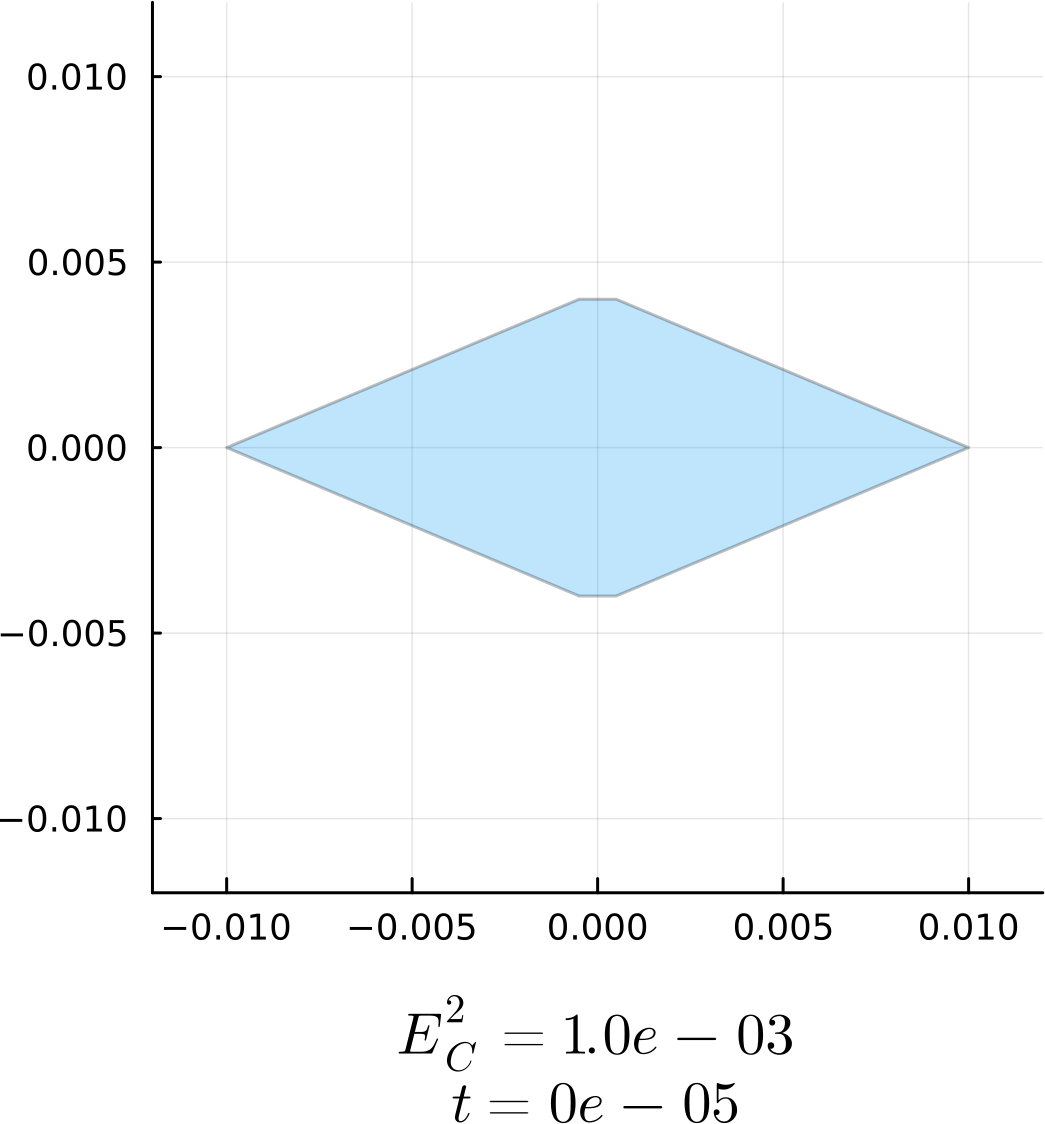
\includegraphics[width=0.5\textwidth]{forces/edge1/t0.png} &
        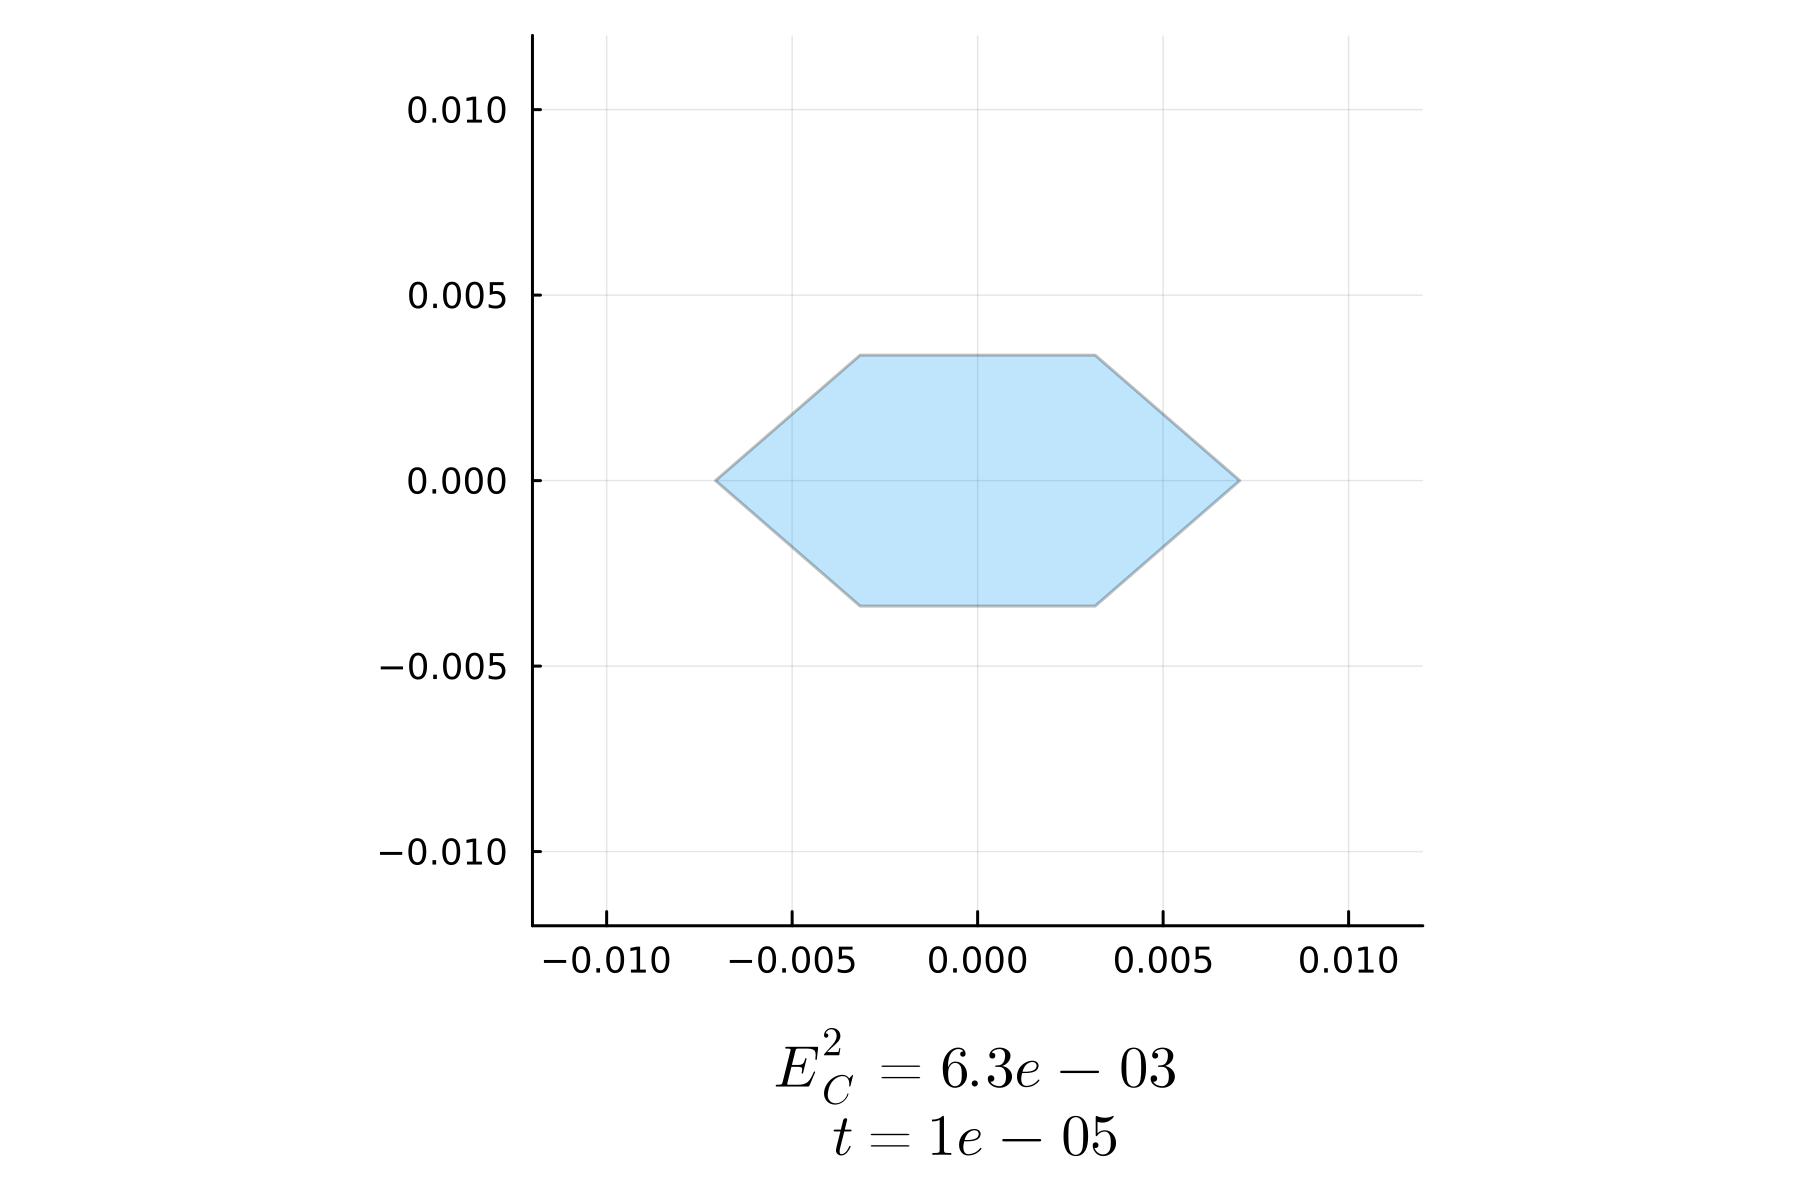
\includegraphics[width=0.5\textwidth]{forces/edge1/t1.png} \\
        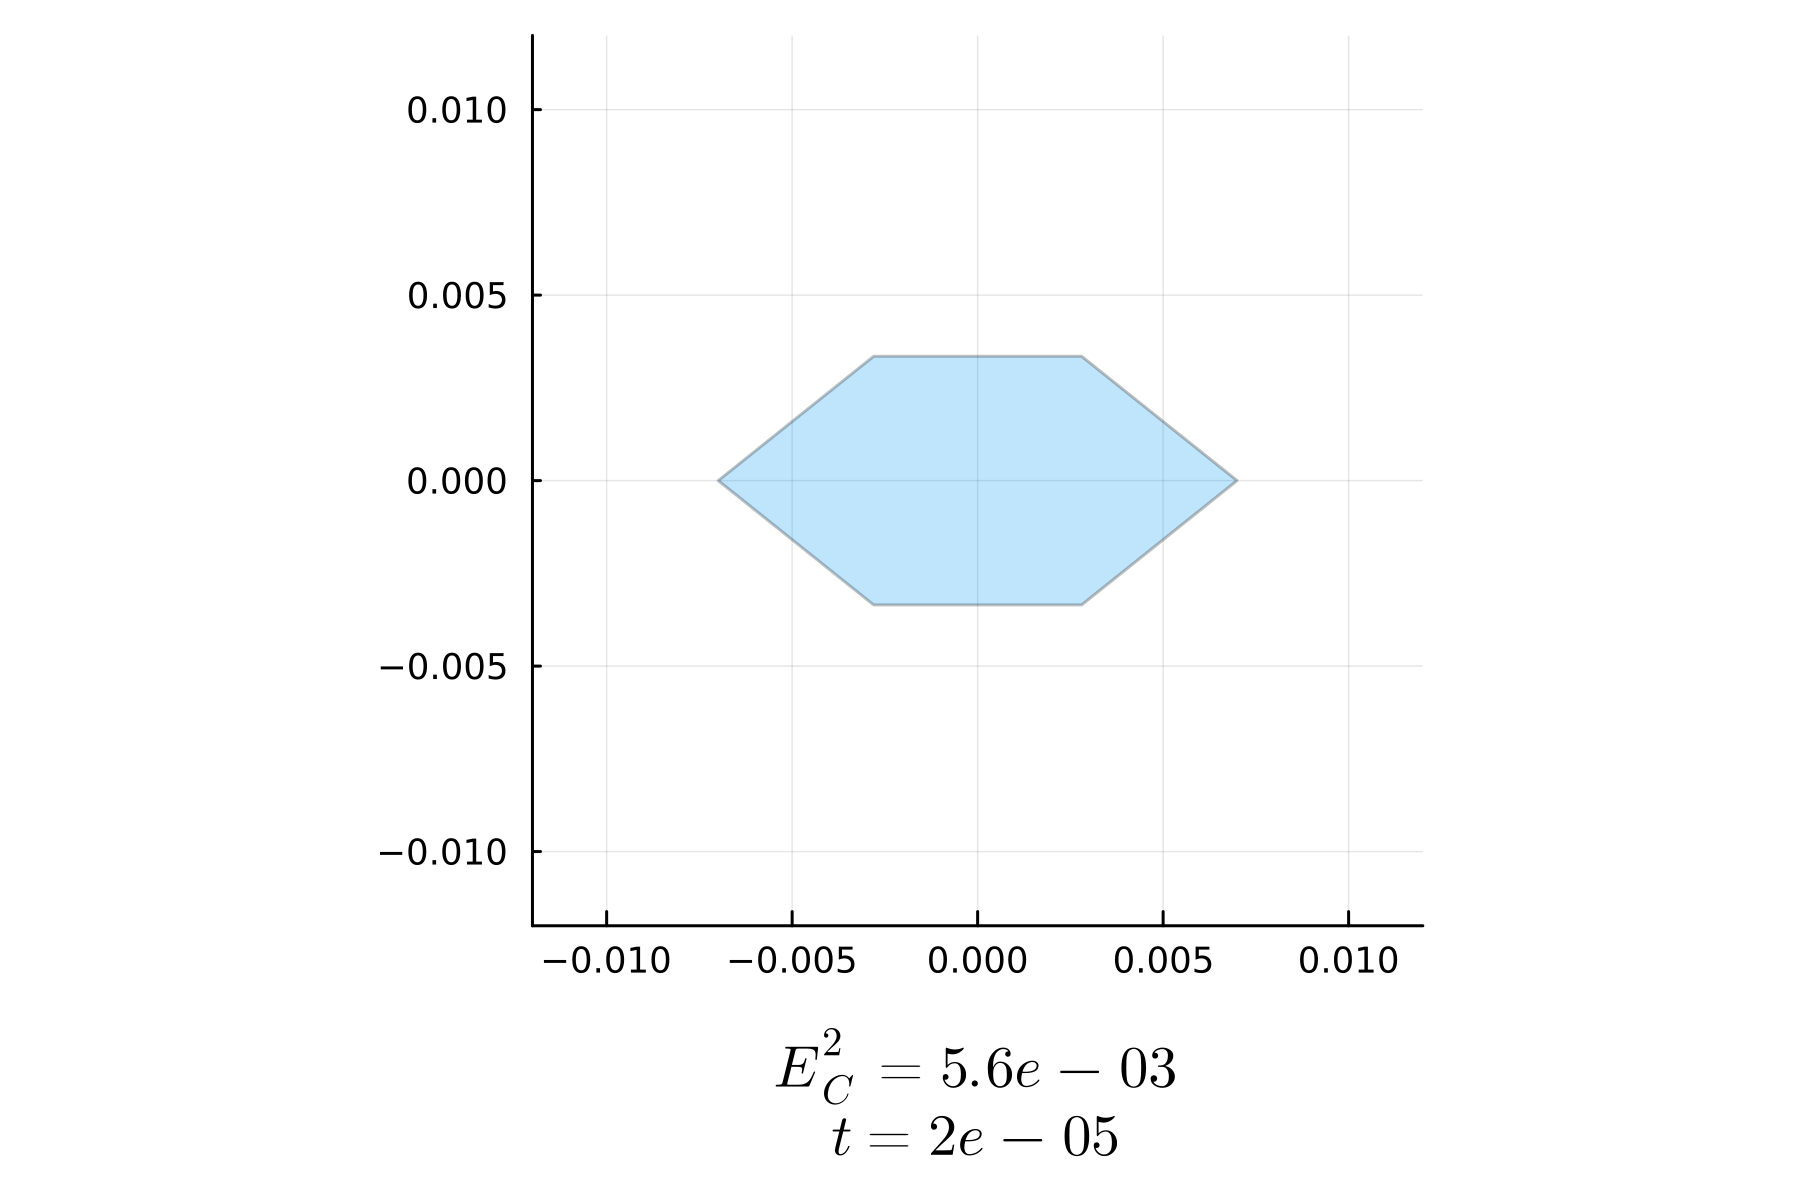
\includegraphics[width=0.5\textwidth]{forces/edge1/t2.png} &
        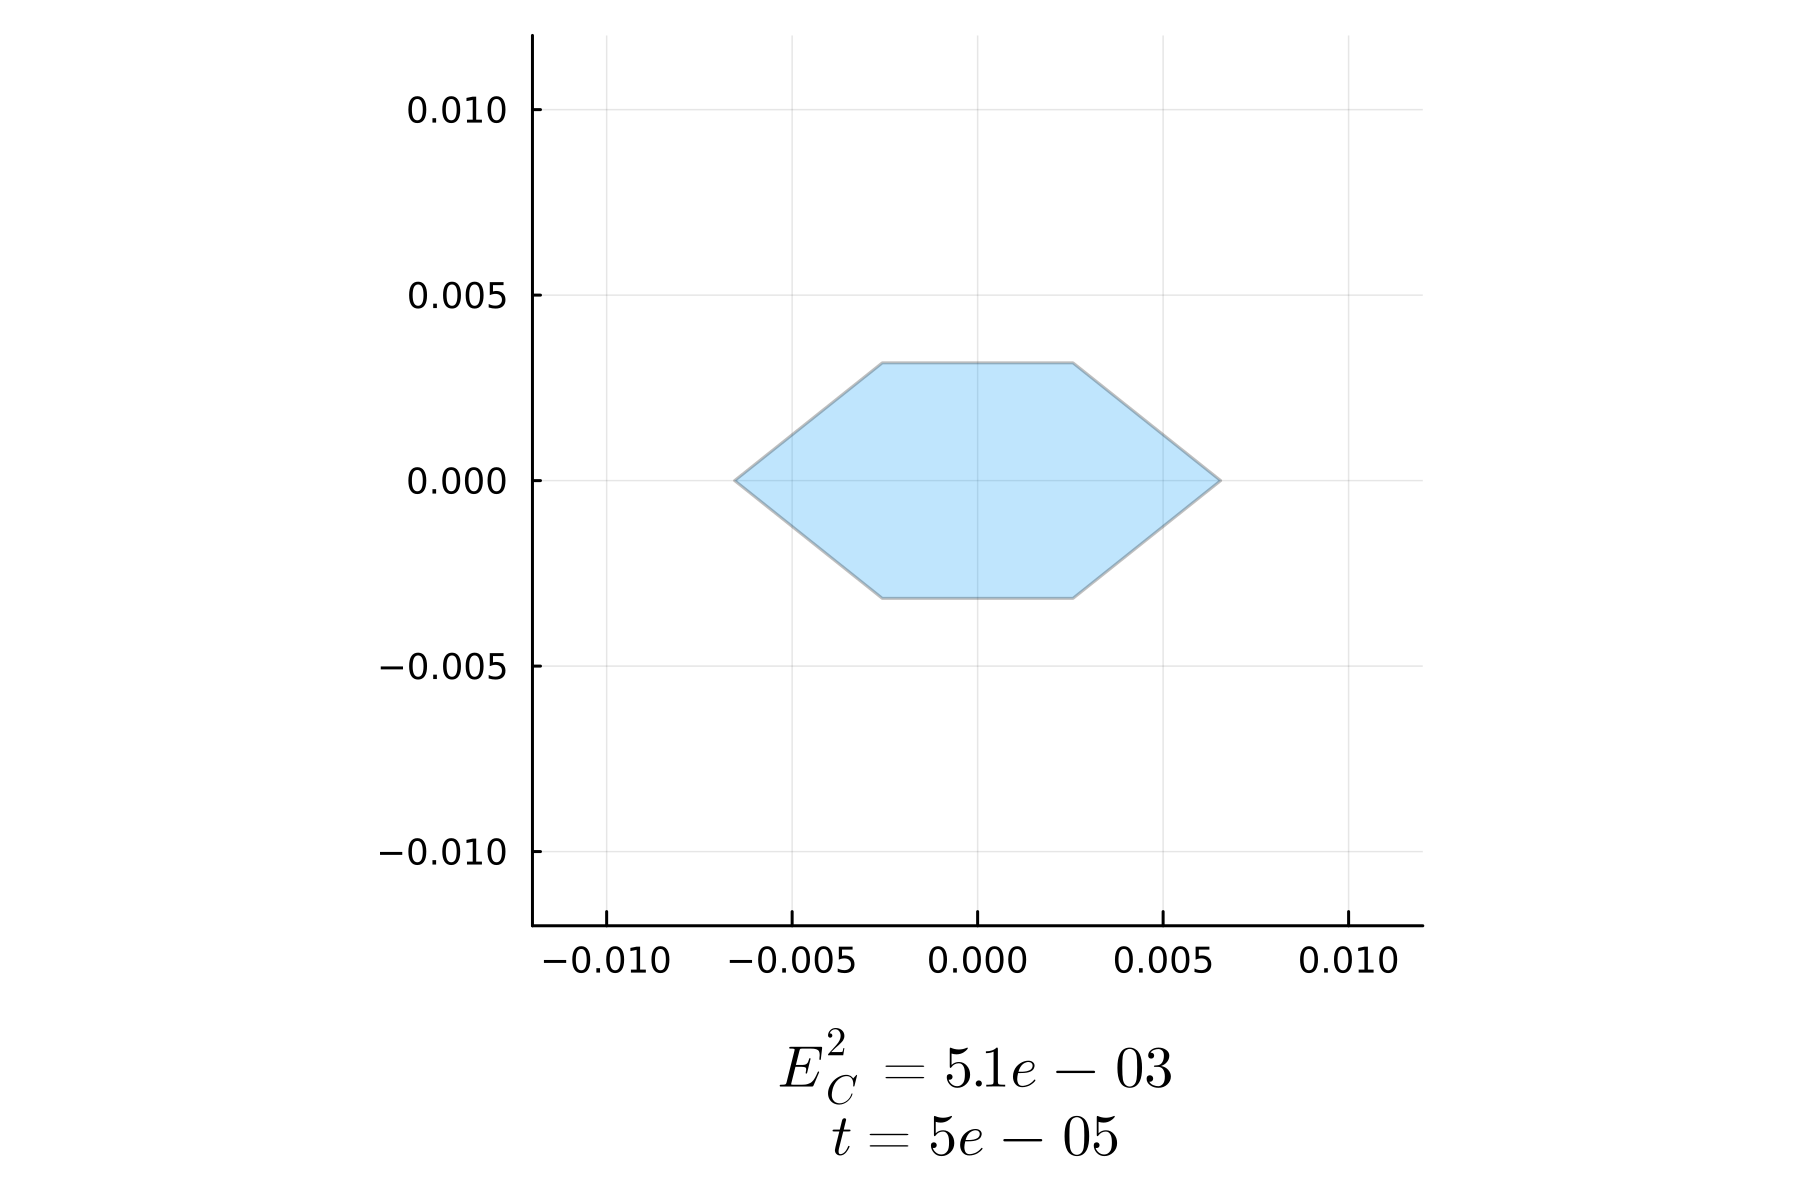
\includegraphics[width=0.5\textwidth]{forces/edge1/t5.png} \\
    \end{tabular}
    \caption{The top figures illustrate the evolution of a DF cell governed exclusively by the edge force, with $k=2$ applied to the vertices and a force scaling of $3\times 10^{4}$, at times $t \in \{0, 1\times 10^{-5}, 2\times 10^{-5}, 5\times 10^{-5}\}$.\\
		Accordingly, we have $\frac{\dequ \vec{v}}{\dequ t} = - 3\times 10^{4} \nabla_{\vec{v}} E_2(C)$ for all vertices.\\
		The initial edge length of the top edge is $E_C^2 = 1\times 10^{-3}$, while the desired edge lengths are all set to $5\times 10^{-3}$.\\
		Click \href{https://github.com/tivo476c/FlexibleCellModel/blob/master/figures/gifs/showForces/show-edgeForce.gif}{\textit{here}} to view the associated animation (GIF).\\
		The edge force nearly restores the desired edge lengths after 5 time steps, which can also be observed in Figure~\ref{fig:edgeEnergyDiagram}.
		}
		\label{fig:edgeForce}
\end{figure}
\begin{figure}[h!]
    \centering
        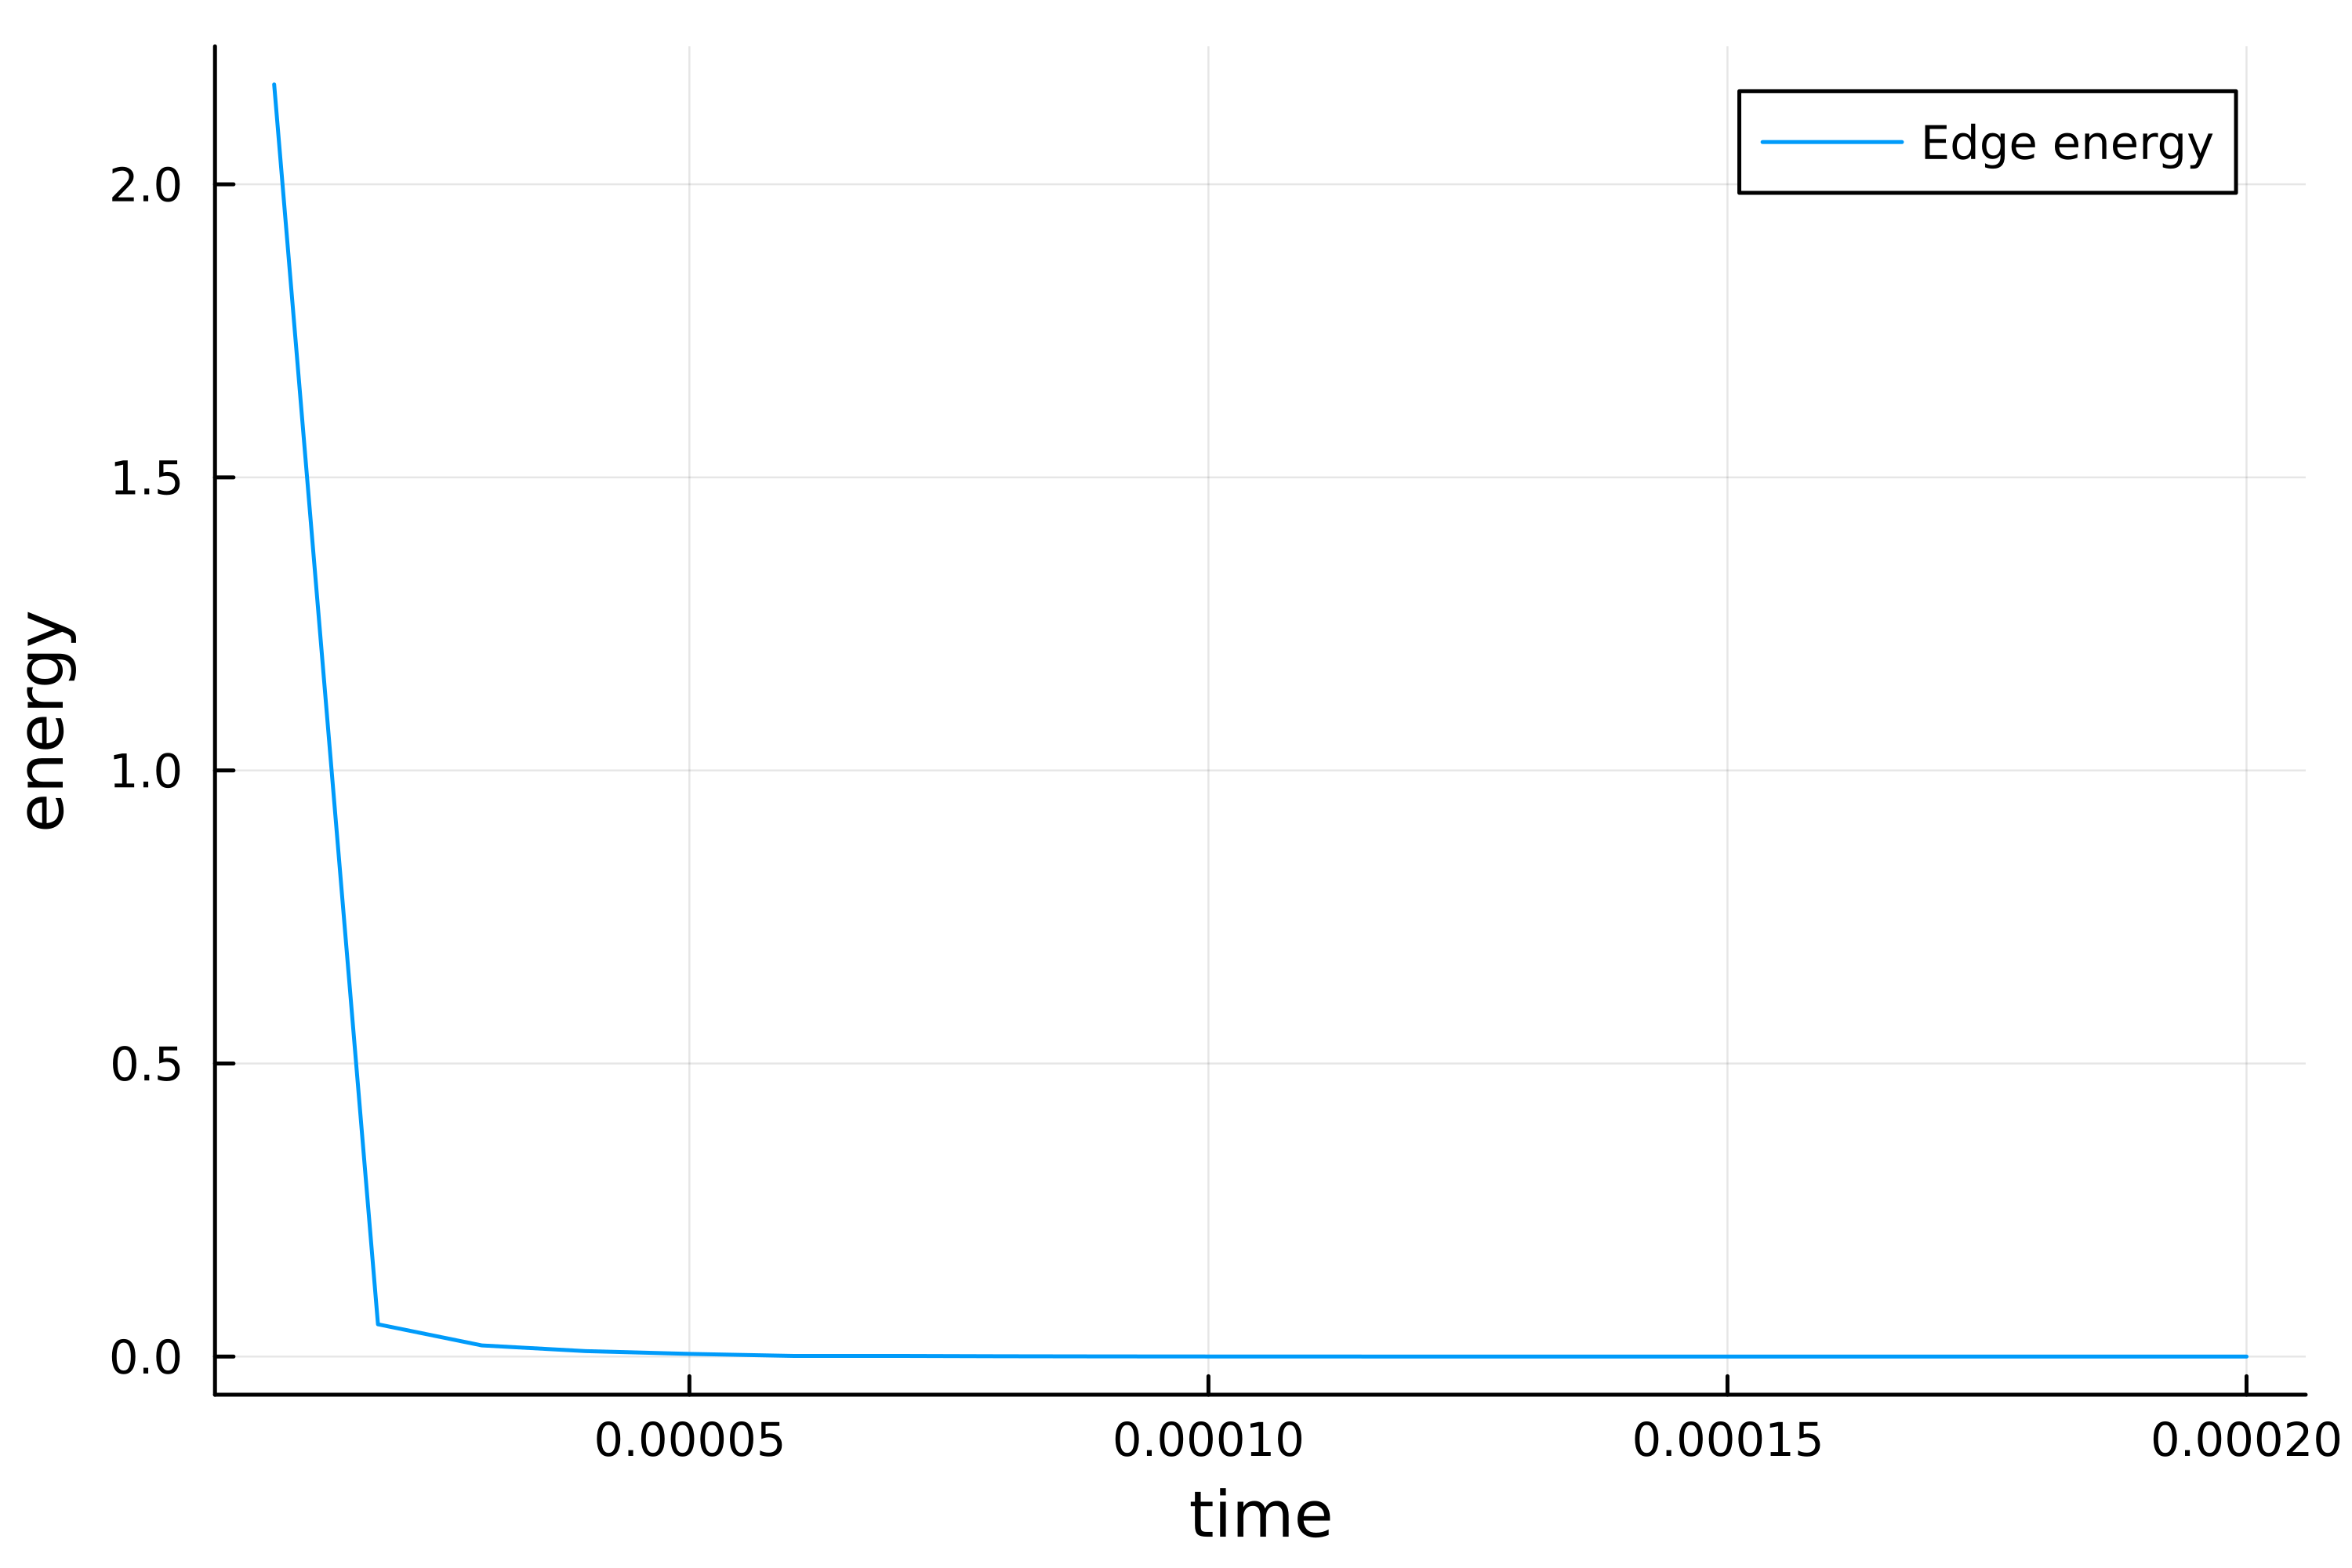
\includegraphics[width=0.7\textwidth]{forces/edge1/energies-show-edgeForce.png} 
    \caption{This energy diagram shows that the edge force nearly restores the desired edge lengths after 5 time steps.}
	\label{fig:edgeEnergyDiagram}    
\end{figure}

\subsection{Interior angle force}
% mention scaling factor of /360 for interior angle force 
The combined application of the area and edge forces revealed instabilities in unfavorable configurations, where self-intersections of the cell edges occurred. 
Simulations without this energy sometimes can also result in constrictions at certain vertices, where the interior angle approaches $360$°. 
To address this issue, we introduce the interior angle energy. \\
The first challenge is to consistently determine the interior angle at a given vertex throughout the simulation.
Although we could apply the law of cosines and use $\arccos$ to compute the angle, this method would suffer from poor stability as the angle approaches $180$°.
A better alternative is to use the $\atanxy$ function, as it remains reliably stable at all angles. \\

\begin{definition} \textbf{arctan2} \\
	The function $$\atanxy:\R^2/\{0\} \rightarrow (-\pi, \pi]$$ is defined by:
	\begin{center}
		$ \atanxy(\vec{v}) = 
		\begin{cases}
			\arctan(\frac{v^{y}}{v^{x}}) & v^{x} > 0 \\
			\arctan(\frac{v^{y}}{v^{x}}) + \pi & v^{x} < 0, v^{y} > 0 \\
			\arctan(\frac{v^{y}}{v^{x}}) - \pi & v^{x} < 0, v^{y} < 0 \\
			\pi & v^{x} < 0, v^{y} = 0 \\
			\dfrac{\pi}{2} & v^{x} = 0, v^{y} > 0 \\ 		
			- \dfrac{\pi}{2} & v^{x} = 0, v^{y} < 0 \\ 
		\end{cases}. $
	\end{center}
\end{definition}

The $\atanxy(\vec{v})$ function computes the angle of a vector $\vec{v}$ with respect to the positive $x$ axis. \\
With this, we can compute the angles 
\begin{center}
	
	$\theta_1 = \atanxy( \vec{v}_{j-1} - \vec{v_j} )$, \\
	$\theta_2 = \atanxy( \vec{v}_{j+1} - \vec{v_j} )$
	
\end{center}
between the positive $x$ axis and the vectors from $\vec{v}_j$ to its neighboring vertices $\vec{v}_{j-1}$ and $\vec{v}_{j+1}$. 
We get the searched angle at $\vec{v}_j$ by subtracting $\theta_1 - \theta_2$.
To ensure that the angle lies within the interval $[0, 2\pi)$, we use the modulo operator $[ \cdot ]_{[0,2\pi)}$, which repeatedly adds or subtracts $2\pi$ from the angle until it falls within the desired range.
Thus, our interior angle operator is: 
\begin{center}
	$
	I^j_C = [\atanxy(\vec{v}_{j-1} - \vec{v_j}) - \atanxy(\vec{v}_{j+1} - \vec{v_j})]_{[0,2\pi)}.
	$
\end{center}

With that, we can define our interior angle energy. 
\begin{definition} \textbf{Interior angle energy} \\
	The energy $I: (\R^2)^{N_V} \rightarrow \R_{\geq 0}$ associated with preserving the cell interior angles is given by
	\begin{align}
		I_k(C) = \sum\limits_{j=1}^{N_V} \frac{1}{k}| I^j_{C} - I^{j}_d |^k, 
	\end{align}
	where $I^{j}_d$ is the desired interior angle at vertex $j$ and $I^j_{C}$ is the current interior angle at vertex $j$ of the considered cell. 
\end{definition}


We continue by computing the resulting force. 
The $\atanxy$ function is partly defined and not truly differentiable. 
We still want to compute a gradient to use it for our interior angle force. 
It is $$\atanxy(\vec{v}) = \arctan\!\left(\frac{v^{y}}{v^{x}} \right) + \text{constant}$$ almost everywhere, just not on areas with measure zero. 
We just compute the gradient of $\arctan(\frac{v^{y}}{v^{x}})$ instead. \\
Another problem is the modulo operator $[ \cdot ]_{[0,2\pi)}$, which is not differentiable at the interval limits.
However, we just neglect the modulo operator as it does not affect the dynamics of the gradient.

\begin{proposition} \textbf{Interior angle force} \\

	% The interior angle force $F^{(I)}_j(C): (\R^2)^{N_V} \rightarrow \R^2$ that gets applied on vertex $\vec{v}_j$ of cell $C$ is given by 
	% \begin{align}
	% 	\begin{split}
	% 		F^{(I)}_j(C) &= - \nabla_{\vec{v}_j} I(C)  \\
	% 			&= (I^{j-1}_d - I^{j-1}_{C}) \left( 
	% 				- \frac{1}{\norm[\vec{v}_{j} - \vec{v}_{j-1}]^{y}} \begin{pmatrix}
	% 					v_{j}^{y} - v_{j-1}^{y} \\[0.5em]
	% 					v_{j-1}^{x} - v_{j}^{x}
	% 				\end{pmatrix} 
	% 			\right) \\[0.5em] 
	% 		&+ (I^{j}_d - I^{j}_{C}) \left( 
	% 			\frac{1}{\norm[\vec{v}_{j-1} - \vec{v}_j]^{y}} \begin{pmatrix}
	% 			v_{j-1}^{y} - v_{j}^{y} \\[0.5em]
	% 			v_{j}^{x} - v_{j-1}^{x}
	% 			\end{pmatrix} 
	% 			- \frac{1}{\norm[\vec{v}_{j+1} - \vec{v}_j]^2} \begin{pmatrix}
	% 			v_{j+1}^{y} - v_{j}^{y} \\[0.5em]
	% 			v_{j}^{x} - v_{j+1}^{x}
	% 			\end{pmatrix} 
	% 			\right) \\[0.5em] 
	% 		&+ (I^{j+1}_d - I^{j+1}_{C}) \left( 
	% 			\frac{1}{\norm[\vec{v}_{j} - \vec{v}_{j+1}]^2} \begin{pmatrix}
	% 			v_{j}^{y} - v_{j+1}^{y} \\[0.5em]
	% 			v_{j+1}^{x} - v_{j}^{x}
	% 			\end{pmatrix} 
	% 			\right) %\\[0.5em] 
	% 	\end{split}
	% \end{align}

	The interior angle force $F_{k}^{(I)}: (\R^2)^{N_V} \rightarrow (\R^2)^{N_V}$ that gets applied on cell $C$ is given by  
	\begin{align*}
		F_{k}^{(I)}(C) 
		= - (\nabla_{\vec{v}_1} I_k(C), \ldots, \nabla_{\vec{v}_{N_V}} I_k(C))^T,
	\end{align*}
	where the gradient $\nabla_{\vec{v}_j} I_k(C)$ with respect to $\vec{v}_j = (v_{j}^{x}, v_{j}^{y})^T$ is given by 
	\begin{align}
		\begin{split}
			\nabla_{\vec{v}_j} I_k(C) &= \sgn(I^{j-1}_{C} - I^{j-1}_d) |I^{j-1}_{C} - I^{j-1}_d|^{k-1} \left( 
					- \frac{1}{\norm[\vec{v}_{j} - \vec{v}_{j-1}]^{2}} \begin{pmatrix}
						v_{j-1}^{y} - v_{j}^{y} \\[0.5em]
						v_{j}^{x} - v_{j-1}^{x}
					\end{pmatrix} 
				\right) \\[0.5em] 
			&+ \sgn(I^{j}_{C} - I^{j}_d)|I^{j}_{C} - I^{j}_d|^{k-1} \Biggl( 
				\frac{1}{\norm[\vec{v}_{j-1} - \vec{v}_j]^{2}} \begin{pmatrix}
				v_{j-1}^{y} - v_{j}^{y} \\[0.5em]
				v_{j}^{x} - v_{j-1}^{x}
				\end{pmatrix} \\
			&\hspace{1cm} - \frac{1}{\norm[\vec{v}_{j+1} - \vec{v}_j]^2} \begin{pmatrix}
				v_{j+1}^{y} - v_{j}^{y} \\[0.5em]
				v_{j}^{x} - v_{j+1}^{x}
				\end{pmatrix} 
				\Biggr) \\[0.5em] 
			&+ \sgn(I^{j+1}_{C} - I^{j+1}_d) |I^{j+1}_{C} - I^{j+1}_d|^{k-1} \left( 
				\frac{1}{\norm[\vec{v}_{j} - \vec{v}_{j+1}]^2} \begin{pmatrix}
				v_{j+1}^{y} - v_{j}^{y} \\[0.5em]
				v_{j}^{x} - v_{j+1}^{x}
				\end{pmatrix} 
				\right) %\\[0.5em] 
		\end{split}
		\label{gradient:angle}
	\end{align}
	for all $1 \leq j \leq N_V$.\\

	Proof. \\
	% TODO: check this force and the computations in the proof, especially the neighboring vertices part 
	We are looking for 
	\begin{center}
		$
		\nabla_{\vec{v}_j} I_k(C)
		$
	\end{center}
	
	Vertex $\vec{v}_j$ impacts the interior angles at $\vec{v}_{j-1}$, $\vec{v}_j$ and $\vec{v}_{j+1}$. 
	Thus, we get 
	\begin{align*}
		\nabla_{\vec{v}_j}  I_{k}(C) &=  \nabla_{\vec{v}_j} \sum\limits_{j=1}^{N_V} \frac{1}{k}| I^{j}_d - I^j_{C} |^k \\
		&= \nabla_{\vec{v}_j} \frac{1}{k}| I^{j-1}_d - I^{j-1}_{C} |^k 
		+ \nabla_{\vec{v}_j} \frac{1}{k}| I^{j}_d - I^{j}_{C} |^k
		+ \nabla_{\vec{v}_j} \frac{1}{k}| I^{j+1}_d - I^{j+1}_{C} |^k
	\end{align*}
	First, we will focus on the computation of $\nabla_{\vec{v}_j} \frac{1}{k}| I^{j}_d - I^{j}_{C} |^k$. 

	\begin{align*}
		\nabla_{\vec{v}_j} \frac{1}{k}| I^{j}_d - I^{j}_{C} |^k 
		&= (I^{j}_d - I^j_{C}) \nabla_{\vec{v}_j} (- I^j_{C})\\
		&= (I^j_{C} - I^{j}_d) \nabla_{\vec{v}_j}  I^j_{C}   \\
		&= (I^j_{C} - I^{j}_d) \nabla_{\vec{v}_j} [\atanxy(\vec{v}_{j-1} - \vec{v_j}) - \atanxy(\vec{v}_{j+1} - \vec{v_j})]_{[0,2\pi)}.
	\end{align*}
	At this point, the previously mentioned simplifications come into play and we use $\arctan\! \left(\frac{v_{j-1}^{y} - v_{j}^{y}}{v_{j-1}^{x} - v_{j}^{x}} \right)$ instead of $\atanxy(\vec{v}_{j-1} - \vec{v_j})$ and neglect the modulo operator. \\
	In the next step, we need to compute the gradient 
	\begin{center}
		$
		\nabla_{\vec{v}_j} \arctan\! \left(\dfrac{v_{j-1}^{y} - v_{j}^{y}}{v_{j-1}^{x} - v_{j}^{x}} \right).
		$
	\end{center}
	
	Therefore, we define helper functions 
	$$ f(\vec{v}) = \arctan\!\left( \frac{v^{y}}{v^{x}} \right)$$ 
	and 
	$$g(\vec{v}_{j-1}, \vec{v}_{j}) = \begin{pmatrix}
		v_{j-1}^{x} - v_{j}^{x} \\[0.5em] 
		v_{j-1}^{y} - v_{j}^{y}
	\end{pmatrix}.$$
	With these helper functions, we can write 
	$$ \arctan\!\left(\frac{v_{j-1}^{y} - v_{j}^{y}}{v_{j-1}^{x} - v_{j}^{x}}\right) = (f \circ g) (\vec{v}_{j-1}, \vec{v}_{j}) $$
	and use the two dimensional chain rule to stepwise compute the searched gradient. 
 
	\begin{center}
		
		$\dfrac{\partial f(\vec{v})}{\partial v^{x}} = \dfrac{1}{1 + \left(\dfrac{v^{y}}{v^{x}}\right)^2} \left(- \dfrac{v^{y}}{(v^{x})^2}\right) = - \dfrac{v^{y}}{(v^{x})^2 + (v^{y})^2}$ \\
		$\dfrac{\partial f(\vec{v})}{\partial v^{y}} = \dfrac{1}{1 + \left(\dfrac{v^{y}}{v^{x}}\right)^2}  \dfrac{1}{v^{x}} =  \dfrac{v^{x}}{(v^{x})^2 + (v^{y})^2}$ \\ [0.5em]
		$ \nabla_{v_j^{x}} g(\vec{v}_{j-1}, \vec{v}_{j}) = (-1, 0)^T$ \\
		$ \nabla_{v_j^{y}} g(\vec{v}_{j-1}, \vec{v}_{j}) = (0, -1)^T$ 
	
	\end{center}

	With that, we can compute:
	\begin{align*}
		\frac{\partial (f \circ g (\vec{v}_{j-1}, \vec{v}_j))}{\partial v_j^{x}} &= (\nabla f \circ g (\vec{v}_{j-1}, \vec{v}_j))^T \cdot \nabla_{v_j^{x}} g (\vec{v}_{j-1}, \vec{v}_j) \\[0.5em]
		&= \begin{pmatrix}
			- \frac{v_{j-1}^{y} - v_{j}^{y}}{(v_{j-1}^{x} - v_{j}^{x})^2 + (v_{j-1}^{y} - v_{j}^{y})^2} \\[1.0em]
			\frac{v_{j-1}^{x} - v_{j}^{x}}{(v_{j-1}^{x} - v_{j}^{x})^2 + (v_{j-1}^{y} - v_{j}^{y})^2}
		\end{pmatrix}^T
		\cdot 
		\begin{pmatrix}
			-1 \\
			0
		\end{pmatrix} \\[0.5em]
		&= \frac{v_{j-1}^{y} - v_{j}^{y}}{(v_{j-1}^{x} - v_{j}^{x})^2 + (v_{j-1}^{y} - v_{j}^{y})^2} \\[0.5em]
		&= \frac{v_{j-1}^{y} - v_{j}^{y}}{\norm[\vec{v}_{j-1} - \vec{v}_j]^2}
	\end{align*}

	And similarly:
	\begin{align*}
		\frac{\partial (f \circ g (\vec{v}_{j-1}, \vec{v}_j))}{\partial v_j^{y}} &= (\nabla f \circ g (\vec{v}_{j-1}, \vec{v}_j))^T \cdot \nabla_{v_j^{y}} g (\vec{v}_{j-1}, \vec{v}_j) \\[0.5em]
		&= \begin{pmatrix}
			- \frac{v_{j-1}^{y} - v_{j}^{y}}{(v_{j-1}^{x} - v_{j}^{x})^2 + (v_{j-1}^{y} - v_{j}^{y})^2} \\[1.0em]
			\frac{v_{j-1}^{x} - v_{j}^{x}}{(v_{j-1}^{x} - v_{j}^{x})^2 + (v_{j-1}^{y} - v_{j}^{y})^2}
		\end{pmatrix}^T
		\cdot 
		\begin{pmatrix}
			0 \\
			-1
		\end{pmatrix} \\[0.5em]
		&= - \frac{v_{j-1}^{x} - v_{j}^{x}}{(v_{j-1}^{x} - v_{j}^{x})^2 + (v_{j-1}^{y} - v_{j}^{y})^2} \\[0.5em]
		&= \frac{v_{j}^{x} - v_{j-1}^{x}}{\norm[\vec{v}_{j-1} - \vec{v}_j]^2} \\[0.5em]
	\end{align*}

	Overall, we get 
	\begin{align*}
		\nabla_{\vec{v}_j} \arctan\! \left(\frac{v_{j-1}^{y} - v_{j}^{y}}{v_{j-1}^{x} - v_{j}^{x}} \right) = \frac{1}{\norm[\vec{v}_{j-1} - \vec{v}_j]^2} \begin{pmatrix}
			v_{j-1}^{y} - v_{j}^{y} \\[0.5em]
			v_{j}^{x} - v_{j-1}^{x}
		\end{pmatrix}.
	\end{align*}
	
	Thus, we can come back to: 
	\begin{align*}
		\nabla_{\vec{v}_j} \frac{1}{k}| I^{j}_d - I^{j}_{C} |^k 
		&= (I^j_{C} - I^{j}_d) \nabla_{\vec{v}_j} \left(\arctan\!\left(\frac{v_{j-1}^{y} - v_{j}^{y}}{v_{j-1}^{x} - v_{j}^{x}}\right) - \arctan\!\left(\frac{v_{j+1}^{y} - v_{j}^{y}}{v_{j+1}^{x} - v_{j}^{x}}\right)\right) \\
		&= (I^j_{C} - I^{j}_d) \Biggl( 
		  \frac{1}{\norm[\vec{v}_{j-1} - \vec{v}_j]^2} \begin{pmatrix}
			v_{j-1}^{y} - v_{j}^{y} \\[0.5em]
			v_{j}^{x} - v_{j-1}^{x}
		\end{pmatrix} \\
		&\hspace{1cm} - \frac{1}{\norm[\vec{v}_{j+1} - \vec{v}_j]^2} \begin{pmatrix}
			v_{j+1}^{y} - v_{j}^{y} \\[0.5em]
			v_{j}^{x} - v_{j+1}^{x}
		\end{pmatrix} \Biggr).
	\end{align*}

	For the neighboring vertices, we need:
	\begin{gather*}
		\nabla_{\vec{v}_j} \arctan\!\left( \frac{v_j^y - v_{j-1}^y}{v_j^x - v_{j-1}^x} \right) \text{ and  } \; \nabla_{\vec{v}_j} \arctan\!\left( \frac{v_j^y - v_{j+1}^y}{v_j^x - v_{j+1}^x} \right).
	\end{gather*}
	Therefore, we can use the same helper function \[f(\vec{v}) = \arctan\!\left( \frac{v^{y}}{v^{x}} \right),\]
	but we need different functions for $g$, as the arrangement of the vertex coordinates differs a bit. 
	We introduce \[g_{-}(\vec{v}_{j-1}, \vec{v}_{j}) = \begin{pmatrix}
		v_{j}^{x} - v_{j-1}^{x} \\[0.5em] 
		v_{j}^{y} - v_{j-1}^{y}
	\end{pmatrix} = - g(\vec{v}_{j-1}, \vec{v}_{j}).\] 
	and
	\[g_{+}(\vec{v}_{j}, \vec{v}_{j+1}) = \begin{pmatrix}
		v_{j}^{x} - v_{j+1}^{x} \\[0.5em] 
		v_{j}^{y} - v_{j+1}^{y}
	\end{pmatrix}.
	\] 
	The gradients are 
	\[
		\nabla_{v_j^x} g_{-}(\vec{v}_{j-1}, \vec{v}_{j}) = (1,0)^T, \nabla_{v_j^y} g_{-}(\vec{v}_{j-1}, \vec{v}_{j}) = (0,1)^T,
	\]
	\[
	\nabla_{v_j^x} g_{+}(\vec{v}_{j-1}, \vec{v}_{j}) = (1,0)^T, \nabla_{v_j^y} g_{+}(\vec{v}_{j-1}, \vec{v}_{j}) = (0,1)^T.
	\]
	Thus, the Jacobian of both $g_{-}$ and $g_{+}$ is the identity matrix and we can just neglect it in the following chain rules. 
	For the previous vertex, we get 
	\begin{align*}
		\nabla_{\vec{v}_j} \frac{1}{k}| I^{j-1}_{C} - I^{j-1}_d |^k 
		&= \sgn(I^{j-1}_{C} - I^{j-1}_d)|I^{j-1}_{C} - I^{j-1}_d|^{k-1} \cdot \\[0.5em]
		&\hspace{1cm} \nabla_{\vec{v}_j} \left(\arctan\!\left(\frac{v_{j-2}^{y} - v_{j-1}^{y}}{v_{j-2}^{x} - v_{j-1}^{x}}\right) - \arctan\!\left(\frac{v_{j}^{y} - v_{j-1}^{y}}{v_{j}^{x} - v_{j-1}^{x}}\right)\right) \\[0.5em]
		&= \sgn(I^{j-1}_{C} - I^{j-1}_d)|I^{j-1}_{C} - I^{j-1}_d|^{k-1} \cdot \\
		&\hspace{1cm} \nabla_{\vec{v}_j} \left(- \arctan\!\left(\frac{v_{j}^{y} - v_{j-1}^{y}}{v_{j}^{x} - v_{j-1}^{x}}\right)\right) \\[0.5em]
		&= \sgn(I^{j-1}_{C} - I^{j-1}_d)|I^{j-1}_{C} - I^{j-1}_d|^{k-1} \cdot \\
		&\hspace{1cm} (- \nabla_{\vec{v}_j} \left( f \circ g_{-}(\vec{v}_{j-1}, \vec{v}_{j-1}) \right)) \\[0.5em]
		&= \sgn(I^{j-1}_{C} - I^{j-1}_d)|I^{j-1}_{C} - I^{j-1}_d|^{k-1} \cdot \\
		&\hspace{1cm} (- (\nabla f) \circ g_{-}(\vec{v}_{j-1}, \vec{v}_{j-1})) \\[0.5em]
		&= \sgn(I^{j-1}_{C} - I^{j-1}_d)|I^{j-1}_{C} - I^{j-1}_d|^{k-1} \cdot \\
		&\hspace{1cm} \left(- \frac{1}{\norm[\vec{v}_j - \vec{v}_{j-1}]^2} (v_{j-1}^y - v_{j}^y, v_{j}^x - v_{j-1}^x )^T\right).		
	\end{align*}
	Finally, for the successor vertex, we get 
	\begin{align*}
		\nabla_{\vec{v}_j} \frac{1}{k}| I^{j+1}_{C} - I^{j+1}_d |^k 
		&= \sgn(I^{j+1}_{C} - I^{j+1}_d)|I^{j+1}_{C} - I^{j+1}_d|^{k-1} \cdot \\[0.5em]
		&\hspace{1cm} \nabla_{\vec{v}_j} \left(\arctan\!\left(\frac{v_{j}^{y} - v_{j+1}^{y}}{v_{j}^{x} - v_{j+1}^{x}}\right) - \arctan\!\left(\frac{v_{j+2}^{y} - v_{j+1}^{y}}{v_{j+2}^{x} - v_{j+1}^{x}}\right)\right) \\[0.5em]
		&= \sgn(I^{j+1}_{C} - I^{j+1}_d)|I^{j+1}_{C} - I^{j+1}_d|^{k-1} \cdot \\
		&\hspace{1cm} \nabla_{\vec{v}_j} \left(\arctan\!\left(\frac{v_{j}^{y} - v_{j+1}^{y}}{v_{j}^{x} - v_{j+1}^{x}}\right)\right) \\[0.5em]
		&= \sgn(I^{j+1}_{C} - I^{j+1}_d)|I^{j+1}_{C} - I^{j+1}_d|^{k-1} \cdot \\
		&\hspace{1cm} \nabla_{\vec{v}_j} \left( f \circ g_{+}(\vec{v}_{j-1}, \vec{v}_{j-1}) \right) \\[0.5em]
		&= \sgn(I^{j+1}_{C} - I^{j+1}_d)|I^{j+1}_{C} - I^{j+1}_d|^{k-1} \cdot \\
		&\hspace{1cm} (\nabla f) \circ g_{+}(\vec{v}_{j-1}, \vec{v}_{j-1}) \\[0.5em]
		&= \sgn(I^{j+1}_{C} - I^{j+1}_d)|I^{j+1}_{C} - I^{j+1}_d|^{k-1} \cdot \\
		&\hspace{1cm} \left(\frac{1}{\norm[\vec{v}_{j} - \vec{v}_{j+1}]^2} (v_{j+1}^y - v_{j}^y, v_{j}^x - v_{j+1}^x)^T \right).	
	\end{align*}
	\qed
\end{proposition}

Figure \ref{fig:angleForce} illustrates the isolated effect of the interior angle force.

\begin{figure}[h!]
    \centering
    \begin{tabular}{cc}
        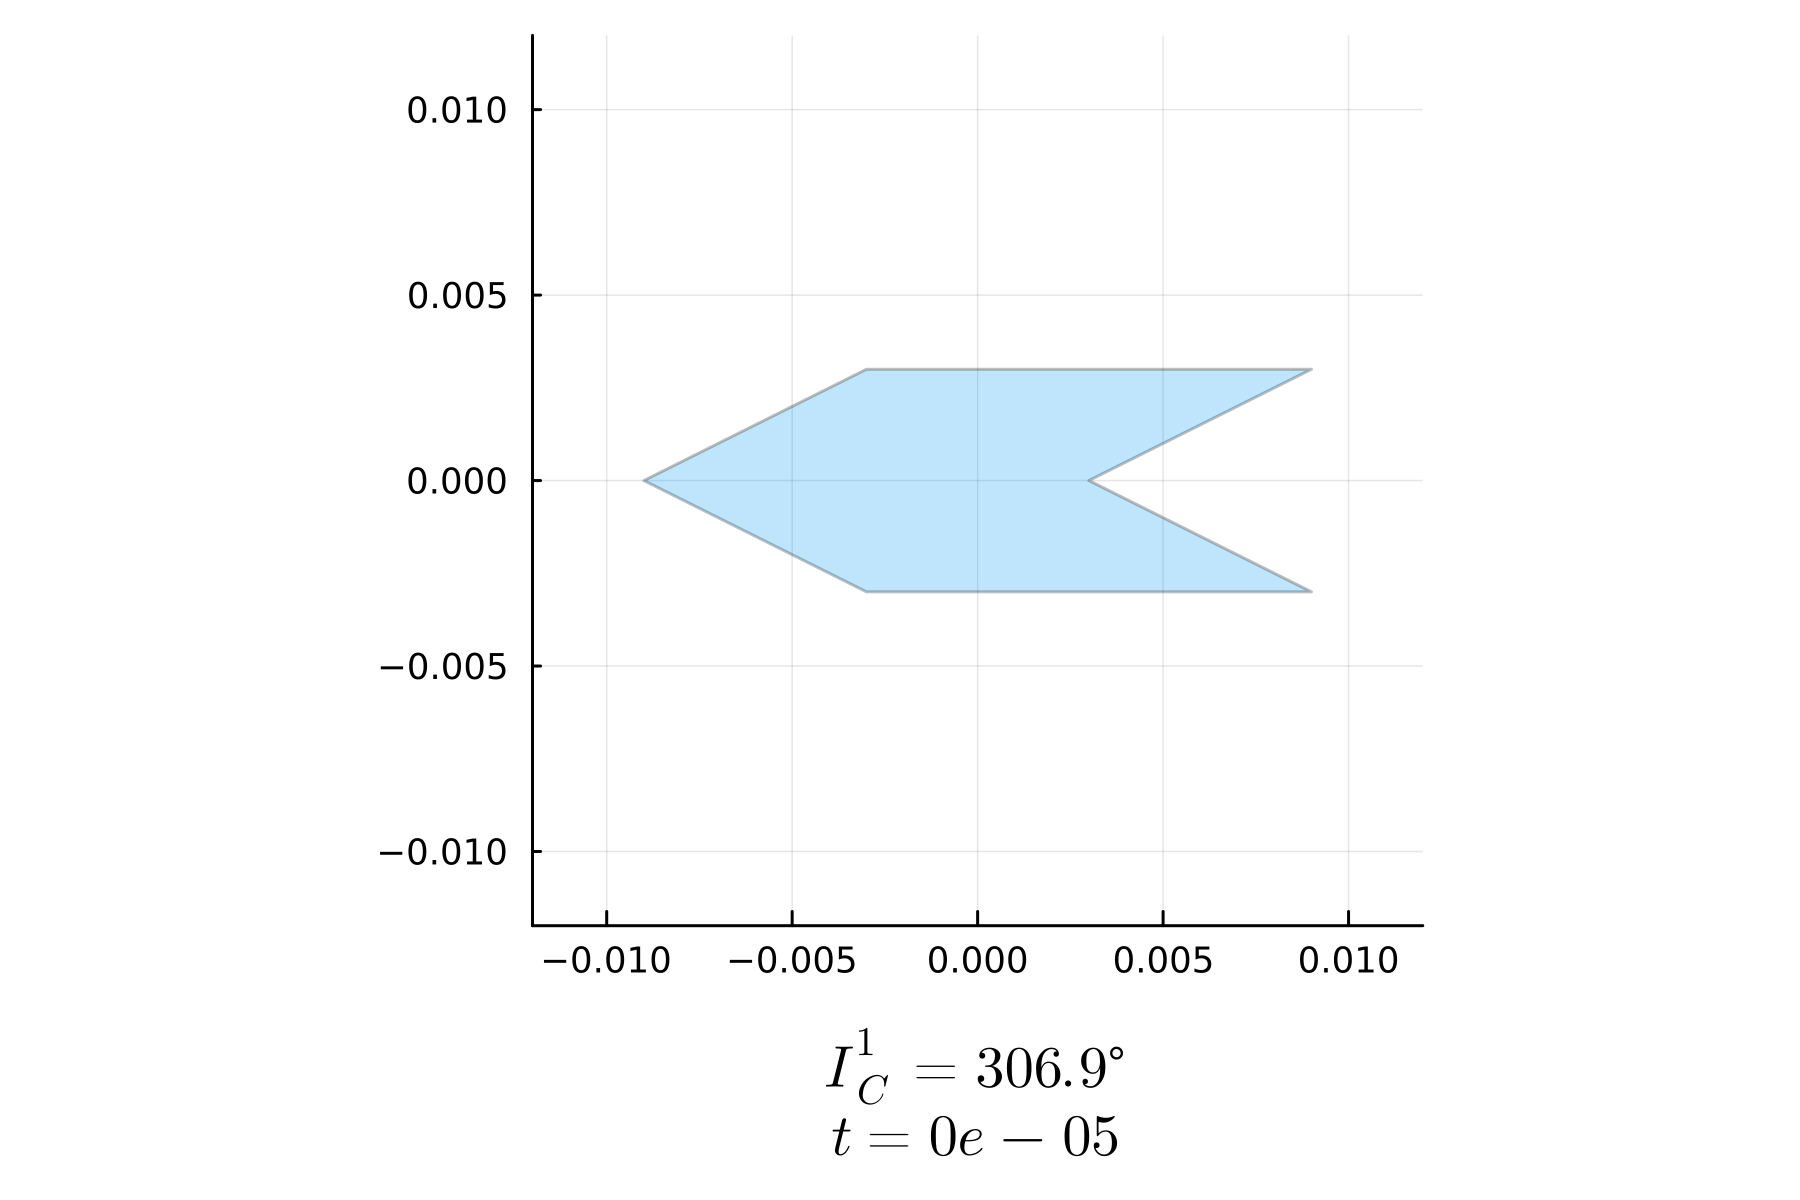
\includegraphics[width=0.5\textwidth]{forces/angle1/t0.png} &
        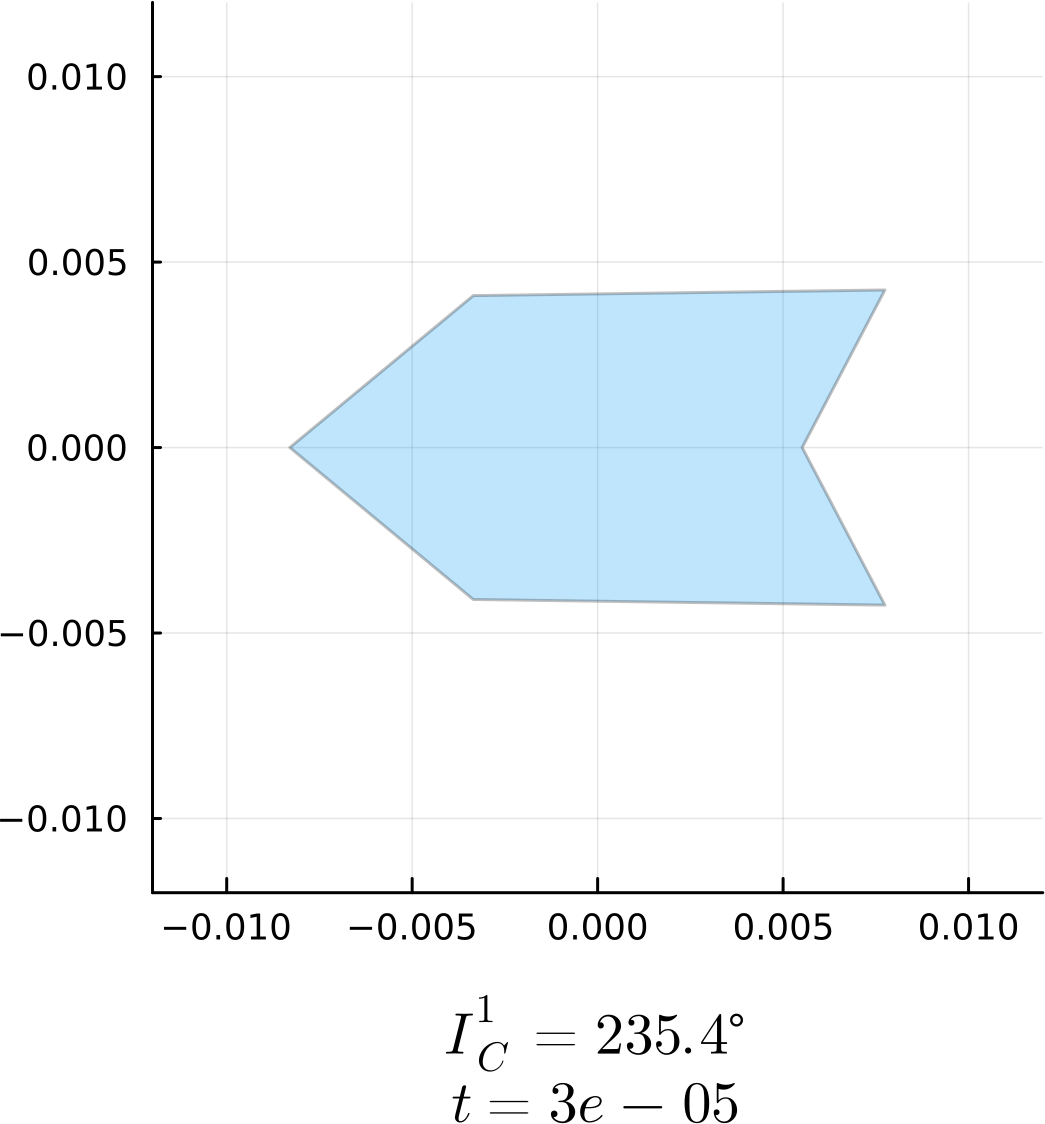
\includegraphics[width=0.5\textwidth]{forces/angle1/t3.png} \\
        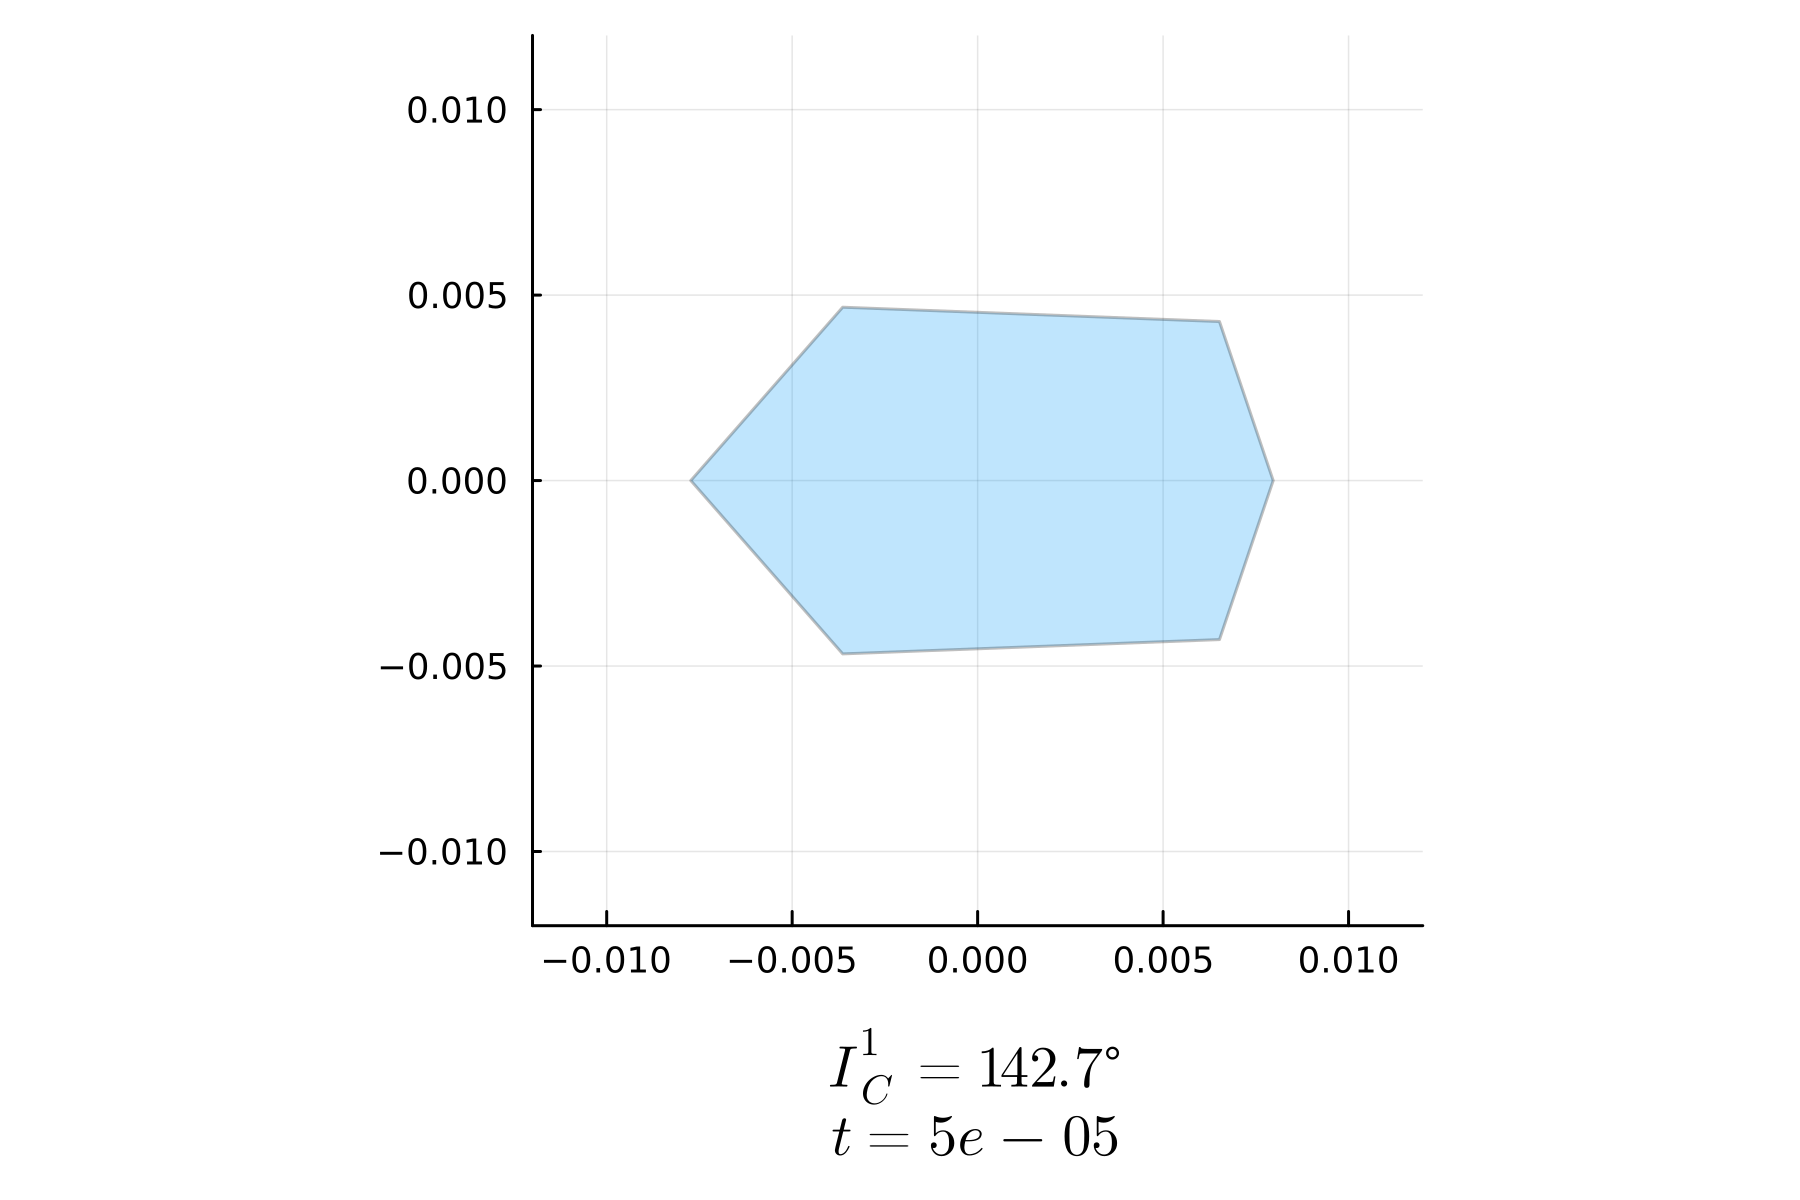
\includegraphics[width=0.5\textwidth]{forces/angle1/t5.png} &
        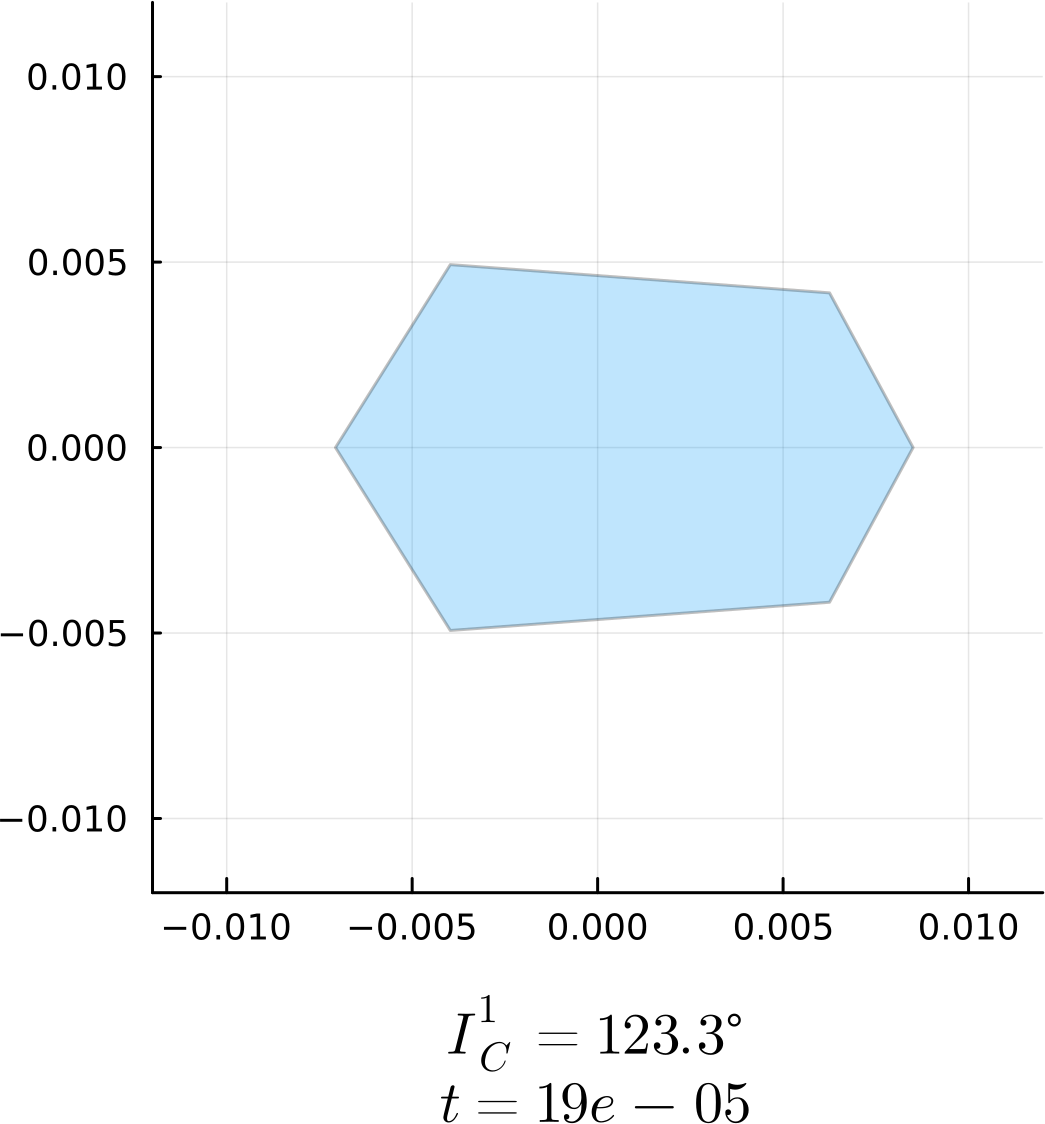
\includegraphics[width=0.5\textwidth]{forces/angle1/t19.png} \\
    \end{tabular}
    \caption{The top four plots depict the evolution of a DF cell subject only to the interior angle force with $k=2$ applied to the vertices and a force scaling of $1\times 10^{-1}$, at times $t \in \{0, 3\times 10^{-5}, 5\times 10^{-5}, 19\times 10^{-5}\}$.\\
			In this case, we have $\frac{\dequ \vec{v}}{\dequ t} = - 1\times 10^{-1} \nabla_{\vec{v}} I_2(C)$ for all vertices.\\
			At the vertex with initial position $\vec{v}_1 = (0.003, 0.0)^T$, the starting interior angle is $306.9°$, while all desired interior angles are $120°$.\\
			Click \href{https://github.com/tivo476c/FlexibleCellModel/blob/master/figures/gifs/showForces/show-intAngleForce.gif}{\textit{here}} to view the corresponding animation (GIF).\\
			As seen in Figure~\ref{fig:angleEnergyDiagram}, the interior angle force requires more time to reach the target configuration. 
			This slower convergence is due to the reduced force scaling, which was necessary to avoid stability issues encountered at higher force scaling values. }
	\label{fig:angleForce}
\end{figure}
\begin{figure}[h!]
    \centering
        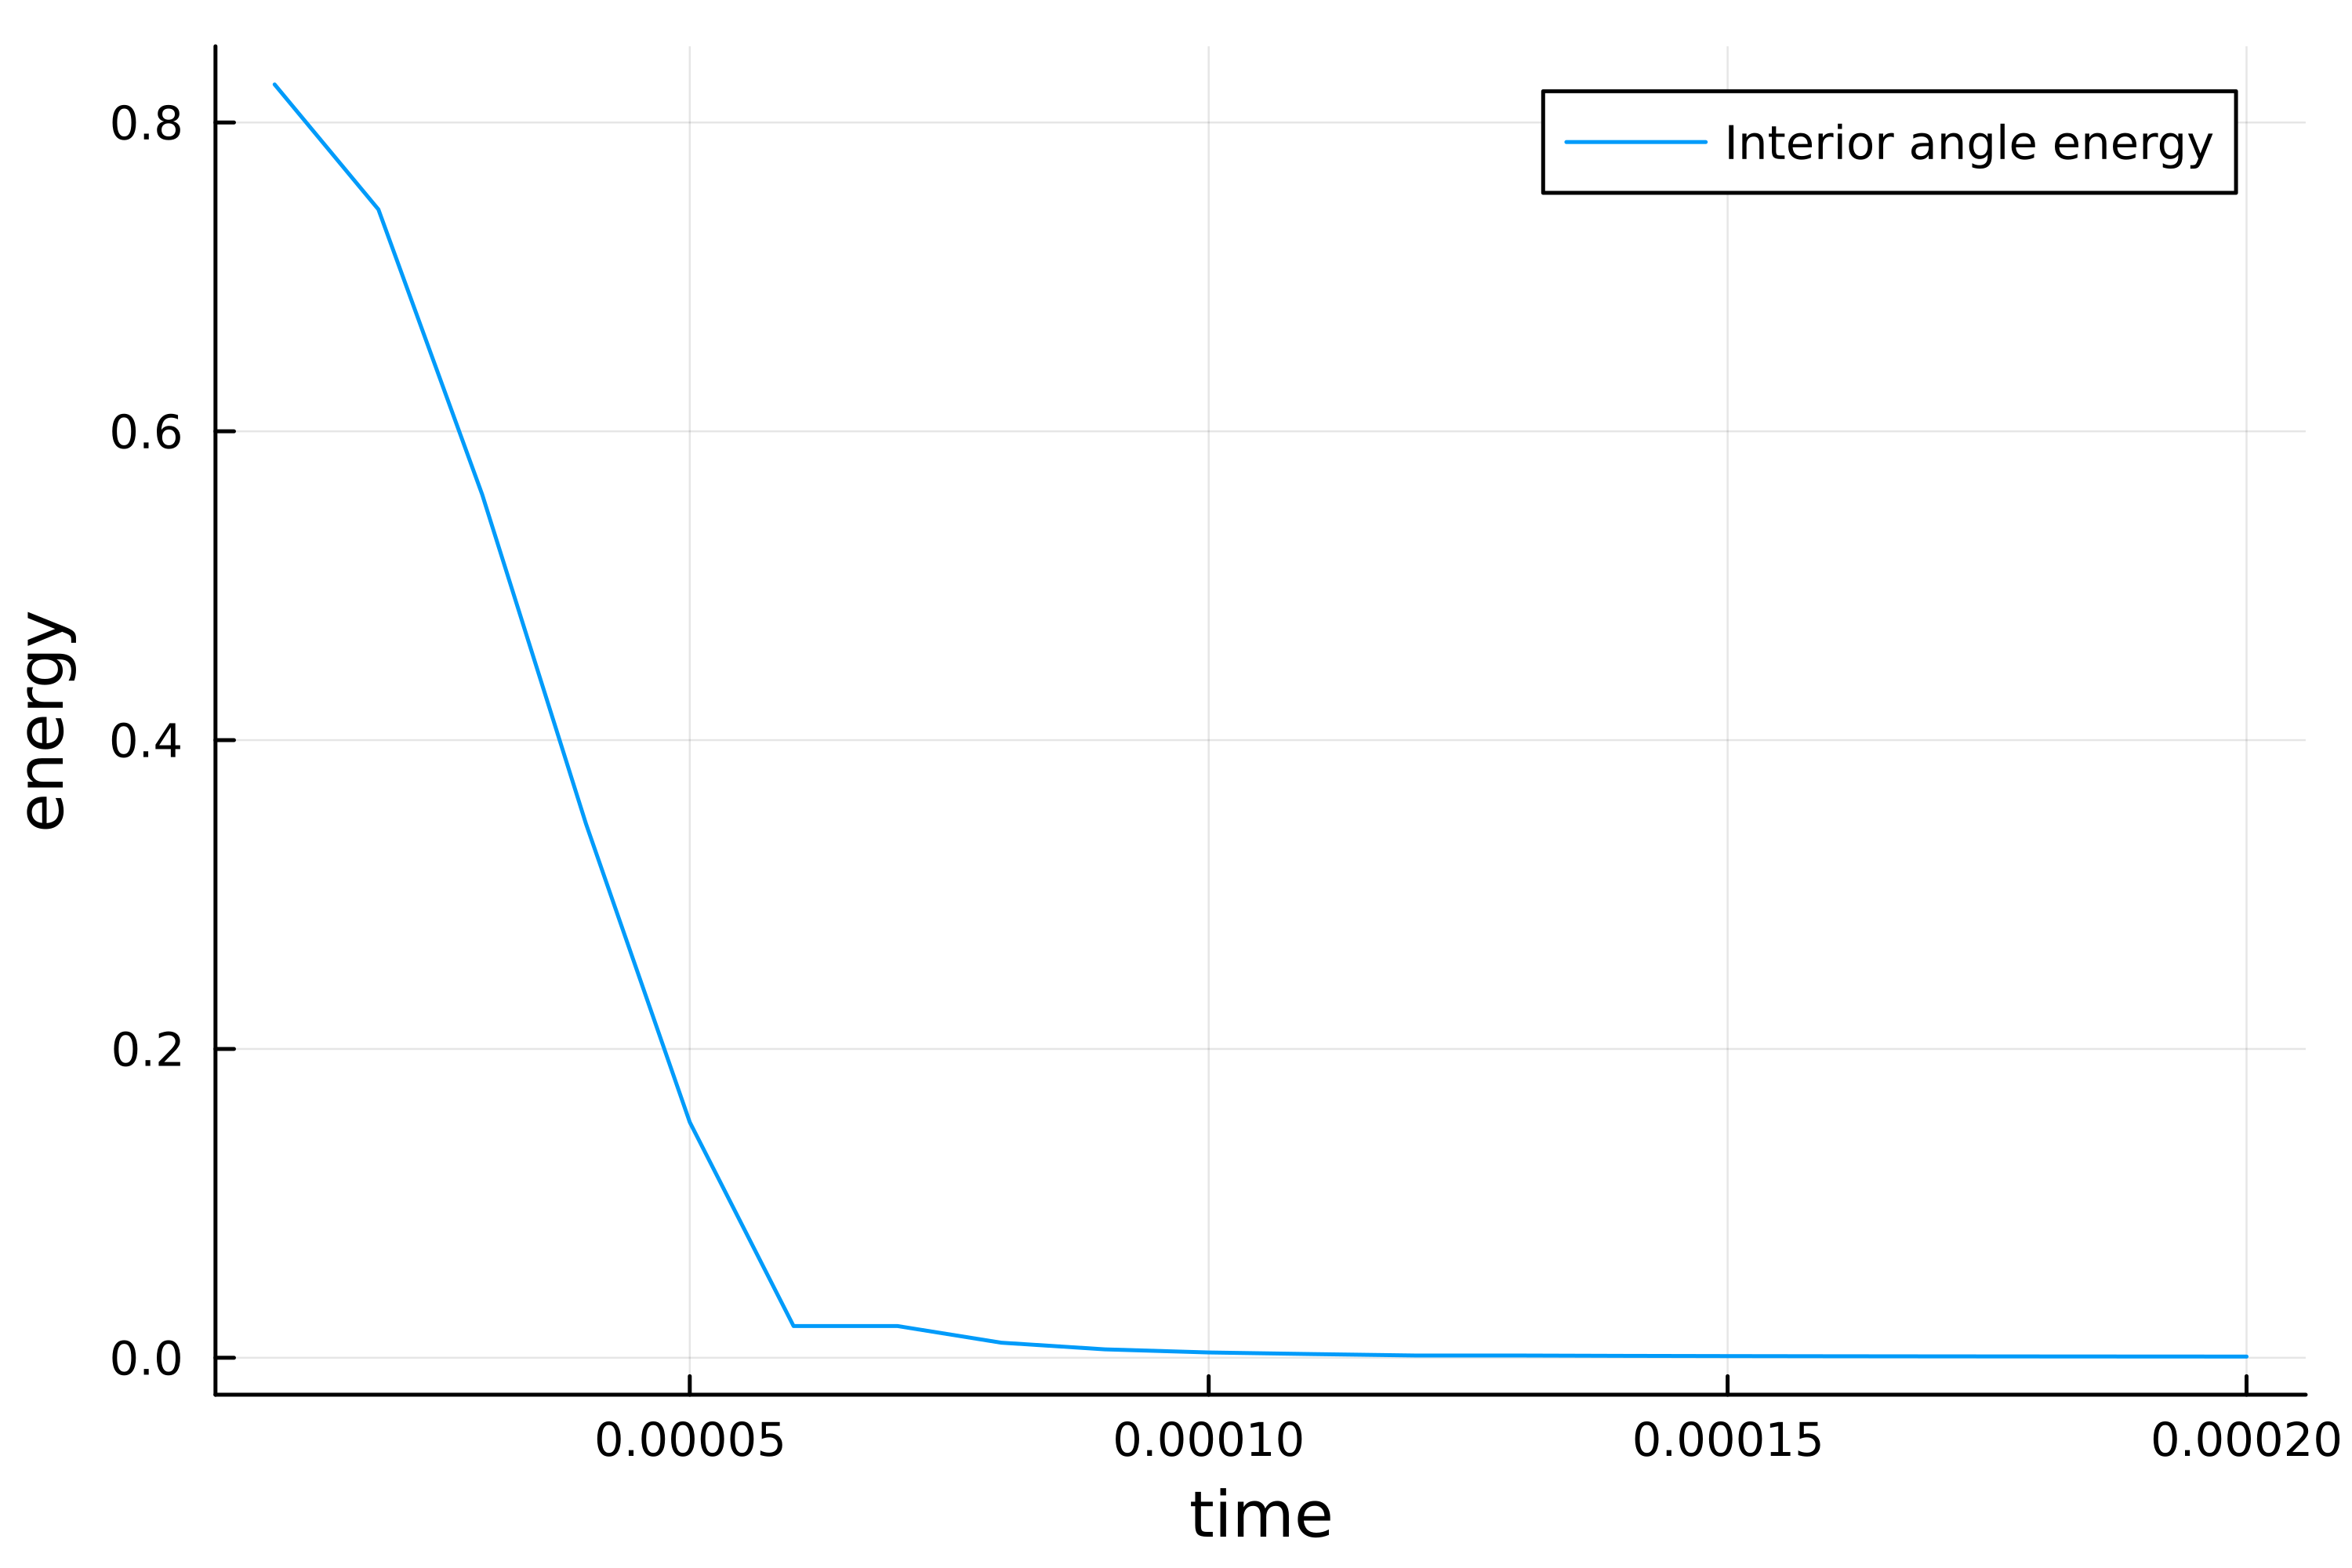
\includegraphics[width=0.7\textwidth]{forces/angle1/energies-show-intAngleForce.png} 
    \caption{The interior angle force is able to minimize the interior angle energy over time.}
	\label{fig:angleEnergyDiagram}    
\end{figure}

\subsection{Overlap force}
% explain the algorithm
Unlike the previous energies, which act independently on each cell, the overlap force is the first to account for interactions between multiple cells, thereby introducing cell-to-cell interaction into the simulation. \\

\subsubsection*{Deforming overlap force}
The first overlap force, that we want to introduce, is an adapted form of the overlap force introduced in~\cite{Vogel2023}. 
It degenerates a cell overlap by influencing that cell shapes of the affected cells. \\
The challenging aspect of computing the overlap force lies in detecting overlaps within the cell system. 
\begin{definition} \textbf{Overlap cell}\\
	An overlap cell between two DF cells $C_i$ and $C_m$ is a DF cell in the sence of Definition~\ref{def:DF}, composed of all vertices of $C_i$ that lie inside $C_m$, all vertices of $C_m$ that lie inside $C_i$ and the intersection points of the cell walls of $C_i$ and $C_m$.
\end{definition}
Each pair of cells can have more than one overlap cell in unfavourable configurations.
To be able to catch the correct dynamic in all cases, we need to introduce the set of all overlaps between a pair of DF cells.
\begin{definition} \textbf{Set of overlaps $\Omega_{C_i,C_m}$}\\
	Let $C_i, C_m \in \vec{C}$ be two DF cells. 
	Then, the set of overlaps $\Omega_{C_i,C_m}$ is defined as
	\[
		\Omega_{C_i,C_m} = \{\, D \mid D \text{ is an overlap cell formed between } C_i \text{ and } C_m \,\}.
	\]
\end{definition}
%TODO: add an example figure with 2 DF cells having two overlaps and write down what Omega_1,2 is and what their overlaps are
Once all overlaps have been identified, we apply a dynamic similar to that of the area force, but with a desired area of zero. 
This generates a force that acts to eliminate the overlap by reducing its area to zero. 
The resulting force is then applied to the vertices of the original cells that define the overlapping region. \\
The first step in detecting overlaps is identifying the intersection points between cell boundaries.
Intersections can be identified by representing the cell edges as line segments and computing the intersection points between segments belonging to different cells. \\
Having found all intersections, we can apply the following algorithm, that can be used to compute all overlaps between two cells. 

\begin{algorithm} \textbf{Computation of a discrete overlap} \label{alge:discreteOverlap}
	\begin{itemize} 
		\itemsep0em 
		\item[] \text{INPUT:}
		\item Discrete cells  $C$and $\zeta$
		\item List $I$ of unused intersections of $C$ and $\zeta$ 
	\end{itemize}
	\begin{algorithmic}
		\Function{constructOverlap}{$C$, $\zeta$, $I$}		
			\State usedIntersections = List$\{$Intersection$\}$(I[1]) 
			\State newOverlap = List$\{$Vertices$\}$(I[1]) 
			\State currentIntersection = I[1]
			
			\For{counter = 1 : length(I)} 
			
				\If{counter is even}
					\State newPath, newIntersection = findPath(currentIntersection, $C$, $I$) 
				\Else 
					\State newPath, newIntersection = findPath(currentIntersection, $\zeta$, $I$) 
				\EndIf
				
				\State append!(newOverlap, newPath)
				\If{newIntersection == I[1]} 
					\State \Return newOverlap, usedIntersections
				\Else 
					\State append!(newOverlap, newIntersection)
					\State append!(usedIntersections, newIntersection) 
					\State currentIntersection = newIntersection
				\EndIf
			\EndFor
		\EndFunction
	\end{algorithmic}
	\begin{itemize} 
		\itemsep0em 
		\item[] \text{OUTPUT:}
		\item A single intersection `newOverlap' which occurs between $C$ and $\zeta$ and which uses vertices from  $C$ and $\zeta$ as well as only intersections from $I$
		\item A list `usedIntersections' of all intersection that are used in `newOverlap'
	\end{itemize}	
\end{algorithm}
%TODO; rewrite that shit 
The algorithm begins by selecting the first intersection point $I[1]$ from the list $I$ as the initial vertex of the overlap cell `newOverlap'. 
This point is also added to the list `usedIntersections' \\
Next, the function `getOverlap' calls another function, `findPath', which determines the path along the discrete cell $\zeta$ from the current intersection point to the next intersection in $I$ encountered while traversing the edges of $\zeta$. 
This next intersection is also returned by the function. 
The identified path is a list of vertices in $\zeta$ that lie strictly between the two intersections. 
It may be empty if the next intersection occurs on the same edge as the current one. 
Both the path and the newly found intersection are appended to `newOverlap', and the intersection is also added to the list usedIntersections.\\
Since each intersection implies changing the cell from which the overlapping cell uses the edges, `findPath' is now applied to the other cell. 
Again, it will deliver the next intersection as well as a list of the in between laying vertices. 
The vertex list always gets appended to `newOverlap'. \\
If the newly found intersection is equal to the initial intersection $I[1]$, then the construction of the discrete overlap cell `newOverlap' is complete. 
At this point, both `newOverlap' and `usedIntersections' can be returned by the function `constructOverlap'. \\
Otherwise, the newly found intersection is appended to both `newOverlap' and `usedIntersections', and the process continues by calling `findPath' on the other discrete cell.   
This step is repeated until the starting intersection is reached, completing the overlap cell construction. \\
Once an overlap between $C$ and $\zeta$ has been successfully extracted, all intersections used in its construction can be removed from the list $I$, since each intersection point belongs to exactly one overlap. 
As long as $I$ is not empty, the function `constructOverlap' can be called again with the updated list to extract the next overlap. 
When $I$ is empty, we can be certain that all intersections between $C$ and $\zeta$ have been processed, and thus all overlaps between the two cells have been identified. \\

Each time `findPath' is called, it is not immediately clear in which direction the function should traverse the vertices of the given cell. 
However, the correct direction can be determined using the following approach. \\
Starting from the current intersection passed into the function, move a small distance in one direction along the edge of the given cell where the intersection is located. Next, check whether this new point lies within the boundaries of the other cell as well. 
If the point is found in both cells, the chosen direction is correct. 
If not, then the opposite direction must be used. \\ 
A simple method to determine whether a point lies inside a polygon is to draw a ray from the point to the outside of the polygon. 
The number of intersections between the ray and the polygon's edges determines the point's position. 
If the number of intersections is odd, the point is inside the polygon.
If it is even, the point is outside the polygon. \\ 
\smallskip  \\
% until here the rewriting!! 
% then continue with the energy and the force 
After introducing the method for detecting overlaps, we can now define the overlap force, which acts on the cell vertices involved in an overlap. 
This force is first computed based on the geometry of the overlap and then distributed to the corresponding vertices of the original cells. 

\begin{definition} \textbf{Overlap energy} \\
	Let $C_i$ and $C_m$ be two cells from the system $\vec{C}$ and $\Omega_{C_i,C_m}$ be the set of all overlaps that appear between $C_i$ and $C_m$, like explained above. Then, the total overlap energy $O_k : (\R^{2N_V})^{N_C} \rightarrow \R$ of the cell system is given by the formula 
	\begin{align}
		O_k(\vec{C}) = \sum\limits_{i=1}^{N_C} \left( \sum\limits_{m=i+1}^{N_C} \left(\sum\limits_{D \in \Omega_{C_i,C_m}} \frac{1}{k}|A_{D}|^k\right) \right),		
	\end{align} 
	where $A_{D}$ is the area of the overlap $D$.  \\
	We define the inner bracket to be the overlap energy of the cell pair $C_i$ and $C_m$
	\begin{center}
		$O_k^{i,m}: (\R^{2 N_V})^2 \rightarrow \R$ \\[0.5em]
		$O_k^{i,m}(C_i, C_m) = \sum\limits_{D \in \Omega_{C_i,C_m}} \frac{1}{k}|A_{D}|^k.$
	\end{center} 
\end{definition}

To decrease the overlap areas during the simulation, we evaluate the gradient flow of the area energy with a desired area of zero which indicates the direction of motion for each vertex for reducing the overlap areas.

\newcommand{\vargs}{\ensuremath{\vec{v}_{\text{out}}^{\: i}, \vec{v}_{\text{in}}^{\: i}, \vec{v}_{\text{out}}^{\: m}, \vec{v}_{\text{in}}^{\: m}}}
\newcommand{\tu}{\ensuremath{(\vec{v}_{\text{out}}^{\: m} - \vec{v}_{\text{out}}^{\: i}) \times (\vec{v}_{\text{in}}^{\: m} - \vec{v}_{\text{out}}^{\: m})}}
\newcommand{\tl}{\ensuremath{(\vec{v}_{\text{in}}^{\: i} - \vec{v}_{\text{out}}^{\: i}) \times (\vec{v}_{\text{in}}^{\: m} - \vec{v}_{\text{out}}^{\: m})}}
\newcommand{\tz}{\ensuremath{\dfrac{\tu}{\tl}}}
\newcommand{\w}{\ensuremath{\vec{v}_{\text{out}}^{\: i} + \tz (\vec{v}_{\text{in}}^{\: i} - \vec{v}_{\text{out}}^{\: i})}}

\begin{definition} \textbf{Intersection point and adjacent vertices} \\
	The vertices of an overlap cell $D$ can be divided into the vertices that are either in $C_i$ in $C_m$, we call that set 
	\[V(D) = \{\vec{v} \in D \:| \vec{v} \in C_i \cup C_m \}, \] 
	and into the vertices that are neither in $C_i$ nor $C_m$, named 
	\[W(D) = D \setminus V(D).\]
	All overlap vertices in $W(D)$ are intersections between the cells $C_i$ and $C_m$. \\
	Each intersection $\vec{w}$ is dependent on two vertices of each cell that limit the edges that intersect, where the intersection point $\vec{w}$ arises. \\
	We call those four vertices \textbf{adjacent} to the intersection $\vec{w}$. 
	All intersection adjacent vertices will get an extra deforming overlap dynamic applied, since they influence the overlap area, and thus the overlap energy, via the intersection point they create. \\
	From each cell we get one vertex that is part of the overlap cell, called the inside vertex, and one vertex that is not part of the overlap, called the outside vertex. 
	For each intersection $\vec{w} \in W(D)$, we call its adjacent vertices 
	\[\text{adj}(\vec{w}) = \{\vec{v}_{\text{in}}^{\: i}, \vec{v}_{\text{out}}^{\: i}, \vec{v}_{\text{in}}^{\: m}, \vec{v}_{\text{out}}^{\: m} \}. \]
	In order to refer to the inside or outside vertices, we define the sets 
	\[ \text{in}(\vec{w}) = \{\vec{v}_{\text{in}}^{\: i}, \vec{v}_{\text{in}}^{\: m} \} \text{ and } \text{out}(\vec{w}) = \{\vec{v}_{\text{out}}^{\: i}, \vec{v}_{\text{out}}^{\: m} \}.\]
	Figure~\ref{fig:adjacent} illustrates what the in- and outside vertices of an intersection are. \\
	Given the four adjacent vertices, we can always compute the intersection with the function:
	\begin{center}
		$w: (\R^2)^4 \rightarrow \R^2$, \\[0.5em]
		$w(\vargs) = \vec{v}_{\text{out}}^{\: i} + \dfrac{(\vec{v}_{\text{out}}^{\: m} - \vec{v}_{\text{out}}^{\: i}) \times (\vec{v}_{\text{in}}^{\: m} - \vec{v}_{\text{out}}^{\: m})}{(\vec{v}_{\text{in}}^{\: i} - \vec{v}_{\text{out}}^{\: i}) \times (\vec{v}_{\text{in}}^{\: m} - \vec{v}_{\text{out}}^{\: m})} (\vec{v}_{\text{in}}^{\: i} - \vec{v}_{\text{out}}^{\: i})$,
	\end{center}
	where $(a^x, a^y)^T \times (b^x, b^y)^T = a^x b^y - a^y b^x$ denotes the two dimensional cross product. \\
\end{definition}

\begin{figure}
	\begin{center}
		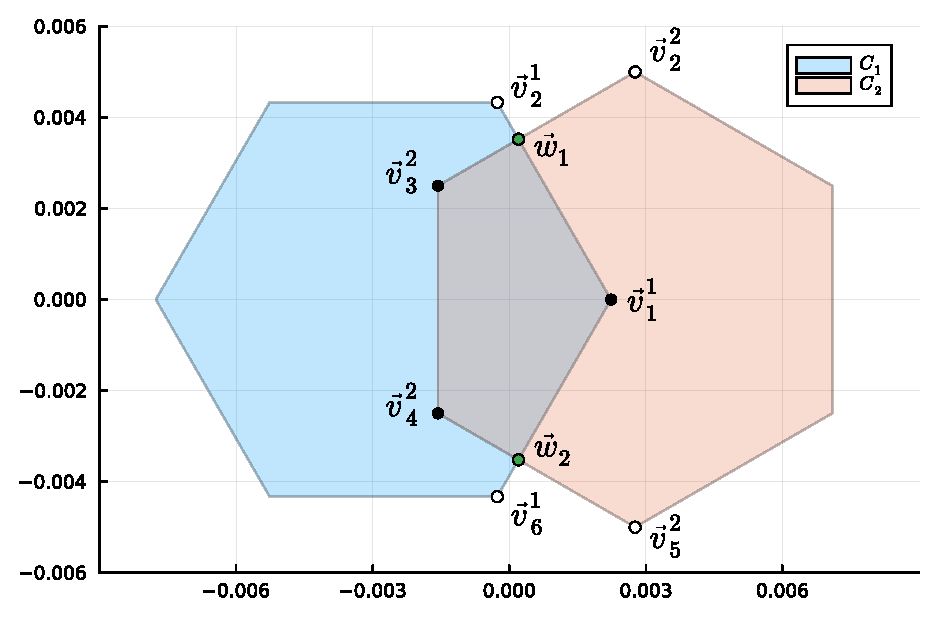
\includegraphics[width=14cm]{forces/adjacentVertices.pdf}
		\caption{
			Here, we can see a DF cell setup with two cells having an overlap. 
			The intersection points $\vec{w}_1$ and $\vec{w}_2$ are marked green. 
			We can also see all inside vertices colored in black and the outside vertices colored in white.
			In this example, we have $\text{adj}(\vec{w}_1) = \{\vec{v}_1^{\:1}, \vec{v}_2^{\:1}, \vec{v}_2^{\:2}, \vec{v}_3^{\:2}\}$, $\text{in}(\vec{w}_1) = \{\vec{v}_1^{\:1}, \vec{v}_3^{\:2}\}$ and $\text{out}(\vec{w}_1) = \{\vec{v}_2^{\:1}, \vec{v}_2^{\:2}\}$ for the first intersection and $\text{adj}(\vec{w}_2) = \{\vec{v}_1^{\:1}, \vec{v}_6^{\:1}, \vec{v}_4^{\:2}, \vec{v}_5^{\:2}\}$, $\text{in}(\vec{w}_2) = \{\vec{v}_1^{\:1}, \vec{v}_4^{\:2}\}$ and $\text{out}(\vec{w}_2) = \{\vec{v}_6^{\:1}, \vec{v}_5^{\: 2}\}$ for the second intersection.
			}
		\label{fig:adjacent}
	\end{center}
\end{figure}


\begin{proposition} \textbf{Partial derivatives of intersection points} \\
	We use $w(\vargs)$ to compute the influence of the adjacent vertices to the intersection point via their partial derivatives.
	In this proposition, we compute the needed partial derivatives. \\
	We define the following auxiliary terms:
	\begin{align*}
		f &= \tu \\[1em]
		g &= \tl\\[1em]
		t &= \frac{f}{g} \\[1em]
		w &= \vec{v}_{\text{out}}^{\: i} + t(\vec{v}_{\text{in}}^{\: i} - \vec{v}_{\text{out}}^{\: i}) \\[1em]
	\end{align*}
	It is sufficient to just compute the partial derivatives with respect to $\vec{v}_{\text{in}}^{\: i}$ and $\vec{v}_{\text{out}}^{\: i}$.
	If we want the dynamic for the vertices of the other cell, we just switch the arrangement of the arguments (switch $\vec{v}_{\text{in}}^{\: i}$ with $\vec{v}_{\text{in}}^{\: j}$ and $\vec{v}_{\text{out}}^{\: i}$ with $\vec{v}_{\text{out}}^{\: j}$) and then use the same partial derivatives as for the first cell. \\
	The partial derivatives are: 
	\begin{align}
		\begin{split}
			D_{\vec{v}_{\text{out}}^{\: i}} w(\vargs): (\R^2)^4 \rightarrow \R^{2 \times 2}, \\[0.5em]
			D_{\vec{v}_{\text{out}}^{\: i}} w(\vargs) = (1-t)I_2 + \dfrac{g - f}{g^2}(\vec{v}_{\text{in}}^{\: i} - &\vec{v}_{\text{out}}^{\: i}) \begin{pmatrix}
			-(v_{\text{in}}^{m, y} - v_{\text{out}}^{m, y}) \\[0.5em]
			 v_{\text{in}}^{m, x} - v_{\text{out}}^{m, x}
		\end{pmatrix}^T,
		\end{split}
		\label{equ:dwv_out}
	\end{align}

	\begin{align}
		\begin{split}
			D_{\vec{v}_{\text{in}}^{\: i}} w(\vargs): (\R^2)^4 \rightarrow \R^{2 \times 2}, \\[0.5em]
			D_{\vec{v}_{\text{in}}^{\: i}} w(\vargs) = t I_2 \:+\: \dfrac{f}{g^2}(\vec{v}_{\text{in}}^{\: i} \;-\; &\vec{v}_{\text{out}}^{\: i}) \begin{pmatrix}
			-(v_{\text{in}}^{m, y} - v_{\text{out}}^{m, y}) \\[0.5em]
			 v_{\text{in}}^{m, x} - v_{\text{out}}^{m, x}
		\end{pmatrix}^T.
		\end{split}
		\label{equ:dwv_in}
	\end{align}

	Proof.\\

	First of all, we compute the gradients of $f$ and $g$: 
	\begin{align*}
		\nabla_{\vec{v}_{\text{out}}^{\: i}} f 
		&= \nabla_{\vec{v}_{\text{out}}^{\: i}}[(v_{\text{out}}^{m, x} - v_{\text{out}}^{i, x})(v_{\text{in}}^{m, y} - v_{\text{out}}^{m, y}) - (v_{\text{out}}^{m, y} - v_{\text{out}}^{i, y})(v_{\text{in}}^{m, x} - v_{\text{out}}^{m, x})] \\[0.5em]
		&= \begin{pmatrix}
			-(v_{\text{in}}^{m, y} - v_{\text{out}}^{m, y}) \\[0.5em]
			 v_{\text{in}}^{m, x} - v_{\text{out}}^{m, x}
		\end{pmatrix}, 
	\end{align*}

	\begin{align*}
		\nabla_{\vec{v}_{\text{in}}^{\: i}} f 
		&= \nabla_{\vec{v}_{\text{in}}^{\: i}}[(v_{\text{out}}^{m, x} - v_{\text{out}}^{i, x})(v_{\text{in}}^{m, y} - v_{\text{out}}^{m, y}) - (v_{\text{out}}^{m, y} - v_{\text{out}}^{i, y})(v_{\text{in}}^{m, x} - v_{\text{out}}^{m, x})] \\[0.5em]
		&= \begin{pmatrix}
			0 \\
			0
		\end{pmatrix}, 
	\end{align*}

	\begin{align*}
		\nabla_{\vec{v}_{\text{out}}^{\: i}} g
		&= \nabla_{\vec{v}_{\text{out}}^{\: i}}[(v_{\text{in}}^{i, x} - v_{\text{out}}^{i, x})(v_{\text{in}}^{m, y} - v_{\text{out}}^{m, y}) - (v_{\text{in}}^{i, y} - v_{\text{out}}^{i, y})(v_{\text{in}}^{m, x} - v_{\text{out}}^{m, x})] \\[0.5em]
		&= \begin{pmatrix}
			-(v_{\text{in}}^{m, y} - v_{\text{out}}^{m, y}) \\[0.5em]
			 v_{\text{in}}^{m, x} - v_{\text{out}}^{m, x}
		\end{pmatrix}, 
	\end{align*}

	\begin{align*}
		\nabla_{\vec{v}_{\text{in}}^{\: i}} g
		&= \nabla_{\vec{v}_{\text{in}}^{\: i}}[(v_{\text{in}}^{i, x} - v_{\text{out}}^{i, x})(v_{\text{in}}^{m, y} - v_{\text{out}}^{m, y}) - (v_{\text{in}}^{i, y} - v_{\text{out}}^{i, y})(v_{\text{in}}^{m, x} - v_{\text{out}}^{m, x})] \\[0.5em]
		&= \begin{pmatrix}
			v_{\text{in}}^{m, y} - v_{\text{out}}^{m, y} \\[0.5em]
			-(v_{\text{in}}^{m, x} - v_{\text{out}}^{m, x})
		\end{pmatrix}. \\[2em]
	\end{align*}
	Now, we can succeed with the gradients of $t$:
	\begin{align*}
		\nabla_{\vec{v}_{\text{out}}^{\: i}} t
		&= \nabla_{\vec{v}_{\text{out}}^{\: i}} \dfrac{f}{g} \\
		&= \dfrac{(\nabla_{\vec{v}_{\text{out}}^{\: i}} f) g - (\nabla_{\vec{v}_{\text{out}}^{\: i}} g) f}{g^2} \\[0.5em]
		&= \dfrac{1}{g^2} \left(\begin{pmatrix}
			-(v_{\text{in}}^{m, y} - v_{\text{out}}^{m, y}) \\[0.5em]
			 v_{\text{in}}^{m, x} - v_{\text{out}}^{m, x}
		\end{pmatrix} g - \begin{pmatrix}
			-(v_{\text{in}}^{m, y} - v_{\text{out}}^{m, y}) \\[0.5em]
			 v_{\text{in}}^{m, x} - v_{\text{out}}^{m, x}
		\end{pmatrix} f\right)\\[0.5em]
		&= \dfrac{g - f}{g^2} \begin{pmatrix}
			-(v_{\text{in}}^{m, y} - v_{\text{out}}^{m, y}) \\[0.5em]
			 v_{\text{in}}^{m, x} - v_{\text{out}}^{m, x}
		\end{pmatrix}\\[1em]
	\end{align*}
	\begin{align*}	
		\nabla_{\vec{v}_{\text{in}}^{\: i}} t
		&= \nabla_{\vec{v}_{\text{in}}^{\: i}} \dfrac{f}{g} \\
		&= \dfrac{(\nabla_{\vec{v}_{\text{in}}^{\: i}} f) g - (\nabla_{\vec{v}_{\text{in}}^{\: i}} g) f}{g^2} \\[0.5em]
		&= \dfrac{1}{g^2} \left( - \begin{pmatrix}
			v_{\text{in}}^{m, y} - v_{\text{out}}^{m, y} \\[0.5em]
			-(v_{\text{in}}^{m, x} - v_{\text{out}}^{m, x})
		\end{pmatrix} f\right). \\[0.5em]
		&= \dfrac{f}{g^2} \begin{pmatrix}
			-(v_{\text{in}}^{m, y} - v_{\text{out}}^{m, y}) \\[0.5em]
			v_{\text{in}}^{m, x} - v_{\text{out}}^{m, x}
		\end{pmatrix}. \\[0.5em]
	\end{align*}

	And finally, we can compute the partial derivatives of $w = (w_1, w_2)^T$:
	\begin{align*}
		\dfrac{\partial w_1}{\partial v_{\text{out}}^{i, x}} = 1 + \dfrac{\partial t}{\partial v_{\text{out}}^{i, x}}(v_{\text{in}}^{i, x}- v_{\text{out}}^{i, x}) - t, &\quad 
		\dfrac{\partial w_1}{\partial v_{\text{out}}^{i, y}} = 0 + \dfrac{\partial t}{\partial v_{\text{out}}^{i, y}}(v_{\text{in}}^{i, x}- v_{\text{out}}^{i, x}) + 0, \\[0.5em]
		\dfrac{\partial w_2}{\partial v_{\text{out}}^{i, x}} = 0 + \dfrac{\partial t}{\partial v_{\text{out}}^{i, x}}(v_{\text{in}}^{i, y}- v_{\text{out}}^{i, y}) + 0, &\quad 
		\dfrac{\partial w_2}{\partial v_{\text{out}}^{i, y}} = 1 + \dfrac{\partial t}{\partial v_{\text{out}}^{i, y}}(v_{\text{in}}^{i, y}- v_{\text{out}}^{i, y}) - t, \\[0.5em]
		\Rightarrow D_{\vec{v}_{\text{out}}^{\: i}} w = (1-t)I_2 + (\vec{v}_{\text{in}}^{\: i} - \vec{v}_{\text{out}}^{\: i}) &(\nabla_{\vec{v}_{\text{out}}^{\: i}} t)^T \\[0.5em]
		= (1-t)I_2 + (\vec{v}_{\text{in}}^{\: i} - \vec{v}_{\text{out}}^{\: i}) &\left(\dfrac{g - f}{g^2} \begin{pmatrix}
			-(v_{\text{in}}^{m, y} - v_{\text{out}}^{m, y}) \\[0.5em]
			 v_{\text{in}}^{m, x} - v_{\text{out}}^{m, x}
		\end{pmatrix}\right)^T \\[0.5em]
		= (1-t)I_2 + \dfrac{g - f}{g^2}(\vec{v}_{\text{in}}^{\: i} - &\vec{v}_{\text{out}}^{\: i}) \begin{pmatrix}
			-(v_{\text{in}}^{m, y} - v_{\text{out}}^{m, y}) \\[0.5em]
			 v_{\text{in}}^{m, x} - v_{\text{out}}^{m, x}
		\end{pmatrix}^T, \\[0.5em]
	\end{align*}
	
	\begin{align*}
		\dfrac{\partial w_1}{\partial v_{\text{in}}^{i, x}} = \dfrac{\partial t}{\partial v_{\text{in}}^{i, x}}(v_{\text{in}}^{i, x}- v_{\text{out}}^{i, x}) + t, &\quad 
		\dfrac{\partial w_1}{\partial v_{\text{in}}^{i, y}} = \dfrac{\partial t}{\partial v_{\text{in}}^{i, y}}(v_{\text{in}}^{i, x}- v_{\text{out}}^{i, x}) + 0, \\[0.5em]
		\dfrac{\partial w_2}{\partial v_{\text{in}}^{i, x}} = \dfrac{\partial t}{\partial v_{\text{in}}^{i, x}}(v_{\text{in}}^{i, y}- v_{\text{out}}^{i, y}) + 0, &\quad 
		\dfrac{\partial w_2}{\partial v_{\text{in}}^{i, y}} = \dfrac{\partial t}{\partial v_{\text{in}}^{i, y}}(v_{\text{in}}^{i, y}- v_{\text{out}}^{i, y}) + t, \\[0.5em]
	\end{align*}
	\begin{align*}
		\Rightarrow D_{\vec{v}_{\text{in}}^{\: i}} w = t I_2 + (\vec{v}_{\text{in}}^{\: i} - \vec{v}_{\text{out}}^{\: i}) &(\nabla_{\vec{v}_{\text{in}}^{\: i}} t)^T \\[0.5em]
		= t I_2 + (\vec{v}_{\text{in}}^{\: i} - \vec{v}_{\text{out}}^{\: i}) &\left(\dfrac{f}{g^2} \begin{pmatrix}
			-(v_{\text{in}}^{m, y} - v_{\text{out}}^{m, y}) \\[0.5em]
			v_{\text{in}}^{m, x} - v_{\text{out}}^{m, x}
		\end{pmatrix}\right)^T \\[0.5em]
		= \; t I_2 \:+\: \dfrac{f}{g^2}(\vec{v}_{\text{in}}^{\: i} \;-\; &\vec{v}_{\text{out}}^{\: i}) \begin{pmatrix}
			-(v_{\text{in}}^{m, y} - v_{\text{out}}^{m, y}) \\[0.5em]
			 v_{\text{in}}^{m, x} - v_{\text{out}}^{m, x}
		\end{pmatrix}^T. \\[0.5em]
	\end{align*}

	
\end{proposition}

\begin{proposition} \textbf{Deforming overlap force} \\
	Each overlap cell $D \in \Omega_{C_i,C_m}$ is a list of vertices, that form the overlap, just like a DF cell. \\
	The deforming overlap gradient is then given by 
	\begin{align}
		\begin{split}
			\nabla_{\vec{v}_j^{\: i}} O_k(\vec{C}) &= \sum\limits_{D \in \Omega_{C_i,C_m}}  |A_{D}|^{k-1} \Biggl(\mathbf{1}_{V(D)}(\vec{v}_j^{\: i}) \nabla_{\vec{v}_j^{\: i}}A(D)  + \\[0.5em]
				    							   &+ \sum\limits_{\vec{w} \in W(D)} \left(\mathbf{1}_{\text{out}(w)}(\vec{v}_{j}^{\: i}) D_{\vec{v}_{\text{out}}^{\: i}} \vec{w} %+ \\
													+ \mathbf{1}_{\text{in}(w)}(\vec{v}_j^{\: i}) D_{\vec{v}_{\text{in}}^{\: i}} \vec{w} \right) \nabla_{\vec{w}}A(D)\Biggr),
		\end{split}
	\end{align}
	for all $1 \leq j \leq N_V$ and $1 \leq i \leq N_C$, where $\text{out}(w)$, $\text{in}(w) \subset \text{adj}(w)$ denote the sets of outside and inside overlap-adjacent vertices, respectively. \\
	Note, that the Formulas \ref{equ:dwv_out} and \ref{equ:dwv_in} define $\frac{\partial \vec{w}}{\partial \vec{v}_{j, out}^{\: i}}$ and $\frac{\partial \vec{w}}{\partial \vec{v}_{j, in}^{\: i}}$, respectively. \\
	The difference between $\nabla_{\vec{v}_j^{\: i}}A(D)$ and $\nabla_{\vec{w}}A(D)$ is that $\nabla_{\vec{v}_j^{\: i}}A(D)$ uses the neighboring overlap vertices of $\vec{v}_j^{\: i}$ itself in the Area Gradient Formula \ref{gradient:area}, whereas $\nabla_{\vec{w}}A(D)$ uses the neighbors of the corresponding intersection point in $D$, which is not the same overlap vertex as $\vec{v}_j^{\: i}$.
    $A_{D}$ is the area of the overlap $D$.\\
	The indicator function $\mathbf{1}_{A}(\vec{v})$ equals one, if $\vec{v} \in A$ and is zero otherwise. \\
	The deforming overlap force $F_{k}^{\hat{(O)}}: (\R^{2 N_V})^{N_C} \rightarrow (\R^{2 N_V})^{N_C}$ that gets applied on the whole cell system $\vec{C} = (C_1, \ldots, C_{N_C})$ is then given by  
	\begin{align*}
		F_{k}^{\hat{(O)}}(\vec{C}) 
		= - (\nabla_{\vec{v}_1^{\:1}} O_k(\vec{C}), \ldots, \nabla_{\vec{v}_{N_V}^{\:1}} O_k(\vec{C}), \; \cdots \;, \vec{v}_1^{\:N_C} O_k(\vec{C}), \ldots, \nabla_{\vec{v}_{N_V}^{\:N_C}} O_k(\vec{C}))^T.
	\end{align*}
	For addressing the overlap force that acts on cell $1 \leq i \leq N_C$, we define 
	\begin{center}
		$F_{k, i}^{\hat{(O)}}: (\R^{2 N_V})^{N_C} \rightarrow (\R^{2 N_V})$, \\
		$F_{k, i}^{\hat{(O)}}(\vec{C}) = - (\nabla_{\vec{v}_1^{\:i}} O_k(\vec{C}), \ldots, \nabla_{\vec{v}_{N_V}^{\:i}} O_k(\vec{C}))^T$. 
	\end{center}

	Proof. \\
	%TODO: change from A_D^k to (A_D)^k
	Although we did not noted it like this before, we must be aware that $A_D$ is actually dependent on all overlap vertices, e.g. $A_D = A(D)$.
	We will also use that notation in the coming computation. 
	Since the area $A(D)$ is always positive, we can drop the absolute value. \\
	We aim to compute 
	\begin{align*}
		\nabla_{\vec{v}_j^{\: i}} O_k(\vec{C}) 
		&= \nabla_{\vec{v}_j^{\: i}} \sum\limits_{i=1}^{N_C} \left( \sum\limits_{m=i+1}^{N_C} \left(\sum\limits_{D \in \Omega_{C_i,C_m}} \frac{1}{k}A_{D}^k\right) \right) \\
		&= \nabla_{\vec{v}_j^{\: i}} \sum\limits_{m \neq i} O_k^{i,m}(C_i, C_m) \\
		&= \nabla_{\vec{v}_j^{\: i}} \sum\limits_{m \neq i} \sum\limits_{D \in \Omega_{C_i,C_m}} \frac{1}{k}A(D)^k \\
		&= \sum\limits_{m \neq i} \sum\limits_{D \in \Omega_{C_i,C_m}} \nabla_{\vec{v}_j^{\: i}} \frac{1}{k}A(D)^k. 
	\end{align*}
	Now, there are different cases. \\
	\textbf{Case 1:} $\vec{v}_j^{\: i} \notin D$ and $\vec{v}_j^{\: i} \notin \text{adj}(\vec{w}) \; \forall \vec{w} \in W(D)$\\
	In the first case, the considered vertex is neither a vertex from the overlap cell $D$, nor adjacent to any intersection point. \\
	Hence, this vertex has zero impact on the overlap and its gradient is zero:
	\begin{align*}
		\nabla_{\vec{v}_j^{\: i}} \frac{1}{k}A_{D}^k = 0.
	\end{align*}

	\textbf{Case 2:} $\vec{v}_j^{\: i} \notin D$ and $\exists \vec{w} \in W(D): \; \vec{v}_j^{\: i} \in \text{adj}(\vec{w})$\\
	For case 2, we consider a vertex that is not directly an overlap vertex, but it influences the overlap cell by influencing an intersection point $\vec{w}$. 
	This means that $\vec{v}_j^{\: i}$ is an outside adjacent vertex of the intersection $\vec{w}$. 
	We compute:
	\begin{align*}
		\nabla_{\vec{v}_j^{\: i}} \frac{1}{k} A(D)^k 
		&= A_{D}^{k-1} \nabla_{\vec{v}_j^{\: i}} A(D) \\
		&= A_{D}^{k-1} \sum\limits_{\vec{w} \in W(D)} \mathbf{1}_{\text{out}(w)}(\vec{v}_{j}^{\: i}) D_{\vec{v}_{\text{out}}^{\: i}} \vec{w}\nabla_{\vec{w}}A(D), \\
	\end{align*}
	where, according to Equation \ref{equ:dwv_out}
	\begin{align*}
		D_{\vec{v}_{\text{out}}^{\: i}} \vec{w} = (1-t)I_2 + \dfrac{g - f}{g^2}(\vec{v}_{\text{in}}^{\: i} - &\vec{v}_j^{\: i}) \begin{pmatrix}
			-(v_{\text{in}}^{i, y} - v_{j}^{i, y}) \\[0.5em]
			 v_{\text{in}}^{i, x} - v_{j}^{i, x}
		\end{pmatrix}^T,
	\end{align*}
	because $\vec{v}_j^{\: i}$ is an outside vertex in this case and $\vec{v}_{\text{in}}^{\: i}$ is the vertex adjacent to $\vec{v}_j^{\: i}$ in cell $i$, such that these vertices build the edge causing the intersection. \\
	The gradient $\nabla_{\vec{w}}A(D)$ can easily be computed via the Shoelace Formula~\ref{prop:Shoelace}, as in the area gradient from Formula~\ref{gradient:area}:
	\begin{align*}
		\nabla_{\vec{w}}A(D) = \dfrac{1}{2} \begin{pmatrix} d_{j+1}^{y} - d_{j-1}^{y} \\[0.5em]  d_{j-1}^{x} - d_{j+1}^{x} \end{pmatrix},
	\end{align*}
	where $\vec{d}_{j-1}^{\: D} = (d_{j-1}^{x}, d_{j-1}^{y})^T$ and $\vec{d}_{j+1}^{\: D} = (d_{j+1}^{x}, d_{j+1}^{y})^T$ are the neighboring vertices of the intersection $\vec{w}$ in the overlap $D$.\\

	\textbf{Case 3:} $\vec{v}_j^{\: i} \in D$ and $\vec{v}_j^{\: i} \notin \text{adj}(\vec{w}) \; \forall \vec{w} \in W(D)$\\
	Now, $\vec{v}_j^{\: i}$ is a pure inside overlap vertex, in the sence that it does not have an intersection point as a neighbor in the overlap. 
	This dynamic is quite easy, since we just have to use the Shoelace Formular~\ref{prop:Shoelace} for once more: 
	\begin{align*}
		\nabla_{\vec{v}_j^{\: i}} \frac{1}{k} A(D)^k 
		&= A_{D}^{k-1} \nabla_{\vec{v}_j^{\: i}} A(D) \\
		&= A_{D}^{k-1} \mathbf{1}_{V(D)}(\vec{v}_j^{\: i}) \dfrac{1}{2} \begin{pmatrix} d_{j+1}^{y} - d_{j-1}^{y} \\[0.5em]  d_{j-1}^{x} - d_{j+1}^{x} \end{pmatrix},
	\end{align*}
	where $\vec{d}_{j-1}^{\: D} = (d_{j-1}^{x}, d_{j-1}^{y})^T$ and $\vec{d}_{j+1}^{\: D} = (d_{j+1}^{x}, d_{j+1}^{y})^T$ are the neighboring vertices of $\vec{v}_j^{\: i}$ in the overlap $D$.\\

	\textbf{Case 4:} $\vec{v}_j^{\: i} \in D$ and $\exists \vec{w} \in W(D): \; \vec{v}_j^{\: i} \in \text{adj}(\vec{w})$\\
	In the last case, the considered vertex is an overlap vertex and also adjacent to at least one intersection point. 
	Thus, we have to add both dynamics from the last two cases and then use the partial derivative for inside vertices. 
	\begin{align*}
		\nabla_{\vec{v}_j^{\: i}} \frac{1}{k} A(D)^k 
		&= A_{D}^{k-1} \nabla_{\vec{v}_j^{\: i}} A(D) \\
		&= A_{D}^{k-1} \Biggl(\mathbf{1}_{V(D)}(\vec{v}_j^{\: i}) \nabla_{\vec{v}_j^{\: i}}A(D) %+ \\[0.5em]
							+ \sum\limits_{\vec{w} \in W(D)} \mathbf{1}_{\text{adj}(w)}(\vec{v}_j^{\: i}) D_{\vec{v}_j^{\: i}} \vec{w} \: \nabla_{\vec{w}}A(D) \Biggr)\\[0.5em]
		&= A_{D}^{k-1} \Biggl(\mathbf{1}_{V(D)}(\vec{v}_j^{\: i}) \nabla_{\vec{v}_j^{\: i}}A(D) + \\[0.5em]
							 &\quad + \sum\limits_{\vec{w} \in W(D)} \left(\mathbf{1}_{\text{out}(w)}(\vec{v}_{j}^{\: i}) D_{\vec{v}_{\text{out}}^{\: i}} \vec{w} \:\nabla_{\vec{w}}A(D) %+ \\
		+ \mathbf{1}_{\text{in}(w)}(\vec{v}_j^{\: i}) D_{\vec{v}_{\text{in}}^{\: i}} \vec{w} \: \nabla_{\vec{w}}A(D)\right) \Biggr)\\[0.5em]
		&= A_{D}^{k-1} \Biggl(\mathbf{1}_{V(D)}(\vec{v}_j^{\: i}) \nabla_{\vec{v}_j^{\: i}}A(D)  + \\[0.5em]
							 &\quad + \sum\limits_{\vec{w} \in W(D)} \left(\mathbf{1}_{\text{out}(w)}(\vec{v}_{j}^{\: i}) D_{\vec{v}_{\text{out}}^{\: i}} \vec{w} %+ \\
		+ \mathbf{1}_{\text{in}(w)}(\vec{v}_j^{\: i}) D_{\vec{v}_{\text{in}}^{\: i}} \vec{w} \right) \nabla_{\vec{w}}A(D)\Biggr),
	\end{align*}
	where $\text{out}(w)$, $\text{in}(w) \subset \text{adj}(w)$ denote the sets of outside and inside overlap-adjacent vertices, respectively.\\
	The difference between $\nabla_{\vec{v}_j^{\: i}}A(D)$ and $\nabla_{\vec{w}}A(D)$ is, that $\nabla_{\vec{v}_j^{\: i}}A(D)$ uses the neighboring overlap vertices of $\vec{v}_j^{\: i}$ itself in the Area Gradient Formula \ref{gradient:area}, whereas $\nabla_{\vec{w}}A(D)$ uses the neighbors of the according intersection point in $D$ which is not the same overlap vertex as $\vec{v}_j^{\: i}$. 
	
	\textbf{Overall:}\\
	Actually, Case 4 already provides the final formulation, since in the other cases the additional terms vanish due to the indicator functions.
		
	\qed
\end{proposition}

Figure \ref{fig:overlapForce} illustrates the interaction between two overlapping cells, highlighting the effect of the overlap force on their vertices.

\begin{figure}[h!]
    \centering
    \begin{tabular}{cc}
        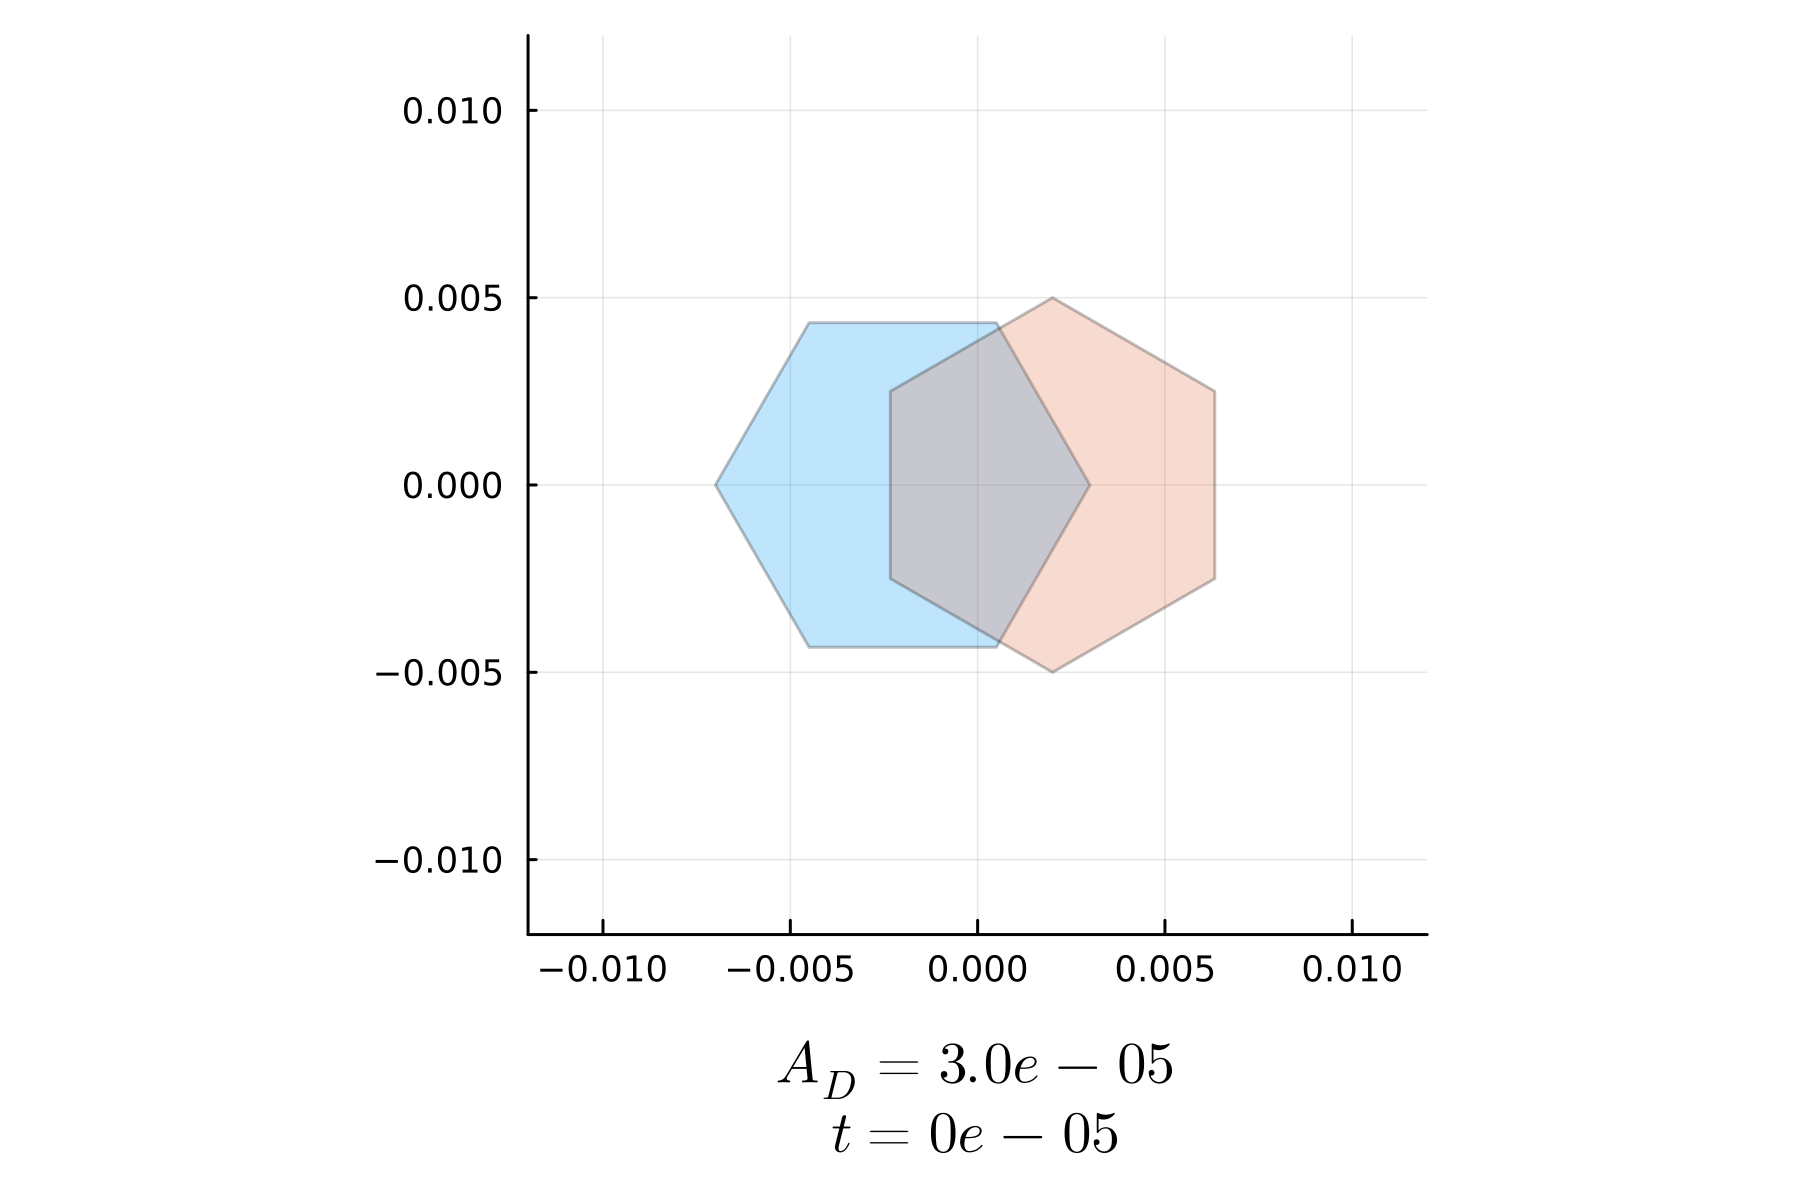
\includegraphics[width=0.5\textwidth]{forces/defOverlap1/t0.png} &
        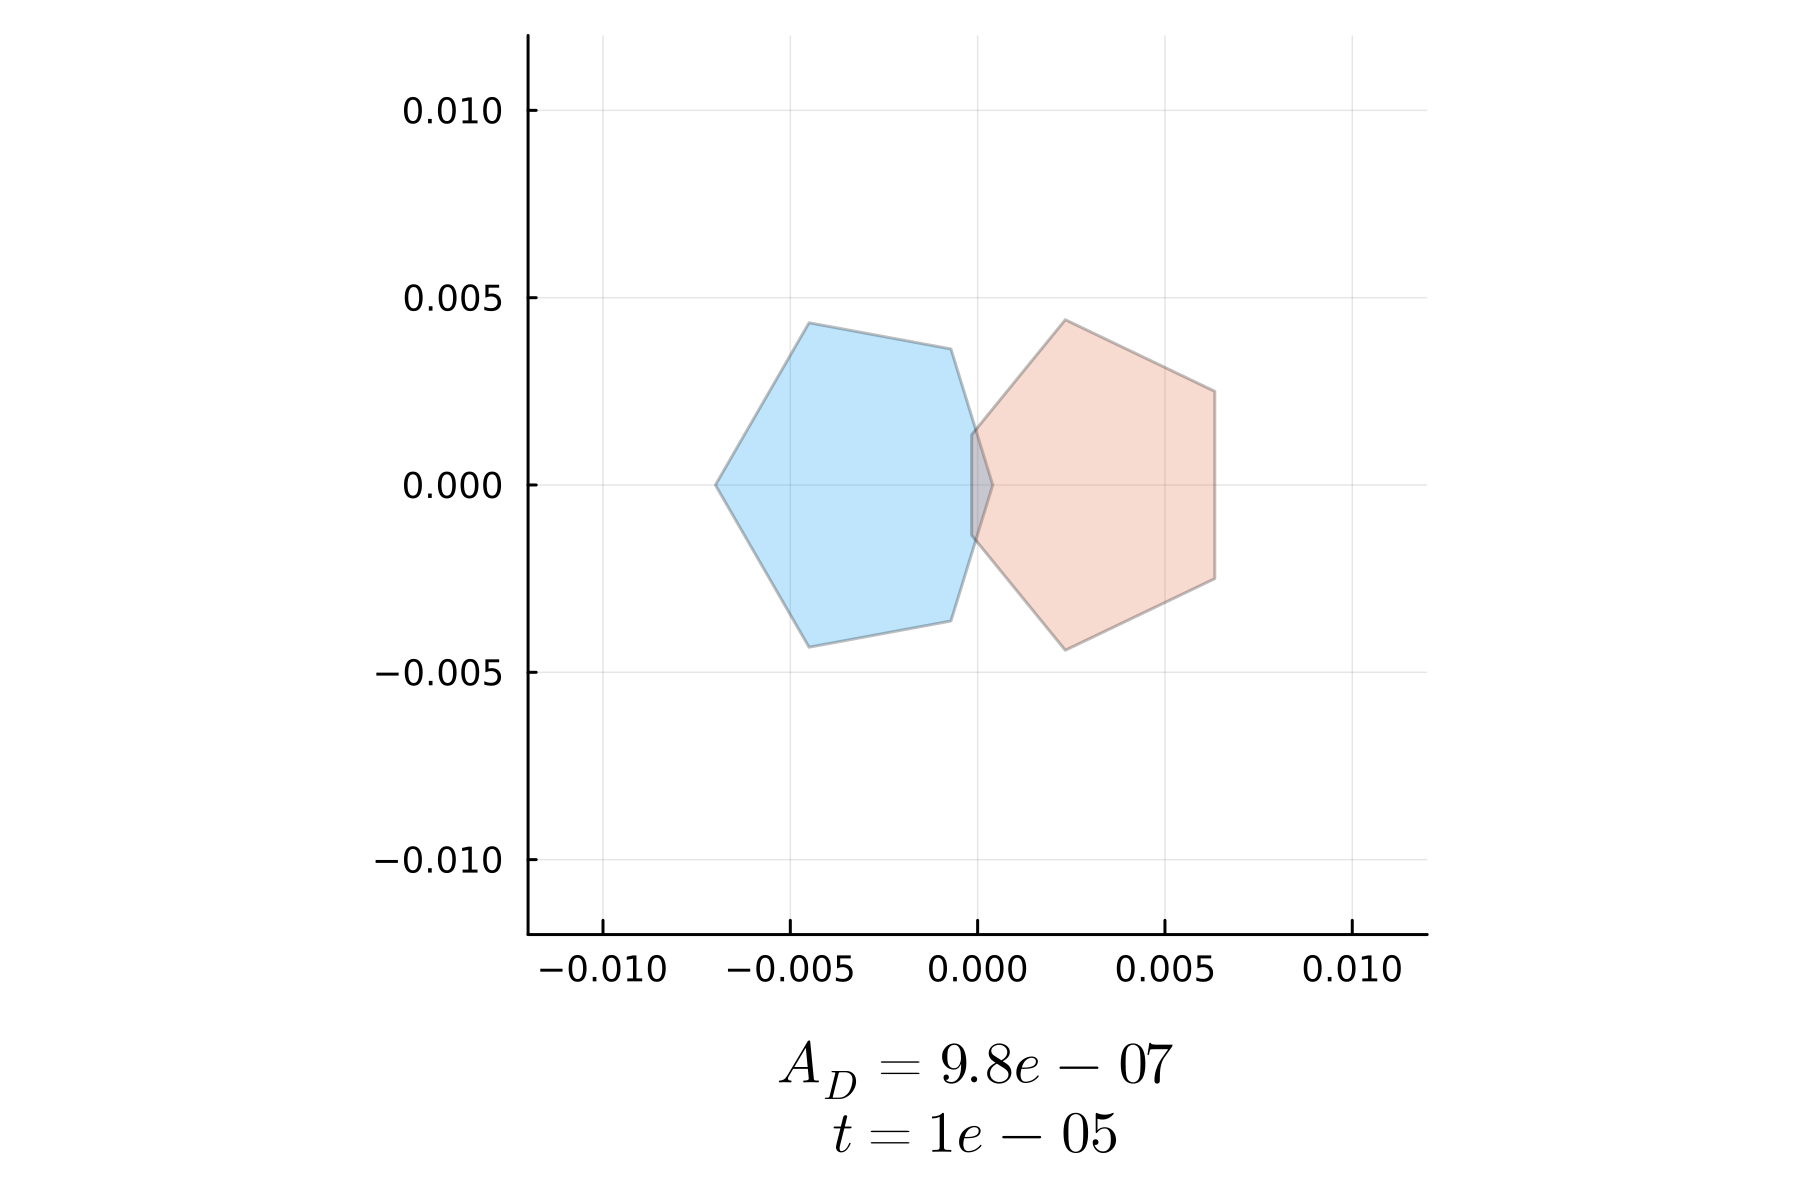
\includegraphics[width=0.5\textwidth]{forces/defOverlap1/t1.png} \\
        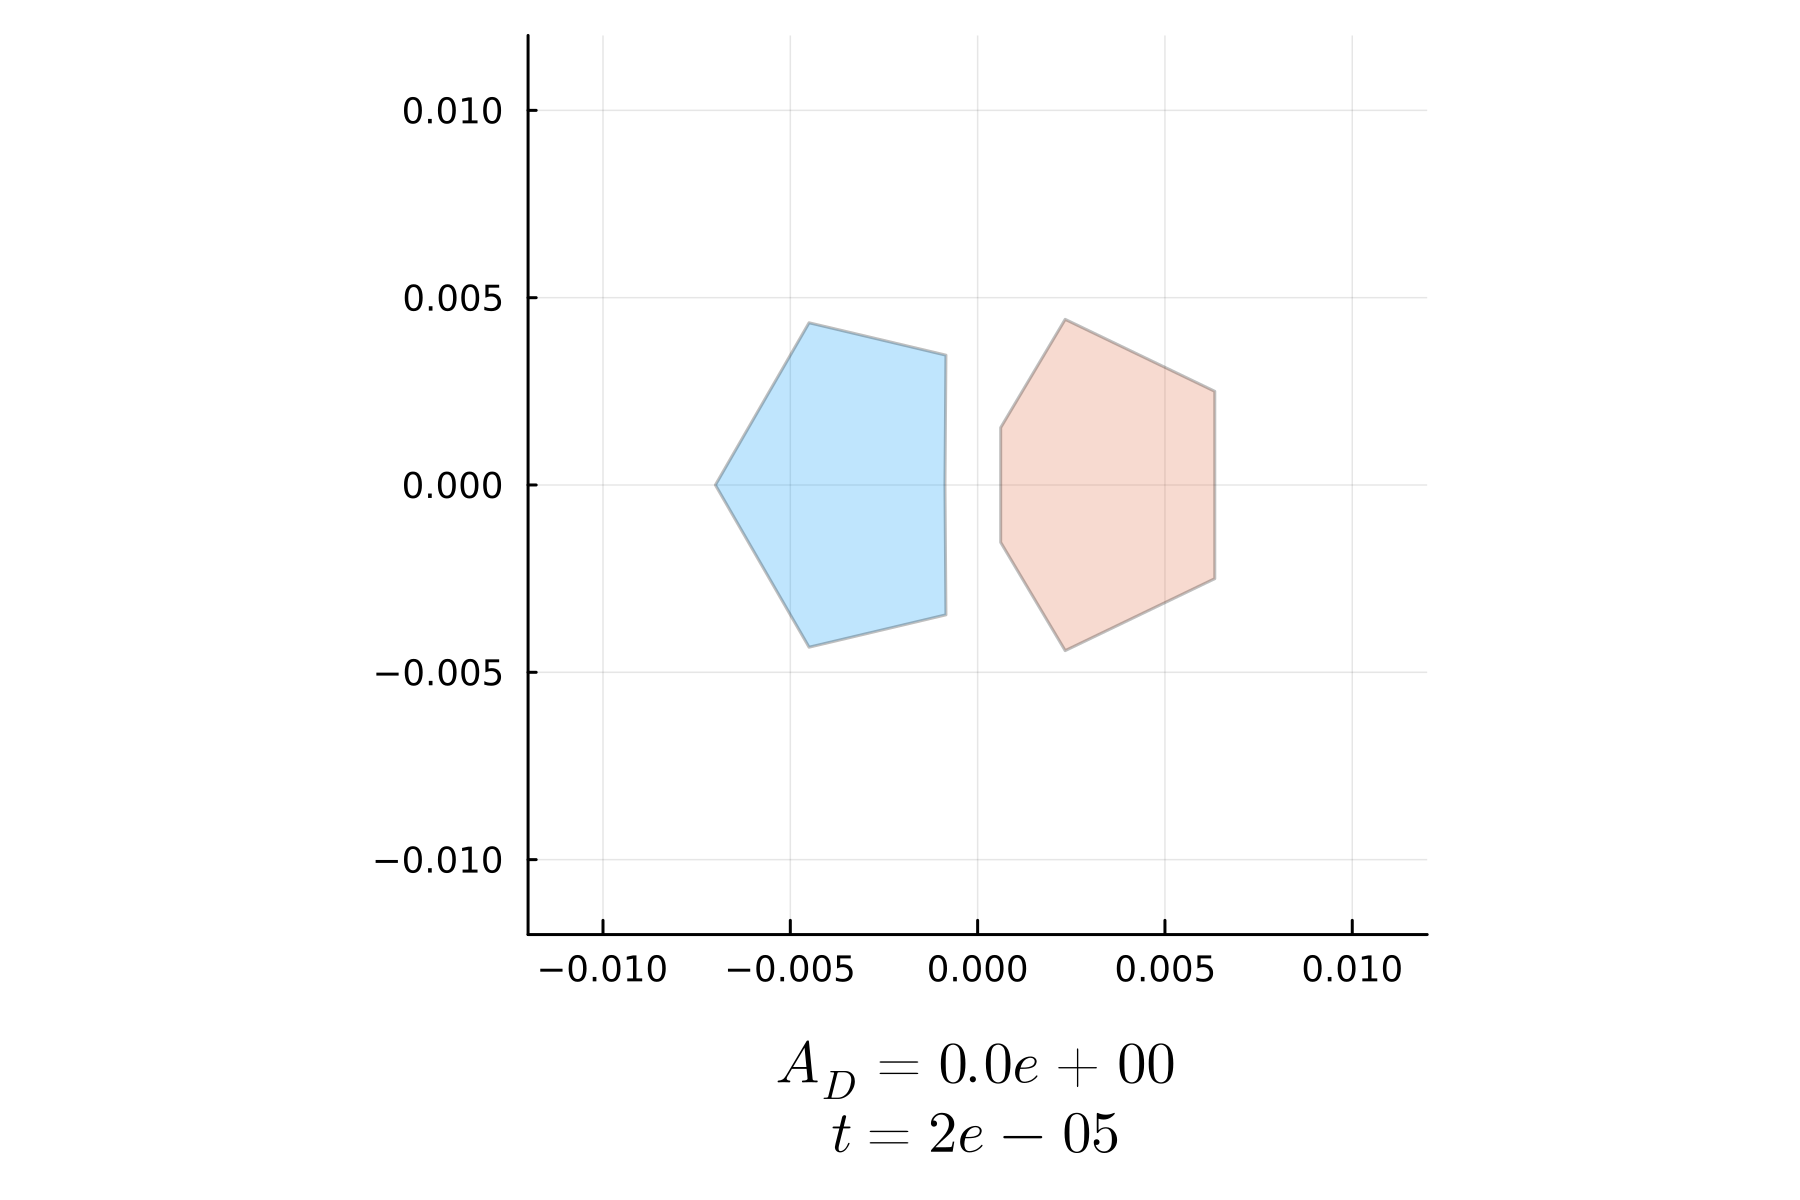
\includegraphics[width=0.5\textwidth]{forces/defOverlap1/t2.png} &
        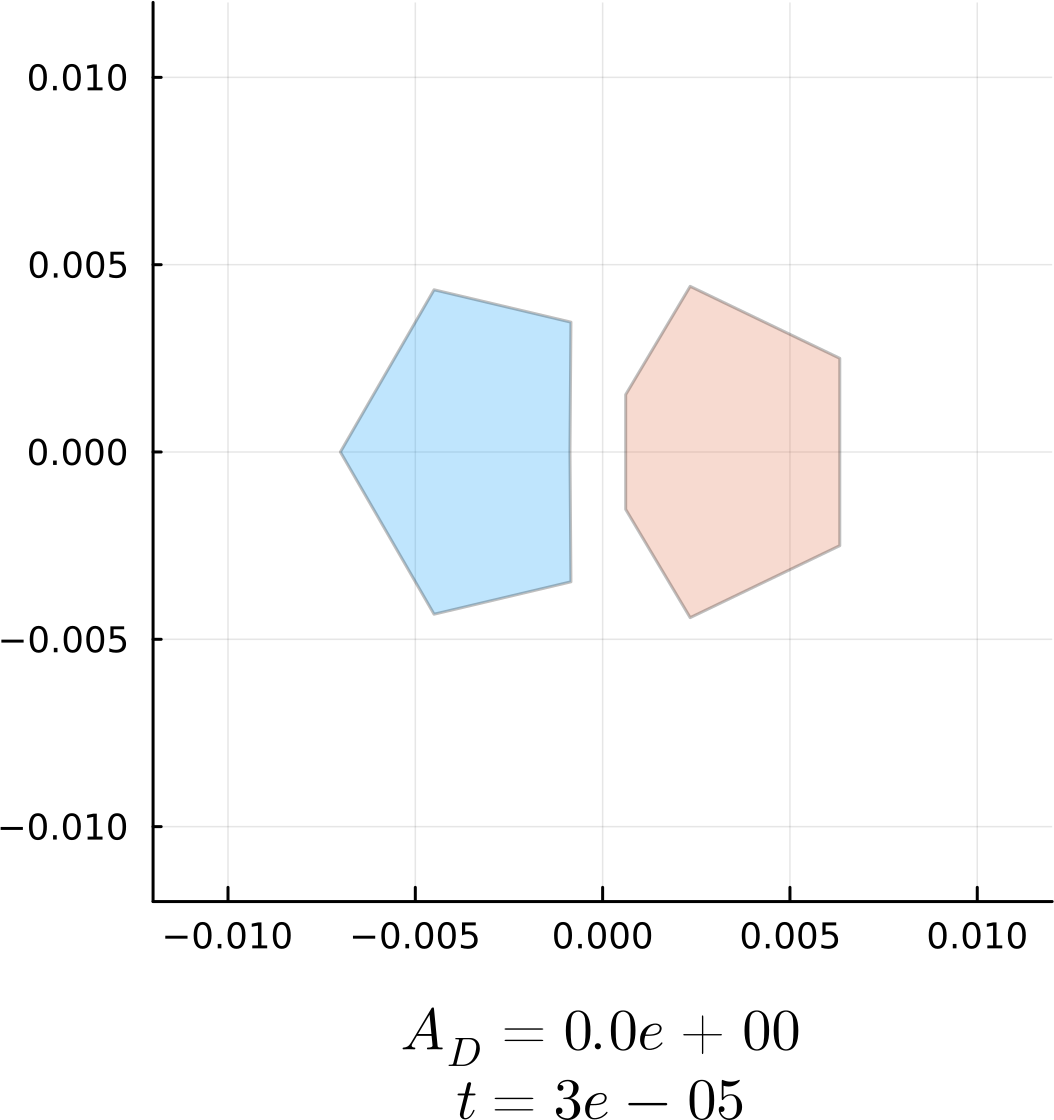
\includegraphics[width=0.5\textwidth]{forces/defOverlap1/t3.png} \\
    \end{tabular}
    \caption{
			The top four plots show the evolution of a DF cell influenced solely by the deforming overlap force, with $k=1$ applied to the vertices and a force scaling of $6\times 10^{4}$, at times $t \in \{0, 1\times 10^{-5}, 2\times 10^{-5}, 3\times 10^{-5}\}$.\\
			In this case, we have $\frac{\dequ \vec{v}}{\dequ t} = - 6\times 10^{4} \nabla_{\vec{v}} \hat{O}_1(C_1, C_2)$ for all vertices.
			The overlap area $D$ is indicated below each plot.
			Click \href{https://github.com/tivo476c/FlexibleCellModel/blob/master/figures/gifs/showForces/show-DeformaingOverlapForce.gif}{\textit{here}} to view the corresponding animation (GIF).\\
			Initially, the overlap area is $3\times 10^{-5}$, which is relatively large compared to the cell area of $6.5\times 10^{-5}$. 
			However, it is completely resolved after just two time steps, as also illustrated in the energy diagram in Figure~\ref{fig:defOverlapEnergyDiagram}.
		}
	\label{fig:deformingOverlapForce}
\end{figure}
\begin{figure}[h!]
    \centering
        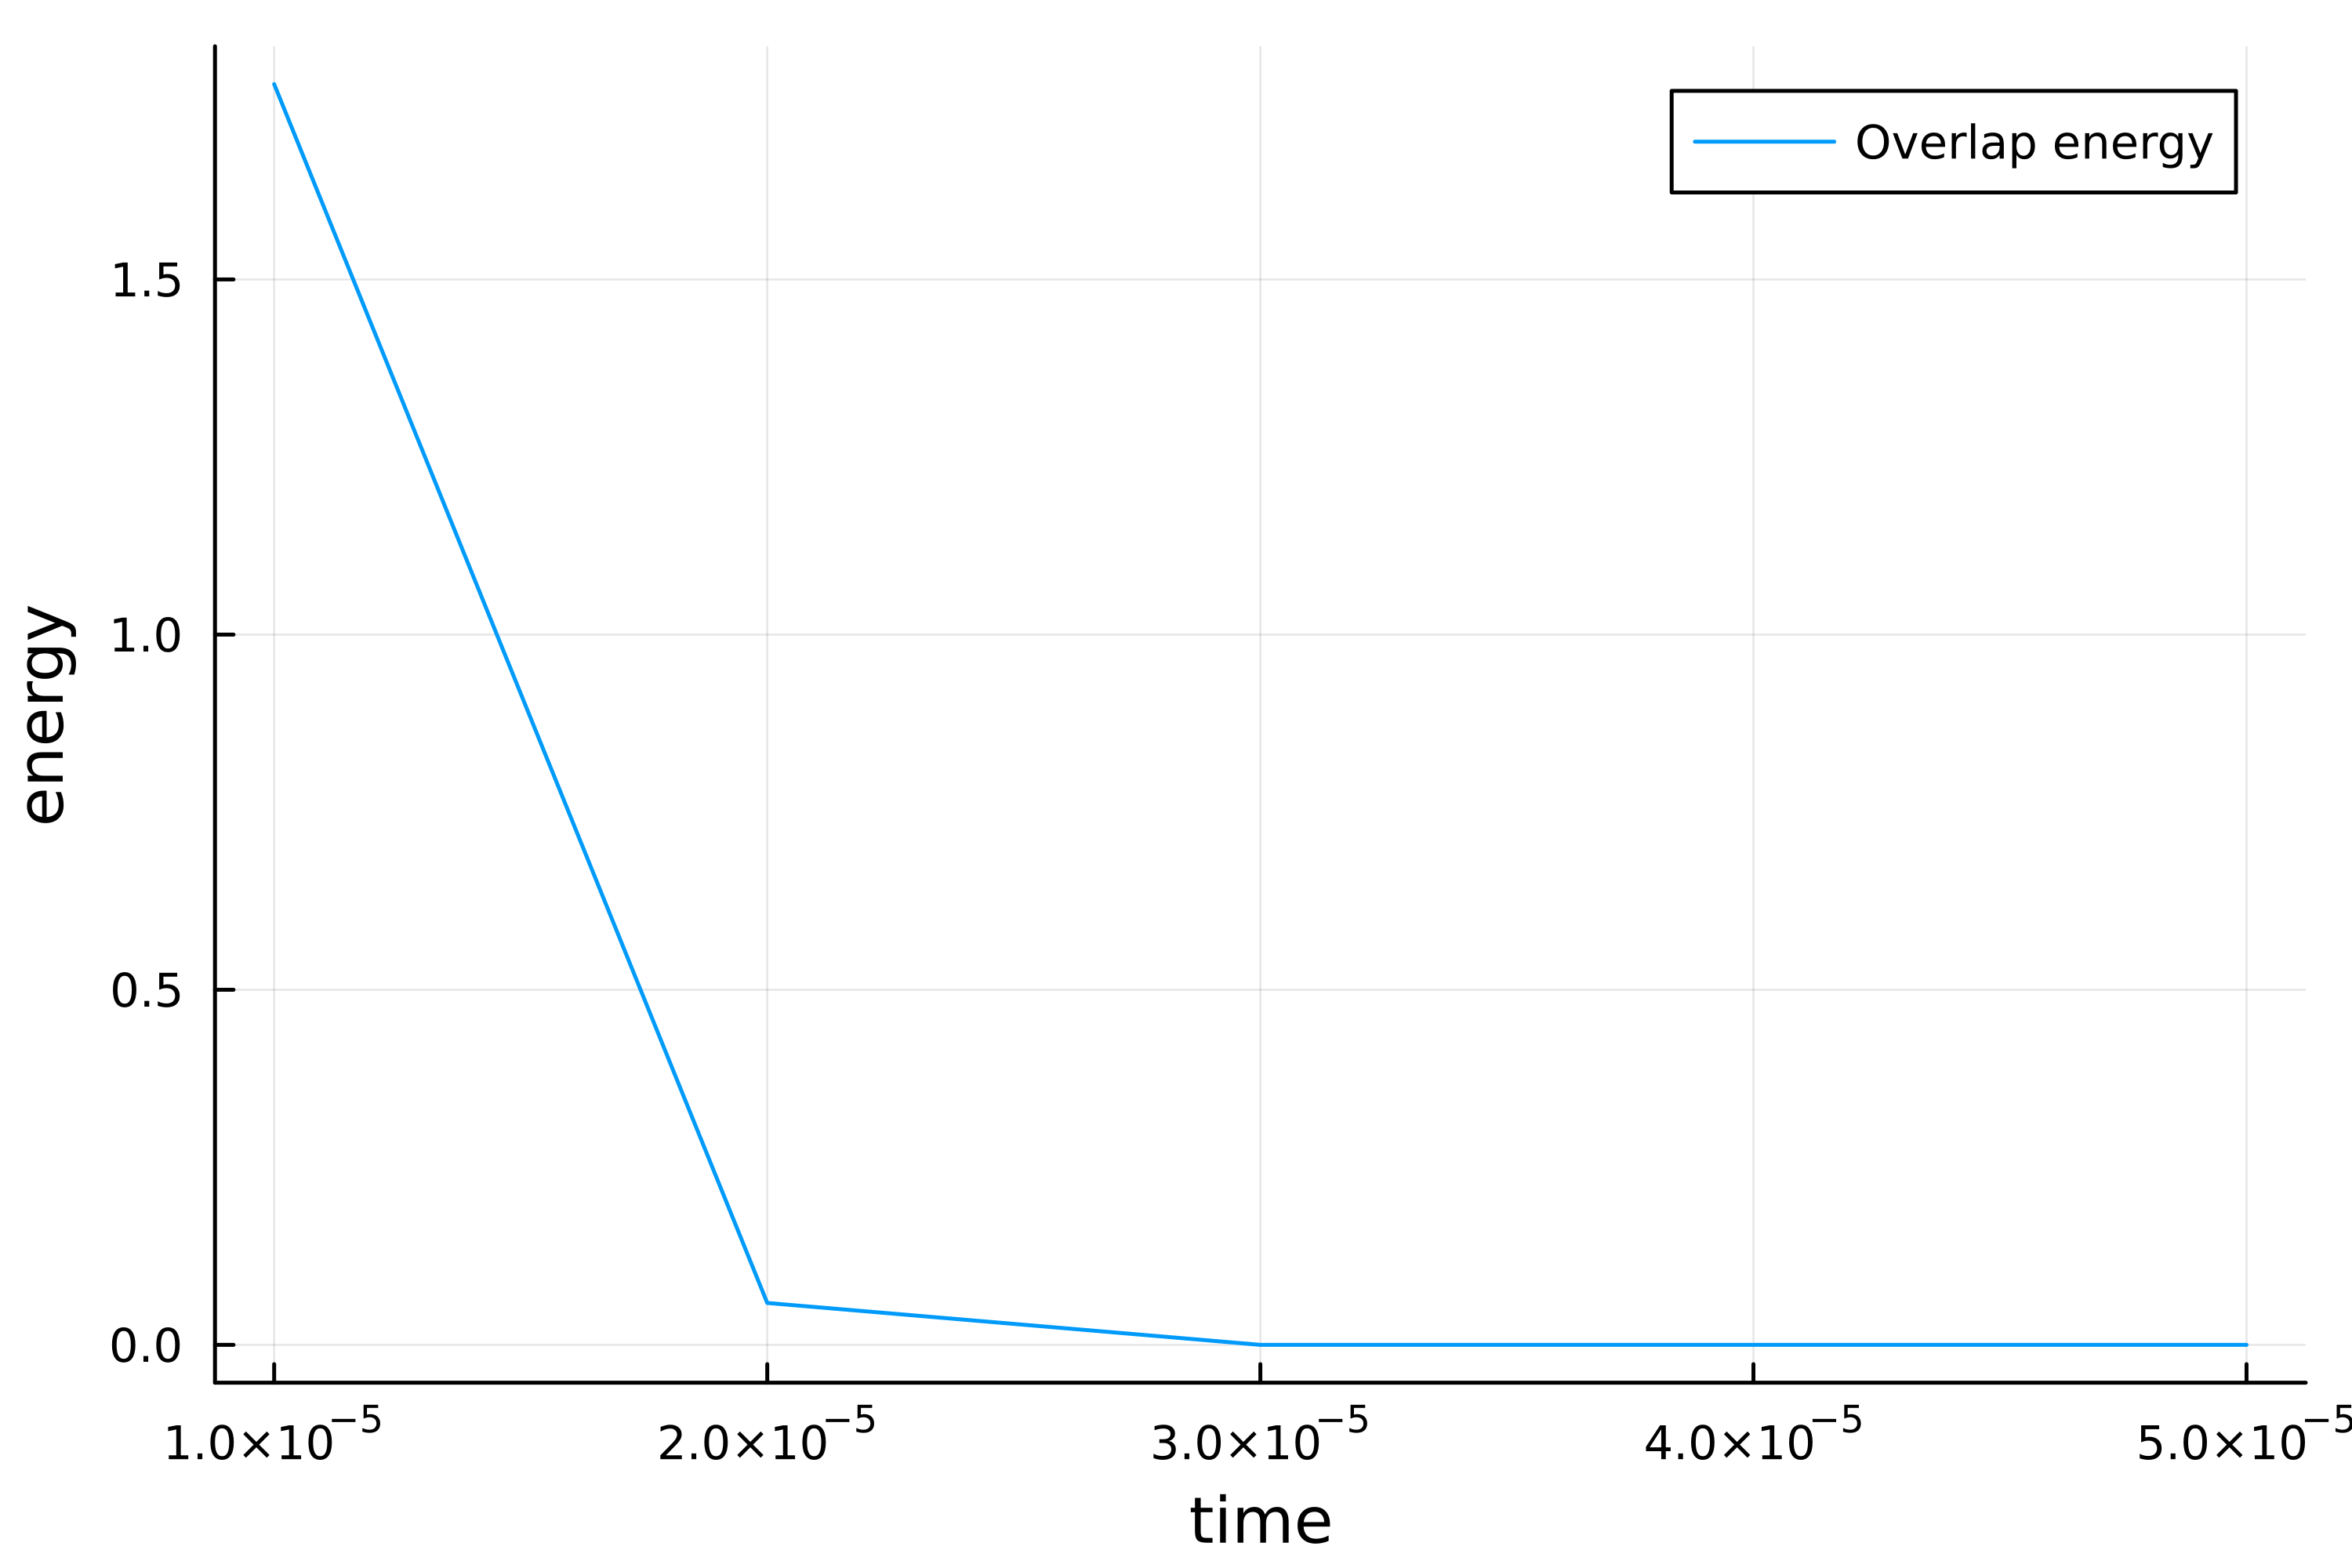
\includegraphics[width=0.7\textwidth]{forces//defOverlap1/energies-show-DeformaingOverlapForce.png} 
    \caption{The deforming overlap force resolves the overlap in two time steps.}
	\label{fig:defOverlapEnergyDiagram}    
\end{figure}


\subsubsection*{Bounce overlap force} 
While the previously introduced overlap force effectively reduces cell overlap by deforming the cells' shapes, it does not directly separate them spatially—leaving cells temporarily stuck together, relying on random Brownian motion to diffuse apart. 
With just that force, it is hard to compare the DF cell model to the hard sphere cell model, where overlaps are solved by reflecting them away from each other, resulting in a real distance that both cells have after a really small amount of time. \\  
To address this limitation and ensure a smoother conceptual and mechanical transition from the hard disc cell model, where non deformable cells simply bounce off one another, we introduce a second overlap degeneration force. 
This additional force, which we refer to as the bounce overlap force, acts not by changing cell shape but by actively transporting overlapping cells away from each other. 
This mechanism captures the spatial repulsion characteristic of rigid body interactions while complementing the shape based degeneration of overlaps in deformable cells. 
In the end, we will use a combination of both overlap forces to get a nice transition from the HCSM to the DF cell model. \\ 
In~\cite{Bruna2012} overlapping cells with a radius of $r$ that have a centre-to-centre distance of $2r - a$ will be reflective apart in one time step (that is $10^{-5}$), resulting in a distance of $2r + a$ between the two cell centres afterwards. \\
The following force does the exact same for our DF cells. 
But we need the following assumptions:
\begin{enumerate}
	\item Our DF cells model circular discs. 
	\item The cells have a radius of $r \in \R_{>0}$.
	\item We can compute the cell centre $\vec{x} = \frac{1}{N_V}\sum\limits_{j = 1}^{N_v} \vec{v}_j$ which will be used to determine the distance between two cells. 
\end{enumerate}

\begin{definition}\textbf{Bounce overlap force} \\
	Let us consider two DF cells $C_i$ and $C_l$, with centres at $\vec{x}_i$ and $\vec{x}_l$, respectively. 
	We assume that each cell has a fixed radius $r > 0$.
	We define the vector $\dequ \bar{o}_{i,l} \in \mathbb{R}^2$, which is applied equally to all vertices of cell $C_i$, representing the repulsive overlap force caused by cell $C_l$. 
	It is given by
	\[
	\dequ \bar{o}_{i,l} = \mathbf{1}_{\norm[\vec{x}_i - \vec{x}_l] < 2r} (2r - \norm[\vec{x}_i - \vec{x}_l]) \dfrac{\vec{x}_i - \vec{x}_l}{\norm[\vec{x}_i - \vec{x}_l]}.
	\]
	This force is zero if the distance between the cell centres satisfies $\norm[\vec{x}_i - \vec{x}_l] \geq 2r$.

	Otherwise, if the cells overlap (i.e., $\norm[\vec{x}_i - \vec{x}_l] < 2r$), the vector $\dequ \bar{o}_{i,l}$ points from $\vec{x}_l$ to $\vec{x}_i$ and has magnitude equal to the overlap depth $a = 2r - \norm[\vec{x}_i - \vec{x}_l]$. 
	At the same time in the simulation, the same magnitude of displacement is applied to all vertices of $C_l$ in the opposite direction, i.e., along $\vec{x}_l - \vec{x}_i$.
	This means that all vertices of cell $C_i$ are displaced away from $C_l$ in the direction $\vec{x}_i - \vec{x}_l$ such that the resulting displacement is sufficient to separate the two cells' centres by exactly $2r + a$. 

	The force $F^{(\bar{O})}_{i,l}$ that acts on cell $C_i$ due to its interaction with cell $C_l$ is given by
	\[
	F^{(\bar{O})}_{i,l}(C_i, C_l) =  (\dequ \bar{o}_{i,l}, \ldots, \dequ \bar{o}_{i,l})^T \in \mathbb{R}^{2N_V},
	\]
	where the vector $\dequ \bar{o}_{i,l}$ is repeated $N_V$ times, once for each vertex of cell $C_i$.

	The total bounce overlap force $F^{(\bar{O})}_i: (\mathbb{R}^{2N_V})^{N_C} \rightarrow \mathbb{R}^{2N_V}$ acting on cell $C_i$ due to all other cells in the system is then defined as
	\[
	F^{(\bar{O})}_i(\vec{C}) = \sum\limits_{l \neq i} F^{(\bar{O})}_{i,l}(C_i, C_l).
	\]

\end{definition}
In order to achieve a similarly fast degeneration of the overlap as in~\cite{Bruna2012}, we need to scale the force with the scaling factor 
\(
\alpha^{(\bar{O})} = 10^5
\)
as the time needed to resolve such an overlap in~\cite{Bruna2012} was always one time step which is $10^{-5}$. 

%TODO: insert figure of Bounce overlap force 
To account for varying cell stiffness, we introduce a new parameter $h \in [0, 1]$ that controls how `hard' the cells are. 
The total overlap force is then defined as a weighted combination of two overlap force types:
\[
F^{(\mathbf{O})} = h \cdot F^{(\bar{O})} + (1 - h) \cdot F^{\hat{(O)}},
\]
where $F^{(\bar{O})}$ denotes the bounce-off overlap force and $F^{\hat{(O)}}$ the shape-deforming overlap force.\\
When $h = 1$, the cells are maximally stiff. 
In this case, shape deformation is entirely suppressed: all overlaps are resolved solely through the bounce off mechanism, and the shape preserving forces become redundant since the cells always retain their desired configurations. \\
As $h$ decreases, the cells become progressively softer. 
The influence of the bounce-off force diminishes, while the shape-deforming overlap force gains dominance, allowing cells to deform more in response to contact with neighbors. \\
With the introduction of the hardness parameter $h$, we have established a mechanism that enables a smooth transition from the HSCM dynamics introduced in~\cite{Bruna2012} to our new DF cell model. \\
For $h = 1$, the dynamics are identical to the original HSCM model, as we will show in the following chapter. 
By gradually decreasing $h$, we can continuously adapt the system behavior toward the pure deformable (DF) cell model. 
In this way, we can systematically investigate how the dynamics evolve between the two regimes. 
In the limiting case $h = 0$, we recover the DF dynamics without the bounce overlap force term.

\begin{figure}[h!]
    \centering
    \begin{tabular}{cc}
        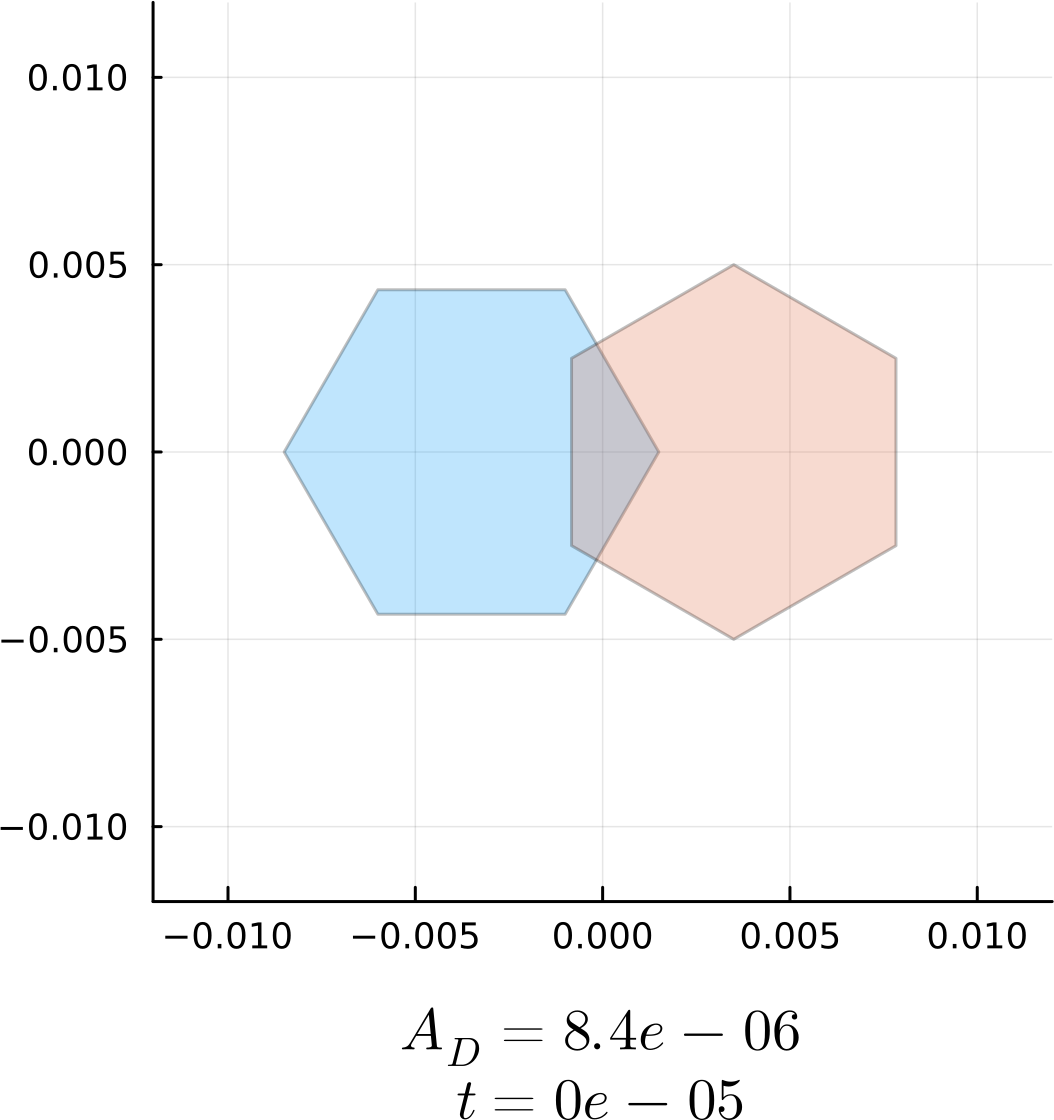
\includegraphics[width=0.5\textwidth]{forces/bounceOverlap1/t0.png} &
        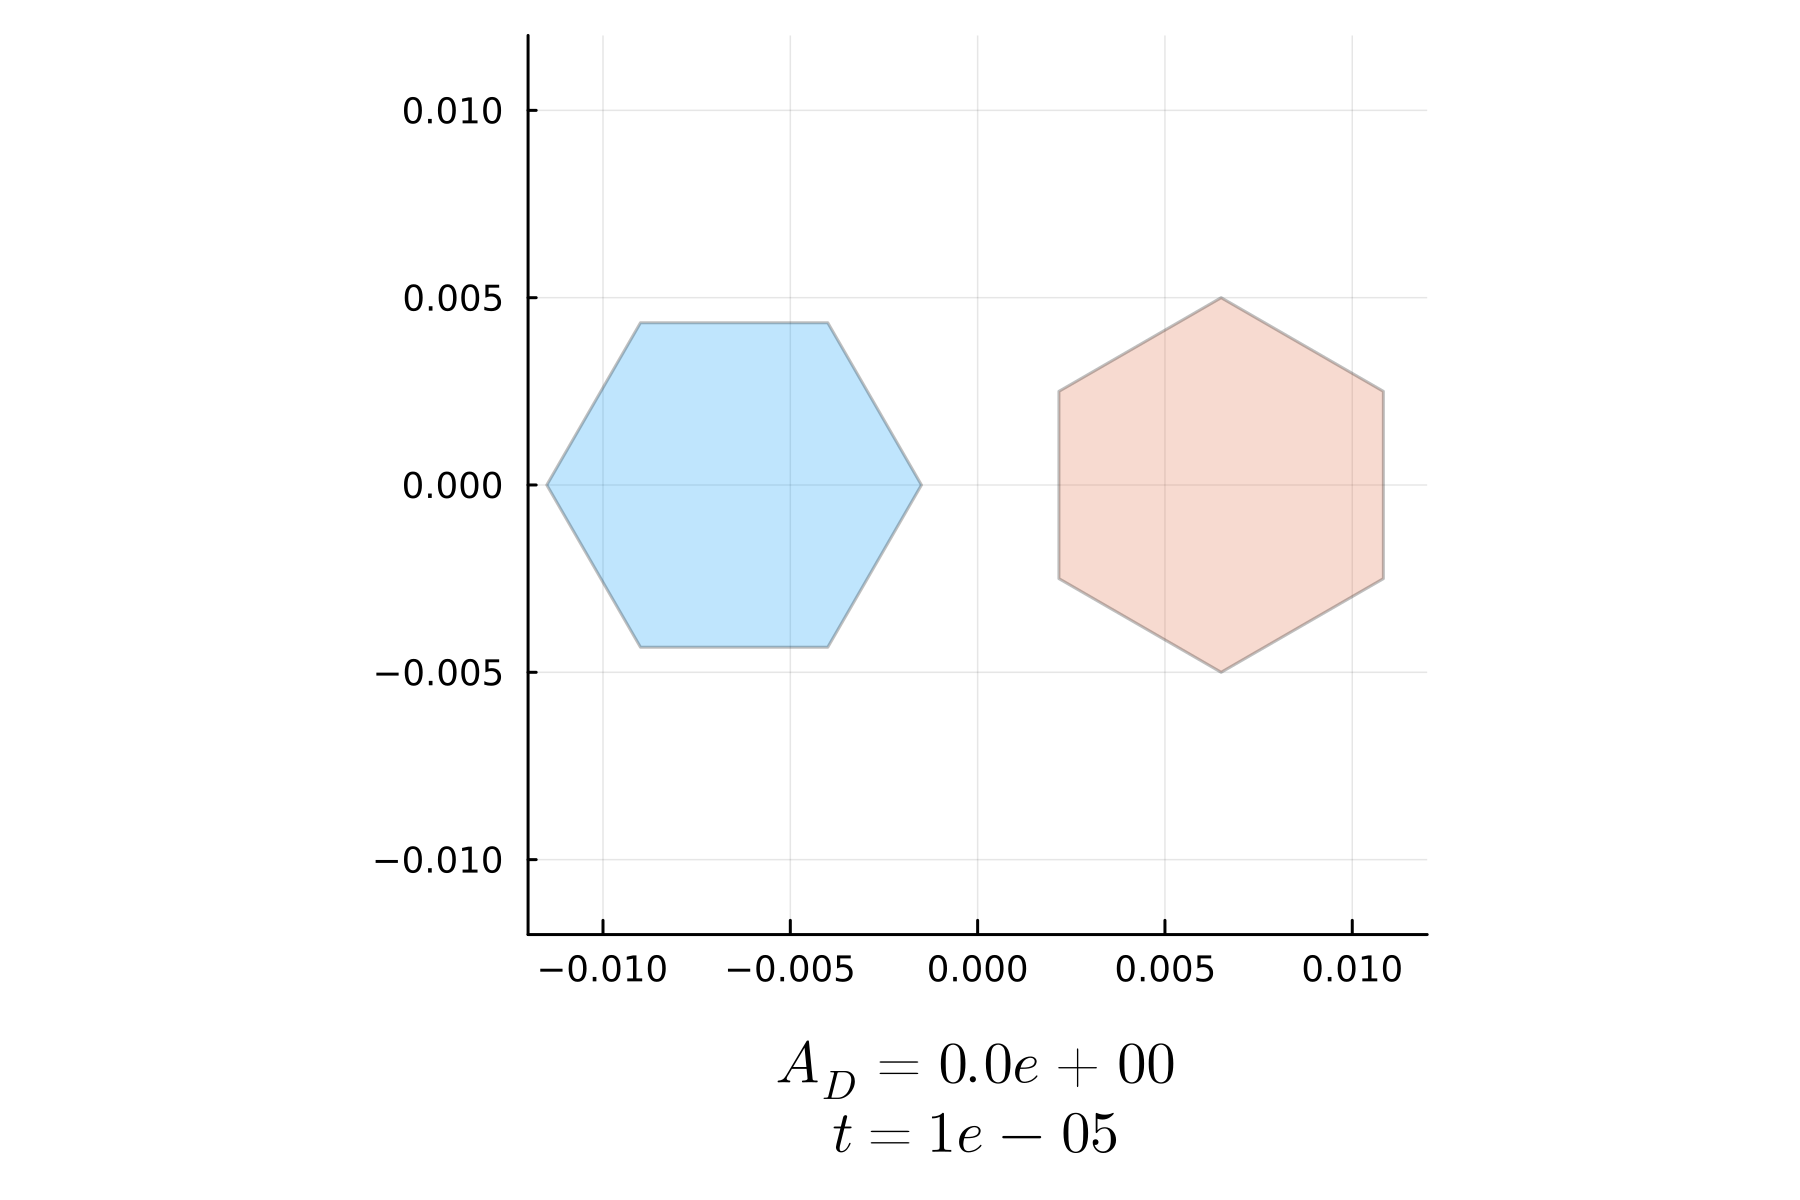
\includegraphics[width=0.5\textwidth]{forces/bounceOverlap1/t1.png} \\
        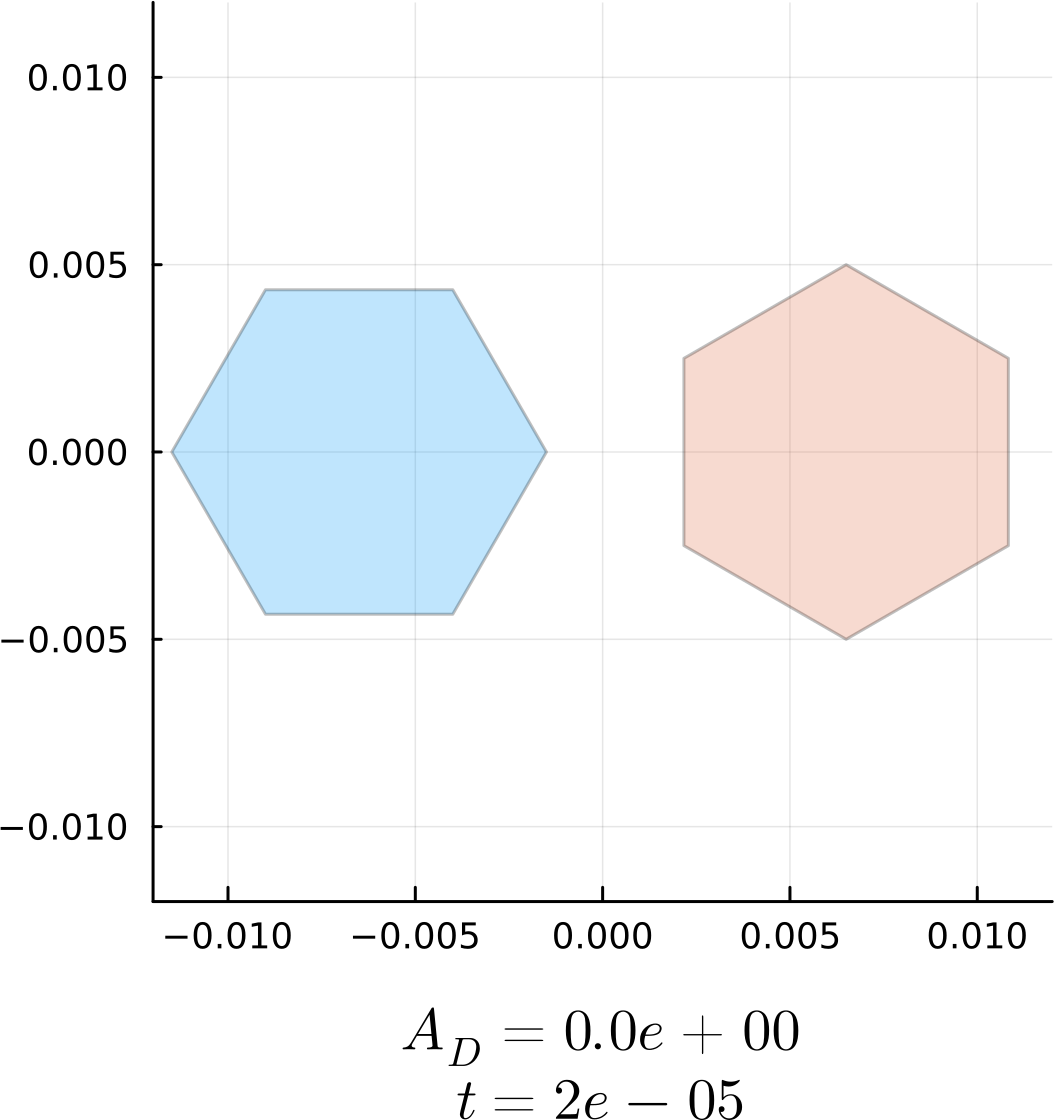
\includegraphics[width=0.5\textwidth]{forces/bounceOverlap1/t2.png} &
        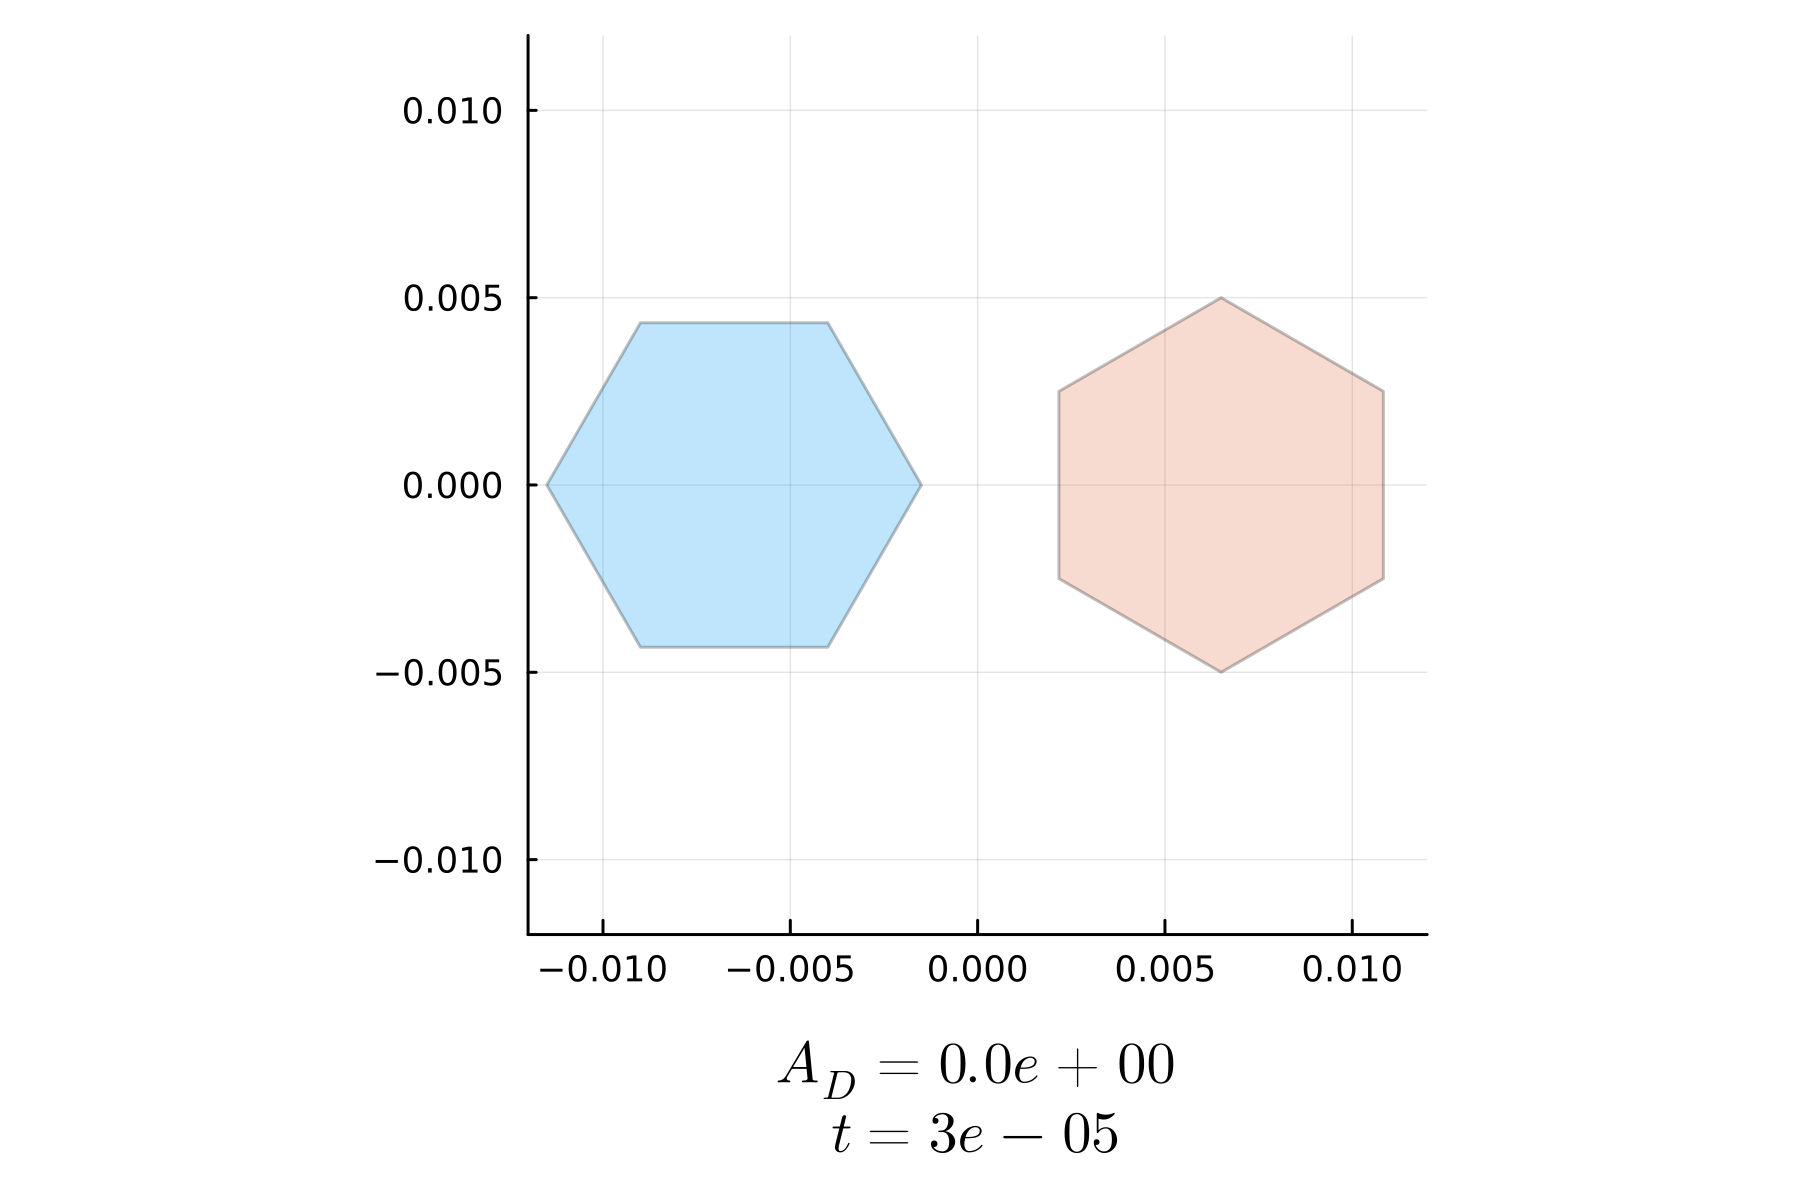
\includegraphics[width=0.5\textwidth]{forces/bounceOverlap1/t3.png} \\
    \end{tabular}
    \caption{The top four plots present the evolution of a DF cell governed solely by the bounce overlap force, applied to the vertices with a force scaling of $1\times 10^{5}$, at times $t \in \{0, 1\times 10^{-5}, 2\times 10^{-5}, 3\times 10^{-5}\}$.\\
			In this case, we have $\frac{\dequ C_i}{\dequ t} = 1\times 10^{5} \: F_i^{\bar{O}}(C_1, C_2)$ for both cells.
			Click \href{https://github.com/tivo476c/FlexibleCellModel/blob/master/figures/gifs/showForces/show-bounceOverlapForce.gif}{\textit{here}} to view the corresponding animation (GIF).\\
			The overlap vanishes within the very first time step, leaving a visible gap between the two cells. 
			The corresponding energy development is illustrated in Figure~\ref{fig:bounceOverlapEnergyDiagram}.
		}
	\label{fig:bounceOverlapForce}   
\end{figure}
\begin{figure}[h!]
    \centering
        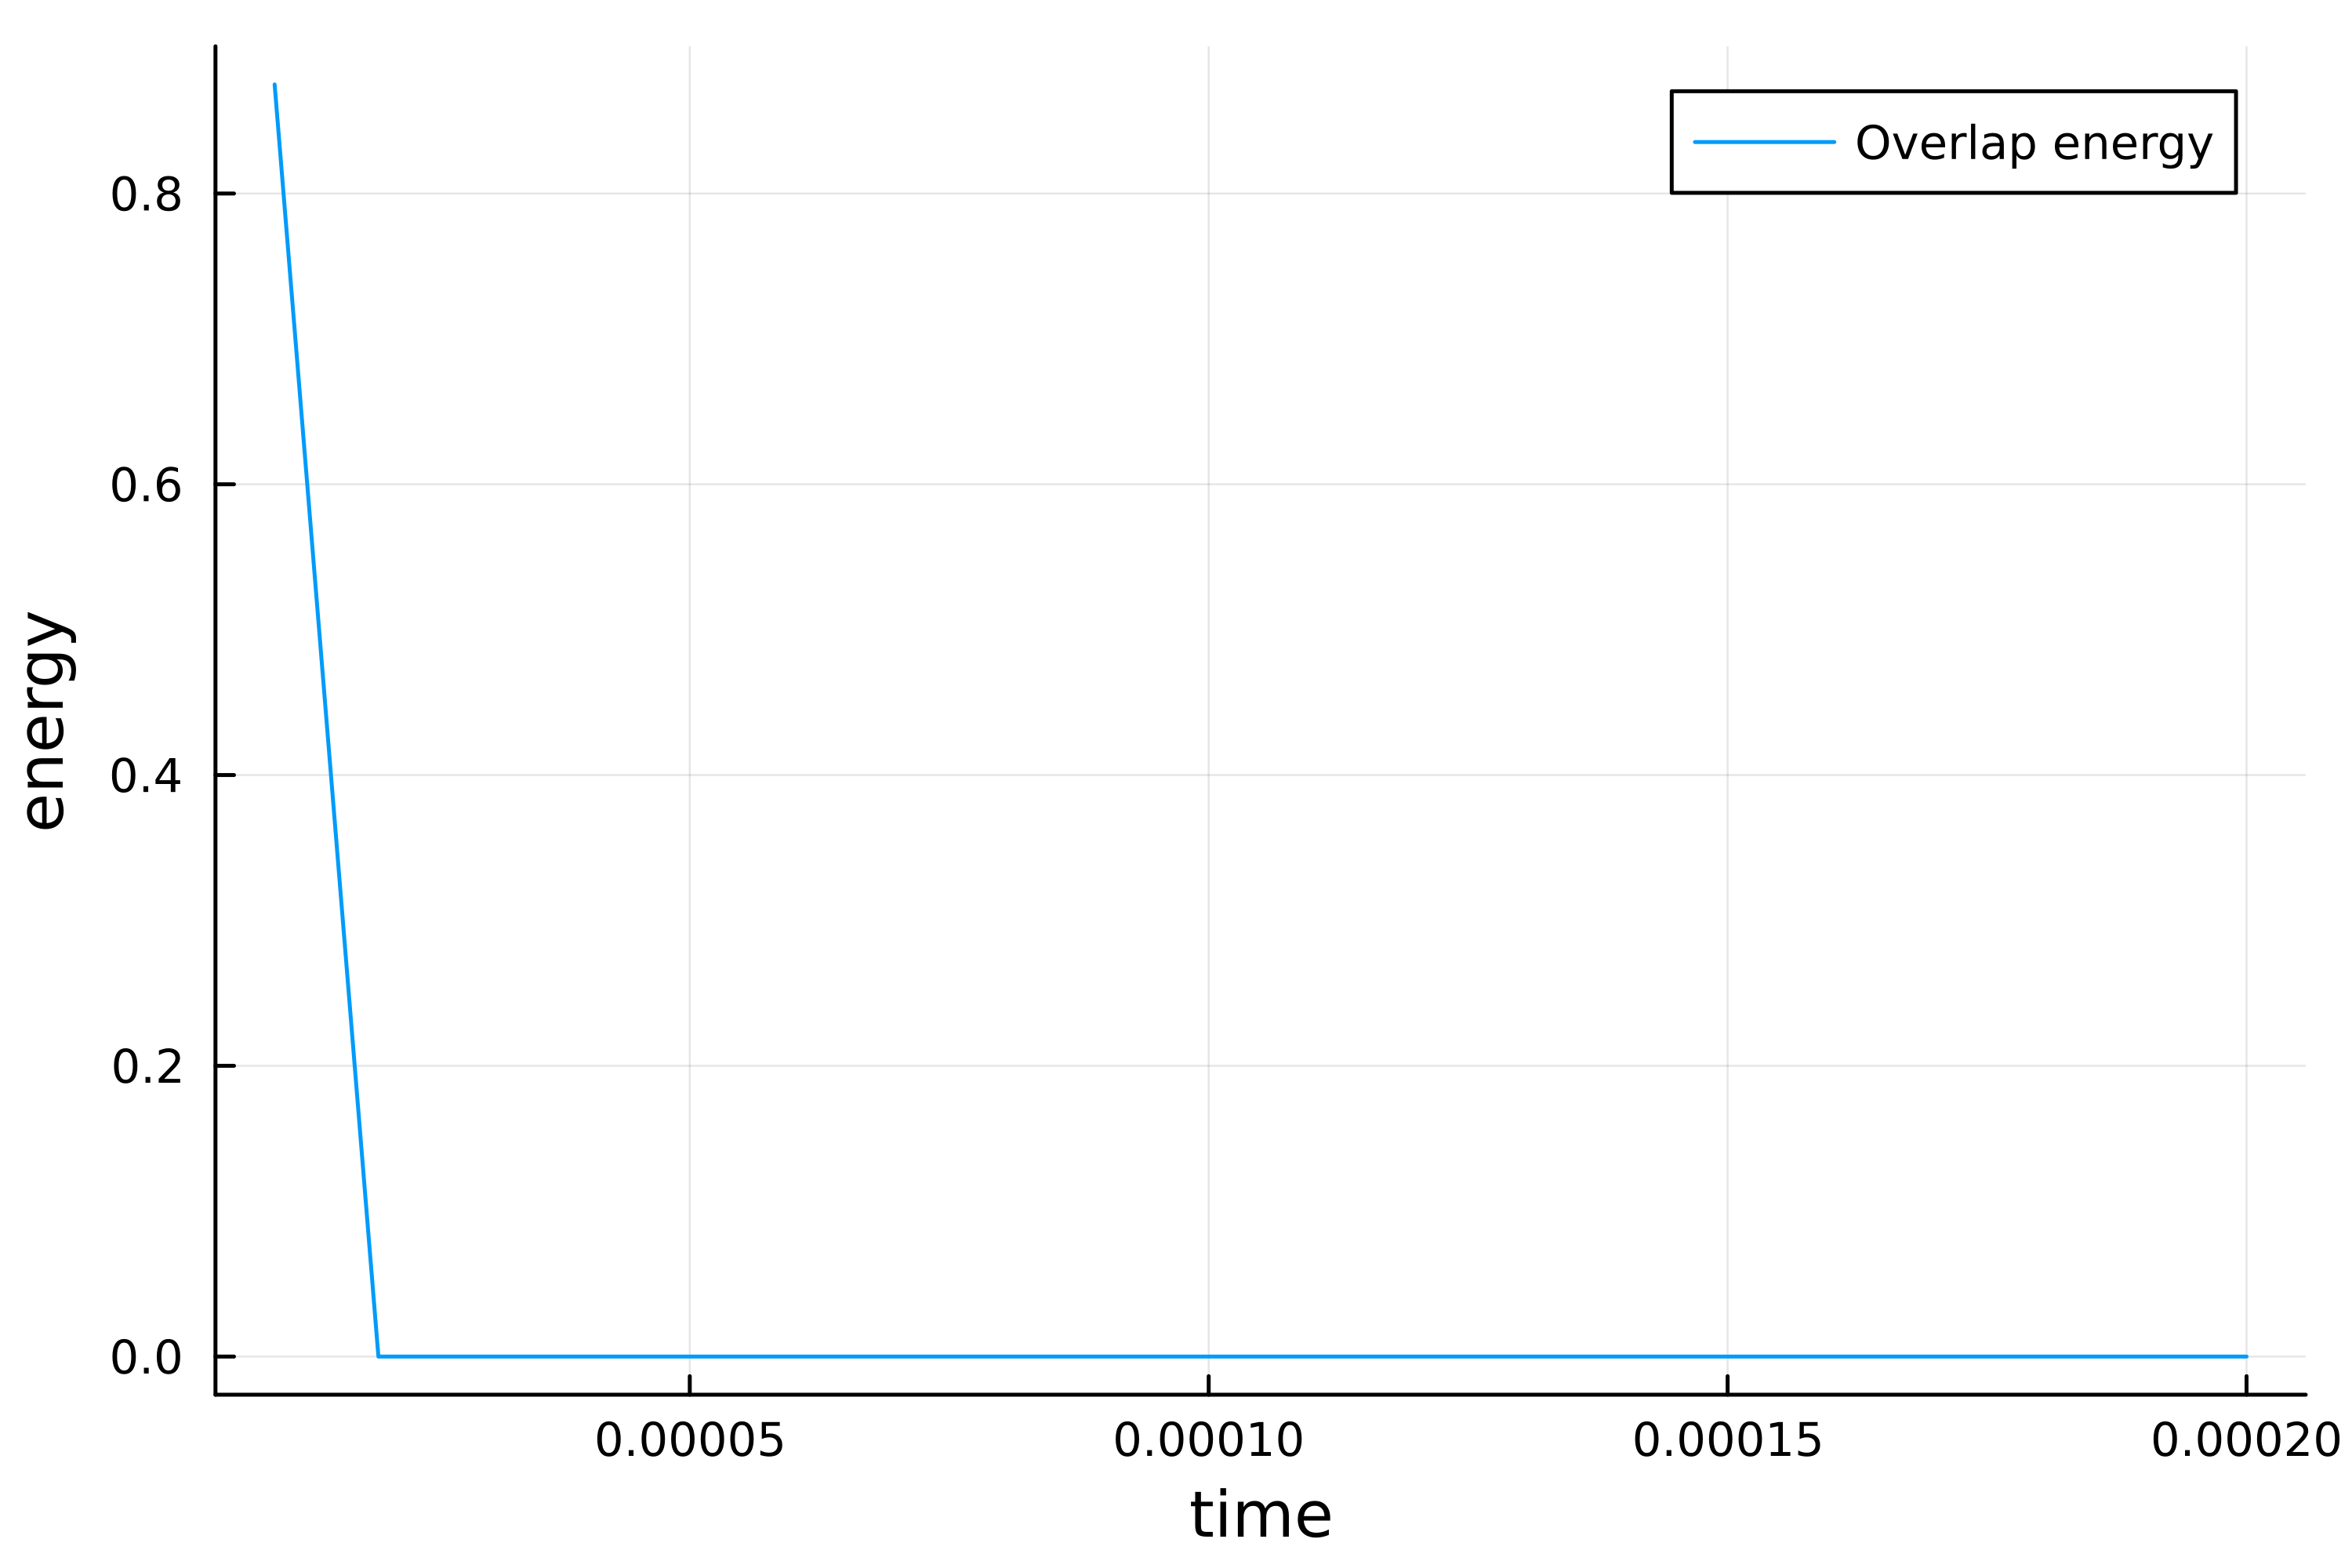
\includegraphics[width=0.7\textwidth]{forces/bounceOverlap1/energies-show-bounceOverlapForce.png} 
    \caption{The overlap energy reaches zero after one iteration.}
	\label{fig:bounceOverlapEnergyDiagram}    
\end{figure}




\subsection{The DF SDE}
Having defined all individual force contributions acting on the cell vertices, we now combine them to formulate the full dynamics of the system in terms of a stochastic differential equation. \\
One challenging aspect that remains is the appropriate scaling of all forces.
It has become evident that the system is highly sensitive to these scaling parameters. 
If the shape-recovering forces are too small, the recovery process is excessively slow. 
Conversely, if they are too large, the numerical integration scheme tends to become unstable. \\ 
To ensure numerical stability while preserving the intended dynamics, we systematically tested the appropriate scaling for each force type, focusing in particular on the shape-preserving forces and the deforming overlap force.

Our method was to isolate each of these forces in simulation and determine the threshold at which the system becomes unstable. 
Specifically, we ran simulations with only one force active at a time and gradually increased its scaling factor until numerical instabilities emerged. 
We then selected the **maximum stable scaling** as the operative value for that force. \\
These tests were conducted using a fixed time step of $10^{-5}$, with cell configurations composed of six vertices. 
To rigorously challenge the model, we initialized the cells in deliberately distorted and uncomfortable shapes, which are most prone to triggering instabilities. 
The configurations used in these tests are the same as those shown in the figures throughout this chapter, where the isolated effects of each force were illustrated following their respective introductions. 
This allowed us to verify that the chosen scalings are robust even under unfavorable conditions. \\
For the bounce overlap force, a scaling factor of $10^5$ is necessary to reproduce the original bounce off dynamics used in~\cite{Bruna2012}. \\
Summarizing all these efforts, we arrived at the following force scalings used in the simulations:

\begin{table}[h]
	\centering
	\begin{tabular}{|c|c|}
		\hline
		\textbf{Force type} & \textbf{Scaling parameter} \\
		\hline
		\text{Area force} & $\alpha_A = 4.0 \times 10^8$ \\
		\text{Edge force} & $\alpha_E = 3.0 \times 10^4$ \\
		\text{Interior angle force} & $\alpha_I = 1.0 \times 10^{-1}$ \\
		\text{Deforming overlap force} & $\alpha_{\hat{O}} = 6.0 \times 10^4$ \\
		\text{Bounce overlap force} & $\alpha_{\bar{O}} = 1.0 \times 10^5$ \\
		\hline
	\end{tabular}
	\caption{Scaling parameters for different force types}
	\label{table:forcescalings}
\end{table}

These scaling par
ameters serve as the foundation for the complete DF SDE model, which we now introduce.
\begin{definition} \textbf{The DF SDE} \\
	We define the vectors
	\[
	e_{N_V}^{x} = (1,0,1,0,\ldots,1,0)^T, \quad e_{N_V}^{y} = (0,1,0,1,\ldots,0,1)^T \in \R^{2N_V},
	\]
	which allow us to distribute a two dimensional Brownian motion \[\dequ \vec{B}^{\:i}_t = (\dequ B^{i,x}_t, \dequ B^{i,y}_t)^T\] to the $x$ and $y$ coordinates of a cell's vertices, respectively.
	The cell hardness parameter $h \in [0,1]$ is assumed to be given.
	The deterministic part $F^{i}(\vec{C})$ of the \textbf{DF SDE} is given by 
	\begin{center}
		$ \F^i: (\R^{2N_V})^{N_C} \rightarrow \R^{2N_V} $
	\end{center}
	\begin{align}
		\begin{split}
			\F^{i}(\vec{C}) = \; & \alpha_{A} F_2^{(A)}(C_i) + \alpha_{E} F_2^{(E)}(C_i) + \alpha_{I} F_2^{(I)}(C_i) + \\
			& (1-h)\alpha_{\hat{O}} F_{1,i}^{(\hat{O})}(\vec{C}) + h \alpha_{\bar{O}} F_i^{(\bar{O})}(\vec{C})
		\end{split}
	\end{align}
	for each cell $1 \leq i \leq N_C$. \\ 
	Each scaling parameter $\alpha \geq 0$. 
	Each $F$ represents one of our forces that got defined in this chapter. 
	For the shape preserving forces, we choose $k=2$ as then the difference between current state and desired state influences the intensity of the force which is nice.
	But for the deforming overlap force, we choose $k=1$ we want it to have a strong impact whenever a small overlap arises. 
	This configuration seems to be the best to model the physics we would like to achieve. 
	With that we can write down the cell wise formulated DF SDE:
	\begin{center}
		$\dequ C_i = \F^{i}(\vec{C}) \dequ t + \dequ B^{i,x}_t \: e_{N_V}^{x} + \dequ B^{i,y}_t \: e_{N_V}^{y}.$
	\end{center} 


\end{definition}

\begin{figure}[h!]
    \centering
    \begin{tabular}{cc}
        \includegraphics[width=0.5\textwidth]{forces/allforces_hard/t0.png} &
        \includegraphics[width=0.5\textwidth]{forces/allforces_hard/t1.png} \\
        \includegraphics[width=0.5\textwidth]{forces/allforces_hard/t2.png} &
        \includegraphics[width=0.5\textwidth]{forces/allforces_hard/t3.png} \\
    \end{tabular}
    \caption{
		This simulation shows two DF cells evolving according to the dynamics for $i = 1, 2$
		$\frac{\dequ C_i}{\dequ t} = \F^i(C_1, C_2)$ with hardness $h=1$, force scalings as listed in Table~\ref{table:forcescalings} and without Brownian motion.
		Click \href{https://github.com/tivo476c/FlexibleCellModel/blob/master/figures/gifs/showForces/show-allForces-hard.gif}{\textit{here}} to view the corresponding animation (GIF).
		The cells are initially generated with overlap. 
		Then, the dynamics from $\F^i$ alone resolve the overlap.
		Since hardness $h=1$ was chosen, no deforming overlap force is active and the cell shape remains unchanged. 
		Consequently, the shape-preserving forces are inactive, as the cells stay in their desired states.\\
		This is also reflected in the energy diagram in Figure~\ref{fig:allForces-hardEnergyDiagram}. 
	}
	\label{fig:allForces-hard}
\end{figure}

\begin{figure}[h!]
    \centering
        \includegraphics[width=0.7\textwidth]{forces/allforces_hard/energies-show-allForces-hard1.png} 
    \caption{The bounce overlap force eliminates the overlap within a single time step.
			 The energy diagram shows that the overlap energy drops to zero immediately, while the other energies remain constant at zero as the cell shapes do not change.}
	\label{fig:allForces-hardEnergyDiagram}    
\end{figure}


\begin{figure}[h!]
    \centering
    \begin{tabular}{cc}
        \includegraphics[width=0.5\textwidth]{forces/allforces_0-5/t0.png} &
        \includegraphics[width=0.5\textwidth]{forces/allforces_0-5/t1.png} \\
        \includegraphics[width=0.5\textwidth]{forces/allforces_0-5/t2.png} &
        \includegraphics[width=0.5\textwidth]{forces/allforces_0-5/t3.png} \\
    \end{tabular}
    \caption{
			This simulation shows two DF cells again evolving according to the dynamics $i=1,2$ $\frac{\dequ C_i}{\dequ t} = \F^i(C_1, C_2)$, with hardness $h=0.5$, force scalings as listed in Table~\ref{table:forcescalings}, and without Brownian motion.
			Click \href{https://github.com/tivo476c/FlexibleCellModel/blob/master/figures/gifs/showForces/show-allForces-hard5e-1.gif}{\textit{here}} to view the corresponding animation (GIF).
			The cells are initially generated with overlap. 
			Afterwards, the dynamics from $\F^i$ alone resolve the overlap.\\
			In contrast to the previous simulation, the cell shapes now change because the deforming overlap force is active. 
			The overlap is still removed within a single time step. 
			By time step~10, the cell shapes are nearly restored, as also illustrated in Figure~\ref{fig:allForces-halfEnergyDiagram}.
			}
	\label{fig:allForces-half} 
\end{figure}

\begin{figure}[h!]
    \centering
        \includegraphics[width=0.7\textwidth]{forces/allforces_0-5/energies-show-allForces-hard5e-1.png} 
    \caption{The energy diagram shows that the overlap energy drops to zero immediately, while the shape preserving energies increase initially as the cells deform to resolve the overlap.
			 By time step~10, the cell shapes are nearly restored, which is reflected in the decrease of these energies.}
	\label{fig:allForces-halfEnergyDiagram}
\end{figure}


\begin{figure}[h!]
    \centering
    \begin{tabular}{cc}
        \includegraphics[width=0.5\textwidth]{forces/allforces_soft/t0.png} &
        \includegraphics[width=0.5\textwidth]{forces/allforces_soft/t1.png} \\
        \includegraphics[width=0.5\textwidth]{forces/allforces_soft/t2.png} &
        \includegraphics[width=0.5\textwidth]{forces/allforces_soft/t3.png} \\
    \end{tabular}
    \caption{This simulation shows two DF cells evolving according to the dynamics for $i=1,2$ $\frac{\dequ C_i}{\dequ t} = \F^i(C_1, C_2)$, with hardness $h=0$, force 		scalings as listed in Table~\ref{table:forcescalings} and without Brownian motion.
			Click \href{https://github.com/tivo476c/FlexibleCellModel/blob/master/figures/gifs/showForces/show-allForces-soft.gif}{\textit{here}} to view the corresponding animation (GIF).
			The cells are initially generated with overlap. 
			Afterwards, the dynamics from $\F^i$ alone attempt to resolve the overlap.\\
			In this case, only the deforming overlap force is active. 
			This leads to a repeating interplay: the overlap is reduced, the cell shape is restored, and this restoration again induces overlap.
			Under this setup, neither the overlap nor the desired cell shapes are fully resolved within 20 time steps, although all energy levels remain comparatively low.
			We can also see this in the energy diagram in Figure~\ref{fig:allForces-softEnergyDiagram}.
			}
	\label{fig:allForces-soft}
\end{figure}
\begin{figure}[h!]
    \centering
        \includegraphics[width=0.7\textwidth]{forces/allforces_soft/energies-show-allForces-hard0.png} 
    \caption{The energy diagram shows that the overlap energy drops initially but then increases again as the cells deform to restore their shapes.
			 This deformation again induces overlap, leading to a repeating cycle.
			 But overall, the total energy converges to a low level, indicating that the system stabilizes over time.} 
	\label{fig:allForces-softEnergyDiagram}    
\end{figure}



					
\section{DF model validation and simulation analysis} \label{sanitycheck}
%%% TODO: Build bridge from previous chapter 
- we continue by making cell simulations with the DF model. \\
- All of our simulations run in the Julia programming language. 
There, we used the package `DifferentialEquations.jl' with its structure `SDEProblem()' and then solved it with the package inbuilt Euler Maruyama scheme that uses a constant time step size. \\
- in order to place our simulations to existing papers, we aim to compare our simulation results to outcomes from an established cell model from~\cite{Bruna2012}. \\

\subsection{Reference simulations: Bruna and Chapman (2012)}
- The point particle and hard sphere models from~\cite{Bruna2012} were already introduced in the Introduction~\ref{intro}. \\
- We will write down the explicit cell dynamics and first marginals again with all parameters applied.
- The paper~\cite{Bruna2012} analyses these dynamics on the domain 
\[\Omega_{BC} = [-0.5, 0.5]^2,\]
on which $N_{C} = 400$ particles are located. \\

- The point particle dynamic is given by
\begin{equation*}
    \begin{cases}
        \dequ \vec{x}_i(t) = \sqrt{2} \, \dequ \vec{B}_i(t), & \vec{x}_i \in \Omega_{BC}^{\circ}, \\[0.5em]
        \dfrac{\dequ \vec{x}_i(t)}{\dequ t} \cdot \vec{n} = 0, & \vec{x}_i \in \partial \Omega_{BC},
    \end{cases}
\end{equation*}
for $1 \leq i \leq N_C$, where 
\[
    \Omega_{BC}^{\circ} = (-0.5, 0.5)^2
\]
denotes the interior of the domain $\Omega_{BC}$ and $\vec{n}$ is the outer normal vector at the boundary 
\[
    \partial \Omega_{BC} = \{(x,y) \in \Omega | x \in \{-0.5, 0.5\} \lor y \in \{-0.5, 0.5\} \}
\]
of the domain. 
The first equation describes the particle dynamics in the interior of the domain, while the second specifies the reflective boundary condition imposed on the boundary of $\Omega$. \\ 
Equation~\eqref{equ:pointparticle} shows the general first marginal of the point particle model.
In our case, we choose the diffusion coefficient to be $D = 1$ and we do not use an external force field, i.e. $f(\vec{x}) = 0$.
Thus, the first marginal simplifies to
\begin{align}
	\dfrac{\partial \rho (t; \vec{x})}{\partial t} = \Delta_{\vec{x}} \rho(t; \vec{x}) , \quad \vec{x} \in \Omega, \; t>0.
    \label{equ:marginalPP}
\end{align}




- In order to transition to the hard sphere cell model, we introduce the cell diameter $0 < \epsilon \ll 1$. \\
- We recall from the Introduction~\ref{intro} that the hard sphere dynamic is given by
\begin{equation*}
    \begin{cases}
        \dequ \vec{x}_i(t) = \sqrt{2} \, \dequ \vec{B}_i(t), & \vec{x}_i \in \Omega_{BC, \epsilon}^{\circ}, \\[0.5em]
        \dfrac{\dequ \vec{x}_i(t)}{\dequ t} \cdot \vec{n} = 0, & \vec{x}_i \in \partial \Omega_{BC, \epsilon},
    \end{cases}
\end{equation*}
where we again choose $D = 1$ and $f(\vec{x}) = 0$.  \\
- Note, that we are now working on the excluded volume domain $\Omega_{BC, \epsilon}$, defined in Equation~\eqref{equ:excludedVolumeDomain} that excludes areas where two cells would overlap. \\ 
- This domain has a more complex boundary $\partial \Omega_{BC, \epsilon}$ that includes both the outer boundary of the domain $\Omega_{BC}$ and inner boundaries where two cells touch each other. \\  
- Thus, we have much more reflections than in the point particle model. \\
- When computing the first marginal of the hard sphere model, we get Equation~\eqref{equ:hardsphere}.
In our case, this simplifies to
\begin{align}
	\dfrac{\partial \rho}{\partial t} = \Delta_{\vec{x}} \rho + \frac{\pi}{2} (N_C - 1) \epsilon^2 \Delta_{\vec{x}} (\rho^2), \quad \vec{x} \in \Omega, \: t>0 . 
    \label{equ:marginalHSCM}
\end{align}


The initial condition of both models follows a two dimensional normal distribution with the addition that the distance of each cell centre to all others is at least $\epsilon$.  
The used distribution $\mathcal{N}_2 \left( 
\scalebox{0.7}{$\begin{pmatrix} 0 \\ 0 \end{pmatrix}$}, 
\scalebox{0.7}{$\begin{pmatrix} 0.09^2 & 0 \\ 0 & 0.09^2 \end{pmatrix}$}
\right)$ has an integral of one over $\Omega_{BC}$. \\
We can compute this initial condition with Algorithm~\ref{alge:HSCMinitial}. 
The avoidance of cell overlaps by the following algorithm is also illustrated in Figure~\ref{fig:hardsphere}. 
\begin{algorithm} \textbf{Computation of the initial cell system} \label{alge:HSCMinitial}
	\begin{enumerate} 
		\item Generate a point $\vec{x} \sim \mathcal{N}_2 \left( 
        \scalebox{0.7}{$\begin{pmatrix} 0 \\ 0 \end{pmatrix}$}, 
        \scalebox{0.7}{$\begin{pmatrix} 0.09^2 & 0 \\ 0 & 0.09^2 \end{pmatrix}$}
        \right)$. 
		\item If for all already generated centres $\vec{x}_j: \norm[\vec{x} - \vec{x}_j] > \epsilon$ is true, use $\vec{x}$ as the next cell centre, otherwise discard the point and restart with step 1 until $N_{C}$ cell centres are found. 
	\end{enumerate}	
\end{algorithm}


We can see a connection between the two marginal Equations~\eqref{equ:marginalPP} and~\eqref{equ:marginalHSCM} by rewriting the first marginal of the hard sphere model. \\
Let us define a diffusion coefficient 
\[
    D_{\epsilon}(\rho) = 1 + \pi(N_{C}-1)\epsilon^2 \rho 
\]
that depends on the local partical density $p$ and the cell diameter $\epsilon$. 
For the point particles, we have $\epsilon = 0$ and $D_{\epsilon}(\rho) = 1$.
Thus, we can rewrite the first marginal of the point particles to  
\begin{align*}
    \frac{\partial \rho}{\partial t}(t; \vec{x}) = D_{\epsilon}(\rho) \Delta_{\vec{x}} \rho. 
\end{align*}
In the case of the hard spheres, where $\epsilon > 0$, we can compute
\begin{align*}
    \frac{\partial \rho}{\partial t}(\vec{x}_1, t) &= \nabla_{\vec{x}_1} \cdot [D_{\epsilon}(\rho) \nabla_{\vec{x}_1} \rho] \\  
    &= \nabla_{\vec{x}_1} \cdot [(1 + \pi(N_{C}-1)\epsilon^2 \rho) \nabla_{\vec{x}_1} \rho] \\
    &= \nabla_{\vec{x}_1} \cdot [\nabla_{\vec{x}_1} \rho + \pi(N_{C}-1)\epsilon^2 \rho \nabla_{\vec{x}_1} \rho] \\
    &= \nabla_{\vec{x}_1} \cdot [\nabla_{\vec{x}_1} \rho + \pi(N_{C}-1)\epsilon^2 \frac{1}{2}\nabla_{\vec{x}_1} \rho^2] \\
    &= \nabla_{\vec{x}_1} \cdot [\nabla_{\vec{x}_1} (\rho + \frac{\pi}{2}(N_{C}-1)\epsilon^2 \rho^2)] \\
\end{align*}

% \begin{align*}
%     \frac{\partial \rho}{\partial t}(t; \vec{x}) &= D_{\epsilon}(\rho) \Delta_{\vec{x}} \rho \\  
%     &= (1 + \pi(N_{C}-1)\epsilon^2 \rho) \Delta_{\vec{x}} \rho \\
%     &= \nabla_{\vec{x}} \cdot [D_{\epsilon}(\rho) \nabla_{\vec{x}} \rho] \\  
%     &= \nabla_{\vec{x}} \cdot [(1 + \pi(N_{C}-1)\epsilon^2 \rho) \nabla_{\vec{x}} \rho] \\
%     &= \nabla_{\vec{x}} \cdot [\nabla_{\vec{x}} \rho + \pi(N_{C}-1)\epsilon^2 \rho \nabla_{\vec{x}} \rho] \\
%     &= \nabla_{\vec{x}} \cdot [\nabla_{\vec{x}} \rho + \pi(N_{C}-1)\epsilon^2 \frac{1}{2}\nabla_{\vec{x}} \rho^2] \\
%     &= \nabla_{\vec{x}} \cdot [\nabla_{\vec{x}} (\rho + \frac{\pi}{2}(N_{C}-1)\epsilon^2 \rho^2)] \\
%     &= \Delta_{\vec{x}} \rho + \frac{\pi}{2} (N_C - 1) \epsilon^2 \Delta_{\vec{x}} (\rho^2) \\
% \end{align*}
to recover Equation~\ref{equ:marginalHSCM}. \\ 
When considering \( D_\epsilon(\rho) = 1 + \pi(N_{C}-1)\epsilon^2 \rho \) to be the diffusion coefficient, we can conclude that an increase in the number of cells \( N_{C} \), the cell diameter \( \epsilon \), or the local density \( \rho \) leads to an increased diffusion rate of the system.
Overall, we conclude that the bounce effect of the HSCM enhances the diffusion rate of the system's density.

\begin{figure}[h!]
	\centering
    \includegraphics[width=0.8\textwidth]{intro/fig2_BC12.png}
    \caption{
    This figure from~\cite{Bruna2012} contains the following four plots, all of them are shown at time \( t=0.05 \). 
	For all plots, the initial condition is normally distributed with mean $(0,0)^T$ and standard deviation $0.09$. 
    (a) shows the solution of the linear diffusion Equation~\eqref{equ:pointparticle} for point particles. 
    (b) shows the histogram of a Monte Carlo simulation of the point particle model. 
    (c) shows the solution of the non linear diffusion Equation~\eqref{equ:hardsphere} for finite-sized particles. 
    (d) shows the histogram of a Monte Carlo simulation of the hard sphere model. 
    The Monte Carlo simulations used $10^4$ simulation runs each with a time step size of $10^-5$.
	We can see that the hard sphere model in (c) and (d) shows a quicker diffusion rate as the cell concentration in the centrum of the domain has already diffused more compared to the point particle model in (a) and (b). 
    }
    \label{fig:fig2BC12}
\end{figure}

Another evidence of this behaviour is shown in Figure~\cite{fig:fig2BC12} which is originally from~\cite{Bruna2012}. \\
Here, we can see two Monte Carlo simulations. 
A Monte Carlo simulation is a computational technique that uses random sampling to model and analyse complex systems or processes that are difficult to solve analytically. 
It repeatedly generates random inputs according to specified probability distributions and computes the resulting outcomes to estimate quantities like averages, variances, or distributions. \\
In our case, the Monte Carlo simulations are used to track the positions of cell centres over time. 
Each simulation begins from an initial configuration of cells, which is consistently generated using Algorithm~\ref{alge:HSCMinitial}. 
After initialization, the prescribed dynamics - either the point particle model or the hard sphere model - are applied, and the positions of the cell centres are recorded at a fixed time point, $t=0.05$. \\
To visualise the results, we construct heatmaps representing the spatial distribution of cells at the final time. 
This is done by discretizing the domain into a uniform grid of sub squares. 
For each sub square, we count how many cells fall within it across all simulations. 
The resulting counts are normalised by dividing by the total number of cells $N_C$, the number of simulations, and the area of a sub square. This normalisation ensures that the heatmap represents a probability density, satisfying the mass conservation condition: \[\sum\limits_{i \: \in \text{ sub squares}} \text{value}_i \cdot \text{area}_i = 1. \]
This approach provides a smooth estimate of the empirical cell density, allowing direct comparison with the corresponding solutions of the diffusion equations.


\subsection{Reproduction of reference results}
Before running our new dynamics that include cell flexibility, we first want to guarantee that the simulations are running in the correct setup.
Therefore, we started with recreating the Monte Carlo simulation for the point particles. 
We always fixed the color scale to be the same as in~\cite{Bruna2012} in order to gain comparability. 
The simulation parameters are the same as in~\cite{Bruna2012}. \\

Beside of this, all particles moved according to the two dimensional Brownian motion
\begin{center}
		$ \dequ \vec{x}_i(t) = \sqrt{2} \dequ \vec{B}_i(t)$, \hspace{0.5em} $1 \leq i \leq N_{C}$.
\end{center}
% TODO: write more about that its succesful 
Figure~\ref{fig:ppHeatmaps} shows the evolution of the particle density in terms of heatmaps for different time steps. 
The results of our Monte Carlo simulation appear to be in good agreement with those of Bruna and Chapman, suggesting that our approach is robust and accurate.

Next, we consider the HSCM and run the Monte Carlo simulation for a cell diameter of $\epsilon = 0.01$. 
Figure~\ref{fig:sanityCheck} shows the density evolution of the HSCM.

\begin{figure}[h!]
    \centering
    \begin{subfigure}{0.9\textwidth}
        \centering
        \begin{tabular}{ccc}
            \includegraphics[width=0.25\textwidth]{sanity-check/heatmaps/spheres/hard0/0.png} &     % soft 0
            \includegraphics[width=0.25\textwidth]{sanity-check/heatmaps/spheres/hard0-5/0.png} &   %  mid 0
            \includegraphics[width=0.25\textwidth]{sanity-check/heatmaps/spheres/hard1/0.png} \\    % hard 0

            \includegraphics[width=0.25\textwidth]{sanity-check/heatmaps/spheres/hard0/1.png} &     % soft 
            \includegraphics[width=0.25\textwidth]{sanity-check/heatmaps/spheres/hard0-5/1.png} &   %  mid 
            \includegraphics[width=0.25\textwidth]{sanity-check/heatmaps/spheres/hard1/1.png} \\    % hard 

            \includegraphics[width=0.25\textwidth]{sanity-check/heatmaps/spheres/hard0/2.png} &     % soft 2
            \includegraphics[width=0.25\textwidth]{sanity-check/heatmaps/spheres/hard0-5/2.png} &   %  mid 2
            \includegraphics[width=0.25\textwidth]{sanity-check/heatmaps/spheres/hard1/2.png} \\    % hard 2

            \includegraphics[width=0.25\textwidth]{sanity-check/heatmaps/spheres/hard0/3.png} &     % soft 3
            \includegraphics[width=0.25\textwidth]{sanity-check/heatmaps/spheres/hard0-5/3.png} &   %  mid 3
            \includegraphics[width=0.25\textwidth]{sanity-check/heatmaps/spheres/hard1/3.png} \\    % hard 3

            \includegraphics[width=0.25\textwidth]{sanity-check/heatmaps/spheres/hard0/4.png} &     % soft 4
            \includegraphics[width=0.25\textwidth]{sanity-check/heatmaps/spheres/hard0-5/4.png} &   %  mid 4
            \includegraphics[width=0.25\textwidth]{sanity-check/heatmaps/spheres/hard1/4.png} \\    % hard 4

            \subcaptionbox{\scriptsize Soft ($h=0$)}{
                \includegraphics[width=0.25\textwidth]{sanity-check/heatmaps/spheres/hard0/5.png}
            } &
            \subcaptionbox{\scriptsize Mid ($h=0.5$)}{
                \includegraphics[width=0.25\textwidth]{sanity-check/heatmaps/spheres/hard0-5/5.png}
            } &
            \subcaptionbox{\scriptsize Hard ($h=1$)}{
                \includegraphics[width=0.25\textwidth]{sanity-check/heatmaps/spheres/hard1/5.png}
            }
        \end{tabular}
    \end{subfigure}%

    \begin{subfigure}{0.8\textwidth}
        \centering
        \includegraphics[width=\textwidth]{sanity-check/heatmaps/colorbar_horizontal.png}
    \end{subfigure}%

    \caption{Heatmaps of a Monte Carlo simulation of the DF cell model with different hardness values at the times $t \in \{0.00, 0.01,\ldots, 0.05\}$. 
    Left column $(a)$ shows hardness $0$, we can see hardness $0.5$ in the middle $(b)$ and hardness $1$ on the right $(c)$.
    We can oberserve that the diffusion rate increases with increasing hardness.} 
	\label{fig:sanityCheck}    
\end{figure}

% TODO:
% - bridge to cross sections 
% - introduce cross sections
% - interprete these 


\begin{figure}[h!]
    \centering
    \begin{tabular}{cc}
        \includegraphics[width=0.45\textwidth]{sanity-check/crosssections/crosssection_t0.00.png} &     
        \includegraphics[width=0.45\textwidth]{sanity-check/crosssections/crosssection_t0.01.png} \\   

        \includegraphics[width=0.45\textwidth]{sanity-check/crosssections/crosssection_t0.02.png} &   
        \includegraphics[width=0.45\textwidth]{sanity-check/crosssections/crosssection_t0.03.png} \\  

        \includegraphics[width=0.45\textwidth]{sanity-check/crosssections/crosssection_t0.04.png} &     
        \includegraphics[width=0.45\textwidth]{sanity-check/crosssections/crosssection_t0.05.png} \\   
    \end{tabular}
    \caption{ 
        This figure shows the evolution of the cross section density for our three Monte Carlo simulations at the sample times $t \in {0, 0.01, \ldots, 0.05}$. 
        Initially, each simulation starts with the same distribution. 
        Note that the scaling of the $y$-axis changes from $[0, 3.5]$ at $t = 0$ to $[0.7, 1.3]$ at $t = 0.05$, indicating diffusion in the density distribution for all hardnesses.
        As the plots show, the higher the hardness, the faster the diffusion for $t > 0$, since we observe a lower density in the middle ($x = 0$) and a higher density near the interval borders for higher hardness values. 
        Thus, the density distribution is already more even for higher hardnesses at $t > 0$.
        } 
	\label{fig:crosssections}    
\end{figure}

% TODO:
% - write overall summery that hardness = 1 has highest diffusion rate and softer particles diffuse slower in our model 


\subsection{Shape deformation check}
% TODO: finish this sub section
% - reference to all figures 
% - write down what they say 
In this subsection, we are going to investigate how much the cells deformed throughout our big monte carlo simulations.
Therefore, we need to introduce a measure of how much a cell is deformed. 
There is already some theory existing on how to measure that for two dimensional figures. 
A basic approach is to study the ratio between cell area and cell perimeter. 
We call that ratio the isoperimetric quotient $\alpha$ of that geometric figure $F$, i.e. 
\[
    \alpha_{F} = \nu \dfrac{area_{F}}{perimeter_{F}^2},  
\]
where $\nu \> 0 $ is a scaling factor which we will define later. \\
There is one 2 dimensional geometric figure that has the largest isoperimetric quotient from all: the circle. 
For a circle of radius $r>0$, we have a area of $area_c = \pi r^2 $ and a perimeter of $perimeter_c = 2 \pi r $. 
Thus, it has an isoperimetric quotient of 
\[
    \alpha_{circle} = \nu \dfrac{\pi r^2}{(2 \pi r)^2} = \nu \dfrac{1}{4 \pi}.
\]
We want to normalise the isoperimetric quotient to always be in the interval $[0,1]$. 
Therefore, we just have to choose $\nu = 4 \pi$.
Since a circle always has a maximum isoperimetric quotient, we have an upper bound of $1$.
It also has $0$ as a lower bound since both the area and perimeter of a geometric figure are always positive. \\ 
These properties are also easy to compute for our DF cells. 
We can use the Shoelace Formula~\ref{prop:Shoelace} for the cell area, and for getting the perimeter, we just have to add up the lengths of all cells. \\ 

We can use this approach to analyse how much our cell shapes changed in our big 

\begin{figure}[h!]
    \centering
    \begin{tabular}{cc}
        \includegraphics[width=0.4\textwidth]{sanity-check/asphericity/asp_3v.png} &     
        \includegraphics[width=0.4\textwidth]{sanity-check/asphericity/asp_4v.png} \\[2em]   

        \includegraphics[width=0.4\textwidth]{sanity-check/asphericity/asp_6v.png} &   
        \includegraphics[width=0.4\textwidth]{sanity-check/asphericity/asp_circle.png} \\  

    \end{tabular}
    \caption{ 
        Examples of DF cells and a circle illustrating their geometric properties. 
        The DF cells are represented as regular polygons with $N_V \in \{3,4,6\}$ vertices. 
        For each case, the cell shape, area, perimeter and asphericity are shown.
        The third DF cell with $N_V = 6$ vertices corresponds to the target DF cell configuration used in our Monte Carlo simulations, exhibiting an asphericity of approximately $\alpha \approx 0.907$. 
        As the number of vertices increases, the asphericity rises, reaching its maximum value of $\alpha = 1.0$ for the circular case.
        } 
	\label{fig:asp_overview}    
\end{figure}


\begin{figure}[h!]
    \centering
    \begin{tabular}{cc}
        \includegraphics[width=0.45\textwidth]{sanity-check/asphericity/asphericity-chart-time1.png} &     
        \includegraphics[width=0.45\textwidth]{sanity-check/asphericity/asphericity-chart-time2.png} \\   

        \includegraphics[width=0.45\textwidth]{sanity-check/asphericity/asphericity-chart-time3.png} &   
        \includegraphics[width=0.45\textwidth]{sanity-check/asphericity/asphericity-chart-time4.png} \\  

        \includegraphics[width=0.45\textwidth]{sanity-check/asphericity/asphericity-chart-time5.png} &     
        \includegraphics[width=0.45\textwidth]{sanity-check/asphericity/asphericity-chart-time6.png} \\   
    \end{tabular}
    \caption{ 
        This figure illustrates how the cell asphericities change in the Monte Carlo simulations for hardnesses $h \in \{0, 0.5, 1\}$. 
        Initially, all cells are in their desired states, as shown in the third picture of Figure~\ref{fig:asp_overview}, having an asphericity of $\alpha \approx 0.907$. 
        For $h = 1$, we can see that all $400$ cells keep their standard asphericity of $\alpha \approx 0.907$, as no cell shape deformation is done in this setting. 
        For the other two simulations, we can see that the cells actually change their shapes, resulting in an asphericity spread in the interval $\alpha \in [0.6, 0.95]$ for the soft model ($h = 0$) and $\alpha \in [0.85, 0.95]$ for the mid hardness model ($h = 0.5$).
        } 
	\label{fig:asp_charts}    
\end{figure}					
% \include{chapters/}							% add further section in here
%\section{Conclusion}
Give summary and outlook. 
%\section*{List of test cases} 

%\section*{Appendix}

\newpage

\cleardoublepage

%%
%% Erscheint auf letzter Seite
%%
\section*{Statement of authorship}
\thispagestyle{empty}
I hereby declare that I have written this thesis (\emph{\thema}) under the supervision of Jun.-Prof. Dr. Markus Schmidtchen independently  and have listed all used sources and aids. I am submitting this thesis for the first time as part of an examination. I understand that attempted deceit will result in the failing grade „not sufficient“ (5.0). \\
\bigskip


\bigskip \bigskip  

\vspace{10mm}
\begin{tabular}{@{}p{2.5in}@{}}
	\hrulefill \\
	Tim Vogel\\
	Dresden, \datum \\
	Technische Universität Dresden \\
	Matriculation Number: 4930487 \\
\end{tabular}

\newpage
\bibliographystyle{apalike}
\bibliography{quellen}

\end{document}



